% !TeX program = lualatex
\documentclass[11pt,leqno]{article}
\usepackage{amsmath,amssymb}
\usepackage{fontspec}
\usepackage{unicode-math}
\setmainfont{STIXTwoText}[Extension=.otf,UprightFont=*-Regular,ItalicFont=*-Italic,BoldFont=*-Bold,BoldItalicFont=*-BoldItalic]
\setmathfont{STIXTwoMath-Regular.otf}
\usepackage[main=english]{babel}
\usepackage{tikz-cd}
\usetikzlibrary{babel}
\usepackage[a4paper,inner=27mm,outer=23mm,top=25mm,bottom=27mm]{geometry}
\usepackage{xcolor}
\usepackage[hidelinks,unicode]{hyperref}
\setlength{\parindent}{0pt}
\setlength{\parskip}{0.55\baselineskip}
\setlength{\emergencystretch}{3em}
\newcommand{\Page}[1]{\ifvmode\noindent\else\unskip\ \fi{\footnotesize\textcolor{gray}{[p.\,#1]}}\ \ignorespaces}
\title{The Weil Conjecture. II}
\author{Pierre Deligne}
\date{}
\begin{document}
% ---- 137-144 ----
\maketitle
\Page{137}
\section*{\centering\normalfont THE WEIL CONJECTURE. II}

\begin{center}
\textit{by} \textsc{Pierre} DELIGNE
\end{center}

\section*{\centering\normalfont\normalsize CONTENTS}

\begingroup
\small
\noindent\textsc{Introduction}\dotfill\quad 138\par
\medskip
\noindent\textsc{Notation and conventions}\dotfill\quad 144\par
\medskip
\noindent\textbf{1. Purity}\dotfill\quad 146\par
\noindent\hspace*{1em}\makebox[3.3em][l]{(1.1)}\(\ell\)-adic sheaves\dotfill\quad 146\par
\noindent\hspace*{1em}\makebox[3.3em][l]{(1.2)}Weights\dotfill\quad 153\par
\noindent\hspace*{1em}\makebox[3.3em][l]{(1.3)}Determinantal weights\dotfill\quad 156\par
\noindent\hspace*{1em}\makebox[3.3em][l]{(1.4)}Cohomology of curves and \(\mathrm{L}\)-functions : review\dotfill\quad 162\par
\noindent\hspace*{1em}\makebox[3.3em][l]{(1.5)}A criterion for purity\dotfill\quad 164\par
\noindent\hspace*{1em}\makebox[3.3em][l]{(1.6)}Around Jacobson-Morosov\dotfill\quad 165\par
\noindent\hspace*{1em}\makebox[3.3em][l]{(1.7)}Local monodromy\dotfill\quad 170\par
\noindent\hspace*{1em}\makebox[3.3em][l]{(1.8)}Local monodromy of pure sheaves\dotfill\quad 175\par
\noindent\hspace*{1em}\makebox[3.3em][l]{(1.9)}Tame local monodromy of mixed sheaves\dotfill\quad 179\par
\noindent\hspace*{1em}\makebox[3.3em][l]{(1.10)}Non-archimedean absolute values\dotfill\quad 182\par
\noindent\hspace*{1em}\makebox[3.3em][l]{(1.11)}Specialization of monodromy\dotfill\quad 184\par
\medskip
\noindent\textbf{2. The Hadamard-de la Vallée-Poussin method}\dotfill\quad 187\par
\noindent\hspace*{1em}\makebox[3.3em][l]{(2.1)}The method\dotfill\quad 187\par
\noindent\hspace*{1em}\makebox[3.3em][l]{(2.2)}Purity and compactness\dotfill\quad 192\par
\medskip
\noindent\textbf{3. The fundamental theorem}\dotfill\quad 197\par
\noindent\hspace*{1em}\makebox[3.3em][l]{(3.1)}A calculation of vanishing cycles\dotfill\quad 197\par
\noindent\hspace*{1em}\makebox[3.3em][l]{(3.2)}Dimension 1\dotfill\quad 200\par
\noindent\hspace*{1em}\makebox[3.3em][l]{(3.3)}The general case\dotfill\quad 204\par
\noindent\hspace*{1em}\makebox[3.3em][l]{(3.4)}Application : the structure of mixed sheaves\dotfill\quad 207\par
\noindent\hspace*{1em}\makebox[3.3em][l]{(3.5)}Application : equidistribution theorems\dotfill\quad 210\par
\noindent\hspace*{1em}\makebox[3.3em][l]{(3.6)}Application : the local invariant cycle theorem\dotfill\quad 212\par
\noindent\hspace*{1em}\makebox[3.3em][l]{(3.7)}Return to I.8\dotfill\quad 215\par
\medskip
\noindent\textbf{4. Lefschetz pencils}\dotfill\quad 217\par
\noindent\hspace*{1em}\makebox[3.3em][l]{(4.1)}The hard Lefschetz theorem\dotfill\quad 217\par
\noindent\hspace*{1em}\makebox[3.3em][l]{(4.2)}Review of Lefschetz pencils\dotfill\quad 219\par
\noindent\hspace*{1em}\makebox[3.3em][l]{(4.3)}Supplement to SGA 7 XIX 4\dotfill\quad 221\par
\noindent\hspace*{1em}\makebox[3.3em][l]{(4.4)}The monodromy of Lefschetz pencils\dotfill\quad 227\par
\noindent\hspace*{1em}\makebox[3.3em][l]{(4.5)}The gcd theorem\dotfill\quad 231\par
\endgroup

\Page{138}
\begingroup
\small
\noindent\textbf{5. Application to the \(\mathbf{Q}_\ell\)-homotopy type}\dotfill\quad 234\par
\noindent\hspace*{1em}\makebox[3.3em][l]{(5.1)}The de Rham \(\mathbf{Z}\{t\}\)-complex, after Grothendieck and Miller\dotfill\quad 234\par
\noindent\hspace*{1em}\makebox[3.3em][l]{(5.2)}The \(\mathbf{Q}_\ell\)-homotopy type\dotfill\quad 237\par
\noindent\hspace*{1em}\makebox[3.3em][l]{(5.3)}Gradings by weight\dotfill\quad 240\par
\medskip
\noindent\textbf{6. The formalism of mixed sheaves}\dotfill\quad 243\par
\noindent\hspace*{1em}\makebox[3.3em][l]{(6.1)}Stability\dotfill\quad 243\par
\noindent\hspace*{1em}\makebox[3.3em][l]{(6.2)}Pure complexes\dotfill\quad 247\par
\endgroup

\section*{Introduction}

In [1], henceforth cited as I, we proved the Weil conjecture giving the complex absolute value of the eigenvalues of Frobenius on the cohomology of a projective and smooth variety defined over a finite field. Here we study cohomology with coefficients in a sheaf; the aim is to pass from the pointwise properties of the sheaf to those of its cohomology.

Let, then, \(\mathrm{X}_0\) be a scheme of finite type over \(\mathbf{F}_q\) and \(\mathscr{F}_0\) a \(\overline{\mathbf{Q}}_\ell\)-sheaf on \(\mathrm{X}_0\). We assume that an algebraic closure \(\mathbf{F}\) of \(\mathbf{F}_q\) has been chosen, and indicate extension of the base field from \(\mathbf{F}_q\) to \(\mathbf{F}\) by suppressing the subscript 0 (cf. (0.7)). For \(x_0\in|\mathrm{X}_0|\) a closed point of \(\mathrm{X}_0\) and \(x\in\mathrm{X}(\mathbf{F})\) above it, we have the Frobenius automorphism \(\mathrm{F}_{x_0}^{*}\) of the stalk \(\mathscr{F}_x\) of \(\mathscr{F}\) at \(x\) (I, (1.11) to (1.13), or (1.18)). We shall call its eigenvalues the \textit{eigenvalues} of \(\mathrm{F}_{x_0}\) \textit{on} \(\mathscr{F}_0\). We say that \(\mathscr{F}_0\) is \textit{pointwise pure} of weight \(n\) if, for every \(x_0\in|\mathrm{X}_0|\), the eigenvalues of \(\mathrm{F}_{x_0}\) on \(\mathscr{F}_0\) are algebraic numbers all of whose complex conjugates have absolute value \(\mathrm{N}(x_0)^{n/2}\). We say that \(\mathscr{F}_0\) is \textit{mixed} if it is an iterated extension of pointwise pure sheaves; their weights are the weights of \(\mathscr{F}_0\). Our essential result is the following

\textit{Theorem 1} (3.3.1). — \textit{Let \(f:\mathrm{X}_0\to\mathrm{S}_0\) be a morphism of schemes of finite type over \(\mathbf{F}_q\), and \(\mathscr{F}_0\) a mixed sheaf of weights \(\leq n\) on \(\mathrm{X}\). Then, for each \(i\), the sheaf \(\mathrm{R}^i f_!\mathscr{F}_0\) on \(\mathrm{S}_0\) is mixed of weights \(\leq n+i\).}

For \(\mathrm{S}_0=\operatorname{Spec}(\mathbf{F}_q)\), this theorem says that, for each eigenvalue \(\alpha\) of Frobenius on \(\mathrm{H}_c^i(\mathrm{X},\mathscr{F})\), there is an integer \(m\leq n+i\) (the weight of \(\alpha\)) such that the complex conjugates of \(\alpha\) all have absolute value \(q^{m/2}\).

Poincaré duality sometimes allows us to supplement these upper bounds with lower bounds (3.3.5). For example, if \(\mathrm{X}_0\) is proper and smooth, and the sheaf \(\mathscr{F}_0\) is smooth (\(=\)twisted constant, in another terminology) and pointwise pure of weight \(n\), then the eigenvalues of Frobenius on \(\mathrm{H}^i(\mathrm{X},\mathscr{F})\) are all of weight \(n+i\), which we shall also express by saying that \(\mathrm{H}^i(\mathrm{X},\mathscr{F})\) is pure of weight \(n+i\).

For \(\mathscr{F}_0=\mathbf{Q}_\ell\) (of weight 0), we recover the main result of I (with the hypothesis projective and smooth replaced by proper and smooth).

\Page{139}
An easy reduction, parallel to the proof of the finiteness theorem for the \(\mathrm{R}^i f_!\) (cf. SGA 4, XIV, 1), reduces Theorem 1 to the following theorem, and to a local study at infinity of smooth pointwise pure sheaves on a curve (C below).

\textit{Theorem 2} (cf. (3.2.3)). — \textit{Let \(\mathrm{X}_0\) be a proper and smooth curve over \(\mathbf{F}_q\), \(j:\mathrm{U}_0\to\mathrm{X}_0\) the inclusion of a dense open subset, and \(\mathscr{F}_0\) a smooth pointwise pure sheaf of weight \(n\) on \(\mathrm{U}_0\). Then \(\mathrm{H}^i(\mathrm{X},j_*\mathscr{F})\) is pure of weight \(n+i\).}

Here are the main lines of the proof.

A) \textit{Cleanups.} — (i) If \(u:\mathrm{X}'_0\to\mathrm{X}_0\) is a finite surjective morphism whose source is a proper and smooth curve \(\mathrm{X}'_0\), and \({}'\) denotes base change by \(u\), the \(\mathrm{H}^i(\mathrm{X},j_*\mathscr{F})\) are direct factors of the \(\mathrm{H}^i(\mathrm{X}',j'_*\mathscr{F}')\). This argument allows us to reduce to the case where the local monodromy of \(\mathscr{F}\) at the points of \(\mathrm{X}-\mathrm{U}\) is unipotent.

(ii) A duality theorem provides a perfect pairing between \(\mathrm{H}^i(\mathrm{X},j_*\mathscr{F})\) and \(\mathrm{H}^{2-i}(\mathrm{X},j_*(\mathscr{F}^{\vee}))\), with values in \(\overline{\mathbf{Q}}_\ell(-1)\). This reduces the problem to checking that the complex conjugates \(\alpha'\) of the eigenvalues \(\alpha\) of Frobenius on \(\mathrm{H}^i(\mathrm{X},j_*\mathscr{F})\) have absolute value \(|\alpha'|\leq q^{(n+i)/2}\). The difficult case is that of \(\mathrm{H}^1\).

B) \textit{Complex embeddings.} — Let \(\alpha\in\overline{\mathbf{Q}}_\ell\) be an eigenvalue of Frobenius on \(\mathrm{H}^i(\mathrm{X},j_*\mathscr{F})\). It is convenient to reformulate the estimates to be checked as follows : for each isomorphism \(\iota:\overline{\mathbf{Q}}_\ell\to\mathbf{C}\), we have \(|\iota\alpha|\leq q^{(n+i)/2}\).

In the proof, each isomorphism \(\iota\) will be treated separately; this leads us to introduce the notions of pointwise \(\iota\)-pure or \(\iota\)-mixed sheaves (the point is to look not at all the complex conjugates of the eigenvalues \(\alpha\), but only at \(\iota\alpha\)). It is also convenient to allow weights to be arbitrary real numbers. See (1.2.6). We shall prove Theorem 2, with pure replaced by \(\iota\)-pure. I refer to (1.2.11) the reader who, like me, is averse to the axiom of choice, implicit in the use of isomorphisms between \(\overline{\mathbf{Q}}_\ell\) and \(\mathbf{C}\).

C) \textit{Local monodromy of \(\iota\)-pure sheaves.} — Put \(\mathrm{S}_0=\mathrm{X}_0-\mathrm{U}_0\). We begin by showing that, if \(\mathscr{F}_0\) is smooth and pointwise \(\iota\)-pure of weight \(\beta\in\mathbf{R}\), the weight \(w_{\mathrm{N}(x_0)}(\alpha)=2\log_{\mathrm{N}(x_0)}|\iota\alpha|\) of an eigenvalue \(\alpha\) of \(\mathrm{F}_{x_0}\) on \(j_*\mathscr{F}_0\), for \(x_0\in\mathrm{S}_0\), is of the form \(\beta-m\), with \(m\) an integer \(\geq 0\), and we determine \(m\) in terms of the local monodromy of \(\mathscr{F}_0\) at \(x_0\) (1.8.4). More generally, we determine \(w_{\mathrm{N}(x_0)}(\alpha)\) for \(\alpha\) an eigenvalue of \(\mathrm{F}_{x_0}\) on \(\mathscr{F}_0\), in the sense of (1.10.2). First step : show that \(w_{\mathrm{N}(x_0)}(\alpha)\leq\beta+2\). We do this by exploiting Grothendieck’s formula for the function \(\mathrm{Z}(\mathrm{U}_0,\mathscr{F}_0,t)\) : applying \(\iota\), we find on the left an infinite product converging for \(w_q(t)<-\beta-2\), and on the right a rational function with numerator \(\iota\det(\mathrm{I}-\mathrm{F}t,\mathrm{H}_c^1(\mathrm{U},\mathscr{F}))\), and we use the fact that the \((j_*\mathscr{F})_x\) for \(x\in\mathrm{S}\) contribute to \(\mathrm{H}_c^1(\mathrm{U},\mathscr{F})\). Second step : apply this result to the tensor powers of \(\mathscr{F}_0\) and of its dual, taking into account the known structure of local monodromy.

\Page{140}
Once this is established, it is permissible, and convenient, to study \(j_!\mathscr{F}_0\) rather than \(j_*\mathscr{F}_0\) : if \(\mathscr{F}_0\) is smooth and pointwise \(\iota\)-pure of weight \(\beta\in\mathbf{R}\), the task is to show that the eigenvalues \(\alpha\) of Frobenius on \(\mathrm{H}_c^1(\mathrm{U},\mathscr{F})=\mathrm{H}^1(\mathrm{X},j_!\mathscr{F})\) have weights \(w_q(\alpha)\leq\beta+1\). To simplify the notation, we shall assume that \(\beta=0\). We reduce to this case by twisting (1.2.7).

D) \textit{Passage to \(\mathrm{X}_0\times\mathrm{X}_0\).} — The main geometric idea is to pass from \((\mathrm{U}_0,\mathscr{F}_0)\) to \((\mathrm{U}_0\times\mathrm{U}_0,\mathscr{F}_0\boxtimes\mathscr{F}_0)\) (where \(\mathscr{F}_0\boxtimes\mathscr{F}_0=\mathit{pr}_1^*\mathscr{F}_0\otimes\mathit{pr}_2^*\mathscr{F}_0\)), and to analyze
\[
\mathrm{H}_c^*(\mathrm{U}\times\mathrm{U},\mathscr{F}\boxtimes\mathscr{F})
=
\mathrm{H}_c^*(\mathrm{X}\times\mathrm{X},j_!\mathscr{F}\boxtimes j_!\mathscr{F})
\]
using a pencil of hyperplane sections of \(\mathrm{X}_0\times\mathrm{X}_0\), assumed to be in general position. This is for a suitable projective embedding of \(\mathrm{X}_0\times\mathrm{X}_0\). We assume that cleanup A(i) has been carried out.

The aim is to prove that the weight of an eigenvalue \(\alpha\) of Frobenius on \(\mathrm{H}^2(\mathrm{X}\times\mathrm{X},j_!\mathscr{F}\boxtimes j_!\mathscr{F})\) satisfies \(w_q(\alpha)\leq 3=2+1\). Once this is established, if \(\alpha\) is now an eigenvalue of Frobenius on \(\mathrm{H}^1(\mathrm{X},j_!\mathscr{F})\), the Künneth formula ensures that \(\alpha^2\) is an eigenvalue of Frobenius on \(\mathrm{H}^2(\mathrm{X}\times\mathrm{X},j_!\mathscr{F}\boxtimes j_!\mathscr{F})\), and we obtain \(w_q(\alpha)\leq 1+\frac{1}{2}\). More generally, suppose that the theorem has already been verified to within \(\delta\), in the following sense : for every curve, and every sheaf (still of weight zero) the eigenvalues of Frobenius on \(\mathrm{H}^1(\mathrm{X},j_!\mathscr{F})\) have weights \(w_q(\alpha)\leq 1+\delta\). The aim is then to prove that the weight of an eigenvalue \(\alpha\) of Frobenius on \(\mathrm{H}^2(\mathrm{X}\times\mathrm{X},j_!\mathscr{F}\boxtimes j_!\mathscr{F})\) satisfies \(w_q(\alpha)\leq 2+\delta\). Proceeding as above, this improves the original estimate to \(w_q(\alpha)\leq 1+\delta/2\) for \(\mathrm{H}^1(\mathrm{X},j_!\mathscr{F})\), and we iterate the procedure. This iteration replaces the use of large Cartesian powers in (I.7.3).

Let us take a (sufficiently general) pencil of hyperplane sections of \(\mathrm{X}_0\times\mathrm{X}_0\). The hyperplane sections of the pencil are the fibres of a morphism \(f:\mathrm{Y}_0\to\mathbf{P}_0^1\) where \(\mathrm{Y}_0\) is obtained from \(\mathrm{X}_0\times\mathrm{X}_0\) by blowing up finitely many points. Let \(\mathscr{G}_0\) be the inverse image of \(j_!\mathscr{F}_0\boxtimes j_!\mathscr{F}_0\) on \(\mathrm{Y}_0\). The Leray spectral sequence for \(f\) reduces, for the most part, the study of \(\mathrm{H}^2(\mathrm{X}\times\mathrm{X},j_!\mathscr{F}\boxtimes j_!\mathscr{F})\) to that of \(\mathrm{H}^1(\mathbf{P}^1,\mathrm{R}^1 f_*\mathscr{G})\).

The generalization (1.5.1) of the fundamental bound (I.3.2) allows us to show that, on a certain open subset \(\mathrm{V}_0\) of \(\mathbf{P}_0^1\) where the sheaf \(\mathrm{R}^1 f_*\mathscr{G}_0\) is smooth, it is a successive extension of smooth pointwise \(\iota\)-pure sheaves. Of the hypotheses (I.3.2), only the requirement remains that, on \(\mathrm{V}_0\), \(\mathrm{R}^1 f_*\mathscr{G}_0\) be a direct factor of a smooth \(\iota\)-real sheaf (a sheaf \(\mathscr{H}_0\) such that the polynomials \(\iota\det(\mathrm{I}-\mathrm{F}_x t,\mathscr{H}_0)\) have real coefficients). The results of § 2 (see E) below) allow this to be deduced from the fact that \(\mathscr{F}_0\) itself is a direct factor of an \(\iota\)-real sheaf, namely \(\mathscr{F}_0\oplus\mathscr{F}_0^\vee\) : because \(\mathscr{F}_0\) has weight 0, its dual plays the role of a complex conjugate.

How can we compute the weights of \(\mathrm{R}^1 f_*\mathscr{G}_0|\mathrm{V}_0\) ? In (I.3.2), hypothesis (ii) ensured that the sheaf under consideration had no nontrivial smooth subsheaf — hence was pointwise \(\iota\)-pure by (1.5.1) — and hypothesis (i) allowed its weight to be computed. In the application (I.6.3) of (I.3.2), these hypotheses followed from the theory of
\Page{141}
Lefschetz pencils, and more particularly from the conjugacy theorem for vanishing cycles. Here, \(\mathrm{R}^1 f_*\mathscr{G}_0\) has ramification points of three geometrically distinct types, and another argument is needed. The theory of vanishing cycles makes it possible to control the jump in \(\mathrm{R}^1 f_*\mathscr{G}_0\) at a point of \(\mathbf{P}_0^1-\mathrm{V}_0\) from local information about \((\mathrm{X}_0\times\mathrm{X}_0,j_!\mathscr{F}_0\boxtimes j_!\mathscr{F}_0)\), namely, the vanishing cycle groups. A local calculation and the results of C, applied to \(\mathscr{F}_0\), allow us to determine the weights of the eigenvalues of Frobenius on the vanishing cycle groups. We find that these weights are integers. Then applying the results of C to the successive quotients of \(\mathrm{R}^1 f_*\mathscr{G}_0|\mathrm{V}_0\), for a suitable filtration, we manage to show that \(\mathrm{R}^1 f_*\mathscr{G}_0\) is a successive extension of sheaves smooth on \(\mathrm{V}_0\) and either \((a)\) smooth on all of \(\mathbf{P}^1\) (with weights not detected by the vanishing cycles), or \((b)\) whose restriction to \(\mathrm{V}_0\) is pointwise \(\iota\)-pure of integral weight. Fortunately, the sheaves \((a)\) do not contribute to the group \(\mathrm{H}^1(\mathbf{P}^1,\mathrm{R}^1 f_*\mathscr{G})\) in which we are interested, since \(\mathbf{P}^1\) is simply connected and \(\mathrm{H}^1(\mathbf{P}^1,\mathbf{Q}_\ell)=0\).

Which integral weights \(n\) occur ? If we assume that the theorem is already known, with an error \(\delta<1\), and apply it to the fibres of \(f\), it gives the estimate \(n\leq 1+\delta\). Since \(n\) is an integer, we even have \(n\leq 1\). Applying the theorem, with error \(\delta\), to \(\mathbf{P}^1\), and to the successive quotients of \(\mathrm{R}^1 f_*\mathscr{G}_0\) for the filtration introduced above, we find that the eigenvalues \(\alpha\) of Frobenius on \(\mathrm{H}^1(\mathbf{P}^1,\mathrm{R}^1 f_*\mathscr{G})\) have weights \(w_q(\alpha)\leq 2+\delta\) — our aim. At the outset, however, we only have \(\delta=1\), and allowing \(n=2\) ruins the argument.

E) \textit{The weight of an \(\mathrm{H}^1\) is \(<2\).} — We prove directly that, for \(\mathscr{F}_0\) smooth and pointwise \(\iota\)-pure of weight 0, the eigenvalues \(\alpha\) of Frobenius on \(\mathrm{H}^1(\mathrm{X},j_!\mathscr{F})\) have weights \(w_q(\alpha)<2\). This, applied to the fibre of \(f\) at a point of \(\mathrm{V}_0\), suffices to get the proof started. This result also allows us to separate the eigenvalues \(\alpha\) of Frobenius on \(\mathrm{H}^1(\mathrm{X},j_!\mathscr{F})\), of weights \(w_q(\alpha)<2\), from those on \(\mathrm{H}^2(\mathrm{X},j_!\mathscr{F})\), of weight 2. Applied to the fibres of \(f\), it is used in the proof of the fact that \(\mathrm{R}^1 f_*\mathscr{G}_0\) is, on \(\mathrm{V}_0\), a direct factor of a smooth \(\iota\)-real sheaf. The proof is inspired by Mertens’s proof of the Hadamard-de la Vallée-Poussin theorem (nonvanishing of \(\zeta(s)\) for \(\mathscr{R}s=1\)).

We can deduce from E) that if \(\mathscr{F}_0\) is a smooth pointwise \(\iota\)-pure sheaf on a smooth curve \(\mathrm{U}_0\), the stalk \(\mathscr{F}_u\) of \(\mathscr{F}\) at \(u\in|\mathrm{U}|\) is a completely reducible representation of the geometric monodromy group (3.4.1) (iii); cf. (3.4.14). Via the heuristic dictionary of [2], I, this corresponds to the semisimplicity theorem [2], II (4.2.6) in the theory of variations of Hodge structure. A special case of the theorem shows that if \(\mathrm{X}\) is a nonsingular projective variety over an algebraically closed \(k\), if \((\mathrm{H}_t)_{t\in\mathbf{P}^1}\) is a Lefschetz pencil of hyperplane sections of \(\mathrm{X}\), with \(\mathrm{H}_t\) singular for \(t\in\mathrm{S}\), and if \(u\in\mathbf{P}^1-\mathrm{S}\), the \(\mathrm{H}^i(\mathrm{H}_u,\mathbf{Q}_\ell)\) are completely reducible representations of \(\pi_1(\mathbf{P}^1-\mathrm{S},u)\) : a specialization argument reduces the problem to assuming that \(k=\mathbf{F}\), \(\mathrm{X}\) and the pencil are then defined over a finite field, and the required purity hypothesis follows from the Weil conjecture for the \(\mathrm{H}_t\). As is well known, the original arguments
\Page{142}
of Lefschetz allow us to deduce from this complete reducibility the hard Lefschetz theorem on the iterated cup product with the cohomology class of a hyperplane section (4.1.1). We also give a variant for cohomology with coefficients in a sheaf (or even a complex) (6.2.13).

Other purely geometric statements follow from the existence of a formalism of weights : let us mention the local invariant cycle theorem (3.6.1), and the results announced in [3] concerning the existence of a grading by weight on \(\mathbf{Q}_\ell\)-homotopy types (5.3.4). Parallel results are available in Hodge theory, which also makes it possible to speak of weights : [12], [9].

Theorem 1 fits into a formalism that is often much easier to use than I. In (3.7), we show how it allows us to simplify the proofs of the applications given in (I.8). For instructions on applying it to upper bounds for trigonometric sums, I refer to SGA \(4\frac{1}{2}\) [Trigonometric sums] (and especially to n\textsuperscript{os} 1, 2, 3, 7).

The essential results of the article concern schemes of finite type over a finite field, with two “buts” : \textit{a)} They have geometric consequences for a scheme of finite type over the algebraic closure of a finite field, and specialization arguments allow us to pass from there to the case of an arbitrary algebraically closed base field. \textit{b)} Certain results hold for schemes of finite type over \(\mathbf{Z}\). They follow immediately from the proof of the analogous results over a finite field, but not from their statement. We shall omit them from the section-by-section review of the article below.

In (1.1), we recall what a constructible \(\overline{\mathbf{Q}}_\ell\)-sheaf is, with a few variants. We also give a formalism for a corresponding derived category. In (1.2), we define pointwise pure or \(\iota\)-pure sheaves, mixed sheaves, ..., and state, in a more precise form, a conjecture according to which, on a scheme of finite type over \(\mathbf{F}_q\), every constructible \(\overline{\mathbf{Q}}_\ell\)-sheaf is \(\iota\)-mixed. N\textsuperscript{os} (1.3) to (1.5) are devoted to the announced generalization of (I.3.2). In (1.3), we exploit Grothendieck’s theorem (1.3.8) to define the “determinantal weights” of a smooth sheaf \(\mathscr{F}_0\) on a smooth curve \(\mathrm{U}_0\). They depend only on the highest exterior powers of the constituents of \(\mathscr{F}_0\), and control the \(\mathrm{H}^0\) (and hence the \(\mathrm{H}_c^2\)) of any sheaf obtained from \(\mathscr{F}_0\) by passage to a tensor space. Proposition (1.3.13), seemingly innocuous, will play the role played in (I.3.2) by classical invariant theory for the symplectic group. N\textsuperscript{os} (1.6) to (1.8) are devoted to point C) of the proof above. In (1.6), algebraic preliminaries : the theory of a nilpotent endomorphism of a vector space; in (1.7), geometric preliminaries : how local monodromy provides nilpotent endomorphisms. The final, multidimensional part of (1.7) will only be used in (1.9), which is itself unnecessary for the rest of the article.

N\textsuperscript{o} (1.9) is an application of (1.8) to the local monodromy of a smooth mixed sheaf on the complement of a divisor with normal crossings, along which it is tamely ramified. An analogous result, for variations of Hodge structure, has just been obtained by Cattani and Kaplan.

\Page{143}
In n\textsuperscript{o} (1.10), we apply the methods of (1.6) to (1.8) to non-archimedean absolute values. The semicontinuity result (1.10.7) made it possible to show that, for a general complete intersection of characteristic \(p\), the Newton polygon (defined by the slopes of crystalline cohomology) coincides with the Hodge polygon. The fact that this problem, \(p\)-adic in nature, could only be solved by \(\ell\)-adic methods is due to the absence, so far, of a good theory of vanishing cycles in \(p\)-adic cohomology.

N\textsuperscript{o} (1.11) (specialization of monodromy) is technical and contains no surprises.

§ 2 contains part E of the proof above. In (3.5), by familiar arguments, we deduce from it an equidistribution theorem, a special case of which is the function-field analogue of the Sato-Tate conjecture (on the distribution of Frobenius angles, for an elliptic curve over \(\mathrm{K}\)).

N\textsuperscript{o} (3.3) contains the proof of Theorem 1, and a few corollaries. N\textsuperscript{o} (3.2) gives that of Theorem 2, and (3.1) gives the calculation of vanishing cycles used (cf. D above). In (3.4), Theorem 1 is applied to the study of the successive extensions that define a mixed sheaf. In particular, we prove that a smooth mixed sheaf admits a “weight filtration” by smooth subsheaves, and that the geometric monodromy of a smooth pointwise pure sheaf on a normal scheme is semisimple. In (3.6), the local invariant cycle theorem; in (3.7), simplifications to the proofs of (I.8).

N\textsuperscript{o} (4.1) contains the proof of the hard Lefschetz theorem. N\textsuperscript{os} (4.2) and (4.3) provide a few supplements to SGA 7. In (4.3), the use of an \textit{ad hoc} topos allows us to transpose the arguments of a “Morse theory” character used by Lefschetz. In (4.4), we show that the geometric monodromy group of the vanishing part of the cohomology of the hyperplane sections of a Lefschetz pencil (assumed sufficiently general in the wild case of characteristic 2) is Zariski dense in an orthogonal or symplectic group, or is a Weyl group. This last case is studied in detail. In (4.5), we deduce from this the “gcd theorem” used in [7] to compare the \(\ell\)-adic and crystalline cohomologies of projective and smooth varieties.

In § 5, we apply the yoga of weights to the \(\mathbf{Q}_\ell\)-homotopy type. Its definition makes essential use of the construction by Miller [8] and Grothendieck of an (anti-) commutative differential graded algebra attached to a simplicial set that allows its integral cohomology to be computed.

Finally, § 6 develops the formalism of mixed sheaves. We show, with proofs inspired by SGA \(4\frac{1}{2}\) [Finiteness theorem], that their category is remarkably stable. We also define a notion of pure complex, generalizing that of a smooth pointwise pure sheaf on a smooth scheme (6.2.4), (6.2.5). Direct image \(\mathrm{R}f_*\) under a proper morphism takes pure complexes to pure complexes. We generalize to them the local invariant cycle theorem and, under dimension hypotheses, the global invariant cycle theorem and the hard Lefschetz theorem.

\Page{144}
\section*{Notation and conventions.}

\textbf{(0.1)} Throughout this article, unless explicitly stated otherwise, we fix a prime number \(\ell\), and consider only noetherian separated algebraic spaces on which \(\ell\) is invertible. We call them simply \textit{schemes}.

The reader who is averse to algebraic spaces will replace “algebraic space” by “scheme” in (0.1).

\textbf{(0.2)} We fix an algebraic closure \(\overline{\mathbf{Q}}_\ell\) of the field \(\mathbf{Q}_\ell\) of \(\ell\)-adic numbers. We denote by \(\iota\) a field isomorphism from \(\overline{\mathbf{Q}}_\ell\) to \(\mathbf{C}\) (cf. (1.2.11)). Exception : in n\textsuperscript{o} (1.10), \(\iota\) will again denote a field isomorphism from \(\overline{\mathbf{Q}}_\ell\) to an algebraic closure \(\overline{\mathbf{Q}}_{\ell'}\) of the field of \(\ell'\)-adic numbers. Depending on the subsection, the word \textit{sheaf} will mean “sheaf for the étale topology”, “constructible \(\overline{\mathbf{Q}}_\ell\)-sheaf” or “Weil sheaf”. See (1.1.5), (1.3.2).

If \(f:\mathrm{X}\to\mathrm{Y}\) is a morphism, and \(\mathscr{F}\) a sheaf on \(\mathrm{Y}\), we shall often write, when there is no ambiguity, \(\mathrm{H}^*(\mathrm{X},\mathscr{F})\) for \(\mathrm{H}^*(\mathrm{X},f^*\mathscr{F})\). Likewise for hypercohomology, with or without supports.

\textbf{(0.3)} \textit{A geometric point} \(\bar{x}\) of \(\mathrm{X}\) is a morphism from the spectrum of an algebraically closed field — denoted \(k(\bar{x})\) — to \(\mathrm{X}\). It is said to be \textit{localized at} \(x\in\mathrm{X}\) if \(x\) is its image in \(\mathrm{X}\). It is said to be \textit{algebraic} if \(k(\bar{x})\) is an algebraic closure of \(k(x)\).

Each geometric point defines an algebraic geometric point : replace \(k(\bar{x})\) by the algebraic closure of \(k(x)\) in \(k(\bar{x})\). We shall sometimes use this construction to extend tacitly to geometric points terminology introduced for algebraic geometric points.

Each point \(x\) of \(\mathrm{X}\) with separably closed residue field defines a geometric point \(\bar{x}\) : take the perfect closure of \(k(x)\). We shall often identify \(x\) and \(\bar{x}\).

If \(f:\mathrm{X}\to\mathrm{Y}\) is a morphism, every geometric point \(\bar{x}\) of \(\mathrm{X}\) defines by composition a geometric point \(f(\bar{x})\) of \(\mathrm{Y}\), which we shall sometimes denote simply by \(\bar{x}\).

\textbf{(0.4)} Unless explicitly stated otherwise, \textit{locally} means locally for the étale topology.

If \(x\) is a point of a scheme \(\mathrm{X}\), we shall denote by \(\mathrm{X}_{(x)}\) the henselization of \(\mathrm{X}\) at \(x\) (the spectrum of the henselization of the local ring of \(\mathrm{X}\) at \(x\)). If \(\bar{x}\) is a geometric point (0.3) of \(\mathrm{X}\), we shall denote by \(\mathrm{X}_{(\bar{x})}\) the \textit{strict localization} (\(=\)\textit{strict henselization}) of \(\mathrm{X}\) at \(\bar{x}\). Its residue field is the separable closure of \(k(x)\) in \(k(\bar{x})\).

\textbf{(0.5)} A \textit{smooth curve} over a field \(k\) is a smooth scheme of pure dimension 1 over \(k\).

Let \(\mathrm{X}\) be a scheme of finite type over a field \(k\). If \(\mathrm{X}\) is connected, the structure morphism \(\mathrm{X}\to\operatorname{Spec}(k)\) admits a unique factorization \(\mathrm{X}\to\operatorname{Spec}(k')\to\operatorname{Spec}(k)\) with \(k'\)

% ---- 145-152 ----
\Page{145}
finite separable extension of \(k\) and \(\mathrm{X}/k'\) geometrically connected. In general, each connected component of \(\mathrm{X}\) admits such a factorization.

This gives, in particular, a mechanical procedure for reducing the properties of smooth curves over finite fields to those of smooth absolutely irreducible curves over finite fields. We shall often use it tacitly to pass from the former to the latter.

\textbf{(0.6)} A \textit{trait} is the spectrum of a discrete valuation ring \(\mathrm{V}\). It is called henselian if \(\mathrm{V}\) is henselian, and \textit{strictly local} if it is henselian and its residue field is separably closed. The expression “a \textit{trait} \((\mathrm{S},\eta,s)\)” means: a trait \(\mathrm{S}\) with closed point \(s\) and generic point \(\eta\). The expression “a trait \((\mathrm{S},\eta,s,\bar\eta,\bar s)\)” means: a trait \((\mathrm{S},\eta,s)\), equipped with a geometric point \(\bar s\) localized at \(s\), and whose strict localization \(\mathrm{S}_{(\bar s)}\) is equipped with a generic geometric point \(\bar\eta\).

\textbf{(0.7)} We shall always denote by \(p\) a prime number \(\ne\ell\), by \(q\) a power of \(p\), by \(\mathbf{F}_q\) a finite field with \(q\) elements, and by \(\mathbf{F}\) an algebraic closure of \(\mathbf{F}_q\) (resp. of \(\mathbf{F}_p\), if \(\mathbf{F}_q\) has not been introduced).

The following conventions will often be in force: \(\mathbf{F}_q\) and \(\mathbf{F}\) are fixed; objects over \(\mathbf{F}_q\) (schemes, or sheaves on \(\mathbf{F}_q\)-schemes) are denoted with a subscript \({}_0\). Dropping this subscript indicates extension of scalars from \(\mathbf{F}_q\) to \(\mathbf{F}\). For example, if \(\mathscr{F}_0\) is a sheaf on the \(\mathbf{F}_q\)-scheme \(\mathrm{X}_0\), we denote by \(\mathscr{F}\) its inverse image on \(\mathrm{X}=\mathrm{X}_0\otimes_{\mathbf{F}_q}\mathbf{F}\).

The geometric points \(\operatorname{Spec}(\overline{\mathrm{K}})\to\mathrm{X}_0\) of \(\mathrm{X}_0\) will always be assumed to be defined by a geometric point of \(\mathrm{X}\), i.e. \(\overline{\mathrm{K}}\) will be assumed to be equipped with an \(\mathbf{F}_q\)-morphism from \(\mathbf{F}\) to \(\overline{\mathrm{K}}\).

\textbf{(0.8)} If \(\mathrm{X}\) is a scheme of finite type over a field or over \(\mathbf{Z}\), we shall denote by \(|\mathrm{X}|\) the set of its closed points. With the notation of (0.7), if \(\mathrm{X}_0\) is of finite type over \(\mathbf{F}_q\), every point \(\bar x\in|\mathrm{X}|\) defines a geometric point, again denoted \(\bar x:\operatorname{Spec}(\mathbf{F})\to\mathrm{X}_0\). We shall simply speak of the geometric point \(\bar x\in|\mathrm{X}|\).

\textbf{(0.9)} In this article, the point of view will be more Galois-theoretic than in I; this will often lead us to write \(\mathrm{F}\) where \(\mathrm{F}^{*}\) would have appeared in I.

\textbf{(0.10)} A filtration \(\mathrm{F}\) of an object \(\mathrm{V}\) of an abelian category is called \textit{finite} if there exist \(n\) and \(m\) such that \(\mathrm{F}^n\mathrm{V}=\mathrm{V}\) and \(\mathrm{F}^m=0\).

\textbf{(0.11)} We write lim ind and lim proj for inductive and projective limits. Quotation marks indicate a limit taken in a category of ind-objects or pro-objects; thus “lim ind” \(\mathrm{X}_i\) denotes the ind-object defined by the inductive system of the \(\mathrm{X}_i\) (assumed to be filtered).

We write \(:=\) for an equality whose right-hand side is the definition of its left-hand side.

\Page{146}
\section*{\normalfont I. — PURITY}

\section*{\textbf{(1.1) \(\ell\)-adic sheaves.}}

\textbf{(1.1.1)} Let us recall the definition of a constructible \(\overline{\mathbf{Q}}_\ell\)-sheaf on a scheme (0.1) \(\mathrm{X}\) (cf. SGA 5, VI (1.4.2)).

\textit{a)} Let \(\mathrm{A}\) be a noetherian torsion ring. A sheaf of \(\mathrm{A}\)-modules \(\mathscr{F}\) is called \textit{constructible} (SGA 4, IX, § 2) if there exists a finite partition of \(\mathrm{X}\) into locally closed subsets \(\mathrm{X}_i\) such that the restrictions \(\mathscr{F}|\mathrm{X}_i\) are locally constant, with stalks that are finitely generated \(\mathrm{A}\)-modules.

\textit{b)} Let \(\mathrm{R}\) be a noetherian local ring of residue characteristic \(\ell\), and \(m\) its maximal ideal. We assume that \(\mathrm{R}\) is complete for the \(m\)-adic topology. The category of \textit{constructible \(\mathrm{R}\)-sheaves} is the projective 2-limit category of the categories of sheaves of \(\mathrm{R}/\mathrm{I}\)-modules, for \(\mathrm{I}\) an open ideal of \(\mathrm{R}\). For the general notion of a 2-categorical projective (resp. inductive) limit, the reader may consult SGA 4, VI (6.10) (resp. (6.3)). We shall spell it out each time it is used, so that the reader need not do so. Here: A constructible \(\mathrm{R}\)-sheaf \(\mathscr{F}\) on \(\mathrm{X}\) is a projective system of sheaves of \(\mathrm{R}\)-modules, indexed by the open ideals \(\mathrm{I}\) of \(\mathrm{R}\), such that:

\noindent \(\alpha)\) \(\mathscr{F}_{\mathrm{I}}\) is annihilated by \(\mathrm{I}\), and is constructible as a sheaf of \(\mathrm{R}/\mathrm{I}\)-modules;

\noindent \(\beta)\) for \(\mathrm{I}\supset\mathrm{J}\), the transition morphism from \(\mathscr{F}_{\mathrm{J}}\) to \(\mathscr{F}_{\mathrm{I}}\) induces an isomorphism of \(\mathscr{F}_{\mathrm{J}}\otimes\mathrm{R}/\mathrm{I}\) with \(\mathscr{F}_{\mathrm{I}}\).

The map \(n\mapsto m^n\), from the integers \(>0\) to the set of open ideals of \(\mathrm{R}\) , is cofinal. This allows us, in the preceding definitions, to replace the projective limit over \(\mathrm{I}\) by a projective limit over \(n\), with \(\mathrm{R}/\mathrm{I}\) replaced by \(\mathrm{R}/m^n\).

The functor \(\mathscr{F}\mapsto\text{“lim proj”}\,\mathscr{F}_{\mathrm{J}}\) is fully faithful, from the category of constructible \(\mathrm{R}\)-sheaves to that of pro-sheaves of \(\mathrm{R}\)-modules (pro-objects of the category of sheaves of \(\mathrm{R}\)-modules), and any pro-sheaf in the essential image will also be called a constructible \(\mathrm{R}\)-sheaf. This leads us to abandon the notation \(\mathscr{F}_{\mathrm{I}}\). We shall instead write \(\mathscr{F}\otimes\mathrm{R}/\mathrm{I}\). Justification for this notation: for \((\mathscr{F}_{\mathrm{I}})\) as before, the projective system in \(\mathrm{J}\) of the \(\mathscr{F}_{\mathrm{J}}\otimes\mathrm{R}/\mathrm{I}\) is essentially constant, with value \(\mathscr{F}_{\mathrm{I}}\).

We say that \(\mathscr{F}\) is \textit{smooth} (in another terminology, \textit{twisted constant}) if the \(\mathscr{F}\otimes\mathrm{R}/\mathrm{I}\) are locally constant.

\textit{c)} Let \(\mathrm{E}\) be a finite extension of \(\mathbf{Q}_\ell\) and \(\mathrm{R}\) the integral closure of \(\mathbf{Z}_\ell\) in \(\mathrm{E}\). The category of \textit{constructible \(\mathrm{E}\)-sheaves} is the quotient of the category of constructible \(\mathrm{R}\)-sheaves \Page{147}
by the thick subcategory of torsion sheaves. In other words:

\noindent \(\alpha)\) There is an essentially surjective functor \(\mathscr{F}\to\mathscr{F}\otimes\mathrm{E}\) from constructible \(\mathrm{R}\)-sheaves to constructible \(\mathrm{E}\)-sheaves.

\noindent \(\beta)\) We have \(\operatorname{Hom}(\mathscr{F}\otimes\mathrm{E},\mathscr{G}\otimes\mathrm{E})=\operatorname{Hom}(\mathscr{F},\mathscr{G})\otimes_{\mathrm{R}}\mathrm{E}\).

A constructible \(\mathrm{E}\)-sheaf is \textit{smooth} if it is locally of the form \(\mathscr{F}\otimes_{\mathrm{R}}\mathrm{E}\), with \(\mathscr{F}\) smooth.

\textit{d)} For \(\mathrm{F}\) a finite extension of \(\mathrm{E}\), there is a functor \(\mathscr{F}\mapsto\mathscr{F}\otimes_{\mathrm{E}}\mathrm{F}\) from constructible \(\mathrm{E}\)-sheaves to constructible \(\mathrm{F}\)-sheaves. We have:
\[
\operatorname{Hom}(\mathscr{F}\otimes_{\mathrm{E}}\mathrm{F},\mathscr{G}\otimes_{\mathrm{E}}\mathrm{F})
=\operatorname{Hom}(\mathscr{F},\mathscr{G})\otimes_{\mathrm{E}}\mathrm{F}.
\]
For an iterated extension, there is a canonical isomorphism:
\[
(\mathscr{F}\otimes_{\mathrm{E}}\mathrm{F})\otimes_{\mathrm{F}}\mathrm{G}
=\mathscr{F}\otimes_{\mathrm{E}}\mathrm{G}.
\tag*{(1)}
\]

The category of \textit{constructible \(\overline{\mathbf{Q}}_\ell\)-sheaves} is the \(\overline{\mathbf{Q}}_\ell\)-linear inductive 2-limit category of the categories of constructible \(\mathrm{E}\)-sheaves, where \(\mathrm{E}\subset\overline{\mathbf{Q}}_\ell\) ranges over increasingly large finite extensions of \(\mathbf{Q}_\ell\). In other words:

\noindent \(\alpha)\) For \(\mathrm{E}\subset\overline{\mathbf{Q}}_\ell\) a finite extension of \(\mathbf{Q}_\ell\), there is an \(\mathrm{E}\)-linear functor \(\mathscr{F}\mapsto\mathscr{F}\otimes_{\mathrm{E}}\overline{\mathbf{Q}}_\ell\) from constructible \(\mathrm{E}\)-sheaves to constructible \(\overline{\mathbf{Q}}_\ell\)-sheaves. It induces isomorphisms:
\[
\operatorname{Hom}(\mathscr{F},\mathscr{G})\otimes_{\mathrm{E}}\overline{\mathbf{Q}}_\ell
\overset{\sim}{\to}
\operatorname{Hom}(\mathscr{F}\otimes\overline{\mathbf{Q}}_\ell,\mathscr{G}\otimes\overline{\mathbf{Q}}_\ell).
\]

\noindent \(\beta)\) There are canonical isomorphisms \((\mathscr{F}\otimes_{\mathrm{E}}\mathrm{F})\otimes_{\mathrm{F}}\overline{\mathbf{Q}}_\ell=\mathscr{F}\otimes_{\mathrm{E}}\overline{\mathbf{Q}}_\ell\), compatible with (1).

\noindent \(\gamma)\) Every constructible \(\overline{\mathbf{Q}}_\ell\)-sheaf is of the form \(\mathscr{F}\otimes_{\mathrm{E}}\overline{\mathbf{Q}}_\ell\), for suitable \(\mathrm{E}\) and \(\mathscr{F}\).

A constructible \(\overline{\mathbf{Q}}_\ell\)-sheaf is \textit{smooth} if it is locally of the form \(\mathscr{F}\otimes_{\mathrm{E}}\overline{\mathbf{Q}}_\ell\), with \(\mathscr{F}\) smooth.

For these definitions to be usable, one must have a formalism of the usual kind for these sheaves. Such a formalism is partially constructed in SGA 5, V, VI. In these exposés, Jouanolou shows that the constructible \(\mathbf{Z}_\ell\)-sheaves on \(\mathrm{X}\) form a noetherian abelian category (VI (1.1.3)), gives the relation between smooth constructible \(\mathbf{Z}_\ell\)-sheaves and representations of the fundamental group (VI (1.2.5)), shows that constructible \(\mathbf{Z}_\ell\)-sheaves are smooth on the strata of a stratification of \(\mathrm{X}\) (VI (1.2.6)), defines tensor products and inverse images, and defines and studies the direct image functors with proper support \(\mathrm{R}^i f_!\) (for \(f:\mathrm{X}\to\mathrm{Y}\) a morphism of finite type between noetherian schemes) (VI (2.2)). Thanks to SGA \(4\frac{1}{2}\) [finiteness], the theory he develops applies equally to the functors \(\mathrm{R}^i f_*\) and \(\mathrm{R}^i f^!\), when \(f\) is a morphism of finite type between schemes of finite type over a regular excellent scheme of dimension \(\leq1\). It applies likewise to the “sheaves of vanishing cycles” functors \(\mathrm{R}^i\Psi\) and \(\mathrm{R}^i\Phi\).

\Page{148}
\textbf{(1.1.2)} In § 6, we shall make essential use of a derived category of a category of \(\ell\)-adic sheaves. This is a theory that is not yet fully developed. We shall take refuge in the following framework.

Let \(\mathrm{R}\) be the ring of integers of a finite extension \(\mathrm{E}_\lambda\) of \(\mathbf{Q}_\ell\), and \(m\) its maximal ideal. If \(\mathrm{X}\) is a scheme, we denote by \(\mathrm{D}^-(\mathrm{X},\mathrm{R})\) the projective 2-limit category over \(n\).
\[
\mathrm{D}^-(\mathrm{X},\mathrm{R})
:=2\text{-}\operatorname{lim\,proj}\mathrm{D}^-(\mathrm{X},\mathrm{R}/m^n).
\]
An object \(\mathrm{K}\) of \(\mathrm{D}^-(\mathrm{X},\mathrm{R})\) can be identified with a projective system defined by complexes \(\mathrm{K}_n\in\operatorname{Ob}\mathrm{D}^-(\mathrm{X},\mathrm{R}/m^n)\) and by isomorphisms:
\[
\mathrm{K}_{n+1}\overset{\mathrm{L}}{\otimes}_{\mathrm{R}/m^{n+1}}\mathrm{R}/m^n
\overset{\sim}{\to}\mathrm{K}_n
\quad
(\text{in }\mathrm{D}^-(\mathrm{X},\mathrm{R}/m^n)).
\]
The complex \(\mathrm{K}_n\) will instead be denoted \(\mathrm{K}\overset{\mathrm{L}}{\otimes}\mathrm{R}/m^n\).

We shall be concerned mainly with the subcategory \(\mathrm{D}_c^b(\mathrm{X},\mathrm{R})\) consisting of the \(\mathrm{K}\in\operatorname{Ob}\mathrm{D}^-(\mathrm{X},\mathrm{R})\) such that \(\mathrm{K}\overset{\mathrm{L}}{\otimes}\mathrm{R}/m\) is bounded with constructible cohomology. For every \(n\), \(\mathrm{K}\overset{\mathrm{L}}{\otimes}\mathrm{R}/m^n\) then lies in \(\mathrm{D}_{\mathit{ctf}}^b(\mathrm{X},\mathrm{R}/m^n)\) (bounded complexes, of finite Tor-dimension, whose cohomology sheaves are constructible; cf. \textit{a)} below).

The following remarks justify the use we shall make of \(\mathrm{D}_c^b(\mathrm{X},\mathrm{R})\).

\textit{a)} If \(\mathrm{K}\) lies in \(\mathrm{D}_c^b(\mathrm{X},\mathrm{R})\), the \(\mathscr{H}^i\mathrm{K}:=\text{“lim proj”}\,\mathscr{H}^i(\mathrm{K}\overset{\mathrm{L}}{\otimes}\mathrm{R}/m^n)\) are constructible \(\mathrm{R}\)-sheaves. By cutting up \(\mathrm{X}\), we reduce the proof to the case where the \(\mathscr{H}^i(\mathrm{K}\overset{\mathrm{L}}{\otimes}\mathrm{R}/m)\) are locally constant. Any complex with flat components, representing \(\mathrm{K}\overset{\mathrm{L}}{\otimes}\mathrm{R}/m^n\), admits a filtration (the \(m\)-adic filtration) whose successive quotients are quasi-isomorphic to \(\mathrm{K}\overset{\mathrm{L}}{\otimes}\mathrm{R}/m\). The \(\mathscr{H}^i(\mathrm{K}\overset{\mathrm{L}}{\otimes}\mathrm{R}/m^n)\) are therefore locally constant, and it suffices to study their stalk at a point. Finally, in the case of a point, one applies the argument of SGA 5, XV, p. 32.

\textit{b)} Conversely, if \(\mathscr{F}\) is a torsion-free constructible \(\mathrm{R}\)-sheaf, the projective system of complexes consisting of \(\mathscr{F}\otimes\mathrm{R}/m^n\) in degree 0 lies in \(\mathrm{D}_c^b(\mathrm{X},\mathrm{R})\). We shall not need to consider the case where \(\mathscr{F}\) has torsion; one would have to replace \(\mathscr{F}\otimes\mathrm{R}/m^n\) by \(\tau_{\geq-1}(\mathscr{F}\otimes\mathrm{R}/m^k)\overset{\mathrm{L}}{\otimes}_{\mathrm{R}/m^k}\mathrm{R}/m^n\) (\(k\) large enough for \(m^{k-n}\) to kill the torsion of \(\mathscr{F}\); the resulting complex is then independent of \(k\)).

\textit{c)} Under suitable finiteness hypotheses, for example when working in the category of schemes of finite type over \(\mathrm{S}\) with \(\mathrm{S}\) regular of dimension \(\leq1\), the categories \(\mathrm{D}_{\mathit{ctf}}^b(\mathrm{X},\mathrm{R}/m^n)\) are stable under the four operations \(\mathrm{R}f_*\), \(f^*\), \(\mathrm{R}f_!\), \(\mathrm{R}f^!\), as well as under the internal operations \(\overset{\mathrm{L}}{\otimes}\) and \(\mathrm{R}\operatorname{Hom}\). Moreover, all these operations commute with reduction mod \(m^n\). They therefore extend trivially to \(\mathrm{D}_{\mathit{ctf}}^b(\mathrm{X},\mathrm{R})\). The same holds for the functors \(\mathrm{R}\Psi\) and \(\mathrm{R}\Phi\) of the theory of vanishing cycles. See SGA \(4\frac{1}{2}\) [Finiteness theorem].

\Page{149}
\textit{Example.} — Let \(\mathrm{X}\) be of finite type over \(\mathrm{S}\), as above, and let \(\mathscr{F}\) and \(\mathscr{G}\) be two torsion-free constructible \(\mathrm{R}\)-sheaves on \(\mathrm{X}\). The sheaves \(\mathscr{E}xt^i_{\mathrm{R}/m^n}(\mathscr{F}\otimes\mathrm{R}/m^n,\mathscr{G}\otimes\mathrm{R}/m^n)\) then form a projective system, and we set:
\[
\mathscr{E}xt^i(\mathscr{F},\mathscr{G})
:=\mathscr{H}^i\mathrm{R}\,\mathscr{H}om(\mathscr{F},\mathscr{G})
=\text{“lim proj”}\,\mathscr{E}xt^i_{\mathrm{R}/m^n}
(\mathscr{F}\otimes\mathrm{R}/m^n,\mathscr{G}\otimes\mathrm{R}/m^n).
\]
This \(\mathscr{E}xt^i\) is again a constructible \(\mathrm{R}\)-sheaf. This construction passes to the quotient to define \(\mathscr{E}xt^i\) for constructible \(\mathrm{E}_\lambda\)-sheaves, and extends by passage to the limit to constructible \(\overline{\mathbf{Q}}_\ell\)-sheaves.

\textit{d)} If, for any \(\mathrm{K}\) and \(\mathrm{L}\) in \(\mathrm{D}_c^b(\mathrm{X},\mathrm{R})\), the groups \(\operatorname{Hom}(\mathrm{K}\overset{\mathrm{L}}{\otimes}\mathrm{R}/m^n,\mathrm{L}\overset{\mathrm{L}}{\otimes}\mathrm{R}/m^n)\) are finite (as is the case for \(\mathrm{X}\) of finite type over a finite or algebraically closed field), then the category \(\mathrm{D}_c^b(\mathrm{X},\mathrm{R})\) is triangulated, with distinguished triangles those triangles whose reduction modulo \(m^n\) is distinguished for every \(n\). In general, it is advantageous to replace the consideration of triangles by that of filtered complexes: one defines \(\mathrm{DF}_{\mathit{ctf}}^b(\mathrm{X},\mathrm{R}/m^n)\) as the derived category of the category of bounded filtered complexes (with finite filtration), whose associated graded object has finite tor-dimension (cf. L. Illusie, Cotangent complex and deformations, I, LN 239 (Springer), chap. V, n\textsuperscript{os} 1-3). We set:
\[
\mathrm{DF}_c^b(\mathrm{X},\mathrm{R})
:=2\text{-}\operatorname{lim\,proj}\mathrm{DF}_{\mathit{ctf}}^b(\mathrm{X},\mathrm{R}/m^n),
\]
and whenever one would like to consider a triangle in \(\mathrm{D}_c^b(\mathrm{X},\mathrm{R})\), one can do better: construct an object of \(\mathrm{DF}_c^b(\mathrm{X},\mathrm{R})\) whose filtration has only two steps, the vertices of the desired triangle being the two components of the associated graded object, and the underlying complex (forgetting the filtration).

By abuse of language, we shall sometimes use the name \textit{triangles} for such objects of \(\mathrm{DF}_c^b(\mathrm{X},\mathrm{R})\). We shall write them as a short exact sequence.

\textit{e)} The definition of the truncation functors \(\tau_{\leq n}\) is delicate. If \(\mathrm{K}\) is a complex of sheaves, the complex \(\tau_{\leq n}\mathrm{K}\) is the complex:
\[
\ldots\mathrm{K}^i\ldots\to\mathrm{K}^{n-1}\to\operatorname{Ker}d\to0\ldots
\]
This functor takes quasi-isomorphisms to quasi-isomorphisms, and hence passes to the derived category. But it does not preserve finite Tor-dimension. We circumvent the difficulty as follows. If \(\mathrm{K}\) lies in \(\mathrm{D}_c^b(\mathrm{X},\mathrm{R})\), and the complex of sheaves \(\mathrm{K}_k\) is a representative of \(\mathrm{K}\overset{\mathrm{L}}{\otimes}\mathrm{R}/m^k\), let \(\tau'_{\leq n}\mathrm{K}_k\) be the subcomplex of \(\tau_{\leq n}\mathrm{K}_k\) obtained by replacing \(\operatorname{Ker}d\) by the subsheaf of cycles whose image in \(\mathscr{H}^n(\mathrm{K}\overset{\mathrm{L}}{\otimes}\mathrm{R}/m^k)\) lies in \(\operatorname{Im}(\mathscr{H}^n\mathrm{K}\to\mathscr{H}^n(\mathrm{K}\overset{\mathrm{L}}{\otimes}\mathrm{R}/m^k))\). The complex \(\tau'_{\leq n}\mathrm{K}_k\) lies in \(\mathrm{D}_{\mathit{ctf}}^b(\mathrm{X},\mathrm{R}/m^k)\), and we set:
\[
\tau_{\leq n}\mathrm{K}
:=\text{“lim proj”}\,\tau'_{\leq n}(\mathrm{K}\overset{\mathrm{L}}{\otimes}\mathrm{R}/m^k).
\]

This construction relies essentially on the fact that \(\mathrm{R}\) is regular of dimension 1.

\Page{150}
\textit{Variant} \textbf{(1.1.3)}. — We denote by \(\mathrm{D}_c^b(\mathrm{X},\mathrm{E}_\lambda)\) the category obtained from \(\mathrm{D}_c^b(\mathrm{X},\mathrm{R})\) by extending scalars from \(\mathrm{R}\) to \(\mathrm{E}_\lambda\): there is an essentially surjective functor \(\otimes_{\mathrm{R}}\mathrm{E}_\lambda:\mathrm{D}_c^b(\mathrm{X},\mathrm{R})\to\mathrm{D}_c^b(\mathrm{X},\mathrm{E}_\lambda)\), and:
\[
\operatorname{Hom}(\mathrm{K},\mathrm{L})\otimes_{\mathrm{R}}\mathrm{E}_\lambda
\overset{\sim}{\to}
\operatorname{Hom}(\mathrm{K}\otimes\mathrm{E}_\lambda,\mathrm{L}\otimes\mathrm{E}_\lambda).
\]
We then set:
\[
\mathrm{D}_c^b(\mathrm{X},\overline{\mathbf{Q}}_\ell)
:=2\text{-}\operatorname{lim\,ind}\mathrm{D}_c^b(\mathrm{X},\mathrm{E}_\lambda)
\]
(limit over the extensions \(\mathrm{E}_\lambda\subset\overline{\mathbf{Q}}_\ell\) of \(\mathbf{Q}_\ell\)).

\textbf{(1.1.4)} In the remainder of this article, we shall freely use for \(\mathbf{Z}_\ell\)-, \(\mathbf{Q}_\ell\)- or \(\overline{\mathbf{Q}}_\ell\)-sheaves the theorems known for constructible sheaves of \(\mathrm{R}/m^n\)-modules. The exposés SGA 5 V, VI, XV (for the trace formula, cf. also SGA \(4\frac{1}{2}\) [Report]) and the remarks above justify our arguments. Wherever a difficulty should arise, it will be pointed out.

\textbf{(1.1.5)} \textit{In this section and the next, we shall simply say} sheaf \textit{for} constructible \(\overline{\mathbf{Q}}_\ell\)-sheaf. This convention will be superseded by (1.3.2).

\textbf{(1.1.6)} An \textit{\(\ell\)-adic representation} of a profinite group \(\pi\) (or, more generally, of an extension of a finitely generated discrete group by a profinite group) on a \(\overline{\mathbf{Q}}_\ell\)-vector space \(\mathrm{V}\) is a homomorphism \(\sigma:\pi\to\operatorname{GL}(\mathrm{V})\) such that there exist a finite extension \(\mathrm{E}\) of \(\mathbf{Q}_\ell\) in \(\overline{\mathbf{Q}}_\ell\), and an \(\mathrm{E}\)-structure \(\mathrm{V}_{\mathrm{E}}\) on \(\mathrm{V}\), for which \(\sigma\) factors through a continuous homomorphism from \(\pi\) to \(\operatorname{GL}(\mathrm{V}_{\mathrm{E}})\). One defines similarly the \textit{representations} of \(\pi\) in an algebraic group over \(\overline{\mathbf{Q}}_\ell\).

For \(\mathrm{X}\) connected, pointed by a geometric point \(\bar x\), there is the usual relation between smooth sheaves and continuous representations of the fundamental group \(\pi_1(\mathrm{X},\bar x)\) (an equivalence of categories \(\mathscr{F}\mapsto\text{the }\pi_1\text{-module }\mathscr{F}_{\bar x}\)). We shall transfer to sheaves the familiar terminology for representations. Whether or not \(\mathrm{X}\) is connected, we shall also say that a smooth sheaf \(\mathscr{F}\) on \(\mathrm{X}\) is \textit{simple} or \textit{irreducible} if it is nonzero and has no nontrivial smooth subsheaf, and \textit{semisimple} if it is a sum of simple sheaves. A \textit{Jordan-Hölder series} of \(\mathscr{F}\) is a finite filtration of \(\mathscr{F}\) by smooth subsheaves, the \(\operatorname{Gr}_{\mathrm{F}}^i(\mathscr{F})\) being irreducible, or zero. The \textit{constituents} of \(\mathscr{F}\) are the nonzero \(\operatorname{Gr}_{\mathrm{F}}^i(\mathscr{F})\) for a Jordan-Hölder series of \(\mathscr{F}\), and the \textit{semisimplification} of \(\mathscr{F}\) is the direct sum of its constituents. Constituents, and the semisimplification, are defined up to (nonunique) isomorphism.

\textbf{(1.1.7)} Let \(k\) be a finite field with \(q\) elements, and \(\bar k\) an algebraic closure of \(k\). The \textit{Frobenius substitution} \(\varphi\in\operatorname{Gal}(\bar k/k)\) is the automorphism \(x\mapsto x^q\) of \(\bar k\). The \textit{geometric Frobenius} \(\mathrm{F}\in\operatorname{Gal}(\bar k/k)\) is the inverse of \(\varphi\). The \textit{Weil group} \(\mathrm{W}(\bar k/k)\) is the subgroup of \(\operatorname{Gal}(\bar k/k)\) consisting of the integral powers of \(\mathrm{F}\). It is isomorphic to \(\mathbf{Z}\), and \(\operatorname{Gal}(\bar k/k)\) is \Page{151}
its profinite completion. We shall often identify \(\mathrm{W}(\bar k/k)\) with \(\mathbf{Z}\), and \(\operatorname{Gal}(\bar k/k)\) with \(\widehat{\mathbf{Z}}\), by the isomorphism that sends \(\mathrm{F}\) to 1.

Let us specialize (1.1.6) to \(\mathrm{X}=\operatorname{Spec}(k)\). If \(\mathscr{F}\) is a sheaf on \(\operatorname{Spec}(k)\), the stalk \(\mathscr{F}_{\bar k}\) of \(\mathscr{F}\) at the geometric point \(\operatorname{Spec}(\bar k)\) is a vector space over \(\overline{\mathbf{Q}}_\ell\), on which \(\operatorname{Gal}(\bar k/k)\) acts by transport of structure. This action is continuous: the map \(n\to\mathrm{F}^n\) extends by continuity to a homomorphism from \(\widehat{\mathbf{Z}}\) to \(\operatorname{GL}(\mathscr{F}_{\bar x})\). In other words, the eigenvalues of \(\mathrm{F}\) are \(\ell\)-adic units. The functor \(\mathscr{F}\to\mathscr{F}_{\bar x}\) is an equivalence of the category of sheaves on \(\operatorname{Spec}(k)\) with that of vector spaces over \(\overline{\mathbf{Q}}_\ell\), equipped with an automorphism \(\mathrm{F}\) whose eigenvalues are \(\ell\)-adic units.

\textbf{(1.1.8)} Let \(\mathrm{X}\) be a scheme of finite type over \(\mathbf{Z}\), \(\mathscr{F}\) a sheaf on \(\mathrm{X}\), \(y\) a point of \(\mathrm{X}\) with values in a finite field \(k\): \(y:\operatorname{Spec}(k)\to\mathrm{X}\), and \(\bar k\) an algebraic closure of \(k\). The inverse image of \(\mathscr{F}\) on \(\operatorname{Spec}(k)\) falls under (1.1.7): \(\operatorname{Gal}(\bar k/k)\) acts on \(\mathscr{F}_{\bar k}\). By abuse of notation, we shall write \(\det(1-\mathrm{F}_y t,\mathscr{F})\) for \(\det(1-\mathrm{F}t,\mathscr{F}_{\bar k})\). We shall likewise speak of the eigenvalues of \(\mathrm{F}_y\) acting on \(\mathscr{F}\ldots\)

Suppose that \(\mathrm{X}\) is connected, equipped with a geometric point \(\bar x\). There is then a conjugacy class of maps \(\operatorname{Gal}(\bar k/k)=\pi_1(\operatorname{Spec}(k),\operatorname{Spec}(\bar k))\to\pi_1(\mathrm{X},\bar x)\). We denote by \(\mathrm{F}_y\) the image of geometric Frobenius under any one of these maps. For \(\mathscr{F}\) smooth, defined by a representation \(\mathrm{V}\) of \(\pi_1(\mathrm{X},\bar x)\), we have \(\det(1-\mathrm{F}_y t,\mathscr{F})=\det(1-\mathrm{F}_y t,\mathrm{V})\), which justifies the notation.

A special case: \(y\) is a closed point of \(\mathrm{X}\), and one considers the inclusion morphism from \(\operatorname{Spec}(k(y))\) to \(\mathrm{X}\). One can often restrict attention to the Frobenius elements obtained in this way. If \(z\) is a point of \(\mathrm{X}\) with values in a finite field \(k\), with image \(y\) in \(\mathrm{X}\), and \([k:k(y)]=n\), the Frobenius relative to \(z\) is the \(n\)-th power of the Frobenius relative to \(y\).

\textbf{(1.1.9)} When studying schemes of finite type over \(\mathbf{F}_p\), it is often convenient to replace Galois groups (resp. sheaves) by the Weil groups (resp. Weil sheaves) defined below. The reader should note that the definition of Weil sheaves is relative to the choice of an algebraic closure \(\mathbf{F}\) of \(\mathbf{F}_p\).

\textit{Definition} \textbf{(1.1.10)}. — \textit{With the notation of} (0.7):

(i) \textit{A \textup{Weil sheaf} \(\mathscr{F}_0\) on \(\mathrm{X}_0\) consists of a sheaf \(\mathscr{F}\) on \(\mathrm{X}\), equipped with an action of \(\mathrm{W}(\mathbf{F}/\mathbf{F}_q)\) \textup{(1.1.7)} on \((\mathrm{X},\mathscr{F})\) that induces on \(\mathrm{X}=\mathrm{X}_0\otimes_{\mathbf{F}_q}\mathbf{F}\) the action deduced from the action of \(\mathrm{W}(\mathbf{F}/\mathbf{F}_q)\) on \(\mathbf{F}\).}

(ii) \textit{Let \(\bar x\) be a geometric point of \(\mathrm{X}\). The \textup{Weil group} \(\mathrm{W}(\mathrm{X}_0,\bar x)\) is the inverse image of \(\mathrm{W}(\mathbf{F}/\mathbf{F}_q)\) under the natural map from \(\pi_1(\mathrm{X}_0,\bar x)\) to \(\pi_1(\operatorname{Spec}(\mathbf{F}_q),\bar x)=\operatorname{Gal}(\mathbf{F}/\mathbf{F}_q)\).}

In accordance with the general definitions, an automorphism of \((\mathrm{X},\mathscr{F})\) is a pair \((f,g)\) consisting of an automorphism \(f\) of \(\mathrm{X}\) and an isomorphism \(g:f_*\mathscr{F}\to\mathscr{F}\) (it may be more convenient to consider, rather than \(g\), the isomorphism \(f^*(g)^{-1}:f^*\mathscr{F}\to\mathscr{F}\)). This explains the word “action”.

\Page{152}
More precisely, the \textit{topology} of the Weil group
\[
\mathrm{W}(\mathrm{X}_0,\bar x)
=\pi_1(\mathrm{X}_0,\bar x)\times_{\operatorname{Gal}(\mathbf{F}/\mathbf{F}_q)}
\mathrm{W}(\mathbf{F}/\mathbf{F}_q)
\]
is the product topology: the subgroup \(\pi_1(\mathrm{X},\bar x)=\operatorname{Ker}(\pi_1(\mathrm{X}_0,\bar x)\to\pi_1(\operatorname{Spec}(\mathbf{F}_q),\bar x))\) is open and closed.

A scheme \(\mathrm{X}_0\) over \(\mathbf{F}_q\) is also a scheme over \(\mathbf{F}_p\): \(\mathrm{X}_0\to\operatorname{Spec}(\mathbf{F}_q)\to\operatorname{Spec}(\mathbf{F}_p)\), and an algebraic closure of \(\mathbf{F}_q\) is also an algebraic closure of \(\mathbf{F}_p\). One verifies that replacing \(\mathbf{F}_q\) by \(\mathbf{F}_p\) in this way changes neither the category of Weil sheaves nor the Weil group (use the fact that \(\mathrm{X}_0\otimes_{\mathbf{F}_p}\mathbf{F}=\coprod\limits_\sigma\mathrm{X}_0\otimes_{\mathbf{F}_q,\sigma}\mathbf{F}\), where \(\sigma\) ranges over \(\operatorname{Hom}(\mathbf{F}_q,\mathbf{F})\sim\operatorname{Gal}(\mathbf{F}_q/\mathbf{F}_p)\)).

\textit{The notation \textup{(0.7)} is in force for the remainder of this section.}

\textbf{(1.1.11)} The inverse image on \(\mathrm{X}\) of a sheaf on \(\mathrm{X}_0\) is equipped with an action of \(\operatorname{Gal}(\mathbf{F}/\mathbf{F}_q)\) by transport of structure. This construction allows us to identify sheaves on \(\mathrm{X}_0\) with particular Weil sheaves (in fact, those for which the action of \(\mathrm{W}(\mathbf{F}/\mathbf{F}_q)\) extends to a continuous action of \(\operatorname{Gal}(\mathbf{F}/\mathbf{F}_q)\)).

For Weil sheaves, we shall take for granted the analogue of Grothendieck's results for ordinary sheaves. The generalization is easy, using (1.3.14).

\textbf{(1.1.12)} If \(\widetilde{\mathrm{X}}\) is the universal covering of \(\mathrm{X}_0\), pointed by the geometric point \(\bar x\), there is an equivariant morphism (relative to the natural morphism from \(\mathrm{W}(\mathrm{X}_0,\bar x)\) to \(\mathrm{W}(\mathbf{F}/\mathbf{F}_q)\)):
\[
(\widetilde{\mathrm{X}},\ \text{with an action of }\mathrm{W}(\mathrm{X}_0,\bar x))
\to
(\mathrm{X},\ \text{with an action of }\mathrm{W}(\mathbf{F}/\mathbf{F}_q)).
\]
The inverse image on \(\widetilde{\mathrm{X}}\) of a Weil sheaf is therefore equipped with an action of \(\mathrm{W}(\mathrm{X}_0,\bar x)\). If the sheaf is smooth, its stalk at \(\bar x\) can be identified with its global sections on \(\widetilde{\mathrm{X}}\), hence a “stalk at \(\bar x\)” functor:
\[
(\text{smooth Weil sheaves})
\to
(\text{representations of }\mathrm{W}(\mathrm{X}_0,\bar x)),
\]
where “representation” is defined as in (1.1.6). Standard arguments show that, if \(\mathrm{X}_0\) is connected, this functor is an equivalence of categories. It allows us, as in (1.1.6), to transfer the language of representations to smooth Weil sheaves.

\textbf{(1.1.13)} Suppose that \(\mathrm{X}_0\) is connected. For \(y\in|\mathrm{X}_0|\) (or, more generally, for \(y\) a point of \(\mathrm{X}_0\) with values in a finite field), the Frobenius elements \(\mathrm{F}_y\) lie in \(\mathrm{W}(\mathrm{X}_0,\bar x)\), the image of \(\mathrm{F}_y\) in \(\operatorname{Gal}(\bar k/\mathbf{F}_q)\) being the integral power \(\varphi^{-\deg(y)}\) (where \(\deg y=[k(y):\mathbf{F}_q]\)) of the Frobenius substitution. The element \(\mathrm{F}_y\) of \(\mathrm{W}(\mathrm{X}_0,\bar x)\) is well defined up to \(\mathrm{W}(\mathrm{X}_0,\bar x)\)-conjugacy, because its centralizer in \(\pi_1(\mathrm{X}_0,\bar x)\) maps onto an open subgroup of \(\operatorname{Gal}(\bar k/\mathbf{F}_q)\) (if \(\bar y\) is a geometric point localized at \(y\), this centralizer contains a copy of \(\operatorname{Gal}(\bar y/y)\), whose image in \(\operatorname{Gal}(\bar k/\mathbf{F}_q)\), identified with \(\widehat{\mathbf{Z}}\), is \(\deg(y).\widehat{\mathbf{Z}}\)).

% ---- 153-160 ----
\Page{153}

We shall call the arrows on the right of the diagram \textit{degrees}:
\[
\begin{tikzcd}[column sep=1.4em,row sep=1.8em]
0 \arrow[r]
  & \pi_1(\mathrm{X},\bar{x}) \arrow[r] \arrow[d,equal]
  & \mathrm{W}(\mathrm{X}_0,\bar{x}) \arrow[r] \arrow[d,hook]
  & \mathbf{Z} \arrow[d,hook] \\
0 \arrow[r]
  & \pi_1(\mathrm{X},\bar{x}) \arrow[r]
  & \pi_1(\mathrm{X}_0,\bar{x}) \arrow[r]
  & \widehat{\mathbf{Z}}
\end{tikzcd}
\tag*{\textbf{(1.1.13.1)}}
\]
we have \(\deg \mathrm{F}_y=\deg y\). The arrows \(\deg\) are surjective if \(\mathrm{X}_0\) is geometrically connected. In general, if the largest finite subfield of \(\Gamma(\mathrm{X}_0,\mathscr{O}_{\mathrm{X}_0})\) has degree \(n\) over \(\mathbf{F}_q\), their images are \(n\mathbf{Z}\) and \(n\widehat{\mathbf{Z}}\).

\textbf{(1.1.14)} Let \(\mathscr{F}\) be a sheaf on \(\mathrm{X}\). If \(\mathrm{F}:\mathrm{X}\to\mathrm{X}\) is the Frobenius endomorphism of \(\mathrm{X}\), obtained by extension of scalars from the Frobenius endomorphism \(x\mapsto x^q\) of \(\mathrm{X}_0\) (which is \(\mathbf{F}_q\)-linear), and \(\operatorname{id}_{\mathrm{X}_0}\times\mathrm{F}:\mathrm{X}\to\mathrm{X}\) is the action of the geometric Frobenius \(\mathrm{F}\in\operatorname{Gal}(\mathbf{F}/\mathbf{F}_q)\), we see as in SGA 5 XV that there is a canonical isomorphism \((\operatorname{id}_{\mathrm{X}_0}\times\mathrm{F})^*\mathscr{F}\simeq\mathrm{F}^*\mathscr{F}\). For \(\mathscr{F}_0\) a Weil sheaf on \(\mathrm{X}_0\), this gives a Frobenius correspondence \(\mathrm{F}^*\mathscr{F}\xrightarrow{\sim}\mathscr{F}\), and the functor \(\mathscr{F}_0\mapsto(\mathscr{F},\mathrm{F}^*)\) is an equivalence of the category of Weil sheaves with that of sheaves \(\mathscr{F}\) on \(\mathrm{X}\), equipped with an isomorphism \(\mathrm{F}^*:\mathrm{F}^*\mathscr{F}\xrightarrow{\sim}\mathscr{F}\). For constructible sheaves of \(\mathbf{Z}/\ell^n\)-modules, or for constructible \(\mathbf{Z}_\ell\)-sheaves, an analogous result is available. The reader should note that the same does not hold for \(\mathbf{Q}_\ell\)- or \(\overline{\mathbf{Q}}_\ell\)-sheaves: take, for example, \(\mathscr{F}=\mathbf{Q}_\ell\), and \(\mathrm{F}^*=\) multiplication by \(u\in\mathbf{Q}_\ell^*\) which is not an \(\ell\)-adic unit.

The composite morphism \(\mathrm{F}^*:\mathrm{H}^i(\mathrm{X},\mathscr{F})\xrightarrow{\sim}\mathrm{H}^i(\mathrm{X},\mathrm{F}^*\mathscr{F})\xrightarrow{\sim}\mathrm{H}^i(\mathrm{X},\mathscr{F})\) obtained from the Frobenius correspondence coincides with the action of \(\mathrm{F}\in\mathrm{W}(\bar{k}/\mathbf{F}_q)\), acting on \(\mathrm{H}^i(\mathrm{X},\mathscr{F})\) by transport of structure. Likewise for the \(\mathrm{H}_c^i\)\ldots

\textbf{(1.1.15)} We call \(\pi_1(\mathrm{X}_0,\bar{x})\) the \textit{arithmetic fundamental group}, and \(\pi_1(\mathrm{X},\bar{x})\) the \textit{geometric fundamental group}. If \(\mathrm{X}_0\) is normal, these are profinite groups.

If \(\mathscr{F}_0\) is a smooth Weil sheaf on \(\mathrm{X}_0\), its \textit{geometric monodromy group} is the image of \(\pi_1(\mathrm{X},\bar{x})\) in \(\mathrm{GL}(\mathscr{F}_{\bar{x}})\).

\section*{(1.2) Weights}

\textit{Definition} \textbf{(1.2.1)}. — \textit{Let \(q\) be a power of a prime number, and \(n\in\mathbf{Z}\). A number \(\alpha\) is said to be \textup{pure of weight} \(n\), relative to \(q\), if it is algebraic and all its complex conjugates have absolute value \(q^{n/2}\).}

In what follows, “number” will mean “element of \(\overline{\mathbf{Q}}_\ell\)”.

\textit{Definition} \textbf{(1.2.2)}. — \textit{Let \(\mathrm{X}\) be a scheme of finite type over \(\mathbf{Z}\) and \(\mathscr{F}\) a sheaf on \(\mathrm{X}\).}

(i) \textit{We say that \(\mathscr{F}\) is \textup{pointwise pure} if there is an integer \(n\), the \textup{weight} of \(\mathscr{F}\), such that, for every \(x\in|\mathrm{X}|\), the eigenvalues of \(\mathrm{F}_x\) are pure of weight \(n\), relative to \(\mathrm{N}(x)\).}

(ii) \textit{\(\mathscr{F}\) is \textup{mixed} if it admits a finite filtration whose successive quotients are pointwise pure sheaves. The weights of those quotients which are nonzero are the \textup{pointwise weights} of \(\mathscr{F}\).}

\Page{154}

According to these definitions, the sheaf \(0\) is pointwise pure and, for every \(n\), is of weight \(n\). It is mixed, with an empty set of weights.

\textit{Variant} \textbf{(1.2.3)}. — If \(k\) is a finite field, sheaves on \(\operatorname{Spec}(k)\) are identified with \(\ell\)-adic representations of \(\operatorname{Gal}(\bar{k}/k)\). The terminology of (1.2.2) is transferred to them.

\textit{Variant} \textbf{(1.2.4)}. — The same terminology applies to Weil sheaves (1.1.10), as well as to \(\overline{\mathbf{Q}}_\ell\)-vector spaces equipped with an action of Frobenius, as regards variant (1.2.3).

\textit{Stability properties} \textbf{(1.2.5)}. — (i) \textit{The category of pointwise pure sheaves of weight \(n\) is stable under the operations of passage to a quotient, to a subsheaf, extension, inverse image, and direct image under a finite morphism.}

(ii) \textit{The tensor product of two pointwise pure sheaves of weights \(n\) and \(m\) is pointwise pure of weight \(n+m\). The dual of a smooth pointwise pure sheaf of weight \(n\) is pointwise pure of weight \(-n\).}

(iii) \textit{The category of mixed sheaves is stable under the operations of \textup{(i)}, and under tensor product.}

(iv) \textit{Finally, note that \(\overline{\mathbf{Q}}_\ell(1)\) is pointwise pure of weight \(-2\).}

\textbf{(1.2.6)} To show that \(\alpha\in\overline{\mathbf{Q}}_\ell^*\) is pure of weight \(n\), it suffices to check that for every isomorphism \(\iota\) from \(\overline{\mathbf{Q}}_\ell\) to \(\mathbf{C}\), the complex number \(\iota\alpha\) has absolute value \(q^{n/2}\). The number \(\alpha\) is then automatically algebraic, since otherwise \(\iota\alpha\) could be any transcendental number. Throughout what follows, our arguments will concern each isomorphism \(\iota\) separately. This is why, although the important concepts are those of (1.2.2), the following terminology will be useful to us.

Let \(\iota\) be an isomorphism (of fields) from \(\overline{\mathbf{Q}}_\ell\) to \(\mathbf{C}\). If \(q\) is a power of a prime number, and \(\alpha\in\overline{\mathbf{Q}}_\ell^*\), we set:
\[
w_q(\alpha):=2\log_q|\iota\alpha|;
\tag*{\textbf{(1.2.6.1)}}
\]
this is the \textit{\(\iota\)-weight} of \(\alpha\), relative to \(q\). For any real number \(\beta\), a sheaf \(\mathscr{F}\) is said to be \textit{pointwise \(\iota\)-pure of weight} \(\beta\) if, for every \(x\in|\mathrm{X}|\) and every eigenvalue \(\alpha\) of \(\mathrm{F}_x\) acting on \(\mathscr{F}\), we have \(w_{\mathrm{N}(x)}(\alpha)=\beta\). We say that \(\mathscr{F}\) is \(\iota\)-mixed if it admits a finite filtration with pointwise \(\iota\)-pure successive quotients. The weights of those quotients which are nonzero are the (pointwise) \(\iota\)-weights of \(\mathscr{F}\). Variants (1.2.3) and (1.2.4) are adapted in the same way. The analogue of (1.2.5) remains true. Note that, for \(k\) a finite field, a representation \(\mathrm{V}\) of \(\mathrm{W}(\bar{k}/k)\) is automatically \(\iota\)-mixed.

\textbf{(1.2.7)} \textit{Twisting.} For \(b\in\overline{\mathbf{Q}}_\ell^*\), we shall denote by \(\overline{\mathbf{Q}}_\ell^{(b)}\) any Weil sheaf on \(\operatorname{Spec}(\mathbf{F}_p)\), of rank one and for which \(\mathrm{F}\) is multiplication by \(b\). For \(b\) an \(\ell\)-adic unit, this is an ordinary sheaf. If a choice has been made of an algebraic closure \(\mathbf{F}\)
\Page{155}
of \(\mathbf{F}_p\), we shall normalize it by choosing an isomorphism between its geometric stalk at \(\mathbf{F}\) and \(\overline{\mathbf{Q}}_\ell\). For \(\mathrm{X}\) a scheme of characteristic \(p\) (i.e. over \(\mathbf{F}_p\)), \(\mathscr{F}\) a sheaf on \(\mathrm{X}\) and \(b\) an \(\ell\)-adic unit (resp. \(\mathrm{X}\) of finite type over \(\mathbf{F}_p\), \(\mathscr{F}\) a Weil sheaf and \(b\in\overline{\mathbf{Q}}_\ell^*\)), we write \(\mathscr{F}^{(b)}\) for the tensor product of \(\mathscr{F}\) with the inverse image of \(\overline{\mathbf{Q}}_\ell^{(b)}\); we say that \(\mathscr{F}^{(b)}\) is obtained from \(\mathscr{F}\) by \textit{twisting}. The sheaf \(\overline{\mathbf{Q}}_\ell^{(b)}\) is pointwise \(\iota\)-pure of weight \(w_p(b)\); the twist \(\mathscr{F}\mapsto\mathscr{F}^{(b)}\) therefore increases the weights by \(w_p(b)\).

\textit{Remark} \textbf{(1.2.8)}. — In the definitions of pointwise pure sheaves and of mixed sheaves, we required the weights to be integers. In those of pointwise \(\iota\)-pure sheaves and of \(\iota\)-mixed sheaves, it is convenient to allow them to be arbitrary real numbers. The deep theorem (3.4.1) shows \textit{a posteriori} that for \(\mathrm{X}\) of finite type over \(\mathbf{F}_p\), this generality is largely illusory: every \(\iota\)-mixed sheaf is a direct sum of sheaves obtained by twisting (1.2.7) from \(\iota\)-mixed sheaves of integral weights, and every sheaf which is \(\iota\)-mixed for every \(\iota\) is a direct sum of sheaves obtained by twisting mixed sheaves.

Every smooth sheaf is a successive extension of irreducible smooth sheaves, and we shall see in (1.3.6) that every smooth sheaf on a normal connected \(\mathrm{X}\) of finite type over \(\mathbf{F}_p\) is obtained by twisting a sheaf whose determinant (\(=\)top exterior power) is defined by a character of finite order of the fundamental group of \(\mathrm{X}\). The

\textit{Conjecture} \textbf{(1.2.9)}. — \textit{On \(\mathrm{X}\) of finite type over \(\mathbf{F}_p\), every sheaf is \(\iota\)-mixed,}

\noindent is therefore a consequence of the more precise conjecture (1.2.10) below.

One of our main tools, theorem (1.5.1), is a partial result in the direction of (1.2.9).

\textit{Conjecture} \textbf{(1.2.10)}. — \textit{Let \(\mathrm{X}\) be normal, connected, and of finite type over \(\mathbf{F}_p\), and \(\mathscr{F}\) an irreducible smooth sheaf whose determinant is defined by a character of finite order of the fundamental group.}

(i) \textit{\(\mathscr{F}\) is pure of weight \(0\).}

(ii) \textit{There is a number field \(\mathrm{E}\subset\overline{\mathbf{Q}}_\ell\) such that the polynomial \(\det(1-\mathrm{F}_xt,\mathscr{F})\), for \(x\in|\mathrm{X}|\), has coefficients in \(\mathrm{E}\).}

(iii) \textit{For \(\lambda\) a non-archimedean place of \(\mathrm{E}\) prime to \(p\), the inverse roots in \(\overline{\mathrm{E}}_\lambda\) of the polynomial \(\det(1-\mathrm{F}_xt,\mathscr{F})\) (eigenvalues of Frobenius) are \(\lambda\)-adic units.}

(iv) \textit{For \(\lambda\) dividing \(p\), the valuation of the inverse roots satisfies:}
\[
|v(\alpha)/v(\mathrm{N}x)|\leq1/2\operatorname{rg}\mathscr{F}.
\]

(v) \textit{For suitable \(\mathrm{E}\) (perhaps larger than in \textup{(ii)}), and every non-archimedean place \(\lambda\) prime to \(p\), there is an \(\mathrm{E}_\lambda\)-sheaf compatible with \(\mathscr{F}\) (same Frobenius eigenvalues).}

(vi) \textit{For \(\lambda\) dividing \(p\), one hopes for little crystalline companions.}

Parts (i), (iii), (iv) of the conjecture follow from the special case where \(\mathrm{X}\) is a curve. For \(\mathscr{F}\) of rank \(2\) on a curve, Drinfeld's work reduces the
\Page{156}
conjecture ((vi) excluded for the present) to controlling the constant in the functional equation of the \(\mathrm{L}\)-function attached to \(\mathscr{F}\) (namely \(\mathrm{L}(\mathscr{F},\chi)\): \(\mathrm{L}\) and its twists). In particular, if \(\mathscr{F}\) belongs to an infinite compatible system of \(\lambda\)-adic representations, (i) to (v) hold.

\textit{Remark} \textbf{(1.2.11)}. — I do not claim to believe in the existence of isomorphisms between \(\overline{\mathbf{Q}}_\ell\) and \(\mathbf{C}\), and these are merely a convenience of exposition. Whenever we prove that a number is pure, an easy part of the proof would suffice to establish that it is algebraic. For the rest of the arguments, it would then suffice to consider the complex embeddings of the subfield of \(\overline{\mathbf{Q}}_\ell\) formed by the algebraic numbers, and this does not require the axiom of choice.

\textit{Definition} \textbf{(1.2.12)}. — \textit{Let \(\mathrm{X}\) be a scheme of finite type over \(\mathbf{Z}\) and \(\mathscr{F}\) a smooth sheaf on \(\mathrm{X}\). We say that \(\mathscr{F}\) is \textup{totally real} if for every \(x\in|\mathrm{X}|\), the coefficients of the characteristic polynomial of \(\mathrm{F}_x\) acting on \(\mathscr{F}\) are totally real algebraic numbers.}

The following variant will be useful to us in equal characteristic.

\textit{Variant} \textbf{(1.2.13)}. — \textit{We say that \(\mathscr{F}\) is \(\iota\)-real if, for every \(x\in|\mathrm{X}|\), the polynomial \(\iota\det(1-\mathrm{F}_xt,\mathscr{F})\) has real coefficients.}

\textit{Remark} \textbf{(1.2.14)}. — Every smooth pointwise pure sheaf \(\mathscr{F}\) is a direct summand of a smooth pointwise pure totally real sheaf, namely, if it has weight \(n\), the sheaf \(\mathscr{F}\oplus\mathscr{F}^{\vee}(-n)\). Likewise, a smooth pointwise \(\iota\)-pure sheaf of integral weight is a direct summand of a smooth pointwise \(\iota\)-pure \(\iota\)-real sheaf.

In these variants, one may take \(\mathscr{F}\) to be a Weil sheaf; for Weil sheaves, a smooth pointwise \(\iota\)-pure sheaf of arbitrary weight is a direct summand of a smooth pointwise \(\iota\)-pure \(\iota\)-real sheaf.

\section*{(1.3) Determinantal weights}

\textit{The conventions \textup{(0.7)} are in force.}

Let \(\mathrm{X}_0\) be a normal geometrically connected scheme of finite type over \(\mathbf{F}_q\) and \(\bar{x}\) a geometric point of \(\mathrm{X}_0\). In this section, we give consequences of the following theorem:

\textit{Theorem} \textbf{(1.3.1)}. — \textit{The image of the geometric fundamental group \(\pi_1(\mathrm{X},\bar{x})\) in the quotient of \(\mathrm{W}(\mathrm{X}_0,\bar{x})\) by the closure of its derived subgroup is the product of a finite group of order prime to \(p\) and a pro-\(p\)-group.}

This theorem is well known, but I have not been able to find it in the literature. For our main results, only the case where \(\mathrm{X}\) is a curve matters. Below is a proof in this case. The general case will be treated in (1.11.4).

\Page{157}

Let \(\overline{\mathrm{X}}_0\) be the smooth projective completion of \(\mathrm{X}_0\), and \(\mathrm{S}=\overline{\mathrm{X}}_0-\mathrm{X}_0\). Write \(k\) for the function field of \(\mathrm{X}_0\), \(k_v\) for its completion at a place \(v\) (identified with a closed point \(v\in|\overline{\mathrm{X}}_0|\)), \(r_v^*\)  for the group of units of \(k_v^*\), and \(k_{\mathbf{A}}^*\) for the idèle group of \(k\). Class field theory identifies \(\mathrm{W}(\mathrm{X}_0,\bar{x})^{ab}\) with the idèle class group \((\prod\limits_{v\notin\mathrm{S}}r_v^*)\backslash k_{\mathbf{A}}^*/k^*\), the projective limit of the divisor class groups:
\[
\mathrm{C}_m
=\{\text{divisors on }\mathrm{X}_0\}/
 \{\text{those of the form }(\varphi),\ \text{with }\varphi\equiv1\,(m)\}
\]
for \(m\) an increasingly large “modulus”, supported on \(\mathrm{S}\). The image of the geometric fundamental group is obtained by replacing \(k_{\mathbf{A}}^*\) by the subgroup \(k_{\mathbf{A}}^1\) of idèles of norm \(1\), i.e. by replacing the \(\mathrm{C}_m\) by the subgroups \(\mathrm{C}_m^0\) of divisor classes of degree \(0\). The kernel of the map:
\[
(\prod_{v\notin\mathrm{S}}r_v^*)\backslash k_{\mathbf{A}}^1/k^*
\longrightarrow
(\prod_v r_v^*)\backslash k_{\mathbf{A}}^1/k^*
\]
is a quotient of \(\prod\limits_{v\in\mathrm{S}}r_v^*\), hence is the product of a pro-\(p\)-group and a finite group, and the image group \(\prod\limits_v r_v^*\backslash k_{\mathbf{A}}^1/k^*\) of divisor classes of degree \(0\), modulo linear equivalence, is finite (Weil, BNT IV, Th. 7). Indeed, the Picard variety \(\operatorname{Pic}^0(\mathrm{X})\) is of finite type, and this divisor class group is the group of \(\mathbf{F}_q\)-rational points of \(\operatorname{Pic}^0(\mathrm{X})\).

\textbf{(1.3.2)} \textit{In the rest of this article, we shall use the term \textup{sheaves} simply for Weil sheaves \textup{(1.1.10)}. Constructible \(\overline{\mathbf{Q}}_\ell\)-sheaves will be called \textup{étale sheaves}.}

This convention will sometimes lead us to apply to \(\mathbf{Q}_\ell\)-sheaves results proved for \(\overline{\mathbf{Q}}_\ell\)-sheaves. The justification will always be immediate.

\textbf{(1.3.3)} Let \(\mathscr{F}_0\) be a sheaf of rank \(1\) on \(\mathrm{X}_0\). The group \(\mathrm{W}(\mathrm{X}_0,\bar{x})\) acts on \(\mathscr{F}_{\bar{x}}\) by homotheties, through a character \(\chi:\mathrm{W}(\mathrm{X}_0,\bar{x})\to\overline{\mathbf{Q}}_\ell^*\). Conversely, for any such character \(\chi\), the equivalence (1.1.12) provides a sheaf \(\mathscr{L}_0(\chi)\), equipped with a trivialization \(\mathscr{L}(\chi)_{\bar{x}}\sim\overline{\mathbf{Q}}_\ell\).

The character \(\chi\) factors through the largest abelian quotient of \(\mathrm{W}(\mathrm{X}_0,\bar{x})\). By (1.3.1), the geometric monodromy group of \(\mathscr{F}_0\), i.e. the image under \(\chi\) of \(\pi_1(\mathrm{X},\bar{x})\), is therefore the product of a finite group and a pro-\(p\)-group. This image is also a compact subgroup of \(\mathrm{E}^*\), for \(\mathrm{E}\subset\overline{\mathbf{Q}}_\ell\) a finite extension of \(\mathbf{Q}_\ell\). It is therefore the product of a finite group and a pro-\(\ell\)-group and, since \(p\ne\ell\), it is a finite group. In particular, a power \(\chi^n\) \((n>0)\) of \(\chi\) is trivial on \(\pi_1(\mathrm{X},\bar{x})\), i.e. of the form \(w\mapsto b^{\deg(w)}\).
If \(c\) is an \(n\)-th root of \(b\), the character \(\chi\) is the product of the character \(w\mapsto c^{\deg(w)}\) and a character \(\varepsilon\) of order \(n\), i.e. with values in the cyclic group of \(n\)-th roots of unity in \(\overline{\mathbf{Q}}_\ell\). In particular, for \(y\in|\mathrm{X}_0|\), we have \(|\iota\chi(\mathrm{F}_y)|=|\iota c|^{\deg(y)}\): the sheaf \(\mathscr{F}_0\) is pointwise \(\iota\)-pure, with weight the \(\iota\)-weight of \(c\) relative to \(q\) (1.2.6.1). We have proved:

\textit{Proposition} \textbf{(1.3.4)}. — \textit{Let \(\mathscr{F}_0\) be a smooth sheaf of rank \(1\) on \(\mathrm{X}_0\) and \(\chi:\mathrm{W}(\mathrm{X}_0,\bar{x})\to\overline{\mathbf{Q}}_\ell^*\) the corresponding character.}

\Page{158}

(i) \textit{The geometric monodromy group of \(\mathscr{F}_0\) is finite. More precisely, the character \(\chi\) is the product of a character \(w\mapsto c^{\deg(w)}\) and a character of finite order.}

(ii) \textit{\(\mathscr{F}_0\) is pointwise \(\iota\)-pure, with weight the weight of \(c\), relative to \(q\).}

\textit{Variant.} — If \(\mathrm{X}_0\) is a curve, the proof of (1.3.1) is complete — independent of (1.11) — and hence already gives (1.3.4). Here, following N. Katz, is how to deduce the general case of (1.3.4) from this special case.

Let \(\mathrm{E}\subset\overline{\mathbf{Q}}_\ell\) be as above and \(\mathrm{M}\) the group of elements of finite order in \(\mathrm{E}^*\) (roots of unity). It is a finite group. We begin by showing that, for any \(x\) and \(y\) in \(|\mathrm{X}_0|\), we have \(\chi(\mathrm{F}_x)^{1/\deg(x)}=\chi(\mathrm{F}_y)^{1/\deg(y)}\) in \(\mathrm{E}^*\otimes\mathbf{Q}\) (written multiplicatively): joining \(x\) and \(y\) by a curve, we reduce to the case where \(\mathrm{X}_0\) is a curve and apply (1.3.4). For any \(0\)-cycle of degree \(0\) \(\sum n(x)x\), we therefore have \(\chi(\prod\mathrm{F}_x^{n(x)})\in\mathrm{M}\). It follows from Čebotarev's theorem that these products of Frobenius elements are dense in the geometric \(\pi_1\), which \(\chi\) therefore maps into \(\mathrm{M}\): the restriction of \(\chi\) to the geometric \(\pi_1\) has finite order, and we conclude as before.

\textit{Definition} \textbf{(1.3.5)}. — \textit{Let \(\mathscr{F}_0\) be a smooth sheaf on \(\mathrm{X}_0\). The \textup{determinantal weights (relative to \(\iota\))} of \(\mathscr{F}_0\) are the numbers \(\frac{1}{d}\) \textup{(\(\iota\)-weight of \(\overset{d}{\wedge}\mathscr{G}_0\))} for \(\mathscr{G}_0\) a constituent of \(\mathscr{F}_0\), and \(d\) its rank.}

It is clear that a smooth pointwise \(\iota\)-pure sheaf of weight \(\beta\) is also purely of determinantal weight \(\beta\).

\textbf{(1.3.6)} If \(\mathscr{F}_0\) is smooth, irreducible of rank \(n\), and \(b\in\mathrm{Q}_\ell^*\) is such that, for some \(y\in|\mathrm{X}_0|\), we have \(\det(\mathrm{F}_y)=b^{n\deg(y)[\mathbf{F}_q:\mathbf{F}_p]}\), the sheaf \(\mathscr{F}_0^{(b^{-1})}\) (1.2.7) has determinantal weight \(0\) (relative to \(\iota\)) for every \(\iota\): its top exterior power is defined by a character of finite order.

\textbf{(1.3.7)} To study the behaviour of determinantal weights under tensor product and exterior power, it will be convenient for us to pass from the language of sheaves to that of representations of \textit{algebraic monodromy groups}. The dictionary is inspired by Serre [11], II (1.3).

Thus let \(\mathscr{F}_0\) be a smooth sheaf on \(\mathrm{X}_0\). Let \(\mathrm{G}^0\) be the algebraic subgroup of \(\mathrm{GL}(\mathscr{F}_{\bar{x}})\) which is the Zariski closure of the geometric monodromy group (1.1.15). By \textit{push-out} from the exact sequence \(0\to\pi_1(\mathrm{X},\bar{x})\to\mathrm{W}(\mathrm{X}_0,\bar{x})\to\mathbf{Z}\to0\), we define an algebraic group (not of finite type) \(\mathrm{G}\), an extension of \(\mathbf{Z}\) by \(\mathrm{G}^0\):
\[
\begin{tikzcd}[column sep=1.4em,row sep=1.6em]
0 \arrow[r]
  & \pi_1(\mathrm{X},\bar{x}) \arrow[r] \arrow[d]
  & \mathrm{W}(\mathrm{X}_0,\bar{x}) \arrow[r] \arrow[d]
  & \mathbf{Z} \arrow[r] \arrow[d,equal]
  & 0 \\
0 \arrow[r]
  & \mathrm{G}^0 \arrow[r]
  & \mathrm{G} \arrow[r] \arrow[d]
  & \mathbf{Z} \arrow[r]
  & 0 \\
  & & \mathrm{GL}(\mathscr{F}_{\bar{x}})
\end{tikzcd}
\tag*{\textbf{(1.3.7.1)}}
\]

\Page{159}

Here is the precise definition: if \(w\) is an element of \(\mathrm{W}(\mathrm{X}_0,\bar{x})\) of degree \(1\), \(\mathrm{W}(\mathrm{X}_0,\bar{x})\) is the semidirect product of the group \(w^{\mathbf{Z}}\) generated by \(w\) with \(\pi_1(\mathrm{X},\bar{x})\). The image \(\bar{w}\) of \(w\) in \(\mathrm{GL}(\mathscr{F}_{\bar{x}})\) normalizes that of \(\pi_1(\mathrm{X},\bar{x})\) (the geometric monodromy group). It therefore normalizes its Zariski closure \(\mathrm{G}^0\), and \(\mathrm{G}\) is the semidirect product of \(\mathbf{Z}\) by \(\mathrm{G}^0\), with respect to the action \(\operatorname{int}(\bar{w})\) of \(\mathbf{Z}\) on \(\mathrm{G}^0\). The group \(\mathrm{G}\) obtained fits into a diagram (1.3.7.1), and this characterizes it up to a unique isomorphism.

Each linear representation of the algebraic group \(\mathrm{G}\) defines an \(\ell\)-adic representation of \(\mathrm{W}(\mathrm{X}_0,\bar{x})\), hence a Weil sheaf on \(\mathrm{X}_0\). The original sheaf \(\mathscr{F}_0\) corresponds to the tautological representation (1.3.7.1) of \(\mathrm{G}\) in \(\mathrm{GL}(\mathscr{F}_{\bar{x}})\).

If \(\mathscr{F}_0^{(i)}\) is a finite family of smooth sheaves, and the preceding construction is applied to the sum \(\mathscr{F}_0\) of the \(\mathscr{F}_0^{(i)}\), one may replace \(\mathrm{GL}(\mathscr{F}_{\bar{x}})\) in (1.3.7.1) by the subgroup \(\prod\mathrm{GL}(\mathscr{F}_{\bar{x}}^{(i)})\). Each sheaf \(\mathscr{F}_0^{(i)}\) is determined by the representation of \(\mathrm{G}\) in the corresponding factor \(\mathrm{GL}(\mathscr{F}_{\bar{x}}^{(i)})\).

\textit{Theorem} \textbf{(1.3.8)} (Grothendieck). — \textit{Let \(\mathscr{F}_0\) be a smooth sheaf on \(\mathrm{X}_0\), \(\mathrm{G}\) and \(\mathrm{G}^0\) as above, and \(\mathrm{G}^{00}\) the identity component of \(\mathrm{G}^0\). Then the radical of the algebraic group \(\mathrm{G}^{00}\) is unipotent.}

We shall first prove the

\textit{Corollary} \textbf{(1.3.9)}. — \textit{If \(\mathscr{F}_0\) is semisimple, the Zariski closure \(\mathrm{G}^0\) of the geometric monodromy group of \(\mathscr{F}_0\) is an extension of a finite group by a semisimple group.}

If the representation of \(\mathrm{W}(\mathrm{X}_0,x)\) on \(\mathscr{F}_{0x}\) is semisimple, the same holds for its restriction to the normal subgroup \(\pi_1(\mathrm{X},x)\): the sum of the simple \(\pi_1(\mathrm{X},x)\)-submodules is \(\mathrm{W}\)-stable, hence has a complement\ldots{} We shall prove (1.3.9) assuming only that the representation of \(\pi_1(\mathrm{X},x)\) is semisimple. Under this hypothesis, \(\mathrm{G}^{00}\) is reductive, and we have to prove that its largest central torus \(\mathrm{T}_1\) is trivial. It is isogenous to the largest quotient torus \(\mathrm{T}\) of \(\mathrm{G}^{00}\).

Suppose first that \(\mathrm{G}^0=\mathrm{G}^{00}\) and that \(\mathrm{G}\) is a product: \(\mathrm{G}\simeq\mathrm{G}^{00}\times\mathbf{Z}\). The map \(\mathrm{W}(\mathrm{X}_0,x)\to\mathrm{G}\) then gives morphisms \(\mathrm{W}(\mathrm{X}_0,x)\to\mathrm{T}\), such that the image of \(\pi_1(\mathrm{X},x)\) is Zariski dense. Since \(\mathrm{T}\) is a product of multiplicative groups, it follows from (1.3.4) that this image is finite, and \(\mathrm{T}=\{1\}\).

We shall reduce the general case to this special case by replacing \(\mathrm{X}_0\) by a finite covering, and \(\mathbf{F}_q\) by a finite extension, hence \(\mathrm{W}(\mathrm{X}_0,x)\) and \(\mathrm{G}\) by subgroups of finite index. The group \(\mathrm{W}(\mathrm{X}_0,x)\) acts on \(\mathrm{T}_1\), preserving the finite set \(\mathrm{F}\subset\mathrm{X}(\mathrm{T}_1)\) of characters through which \(\mathrm{T}_1\) acts on \(\mathscr{F}_{0\bar{x}}\). This set generates \(\mathrm{X}(\mathrm{T}_1)\) since \(\mathrm{G}^0\), and hence \(\mathrm{T}_1\), acts faithfully; the group \(\mathrm{W}(\mathrm{X}_0,x)\) therefore acts on \(\mathrm{T}_1\) through a finite quotient, and we reduce to supposing that this action is trivial. The group of outer automorphisms of \(\mathrm{G}^{00}\) which are trivial on \(\mathrm{T}_1\) is finite: we may suppose that \(\mathrm{W}(\mathrm{X}_0,x)\) acts on \(\mathrm{G}^{00}\) by inner automorphisms. Finally, we reduce to supposing that \(\mathrm{G}^0=\mathrm{G}^{00}\), and we then have \(\mathrm{G}\simeq\mathrm{G}^{00}\times\mathbf{Z}\).

\Page{160}

Let us prove (1.3.8). Let \(\mathrm{G}\) be a Jordan-Hölder series for \(\mathscr{F}_0\), \(\mathrm{P}\) the subgroup of \(\mathrm{GL}(\mathscr{F}_x)\) preserving the filtration \(\mathrm{G}\), and \(\mathrm{N}\) the subgroup of \(\mathrm{P}\) acting trivially on the successive quotients (unipotent radical), and \(\mathrm{L}=\mathrm{P}/\mathrm{N}\). We have \(\mathrm{G}^0\subset\mathrm{P}\), and the analogue \(\mathrm{G}_1^0\) of \(\mathrm{G}^0\) for \(\operatorname{Gr}_{\mathrm{G}}(\mathscr{F}_0)\) is the image of \(\mathrm{G}^0\) in \(\mathrm{L}\): the algebraic group \(\mathrm{G}^0\) is an extension of \(\mathrm{G}_1^0\) by a subgroup of \(\mathrm{N}\), automatically unipotent, so that it suffices to prove (1.3.8) for \(\operatorname{Gr}_{\mathrm{G}}(\mathscr{F}_0)\), to which (1.3.9) applies.

\textit{Lemma} \textbf{(1.3.10)}. — \textit{Let \(\mathrm{G}\) be a group scheme which is an extension of \(\mathbf{Z}\) by an algebraic group \(\mathrm{G}^0\), whose connected component of the identity \(\mathrm{G}^{00}\) is reductive. The following conditions are equivalent.}

(i) \textit{\(\mathrm{G}\) admits a linear representation whose restriction to \(\mathrm{G}^0\) is faithful.}

(ii) \textit{\(\mathrm{G}\) admits a linear representation whose restriction to \(\mathrm{G}^0\) has finite kernel.}

(iii) \textit{Let \(\mathrm{Z}^{00}\) be the connected component of the centre of \(\mathrm{G}^{00}\). The restriction to \(\mathrm{Z}^{00}\) of every inner automorphism of \(\mathrm{G}\) has finite order.}

(iv) \textit{The centre of \(\mathrm{G}\) maps onto a subgroup of finite index in \(\mathbf{Z}\).}

The implication \(\text{(i)}\Rightarrow\text{(ii)}\) is trivial. Let us prove that \(\text{(ii)}\Rightarrow\text{(iii)}\): if \(\rho\) is a linear representation as in (ii), the weights of \(\mathrm{Z}^{00}\) in this representation form a finite set of characters which rationally generate the character group of \(\mathrm{Z}^{00}\). This finite set is preserved by the action of \(\mathrm{G}\) on \(\mathrm{Z}^{00}\) by inner automorphisms. A subgroup of finite index in \(\mathrm{G}\) therefore acts trivially on this set, and on \(\mathrm{Z}^{00}\).

Let us prove that \(\text{(iii)}\Rightarrow\text{(iv)}\). Let \(g\) be an element of \(\mathrm{G}\) with image \(1\) in \(\mathbf{Z}\), and let \(\gamma\) be the automorphism \(x\mapsto gxg^{-1}\) of \(\mathrm{G}^{00}\). It is known that the automorphism group of a reductive group is the semidirect product of the group of automorphisms preserving a pinning by the adjoint group (inner automorphisms) (SGA 3 XXIV (1.3)), and that an automorphism preserving a pinning has finite order if and only if its restriction to the connected centre does. Hypothesis (iii) therefore ensures that \(\gamma\) is the product of an automorphism of finite order preserving a pinning and an inner automorphism. Modifying \(g\) by an element of \(\mathrm{G}^{00}\), we may suppose that \(\gamma\) has finite order. The restriction of \(\operatorname{Int}(g)\) to \(\mathrm{G}^0\) then also has finite order. If its order is \(n\), \(g^n\) is central (since it centralizes \(\mathrm{G}^0\) and \(g\)), and (iv) follows.

Finally, under hypothesis (iv), \(\mathrm{G}\) admits a central subgroup \(\mathrm{Z}\), generated by an element \(g\) with image \(n\ne0\) in \(\mathbf{Z}\); the group \(\mathrm{G}/\mathrm{Z}\) is algebraic, and every faithful representation of \(\mathrm{G}/\mathrm{Z}\) gives a representation of \(\mathrm{G}\) whose restriction to \(\mathrm{G}^0\) is faithful.

\textit{Corollary} \textbf{(1.3.11)}. — \textit{Suppose that \(\mathscr{F}_0\) is semisimple, and let \(\mathrm{Z}\) be the centre of \(\mathrm{G}\). Then the kernels and cokernels of \(\deg:\mathrm{Z}\to\mathbf{Z}\) are finite.}

The kernel \(\mathrm{Z}\cap\mathrm{G}^0\) is contained in the centre of \(\mathrm{G}^0\), which is finite by (1.3.9). Again by (1.3.9), condition (1.3.10) (iii) is trivially satisfied (we have \(\mathrm{Z}^{00}=\{e\}\)), and the cokernel is finite by (1.3.10) (iv).

% ---- 161-168 ----
\Page{161}
\textit{Corollary} \textbf{(1.3.12)}. — \textit{Suppose that \(\mathcal{F}_0\) is semisimple, and let \(g\) be a central element of degree \(m\ne0\) of \(\mathrm{G}\). For the sheaf defined by a representation \(\mathrm{V}\) of \(\mathrm{G}\) to be purely of \(\iota\)-determinantal weight \(\beta\), it is necessary and sufficient that the eigenvalues \(\alpha\) of \(g\) acting on \(\mathrm{V}\) all satisfy \(|\iota\alpha|=q^{m\beta/2}\).}

We reduce to the case where \(\mathrm{V}\) is simple, in which case \(g\) is scalar. We then replace \(\mathrm{V}\) by its top exterior power, reducing to the case where \(\mathrm{V}\) has rank \(1\). This case is left to the reader (cf. (1.3.4)).

This interpretation of determinantal weight immediately yields the following proposition, which is the main result of this section.

\textit{Proposition} \textbf{(1.3.13)}. — (i) \textit{Let \(f:\mathrm{X}'_0\to\mathrm{X}_0\) be a dominant morphism of normal connected schemes of finite type over \(\mathbf{F}_q\). A smooth sheaf on \(\mathrm{X}_0\) is purely of \(\iota\)-determinantal weight \(\beta\) if and only if its inverse image on \(\mathrm{X}'_0\) is so.}

(ii) \textit{If smooth sheaves \(\mathcal{F}_0\) and \(\mathcal{G}_0\) on \(\mathrm{X}_0\) are purely of \(\iota\)-determinantal weights \(\beta\) and \(\gamma\), then \(\mathcal{F}_0\otimes\mathcal{G}_0\) is purely of \(\iota\)-determinantal weight \(\beta+\gamma\).}

(iii) \textit{Let \(\mathcal{F}_0\) be a smooth sheaf on \(\mathrm{X}_0\), and let \(n(\beta)\) be the sum of the ranks of the constituents of \(\mathcal{F}_0\) of \(\iota\)-determinantal weight \(\beta\). Then the determinantal weights of \(\bigwedge\limits^a\mathcal{F}_0\) are the sums \(\sum a(\beta)\beta\) with \(\sum a(\beta)=a\) and \(a(\beta)\le n(\beta)\).}

For (ii), we take \(\mathrm{G}\) defined by \(\mathcal{F}_0\) and \(\mathcal{G}_0\) ((1.3.7), last paragraph).

\textit{Proposition} \textbf{(1.3.14)} (see (1.3.2)). — \textit{An irreducible smooth sheaf \(\mathcal{F}_0\) of rank \(r\) on \(\mathrm{X}_0\) is an étale sheaf if and only if \(\bigwedge\limits^r\mathcal{F}_0\) is one. Every irreducible smooth sheaf is therefore obtained by twisting \textup{(1.2.7)} from an étale sheaf.}

Let \(g\) be central in \(\mathrm{G}\) as in (1.3.12); it acts on \(\mathcal{F}_{0\bar{x}}\) by multiplication by a scalar \(u\). The group \(\mathrm{G}\) acts on \(\bigwedge\limits^r\mathcal{F}_{0\bar{x}}\) through a discrete quotient, which is also a quotient of \(\mathrm{W}(\mathrm{X}_0,x)\), and \(\bigwedge\limits^r\mathcal{F}_0\) is an étale sheaf if and only if \(u\) is an \(\ell\)-adic unit. Suppose this is the case, and let \(\mathrm{E}\) be a finite extension of \(\mathbf{Q}_\ell\) such that the action of \(\mathrm{W}(\mathrm{X}_0,x)\) factors through \(\mathrm{GL}(r,\mathrm{E})\). We must show that the image of \(\mathrm{W}(\mathrm{X}_0,x)\) in \(\mathrm{GL}(r,\mathrm{E})\) is bounded: the inverse image of an open subgroup will then be open of finite index, and the representation will extend to the completion \(\pi_1(\mathrm{X}_0,x)\) of \(\mathrm{W}(\mathrm{X}_0,x)\).

Let \(\mathrm{W}_1\) be the finite-index subgroup of \(\mathrm{W}(\mathrm{X}_0,x)\) that is the inverse image of \(\mathrm{G}^{00}\times g^{\mathbf{Z}}\), \(\mathrm{W}_1^0\) the inverse image of \(\mathrm{G}^{00}\), and \(\rho\) the composite morphism \(\mathrm{W}_1\to\mathrm{G}^{00}\times g^{\mathbf{Z}}\xrightarrow{\mathrm{pr}_1}\mathrm{G}^{00}\). Since the \(u^n\) (\(n\in\mathbf{Z}\)) form a bounded set, it suffices to show that \(\rho(\mathrm{W}_1)\subset\mathrm{G}^{00}(\mathrm{E})\) is bounded. This subgroup normalizes \(\rho(\mathrm{W}_1^0)\), which is compact and Zariski dense. We conclude by the

\textit{Lemma} \textbf{(1.3.15)}. — \textit{In a semisimple group \(\mathrm{H}\) over a local field \(\mathrm{E}\), the normalizer of a compact and Zariski dense subgroup \(\mathrm{K}\subset\mathrm{H}(\mathrm{E})\) is compact.}

We shall treat only the case where \(\mathrm{E}\) has characteristic \(0\). The logarithm map, initially defined on a sufficiently small neighborhood of \(e\), is extended to the union of the compact \Page{162}subgroups of \(\mathrm{H}(\mathrm{E})\) by the formula \(\log(x)=\frac{1}{n}\log(x^n)\). The density of \(\mathrm{K}\), and the fact that \(\mathrm{H}\) is semisimple, imply that \(\log(\mathrm{K})\) spans \(\operatorname{Lie}\mathrm{H}\) as a vector space over \(\mathrm{E}\). Let \(\mathcal{O}_{\mathrm{E}}\) be the valuation ring of \(\mathrm{E}\), and \(\mathrm{L}^0\) the \(\mathcal{O}_{\mathrm{E}}\)-module generated by the compact set \(\log\mathrm{K}\subset\operatorname{Lie}\mathrm{H}\). It is stable under the normalizer of \(\mathrm{K}\). Since the adjoint representation has finite kernel, and \(\operatorname{ad}:\mathrm{H}(\mathrm{E})\to\mathrm{GL}(\operatorname{Lie}\mathrm{H})\) is proper, it follows that this normalizer is compact.

\section*{(1.4) Cohomology of curves and L-functions: review}

This section collects a few well-known results that we shall use constantly.

\textbf{(1.4.1)} If \(\mathrm{X}\) is a curve over an algebraically closed field \(k\), and \(\mathcal{F}\) a sheaf on \(\mathrm{X}\), the groups \(\mathrm{H}^0(\mathrm{X},\mathcal{F})\), \(\mathrm{H}_c^0(\mathrm{X},\mathcal{F})\), \(\mathrm{H}^2(\mathrm{X},\mathcal{F})\), \(\mathrm{H}_c^2(\mathrm{X},\mathcal{F})\) are elementary in nature:

\textit{a)} \(\mathrm{H}^0(\mathrm{X},\mathcal{F})\) is the group of global sections, \(\mathrm{H}_c^0(\mathrm{X},\mathcal{F})\) the subgroup of those with compact support (finite support, if \(\mathrm{X}\) has no complete irreducible component). If \(\mathrm{X}\) is connected, with base point \(x\), and \(\mathcal{F}\) is smooth, defined by a representation \(\mathrm{V}\) of \(\pi_1(\mathrm{X},x)\), we have:
\[
\mathrm{H}^0(\mathrm{X},\mathcal{F})=\mathrm{V}^{\pi_1(\mathrm{X},x)};
\tag*{\textbf{(1.4.1.1)}}
\]
\[
\mathrm{H}_c^0(\mathrm{X},\mathcal{F})=
\begin{cases}
\mathrm{V}^{\pi_1(\mathrm{X},x)} & \text{if \(\mathrm{X}\) is complete}\\
0 & \text{otherwise.}
\end{cases}
\tag*{\textbf{(1.4.1.2)}}
\]

\textit{b)} If \(\mathrm{U}\) is the complement of a finite subset of \(\mathrm{X}\), we have \(\mathrm{H}_c^2(\mathrm{U},\mathcal{F})\xrightarrow{\sim}\mathrm{H}_c^2(\mathrm{X},\mathcal{F})\). Taking \(\mathrm{U}\) sufficiently small that \(\mathrm{U}_{\mathrm{red}}\) is smooth and \(\mathcal{F}\) is smooth on \(\mathrm{U}\), we can compute \(\mathrm{H}_c^2\) by Poincaré duality from the computation \textit{a)} of \(\mathrm{H}^0\): if \(\mathrm{U}_{\mathrm{red}}\) is smooth and connected, with base point \(x\), and, on \(\mathrm{U}\), \(\mathcal{F}\) is defined by a representation \(\mathrm{V}\) of \(\pi_1(\mathrm{U},x)\), we have:
\[
\mathrm{H}_c^2(\mathrm{X},\mathcal{F})=\mathrm{V}_{\pi_1(\mathrm{U},x)}(-1).
\tag*{\textbf{(1.4.1.3)}}
\]

\textbf{(1.4.2)} With the conventions of (0.7), let \(\mathrm{X}_0\) be a smooth absolutely irreducible curve over \(\mathbf{F}_q\), and \(\mathcal{F}_0\) a smooth sheaf on \(\mathrm{X}_0\). Let \(\mathcal{F}'_0\) (resp. \(\mathcal{F}''_0\)) be the largest subsheaf (resp. quotient sheaf) of \(\mathcal{F}_0\) that becomes constant on \(\mathrm{X}\). It is the inverse image of a sheaf \(\mathrm{F}'_0\) (resp. \(\mathrm{F}''_0\)) on \(\operatorname{Spec}(\mathbf{F}_q)\), and the discussion in (1.4.1) gives:
\[
\mathrm{H}^0(\mathrm{X},\mathcal{F})=\mathrm{F}'
\tag*{\textbf{(1.4.2.1)}}
\]
\[
\mathrm{H}_c^0(\mathrm{X},\mathcal{F})=\mathrm{F}'\text{ or }0
\text{ according as }\mathrm{X}\text{ is or is not complete}
\tag*{\textbf{(1.4.2.2)}}
\]
\[
\mathrm{H}_c^2(\mathrm{X},\mathcal{F})=\mathrm{F}''(-1).
\tag*{\textbf{(1.4.2.3)}}
\]

The sheaves \(\mathcal{F}'_0\) and \(\mathrm{F}'_0\) (resp. \(\mathcal{F}''_0\) and \(\mathrm{F}''_0\)) have the same determinantal weights, and these are among the determinantal weights of \(\mathcal{F}_0\). By (1.4.2), we therefore have the

\Page{163}
\textit{Corollary} \textbf{(1.4.3)}. — \textit{If \(\alpha\) is an eigenvalue of \(\mathrm{F}^*\) on \(\mathrm{H}^0(\mathrm{X},\mathcal{F})\) or \(\mathrm{H}_c^0(\mathrm{X},\mathcal{F})\) (resp. \(\mathrm{H}_c^2(\mathrm{X},\mathcal{F})\)), there exists a determinantal weight \(\beta\) of \(\mathcal{F}_0\) such that \(w_q(\alpha)=\beta\) (resp. \(w_q(\alpha)=\beta+2\)).}

More trivially, we also have

\textit{Corollary} \textbf{(1.4.4)}. — \textit{If \(\alpha\) is an eigenvalue of \(\mathrm{F}^*\) on \(\mathrm{H}^0(\mathrm{X},\mathcal{F})\) or \(\mathrm{H}_c^0(\mathrm{X},\mathcal{F})\) (resp. \(\mathrm{H}_c^2(\mathrm{X},\mathcal{F})\)), then for every \(x\in|\mathrm{X}_0|\), \(\alpha^{\deg(x)}\) (resp. \((q^{-1}\alpha)^{\deg(x)}\)) is an eigenvalue of \(\mathrm{F}_x\) on \(\mathcal{F}_0\).}

\textbf{(1.4.5)} If \(\mathrm{X}_0\) is a scheme of finite type over \(\mathbf{F}_q\), and \(\mathcal{F}_0\) is a sheaf on \(\mathrm{X}_0\), we have, by Grothendieck, an equality of formal \(\ell\)-adic series:
\[
\prod_{x\in|\mathrm{X}_0|}
\det(1-\mathrm{F}_x t^{\deg x},\mathcal{F})^{-1}
=
\prod_i\det(1-\mathrm{F}t,\mathrm{H}_c^i(\mathrm{X},\mathcal{F}))^{(-1)^{i+1}}.
\tag*{\textbf{(1.4.5.1)}}
\]
Let us apply \(\iota\) to it: we obtain an equality between complex formal series, which expresses that the left-hand side is the Taylor series expansion of the rational function on the right-hand side. If the product on the left-hand side converges for \(|t|<\mathrm{R}\), we obtain an equality of analytic functions in this disk. Here is a convergence criterion:

\textit{Proposition} \textbf{(1.4.6)}. — \textit{If, for \(x\in|\mathrm{X}_0|\), the eigenvalues \(\alpha\) of \(\mathrm{F}_x\) on \(\mathcal{F}\) satisfy \(w_{\mathrm{N}(x)}(\alpha)\le\beta\), the product \(\prod_x\iota\det(1-\mathrm{F}_x t^{\deg x},\mathcal{F})^{-1}\) converges for \(|t|<q^{-\beta/2-\dim\mathrm{X}_0}\), and hence has neither a zero nor a pole in this disk.}

Put \(d=\dim\mathrm{X}_0\), and decompose \(\mathrm{X}_0\) into pieces, each of which is quasi-finite over an affine space \(\mathbf{A}_0^d\): we obtain an upper bound:
\[
(\text{number of points }x\in|\mathrm{X}_0|\text{ of degree }n)
\le\mathrm{C}^{\mathrm{te}}\cdot q^{dn}.
\]
This reduces the convergence of the product to that of the geometric series:
\[
\sum_n q^{nd}\cdot q^{n\beta/2}\cdot|t|^n.
\]

\textbf{(1.4.7)} If \(\dim\mathrm{X}_0\le1\), the \(\mathrm{H}_c^i\) vanish for \(i\ne0,1,2\). The formula deduced from (1.4.5.1) by applying \(\iota\) therefore reduces to:
\[
\prod_{x\in|\mathrm{X}_0|}
\iota\det(1-\mathrm{F}_x t^{\deg x},\mathcal{F})^{-1}
=
\frac{\iota\det(1-\mathrm{F}t,\mathrm{H}_c^1(\mathrm{X},\mathcal{F}))}
{\iota\det(1-\mathrm{F}t,\mathrm{H}_c^0(\mathrm{X},\mathcal{F}))
 \iota\det(1-\mathrm{F}t,\mathrm{H}_c^2(\mathrm{X},\mathcal{F}))}.
\tag*{\textbf{(1.4.7.1)}}
\]
If \(\mathrm{X}_0\) is a smooth affine curve and \(\mathcal{F}_0\) is smooth, \(\mathrm{H}_c^0\) vanishes and the formula simplifies to:
\[
\prod_{x\in|\mathrm{X}_0|}
\iota\det(1-\mathrm{F}_x t^{\deg x},\mathcal{F})^{-1}
=
\frac{\iota\det(1-\mathrm{F}t,\mathrm{H}_c^1(\mathrm{X},\mathcal{F}))}
{\iota\det(1-\mathrm{F}t,\mathrm{H}_c^2(\mathrm{X},\mathcal{F}))}.
\tag*{\textbf{(1.4.7.2)}}
\]

In the use we shall make of these formulas, the left-hand side will be controlled by (1.4.6), and the poles on the right-hand side by (1.4.3).

\Page{164}
\section*{(1.5) A criterion for purity}

\textit{The conventions \textup{(0.7)} are in force.} Let \(\mathrm{X}_0\) be a smooth absolutely irreducible curve over \(\mathbf{F}_q\). The proof of the following theorem is parallel to that of Theorem (I.3.2), which it generalizes.

\textit{Theorem} \textbf{(1.5.1)}. — \textit{The constituents of every smooth \(\iota\)-real sheaf on \(\mathrm{X}_0\) are \(\iota\)-pure.}

\textit{Lemma} \textbf{(1.5.2)}. — \textit{Let \(\mathcal{F}_0\) be a smooth \(\iota\)-real sheaf on \(\mathrm{X}_0\), and \(r\) the largest of its determinantal weights (relative to \(\iota\)) \textup{(1.3.5)}. Then, for every \(x\in|\mathrm{X}_0|\), and every eigenvalue \(\alpha\) of \(\mathrm{F}_x\) on \(\mathcal{F}\), we have  \(w_{\mathrm{N}(x)}(\alpha)\le r\).}

By removing a point from \(\mathrm{X}_0\) (other than the one under consideration), we reduce to the case where \(\mathrm{X}_0\) is affine. For each positive integer \(k\), we then have an equality (1.4.7.2):
\[
\prod_{x\in|\mathrm{X}_0|}
\iota\det\left(1-\mathrm{F}_x t^{\deg x},
 \mathop{\otimes}\limits^{2k}\mathcal{F}\right)^{-1}
=
\frac{\iota\det\left(1-\mathrm{F}t,
 \mathrm{H}_c^1\left(\mathrm{X},\mathop{\otimes}\limits^{2k}\mathcal{F}\right)\right)}
{\iota\det\left(1-\mathrm{F}t,
 \mathrm{H}_c^2\left(\mathrm{X},\mathop{\otimes}\limits^{2k}\mathcal{F}\right)\right)}.
\tag*{\textbf{(1.5.2.1)}}
\]

In this formula:

\textit{a)} The factors \(\iota\det(1-\mathrm{F}_x t^{\deg x},\mathop{\otimes}\limits^{2k}\mathcal{F}_0)^{-1}\) on the left-hand side are formal series with constant term \(1\) and real coefficients \(\ge0\). The proof is as in (I.3.3), (3.4), with “rational” replaced by “real”.

\textit{b)} By (1.3.13) (ii), the determinantal weights of the constituents of \(\mathop{\otimes}\limits^{2k}\mathcal{F}_0\) are \(\le2kr\). By (1.4.3), the right-hand side therefore has no pole for \(|t|<q^{-(2kr+2)/2}\).

By (I.3.5), (3.6), the factors \(\iota\det(1-\mathrm{F}_x t^{\deg x},\mathop{\otimes}\limits^{2k}\mathcal{F}_0)^{-1}\) have no pole for \(|t|<q^{-(2kr+2)/2}\). In particular, if \(\alpha\) is an eigenvalue of \(\mathrm{F}_x\) on \(\mathcal{F}_0\), \(\iota\alpha^{-2k/\deg x}\) is a pole, and:
\begin{align*}
&|\iota\alpha|^{2k/\deg x}\le q^{(2kr+2)/2},\\
\text{that is}\qquad &w_{\mathrm{N}(x)}(\alpha)\le r+1/k.
\end{align*}
The lemma follows by letting \(k\) tend to infinity.

\textbf{(1.5.3)} \textit{Proof of} (1.5.1). — Let \(\mathcal{F}_0\) be a smooth \(\iota\)-real sheaf on \(\mathrm{X}_0\). For \(\beta\in\mathbf{R}\), let \(\mathcal{F}_0(\beta)\) be the sum of the constituents of \(\mathcal{F}_0\) of determinantal weight \(\beta\) (relative to \(\iota\)), and \(n(\beta)\) the rank of \(\mathcal{F}_0(\beta)\). Let \(x\in|\mathrm{X}_0|\), and let \(\alpha_i^\beta\) (\(1\le i\le n(\beta)\)) be the eigenvalues of \(\mathrm{F}_x\) on \(\mathcal{F}(\beta)\), counted with multiplicity. We must prove that \(w_{\mathrm{N}(x)}(\alpha_i^\beta)=\beta\).

By the definition of determinantal weight, for every \(\gamma\) we have:
\[
\sum_i w_{\mathrm{N}(x)}(\alpha_i^\gamma)=n(\gamma)\cdot\gamma.
\tag*{\textbf{(1.5.3.1)}}
\]

Suppose, as we may, that \(\mathcal{F}_0(\beta)\ne0\), and let \(\mathrm{N}\) be the sum of the \(n(\gamma)\) for \(\gamma>\beta\). By (1.3.13) (iii), the determinantal weights of the exte-\Page{165}rior power of order \((\mathrm{N}+1)\) of \(\mathcal{F}_0\) are \(\le\beta+\sum\limits_{\gamma>\beta}n(\gamma)\cdot\gamma\). Since each \(\alpha_i^\beta\cdot\prod\limits_{\gamma>\beta}\prod\limits_i \alpha_i^\gamma\) is an eigenvalue of \(\mathrm{F}_x\) on \(\bigwedge\limits^{\mathrm{N}+1}\mathcal{F}_0\), by (1.5.2) we have:
\[
w_{\mathrm{N}(x)}(\alpha_i^\beta)
+\sum_{\gamma>\beta}\sum_i w_{\mathrm{N}(x)}(\alpha_i^\gamma)
\le\beta+\sum_{\gamma>\beta}n(\gamma)\cdot\gamma.
\]
Subtracting from this inequality the equalities (1.5.3.1) for \(\gamma>\beta\), we find:
\[
w_{\mathrm{N}(x)}(\alpha_i^\beta)\le\beta.
\tag*{\textbf{(1.5.3.2)}}
\]

To deduce equality from this inequality, one can either pass to the dual sheaf or observe that summing the inequalities (1.5.3.2) over \(i\) gives the equality (1.5.3.1) for \(\beta\).

\section*{(1.6) Around Jacobson-Morosov}

\textit{Proposition} \textbf{(1.6.1)}. — \textit{Let \(\mathrm{N}\) be a nilpotent endomorphism of an object \(\mathrm{V}\) of an abelian category. There is then one and only one finite \textup{(0.10)} increasing filtration \(\mathrm{M}\) of \(\mathrm{V}\) such that \(\mathrm{N}\mathrm{M}_i\subset\mathrm{M}_{i-2}\) and \(\mathrm{N}^k\) induces an isomorphism \(\operatorname{Gr}_k^{\mathrm{M}}\mathrm{V}\xrightarrow{\sim}\operatorname{Gr}_{-k}^{\mathrm{M}}\mathrm{V}\).}

We prove existence (uniqueness is proved in the same way). We proceed by induction on an integer \(d\) such that \(\mathrm{N}^{d+1}=0\). For \(d=0\) (\(\mathrm{N}=0\)), we take a trivial filtration \(\mathrm{M}\) (\(\operatorname{Gr}_i^{\mathrm{M}}\mathrm{V}=0\) for \(i\ne0\)). Next, we take \(\mathrm{M}_d=\mathrm{V}\), \(\mathrm{M}_{d-1}=\operatorname{Ker}\mathrm{N}^d\), \(\mathrm{M}_{-d}=\operatorname{Im}\mathrm{N}^d\) and \(\mathrm{M}_{-d-1}=0\), so that \(\operatorname{Gr}_d^{\mathrm{M}}\mathrm{V}\) and \(\operatorname{Gr}_{-d}^{\mathrm{M}}\mathrm{V}\) are the coimage and image of \(\mathrm{N}^d\). On \(\operatorname{Ker}\mathrm{N}^d/\operatorname{Im}\mathrm{N}^d\), the \(d\)-th power of \(\mathrm{N}\) induces \(0\). This allows us to define \(\mathrm{M}\) on \(\operatorname{Ker}\mathrm{N}^d/\operatorname{Im}\mathrm{N}^d\) by induction, and we define \(\mathrm{M}_i\) on \(\mathrm{V}\) (\(d-1\ge i\ge-d\)) as the inverse image in \(\operatorname{Ker}\mathrm{N}^d\) of the subobject \(\mathrm{M}_i\) for \(\operatorname{Ker}\mathrm{N}^d/\operatorname{Im}\mathrm{N}^d\).

\textit{Remark} \textbf{(1.6.2)}. — The characterization (1.6.1) of \(\mathrm{M}\) shows its compatibility with passage to the dual category.

\textit{Definition} \textbf{(1.6.3)}. — \textit{The \textup{primitive part} \(\mathrm{P}_i(\mathrm{V})\) (or simply \(\mathrm{P}_i\)) of \(\operatorname{Gr}_i^{\mathrm{M}}\mathrm{V}\) is the kernel of the morphism induced by \(\mathrm{N}\) from \(\operatorname{Gr}_i^{\mathrm{M}}\mathrm{V}\) to \(\operatorname{Gr}_{i-2}^{\mathrm{M}}\mathrm{V}\).}

\textbf{(1.6.4)} If \(i>0\), \(\mathrm{N}:\operatorname{Gr}_i^{\mathrm{M}}\mathrm{V}\to\operatorname{Gr}_{i-2}^{\mathrm{M}}\mathrm{V}\) is injective, since \(\mathrm{N}^{i-1}\circ\mathrm{N}\) is an isomorphism, and \(\mathrm{P}_i=0\). If \(i\ge0\), and if we write that \(\mathrm{N}\circ\mathrm{N}^{i+1}:\operatorname{Gr}_{i+2}^{\mathrm{M}}\mathrm{V}\to\operatorname{Gr}_{-i}^{\mathrm{M}}\mathrm{V}\to\operatorname{Gr}_{-i-2}^{\mathrm{M}}\mathrm{V}\) is an isomorphism, we find that \(\operatorname{Gr}_{-i}^{\mathrm{M}}\mathrm{V}\) is the direct sum of \(\mathrm{P}_{-i}\) and the image of \(\operatorname{Gr}_{i+2}^{\mathrm{M}}\) under \(\mathrm{N}^{i+1}\); the morphism \(\mathrm{N}\) induces an isomorphism of this image with \(\operatorname{Gr}_{-i-2}^{\mathrm{M}}\mathrm{V}\). Repeating this construction, we construct by descending induction on \(i\ge0\) an isomorphism of \(\operatorname{Gr}_{-i}^{\mathrm{M}}\mathrm{V}\) with the sum of the \(\mathrm{P}_{-j}\) for \(j\ge i\) and \(j\) congruent to \(i\) mod \(2\). Using also the isomorphisms \(\mathrm{N}^i:\operatorname{Gr}_i^{\mathrm{M}}\mathrm{V}\to\operatorname{Gr}_{-i}^{\mathrm{M}}\mathrm{V}\), we obtain isomorphisms:
\[
\operatorname{Gr}_i^{\mathrm{M}}\mathrm{V}
\simeq
\bigoplus_{\substack{j\ge|i|\\j\equiv i(2)}}\mathrm{P}_{-j}.
\tag*{\textbf{(1.6.4.1)}}
\]

\Page{166}
Via these isomorphisms, the morphism \(\mathrm{N}\) from \(\operatorname{Gr}_i^{\mathrm{M}}\mathrm{V}\) to \(\operatorname{Gr}_{i-2}^{\mathrm{M}}\mathrm{V}\) is the evident inclusion for \(i\ge1\) (\(i-2\ge-1\)), the evident projection for \(i-2\le-1\).
\[
\begin{tikzcd}[
  ampersand replacement=\&,
  row sep=0.2em,
  column sep=0.4em,
  cells={nodes={anchor=west,inner sep=1pt}}
]
\phantom{\operatorname{Gr}_4}
  \arrow[dd,bend right=35,start anchor=west,end anchor=west]
  \&[0.8em] \&[2em] \& \& \& \&
  \cdots\arrow[dd,start anchor=south west,end anchor=north west] \& \\
\operatorname{Gr}_3
  \arrow[dd,bend left=35,start anchor=east,end anchor=east]
  \& \colon \& \& \& \&
  \mathrm{P}_{-3}\arrow[dd,start anchor=south west,end anchor=north west]
  \& \& \cdots \\
\operatorname{Gr}_2
  \arrow[dd,bend right=35,start anchor=west,end anchor=west]
  \& \colon \& \& \&
  \mathrm{P}_{-2}\arrow[dd,start anchor=south west,end anchor=north west]
  \& \&
  \mathrm{P}_{-4}\arrow[dd,start anchor=south west,end anchor=north west]
  \& \cdots \\
\operatorname{Gr}_1
  \arrow[dd,bend left=35,start anchor=east,end anchor=east]
  \& \colon \& \&
  \mathrm{P}_{-1}\arrow[dd,start anchor=south west,end anchor=north west]
  \& \&
  \mathrm{P}_{-3}\arrow[dd,start anchor=south west,end anchor=north west]
  \& \& \cdots \\
\operatorname{Gr}_0
  \arrow[dd,bend right=35,start anchor=west,end anchor=west]
  \& \colon \& \mathrm{P}_0 \& \&
  \mathrm{P}_{-2}\arrow[dd,start anchor=south west,end anchor=north west]
  \& \&
  \mathrm{P}_{-4}\arrow[dd,start anchor=south west,end anchor=north west]
  \& \cdots \\
\operatorname{Gr}_{-1}
  \arrow[dd,bend left=35,start anchor=east,end anchor=east]
  \& \colon \& \& \mathrm{P}_{-1} \& \&
  \mathrm{P}_{-3}\arrow[dd,start anchor=south west,end anchor=north west]
  \& \& \cdots \\
\operatorname{Gr}_{-2}
  \arrow[dd,bend right=35,start anchor=west,end anchor=west]
  \& \colon \& \& \& \mathrm{P}_{-2} \& \&
  \mathrm{P}_{-4}\arrow[dd,start anchor=south west,end anchor=north west]
  \& \cdots \\
\operatorname{Gr}_{-3}
  \& \colon \& \& \& \& \mathrm{P}_{-3} \& \& \cdots \\
\phantom{\operatorname{Gr}_{-4}}
  \& \& \& \& \& \& \cdots \&
\end{tikzcd}
\]

\textit{Lemma} \textbf{(1.6.5)}. — \textit{The morphism} \(\mathrm{N}:(\mathrm{V},\mathrm{M})\to(\mathrm{V},\mathrm{M}\text{ shifted by }2)\) \textit{is strictly compatible with the filtrations.}

We must prove that \(\mathrm{N}\mathrm{M}_{i+2}\supset\operatorname{Im}(\mathrm{N})\cap\mathrm{M}_i\). Let us distinguish two cases. If \(i<0\), the morphism \(\mathrm{N}:\mathrm{M}_{i+2}\to\mathrm{M}_i\) has a surjective associated graded map, hence is surjective and \(\mathrm{N}\mathrm{M}_{i+2}=\mathrm{M}_i\), whence \textit{a fortiori} the assertion. If \(i+2>0\), the morphism \(\mathrm{N}:\mathrm{V}/\mathrm{M}_{i+2}\to\mathrm{V}/\mathrm{M}_i\) has an injective associated graded map, hence is injective, and \(\mathrm{N}^{-1}\mathrm{M}_i\subset\mathrm{M}_{i+2}\), whence \textit{a fortiori} the assertion.

This allows the constructions \(\operatorname{Ker}\mathrm{N}\) and \(\operatorname{Gr}^{\mathrm{M}}\) to be interchanged:

\textit{Corollary} \textbf{(1.6.6)}. — \textit{The inclusion of \(\operatorname{Ker}\mathrm{N}\) in \(\mathrm{V}\) induces isomorphisms:}
\[
\operatorname{Gr}_i^{\mathrm{M}}(\operatorname{Ker}\mathrm{N})
\xrightarrow{\sim}\mathrm{P}_i.
\]

\textbf{(1.6.7)} Suppose now that \(\mathrm{V}\) is a finite-dimensional vector space over a field \(k\). We shall begin by describing \(\mathrm{M}\) when, in a basis \(\mathbf{e}\) of \(\mathrm{N}\), the matrix of \(\mathrm{N}\) is
\[
\begin{pmatrix}
0 & 0 & 0 & \cdot & \cdot & \cdot & 0 & 0\\
1 & 0 & 0 & \cdot & \cdot & \cdot & 0 & 0\\
0 & 1 & 0 & \cdot & \cdot & \cdot & 0 & 0\\
\cdot & \cdot & \cdot & \cdot & \cdot & \cdot & \cdot & \cdot\\
0 & 0 & 0 & \cdot & \cdot & \cdot & 1 & 0
\end{pmatrix}.
\tag*{\textbf{(1.6.7.1)}}
\]
Put \(\dim\mathrm{V}=d+1\) and index the basis vectors by the integers going down \(2\) by \(2\) from \(d\) to \(-d\), so that \(\mathrm{N}e_i=e_{i-2}\) for  \(i\ne -d\) and \(\mathrm{N}e_{-d}=0\). Then \(\mathrm{M}_i\) is spanned by the \(e_j\) for \(j\le i\).

In general, \(\mathrm{V}\) is a sum of subspaces \(\mathrm{V}_\alpha\) stable under \(\mathrm{N}\), with \(\mathrm{N}\) of type (1.6.7.1) on \(\mathrm{V}_\alpha\), and the filtration \(\mathrm{M}\) of \(\mathrm{V}\) is the sum of the above filtrations of the \(\mathrm{V}_\alpha\).

\Page{167}
\textbf{(1.6.8)} If \(k\) has characteristic \(0\), one can interpret the filtration \(\mathrm{M}\) in terms of the Jacobson-Morosov theorem: if \(u:\mathrm{SL}(2)\to\mathrm{GL}(\mathrm{V})\) satisfies:
\[
du\begin{pmatrix}0&0\\1&0\end{pmatrix}=\mathrm{N},
\]
and \(\mathrm{V}_j\) is the subspace of \(\mathrm{V}\) consisting of the vectors \(v\) such that:
\[
u\begin{pmatrix}\lambda&0\\0&\lambda^{-1}\end{pmatrix}(v)=\lambda^jv,
\]
then \(\mathrm{M}_i\) is the sum of the \(\mathrm{V}_j\) for \(j\le i\). To see this, we reduce to the case where \(\mathrm{V}\) is an irreducible representation of \(\mathrm{SL}(2)\) (i.e. a symmetric power of the natural representation). We are then in the situation of (1.6.7).

This interpretation of \(\mathrm{M}\) gives its behavior under tensor product and passage to the dual (for which one can instead invoke (1.6.2)).

\textit{Proposition} \textbf{(1.6.9)}. — \textit{Define the tensor product \((\mathrm{V},\mathrm{N})\) of \((\mathrm{V}',\mathrm{N}')\) and \((\mathrm{V}'',\mathrm{N}'')\) by \(\mathrm{V}=\mathrm{V}'\otimes\mathrm{V}''\), \(\mathrm{N}=\mathrm{N}'\otimes1+1\otimes\mathrm{N}''\), and the dual of \((\mathrm{V}',\mathrm{N}')\) to be \((\mathrm{V}^{\prime *},-{}^t\mathrm{N}')\).}

(i) \textit{If \(k\) has characteristic \(0\), the filtration \(\mathrm{M}\) of a tensor product is the tensor product of the filtrations \(\mathrm{M}\) of the factors (\(\mathrm{M}_i(\mathrm{V}'\otimes\mathrm{V}'')=\sum\limits_{i'+i''=i}\mathrm{M}_{i'}(\mathrm{V}')\otimes\mathrm{M}_{i''}(\mathrm{V}'')\)).}

(ii) \textit{The filtration \(\mathrm{M}\) of a dual is the dual of the filtration \(\mathrm{M}\) of the original space (\(\mathrm{M}_i(\mathrm{V}^*)=\mathrm{M}_{-i-1}(\mathrm{V})^\perp\)).}

(iii) \textit{Under these hypotheses, the formation of \(\operatorname{Gr}^{\mathrm{M}}\) is therefore compatible with tensor product and passage to the dual.}

\textbf{(1.6.10)} Henceforth we assume that \(\mathrm{V}\) is finite-dimensional over \(k\) of characteristic \(0\). On \(\operatorname{Gr}^{\mathrm{M}}(\mathrm{V})\), there is then a unique representation \(v\) of \(\mathrm{SL}(2)\) such that \(dv\begin{pmatrix}0&0\\1&0\end{pmatrix}\) is \(\mathrm{N}:\operatorname{Gr}_*^{\mathrm{M}}\mathrm{V}\to\operatorname{Gr}_{*-2}^{\mathrm{M}}\mathrm{V}\) and \(\begin{pmatrix}\lambda&0\\0&\lambda^{-1}\end{pmatrix}\) acts by multiplication by \(\lambda^j\) on \(\operatorname{Gr}_j^{\mathrm{M}}(\mathrm{V})\): existence is seen by choosing \(u\) as in (1.6.8), identifying \(\operatorname{Gr}_j^{\mathrm{M}}(\mathrm{V})\) with \(\mathrm{V}_j\) using the splitting \(\mathrm{V}_j\) of the filtration and transporting \(u\) to the associated graded via this identification. Uniqueness follows from Bourbaki, Lie VIII, § 11, n\textsuperscript{o} 1, Lemma 1. The formation of \(v\) is compatible with tensor product and passage to the dual taken as in (1.6.9). This will allow us to determine the behavior of \(\mathrm{P}_j\) under tensor product and passage to the dual.

\textbf{(1.6.11)} Let us choose once and for all, for each integer \(d\ge0\), an irreducible representation \(\mathrm{S}_d\) of \(\mathrm{SL}(2)\) of dimension \(d+1\), and a lowest weight vector \(e_{-d}\in\mathrm{S}_d\): \(e_{-d}\ne0\), and \(\begin{pmatrix}\lambda&0\\0&\lambda^{-1}\end{pmatrix}\) sends \(e_{-d}\) to \(\lambda^{-d}e_{-d}\). Put:
\[
\mathrm{P}(d,d')=\{j\mid |d-d'|\le j\le d+d'\text{ and }j\equiv d\pm d'(2)\},
\tag*{\textbf{(1.6.11.1)}}
\]
\Page{168}and choose isomorphisms of representations:
\[
\mathrm{S}_d\otimes\mathrm{S}_{d'}
\xrightarrow{\sim}
\bigoplus_{j\in\mathrm{P}(d,d')}\mathrm{S}_j,
\tag*{\textbf{(1.6.11.2)}}
\]
\[
\mathrm{S}_d^*\xrightarrow{\sim}\mathrm{S}_d.
\tag*{\textbf{(1.6.11.3)}}
\]

For \(\mathrm{V}\), \(\mathrm{N}\), \(\mathrm{M}\) and \(\mathrm{P}\) as before, there is a unique isomorphism of representations of \(\mathrm{SL}(2)\):
\[
\alpha:\bigoplus_j\mathrm{S}_j\otimes\mathrm{P}_{-j}
\xrightarrow{\sim}\operatorname{Gr}^{\mathrm{M}}(\mathrm{V}),
\tag*{\textbf{(1.6.11.4)}}
\]
where \(\mathrm{SL}(2)\) acts trivially on \(\mathrm{P}_j\) in the source, and as in (1.6.10) on the target, such that the composite:
\[
\begin{tikzcd}[ampersand replacement=\&,column sep=large]
\mathrm{P}_{-j}
  \arrow[r,"{e_{-j}\otimes}"]
  \& \mathrm{S}_j\otimes\mathrm{P}_{-j}
  \arrow[r,"\alpha"]
  \& \operatorname{Gr}^{\mathrm{M}}(\mathrm{V})
\end{tikzcd}
\]
is the identity inclusion of \(\mathrm{P}_{-j}\). This gives isomorphisms:
\[
\mathrm{P}_{-j}\simeq
\operatorname{Hom}_{\mathrm{SL}(2)}
(\mathrm{S}_j,\operatorname{Gr}^{\mathrm{M}}(\mathrm{V})).
\tag*{\textbf{(1.6.11.5)}}
\]

\textbf{(1.6.12)} Now let \(\mathrm{V}'\) and \(\mathrm{V}''\) be as in (1.6.10), \(\mathrm{V}=\mathrm{V}'\otimes\mathrm{V}''\), and write \(\mathrm{P}_j\), \(\mathrm{P}'_j\) and \(\mathrm{P}''_j\) for \(\mathrm{P}_j(\mathrm{V})\), \(\mathrm{P}_j(\mathrm{V}')\) and \(\mathrm{P}_j(\mathrm{V}'')\). By (1.6.10), the tensor product of the isomorphisms (1.6.11.4) for \(\mathrm{V}'\) and \(\mathrm{V}''\) gives us an isomorphism:
\[
\bigoplus_{j',j''}
(\mathrm{S}_{j'}\otimes\mathrm{S}_{j''})
\otimes(\mathrm{P}'_{-j'}\otimes\mathrm{P}''_{-j''})
\xrightarrow{\sim}\operatorname{Gr}^{\mathrm{M}}(\mathrm{V}).
\]
Composing it with the isomorphisms (1.6.11.2), we obtain:
\[
\bigoplus
\left(\mathrm{S}_j\otimes
\bigoplus_{j\in\mathrm{P}(j',j'')}
\mathrm{P}'_{-j'}\otimes\mathrm{P}''_{-j''}\right)
\xrightarrow{\sim}\operatorname{Gr}^{\mathrm{M}}(\mathrm{V}),
\]
whence, finally, an isomorphism depending only on the choices (1.6.11.2):
\[
\mathrm{P}_{-j}\xrightarrow{\sim}
\bigoplus_{j\in\mathrm{P}(j',j'')}
\mathrm{P}'_{-j'}\otimes\mathrm{P}''_{-j''}.
\tag*{\textbf{(1.6.12.1)}}
\]

For passage to the dual, we similarly find isomorphisms depending only on the choices (1.6.11.3):
\[
\mathrm{P}_{-j}(\mathrm{V}^*)\xrightarrow{\sim}\mathrm{P}_{-j}(\mathrm{V})^*.
\tag*{\textbf{(1.6.12.2)}}
\]

\textit{Proposition} \textbf{(1.6.13)}. — \textit{Let \(\mathrm{V}\) be an object of an abelian category, equipped with a finite increasing filtration \(\mathrm{W}\), and \(\mathrm{N}\) a nilpotent endomorphism of \(\mathrm{V}\) that preserves \(\mathrm{W}\). There is then at most one finite increasing filtration \(\mathrm{M}\) of \(\mathrm{V}\) such that \(\mathrm{N}\mathrm{M}_i\subset\mathrm{M}_{i-2}\) and \(\mathrm{N}^k\) induces isomorphisms \(\operatorname{Gr}_{i+k}^{\mathrm{M}}\operatorname{Gr}_i^{\mathrm{W}}\mathrm{V}\xrightarrow{\sim}\operatorname{Gr}_{i-k}^{\mathrm{M}}\operatorname{Gr}_i^{\mathrm{W}}\mathrm{V}\).}

We proceed by induction on the length of \(\mathrm{W}\). This allows us to assume that, for some integer \(a\), we have \(\mathrm{W}_a=\mathrm{V}\), and that (1.6.13) holds for \(\mathrm{W}_{a-1}\), equipped with the filtration induced by \(\mathrm{W}\) and the endomorphism induced by \(\mathrm{N}\). A simultaneous shift by the same amount of the filtrations \(\mathrm{W}\) and \(\mathrm{M}\) preserves the condition in (1.6.13). This allows us to simplify the notation by assuming that \(a=0\).

% ---- 169-176 ----
\Page{169}
Let \(\mathrm{M}\) be a filtration satisfying the conditions of (1.6.13). The filtration induced on \(\mathrm{W}_{-1}\) satisfies the same conditions, and is therefore uniquely determined. The quotient filtration is the filtration (1.6.1) of \(\operatorname{Gr}_0^{\mathrm{W}}\mathrm{V}\). Let \(c\) be an integer such that \(\operatorname{Gr}_i^{\mathrm{M}}\operatorname{Gr}_0^{\mathrm{W}}\mathrm{V}\) is nonzero only for \(-c\leq i\leq c\). Let us verify the following identities, for \(i\geq0\):

\noindent 1) for \(i>c\), we have \(\mathrm{M}_{-i}=\mathrm{M}_{-i}(\mathrm{W}_{-1})\);

\noindent 2) \(\mathrm{M}_{-i}=\mathrm{M}_{-i}(\mathrm{W}_{-1})+\mathrm{N}^i(\mathrm{M}_i)\);

\noindent 3) \(\mathrm{M}_i=\operatorname{Ker}(\mathrm{N}^{i+1}:\mathrm{V}\to\mathrm{V}/\mathrm{M}_{-i-2})\).

\noindent Assertion 1) says that \(\mathrm{M}_{-i}\operatorname{Gr}_0^{\mathrm{W}}\mathrm{V}=0\) for \(i>c\). In 2), the inclusion \(\supset\) follows from the hypothesis \(\mathrm{N}\mathrm{M}_j\subset\mathrm{M}_{j-2}\). The inclusion \(\subset\) follows from the fact that the image of \(\mathrm{N}^i\mathrm{M}_i\) in \(\operatorname{Gr}_0^{\mathrm{W}}(\mathrm{V})\) is \(\mathrm{N}^i\mathrm{M}_i(\operatorname{Gr}_0^{\mathrm{W}}\mathrm{V})=\mathrm{M}_{-i}(\operatorname{Gr}_0^{\mathrm{W}}\mathrm{V})\). In 3), the inclusion \(\subset\) follows from the hypothesis \(\mathrm{N}\mathrm{M}_j\subset\mathrm{M}_{j-2}\). It therefore suffices to prove equality after passing to the \(\operatorname{Gr}_j^{\mathrm{W}}\), with \(j\leq0\), and for this to prove the inclusion \(\supset\) after passing to the \(\operatorname{Gr}_j^{\mathrm{W}}\). Put \(\mathrm{G}=\operatorname{Gr}_j^{\mathrm{W}}\mathrm{V}\), and again denote by \(\mathrm{M}\) the filtration induced by \(\mathrm{M}\) on \(\mathrm{G}\). We have:
\[
\operatorname{Gr}_j^{\mathrm{W}}\operatorname{Ker}
(\mathrm{N}^{i+1}:\mathrm{V}\to\mathrm{V}/\mathrm{M}_{-i-2})
\subset
\operatorname{Ker}
(\mathrm{N}^{i+1}:\mathrm{G}\to\mathrm{G}/\mathrm{M}_{-i-2}),
\]
and this last kernel coincides with \(\mathrm{M}_i\mathrm{G}=\operatorname{Gr}_j^{\mathrm{W}}(\mathrm{M}_i)\): the map \(\mathrm{N}^{i+1}\) from \(\mathrm{G}/\mathrm{M}_i\) to \(\mathrm{G}/\mathrm{M}_{-i-2}\) is injective, because its \(\operatorname{Gr}^{\mathrm{M}}\) is, i.e. the maps \(\mathrm{N}^{i+1}:\operatorname{Gr}_k^{\mathrm{M}}\mathrm{G}\to\operatorname{Gr}_{k-2i-2}^{\mathrm{M}}\mathrm{G}\) for \(k>i\) are: the iterate of \(\mathrm{N}\) from \(\operatorname{Gr}_k^{\mathrm{M}}\) to \(\operatorname{Gr}_{2j-k}^{\mathrm{M}}\) is an isomorphism by hypothesis, and \(k-2i-2\geq -k\geq2j-k\).

Finally, descending induction on \(|i|\) shows that identities 1), 2), 3) determine \(\mathrm{M}\) uniquely in terms of its restriction to \(\mathrm{W}_{-1}\) and of \(\mathrm{N}\).

\textbf{(1.6.14)} In applications, the abelian category under consideration will be that of vector spaces over a field \(k\) of characteristic \(0\), and we shall have not a nilpotent endomorphism \(\mathrm{N}\) of \(\mathrm{V}\), but a nilpotent action of a Lie algebra \(\mathfrak{N}\) of dimension \(1\). The preceding theory applies as soon as we choose \(\mathrm{N}\neq0\) in \(\mathfrak{N}\). In (1.6.13), the existence of the filtration \(\mathrm{M}\), and the filtration itself, if it exists, are independent of the choice of \(\mathrm{N}\). The isomorphism \(\mathrm{N}^k\) from \(\operatorname{Gr}_{i+k}^{\mathrm{M}}\operatorname{Gr}_i^{\mathrm{W}}\mathrm{V}\) to \(\operatorname{Gr}_{i-k}^{\mathrm{M}}\operatorname{Gr}_i^{\mathrm{W}}\mathrm{V}\) has as its counterpart a canonical isomorphism from \(\operatorname{Gr}_{i+k}^{\mathrm{M}}\operatorname{Gr}_i^{\mathrm{W}}\mathrm{V}\otimes\mathfrak{N}^{\otimes k}\) to \(\operatorname{Gr}_{i-k}^{\mathrm{M}}\operatorname{Gr}_i^{\mathrm{W}}\mathrm{V}\). For every vector space \(\mathrm{Y}\), write \(\mathrm{Y}(k)\) for \(\mathrm{Y}\otimes\mathfrak{N}^{\otimes k}\). The isomorphism is written:
\[
\operatorname{Gr}_{i+k}^{\mathrm{M}}\operatorname{Gr}_i^{\mathrm{W}}\mathrm{V}(k)
\xrightarrow{\sim}
\operatorname{Gr}_{i-k}^{\mathrm{M}}\operatorname{Gr}_i^{\mathrm{W}}\mathrm{V}.
\tag*{\textbf{(1.6.14.1)}}
\]

Let us consider the situation studied from (1.6.1) to (1.6.12). Here, the filtration \(\mathrm{M}\) and \(\mathrm{P}_j\) do not depend on the choice of \(\mathrm{N}\), but the isomorphisms (1.6.4.1) and (1.6.12.1 and 2) do. If \(\mathrm{N}\) is replaced by \(\lambda\mathrm{N}\), each of their components, denoted generically by \(\alpha:\mathrm{X}\to\mathrm{Y}\), is multiplied by a suitable power \(\lambda^{-k}\) of \(\lambda\). It then defines a map \(\alpha\otimes\mathrm{N}^{\otimes k}:\mathrm{X}\to\mathrm{Y}(k)\) which is independent of the choice of \(\mathrm{N}\). The isomorphisms defined previously become isomorphisms independent of the choice of \(\mathrm{N}\):
\Page{170}
\[
\operatorname{Gr}_i^{\mathrm{M}}(\operatorname{Ker}\mathrm{N})
\simeq\mathrm{P}_i
\qquad\text{(for (1.6.6));}
\tag*{\textbf{(1.6.14.2)}}
\]
\[
\operatorname{Gr}_i^{\mathrm{M}}\mathrm{V}
\simeq
\bigoplus_{\substack{j\geq|i|\\j\equiv i(2)}}
\mathrm{P}_{-j}\left(\frac{i+j}{2}\right)
\qquad\text{(for (1.6.4.1));}
\tag*{\textbf{(1.6.14.3)}}
\]
\begin{align*}
\mathrm{P}_{-j}
&\simeq
\bigoplus_{j\in\mathrm{P}(j'j'')}
\mathrm{P}'_{-j'}\otimes\mathrm{P}''_{-j''}
\left(\frac{j-j'-j''}{2}\right)
\tag*{\textbf{(1.6.14.4)}}\\
&\qquad\text{(for (1.6.12.1); }\mathrm{P}(j',j'')
\text{ defined by (1.6.11.1));}
\end{align*}
\[
\mathrm{P}_{-j}(\mathrm{V}^*)
\simeq\mathrm{P}_{-j}(\mathrm{V})^*(j)
\qquad\text{(for (1.6.12.2)).}
\tag*{\textbf{(1.6.14.5)}}
\]

To remember these formulas: if we regard \(\operatorname{Gr}_i\) and \(\mathrm{P}_i\) as having weight \(i\), and \(\mathfrak{N}\) as having weight \(-2\), the two sides are always isobaric of the same weight.

We shall also use a sheaf-theoretic variant of (1.6.14).

\section*{(1.7) Local monodromy}

\textbf{(1.7.1)} Let \(\mathrm{R}\) be a henselian discrete valuation ring, \(\mathrm{K}\) its field of fractions, \(k=\mathrm{R}/\mathfrak{m}\) its residue field, \(\overline{\mathrm{K}}\) an algebraic closure of \(\mathrm{K}\), and \(\bar{k}\) the residue field of the normalization of \(\mathrm{R}\) in \(\overline{\mathrm{K}}\). The extension \(\bar{k}\) of \(k\) is an algebraic closure of the latter. It is often convenient to choose \(\bar{k}\) first, and then \(\overline{\mathrm{K}}\), as follows: take an algebraic closure \(\bar{k}\) of \(k\), then an algebraic closure \(\overline{\mathrm{K}}\) of the field of fractions of the strict henselization of \(\mathrm{R}\), relative to \(\bar{k}\) (cf. (0.6)).

The inertia group is defined as a kernel:
\[
0\to\mathrm{I}\to
\operatorname{Gal}(\overline{\mathrm{K}}/\mathrm{K})
\to\operatorname{Gal}(\bar{k}/k)\to0.
\tag*{\textbf{(1.7.1.1)}}
\]
It, or its image in a representation, is also called the local monodromy group. Recall that if \(k\) has characteristic exponent \(p\), there is an exact sequence ([10], [5], \S~2):
\[
0\to\mathrm{P}\to\mathrm{I}
\xrightarrow{t}\widehat{\mathbf{Z}}_{(p')}(1)\to0
\]
where \(\mathrm{P}\) is a pro-\(p\)-group. The quotient \(\widehat{\mathbf{Z}}_{(p')}(1)=\prod\limits_{\ell\neq p}\mathbf{Z}_\ell(1)\) is the tame inertia group. Taking the \(\ell\)-component of \(t\), we obtain:
\[
t_\ell:\mathrm{I}\to\mathbf{Z}_\ell(1)
\]
whose kernel is a profinite group of order prime to \(\ell\).

\textbf{(1.7.2)} Let \(\rho:\mathrm{I}\to\operatorname{GL}(\mathrm{V})\) be an \(\ell\)-adic representation of \(\mathrm{I}\). Grothendieck proved that the following hypothesis is often satisfied in practice (see SGA 7 I).

\((*)\) The restriction of \(\rho\) to a subgroup \(\mathrm{I}_1\) of finite index in \(\mathrm{I}\) is unipotent.

If it is satisfied, there is a unique nilpotent representation \(\bar{\rho}\) of \(\overline{\mathbf{Q}}_\ell(1)\), viewed as a Lie algebra of dimension \(1\), on \(\mathrm{V}\), such that:
\[
\rho(\sigma)=\exp(\bar{\rho}t_\ell(\sigma))
\qquad\text{for}\qquad\sigma\in\mathrm{I}_1\subset\mathrm{I}.
\tag*{\textbf{(1.7.2.1)}}
\]
\Page{171}
\(\bar{\rho}\) is called the \textit{logarithm of the unipotent part of the local monodromy}. We may identify \(\bar{\rho}\) with a nilpotent morphism \(\mathrm{N}:\mathrm{V}(1)\to\mathrm{V}\). The defining formula is then written:
\[
\rho(\sigma)=\exp(\mathrm{N}.t_\ell(\sigma))
\qquad\text{for}\qquad\sigma\in\mathrm{I}_1\subset\mathrm{I}.
\tag*{\textbf{(1.7.2.2)}}
\]

The theory  (1.6.14) applies to this situation. The twist \((k)\) of loc. cit. is nothing other than a Tate twist. The filtrations (1.6.1) and (1.6.13) of \(\mathrm{V}\) will be called, respectively, the \textit{local monodromy filtration of} \(\mathrm{V}\) and the \textit{local monodromy filtration of} \(\mathrm{V}\), \textit{relative to} \(\mathrm{W}\).

\textbf{(1.7.3)} Suppose that the residue field is finite with \(q\) elements. We define the Weil group \(\mathrm{W}(\overline{\mathrm{K}}/\mathrm{K})\) as the subgroup of \(\operatorname{Gal}(\overline{\mathrm{K}}/\mathrm{K})\) that is the inverse image of \(\mathrm{W}(\bar{k}/k)\).

Let \(\mathrm{V}\) be an \(\ell\)-adic representation of \(\mathrm{W}(\overline{\mathrm{K}}/\mathrm{K})\). By Grothendieck (SGA 7 I), condition \((*)\) of (1.7.2) is automatically satisfied. The logarithm of the unipotent part of the monodromy \(\mathrm{N}:\mathrm{V}(1)\to\mathrm{V}\) is therefore defined. It commutes with the action of \(\mathrm{W}(\overline{\mathrm{K}}/\mathrm{K})\).

\textit{Lemma} \textbf{(1.7.4)}. — \textit{If \(\mathrm{F}'\) and \(\mathrm{F}''\) are two lifts in \(\mathrm{W}(\overline{\mathrm{K}}/\mathrm{K})\) of \(\mathrm{F}\in\mathrm{W}(\bar{k}/k)\), the eigenvalues of \(\mathrm{F}'\) and \(\mathrm{F}''\) coincide up to multiplication by roots of unity.}

To verify this, we may replace \(\mathrm{V}\) by its semisimplification, and hence suppose that the action of the inertia group \(\mathrm{I}\) factors through a finite quotient. In this case, there is \(n>0\) such that \(\mathrm{F}^{\prime n}\) and \(\mathrm{F}^{\prime\prime n}\) have the same image in \(\operatorname{GL}(\mathrm{V})\), and the lemma follows.

For any \(\iota\), the \(\iota\)-weights of the eigenvalues of \(\mathrm{F}'\), or of \(\mathrm{F}''\) (relative to \(q\)), are therefore the same. Following the example of (1.2), we then define what a pure, mixed, or \(\iota\)-pure representation is, and the weights of a representation.

\textit{Proposition-definition} \textbf{(1.7.5)}. — \textit{Suppose that the \(\iota\)-weights of \(\mathrm{V}\) are integers. There is then one and only one finite increasing filtration \(\mathrm{M}\) of \(\mathrm{V}\), stable under \(\mathrm{W}(\overline{\mathrm{K}}/\mathrm{K})\), such that \(\operatorname{Gr}_i^{\mathrm{M}}(\mathrm{V})\) is \(\iota\)-pure of weight \(i\). It is called the \textup{weight filtration}. We have \(\mathrm{N}\mathrm{M}_i(1)\subset\mathrm{M}_{i-2}\).}

Choose a lift \(\mathrm{F}'\) of Frobenius in \(\mathrm{W}(\overline{\mathrm{K}}/\mathrm{K})\). Let \(\mathrm{V}'_i\) be the sum of the generalized eigenspaces of \(\mathrm{F}'\) in \(\mathrm{V}\) corresponding to eigenvalues \(\alpha\) such that \(w_q(\alpha)=i\), and put \(\mathrm{M}'_i=\prod\limits_{j\leq i}\mathrm{V}'_j\). We have \(\mathrm{N}\mathrm{M}'_i\subset\mathrm{M}'_{i-2}\). It remains to prove that \(\mathrm{M}'\) is independent of \(\mathrm{F}'\): this will ensure that \(\mathrm{M}'\) is stable under \(\mathrm{W}(\overline{\mathrm{K}}/\mathrm{K})\), and we shall have \(\mathrm{M}=\mathrm{M}'\). Let, then, \(\mathrm{M}''\) be the filtration defined by a lift \(\mathrm{F}''\). Let \(\mathrm{I}_1\) be as in (1.7.2.1). Since \(\mathrm{I}/\mathrm{I}_1\) is finite, there is \(n>0\) such that \(\mathrm{F}^{\prime n}=\mathrm{F}^{\prime\prime n}\bmod\mathrm{I}_1\). For a suitable \(\lambda\) in \(\mathbf{Q}_\ell(1)\), we then have in \(\operatorname{GL}(\mathrm{V})\):
\[
\mathrm{F}^{\prime\prime n}=\exp(\lambda\mathrm{N})\mathrm{F}^{\prime n},
\]
hence \(\mathrm{F}^{\prime\prime n}=\exp(\mu\mathrm{N})\mathrm{F}^{\prime n}\exp(\mu\mathrm{N})^{-1}\) if \(\mu=\lambda/(1-q^{-n})\).

Since \(\mathrm{V}'_i\) is still the sum of the generalized eigenspaces of \(\mathrm{F}^{\prime n}\) corresponding to eigenvalues \(\alpha\) such that \(w_{q^n}(\alpha)=i\), the automorphism \(\exp(\mu\mathrm{N})\) carries \(\mathrm{M}'\) to \(\mathrm{M}''\). Since \(\mathrm{V}\) preserves \(\mathrm{M}'\), we are done.

\Page{172}
\textit{Corollary} \textbf{(1.7.6)}. — \textit{If \(\mathrm{V}\) is \(\iota\)-pure, the action of \(\mathrm{I}\) factors through a finite quotient.}

By twisting, we reduce to the case where \(\mathrm{V}\) has integral weight. By hypothesis, the filtration \(\mathrm{M}\) is reduced to a single step. Since \(\mathrm{N}\mathrm{M}_i\subset\mathrm{M}_{i-2}\), we therefore have \(\mathrm{N}=0\), and (1.7.6) follows.

\textit{Remark} \textbf{(1.7.7)}. — The proof of (1.7.5) shows that any representation \(\mathrm{V}\) admits a unique decomposition \(\mathrm{V}=\sum\mathrm{V}^{\alpha}\) \((\alpha\in\overline{\mathbf{Q}}_\ell^*/(q^{\mathbf{Z}}.\text{roots of }1))\), such that the eigenvalues of the lifts of Frobenius on \(\mathrm{V}^{\alpha}\) lie in \(\alpha\). Each \(\mathrm{V}^{\alpha}\) is obtained by twisting a mixed representation.

\textit{Variant} \textbf{(1.7.8)}. — If \(\mathrm{D}\) is a smooth divisor in a regular scheme \(\mathrm{X}\), the preceding constructions have an analogue for sheaves on \(\mathrm{X}-\mathrm{D}\), \textit{tamely ramified} along \(\mathrm{D}\). Slightly more generally, let \(\mathrm{D}\) be a divisor with normal crossings on \(\mathrm{X}\), a transverse union of smooth divisors \(\mathrm{D}_i\) \((i\in\mathrm{I})\). We work locally so that each \(\mathrm{D}_i\) admits a global equation \(t_i=0\). Let \(\mathrm{E}\) be the intersection of the \(\mathrm{D}_i\). For \(n\) invertible on \(\mathrm{X}\), put \(\mathrm{X}_n=\mathrm{X}[t_i^{1/n}]_{i\in\mathrm{I}}\) (the subscheme of affine space over \(\mathrm{X}\), with coordinates \(\mathrm{T}_i\), defined by the equations \(\mathrm{T}_i^n=t_i\)). The ramified covering \(\pi:\mathrm{X}_n\to\mathrm{X}\) of \(\mathrm{X}\) is étale over \(\mathrm{X}-\mathrm{D}\), and totally ramified over \(\mathrm{E}\); over \(\mathrm{E}\), \(\pi\) admits the section \(t_i^{1/n}=0\); the restriction to \(\mathrm{E}\) of a sheaf on \(\mathrm{X}_n\) is defined to be its inverse image under this section. We define an action of \((\mu_n)^{\mathrm{I}}\) on \(\mathrm{X}_n\) by making \((r_i)_{i\in\mathrm{I}}\) act on \(t_i^{1/n}\) by multiplication by \(r_i\).

Let \(\mathbf{L}\) be a set of prime numbers invertible on \(\mathrm{X}\), and \(\mathscr{F}\) a sheaf of sets on \(\mathrm{X}-\mathrm{D}\), locally constant, tamely ramified along \(\mathrm{D}\), and even \(\mathbf{L}\)-ramified along \(\mathrm{D}\), in the following sense: for \(d\) the generic point of an irreducible component of \(\mathrm{D}\), the henselization \(\mathrm{X}_{(d)}\) is a henselian trait; if \(\bar{\eta}\) is a geometric generic point of it, we require that the inertia group act on \(\mathscr{F}_{\bar{\eta}}\) through an \(\mathbf{L}\)-group. Abhyankar’s lemma then ensures the existence of an integer \(n\), all of whose prime factors lie in \(\mathbf{L}\), such that the inverse image of \(\mathscr{F}\) on \(\pi^{-1}(\mathrm{X}-\mathrm{D})\subset\mathrm{X}_n\) is the restriction to \(\pi^{-1}(\mathrm{X}-\mathrm{D})\) of a locally constant sheaf \(\overline{\mathscr{F}}\) on \(\mathrm{X}_n\), which we shall call the locally constant extension of \(\mathscr{F}\) to \(\mathrm{X}_n\). We shall denote by \(\mathscr{F}[\mathrm{E}]\) the restriction of \(\overline{\mathscr{F}}\) to \(\mathrm{E}\). It is endowed with an action of \(\mu_n^{\mathrm{I}}\), induced by the action of \(\mu_n^{\mathrm{I}}\) on \(\mathrm{X}_n\). Putting \(\mathbf{Z}_{\mathbf{L}}(1)=\prod\limits_{\ell\in\mathbf{L}}\mathbf{Z}_\ell(1)_{\mathrm{X}}\) (a pro-sheaf on \(\mathrm{E}\)), we thus obtain a functor \(\mathscr{F}\to\mathscr{F}[\mathrm{E}]\) from sheaves of sets on \(\mathrm{X}-\mathrm{D}\), locally constant and \(\mathbf{L}\)-ramified along \(\mathrm{D}\), to sheaves of sets, locally constant on \(\mathrm{E}\), endowed with an action of \(\mathbf{Z}_{\mathbf{L}}(1)^{\mathrm{I}}\).
This functor extends to constructible \(\overline{\mathbf{Q}}_\ell\)-sheaves by passage to limits (and there is a variant for Weil sheaves). In many cases (see (1.7.12.1)), and in particular if \(\mathrm{X}\) is of finite type over \(\mathbf{Z}\), the action of \(\widehat{\mathbf{Z}}_{\mathbf{L}}(1)^{\mathrm{I}}\) is quasi-unipotent: there are mutually commuting nilpotent endomorphisms \(\mathrm{N}_i\) in \((\operatorname{End}(\mathscr{F}[\mathrm{E}]))(-1)\) such that, if \(\sigma\) belongs to a suitable “open” subsheaf \(n\mathbf{Z}_{\mathbf{L}}(1)^{\mathrm{I}}\) of \(\mathbf{Z}_{\mathbf{L}}(1)^{\mathrm{I}}\), it acts by \(\exp(\sum\mathrm{N}_i\sigma_i)\). We shall call \(\mathrm{N}_i\) the “logarithm of the unipotent part of the monodromy,
\Page{173}
around \(\mathrm{D}_i\)”. In the case of a smooth divisor \((|\mathrm{I}|=1)\), we use this endomorphism as before to define the local monodromy filtration of \(\mathscr{F}[\mathrm{D}]\) (respectively, relative to \(\mathrm{W}\)).

\textbf{(1.7.9)} In a neighborhood of a \(p\)-fold intersection of \(p\) of the \(\mathrm{D}_j\), \(\mathrm{D}\) appears as the union of \(p\) smooth divisors, and we can repeat the preceding constructions. Some notation: for \(\mathrm{J}\subset\mathrm{I}\), \(\mathrm{D}_{\mathrm{J}}\) is the intersection of the \(\mathrm{D}_j\) \((j\in\mathrm{J})\), \(\mathrm{X}_{\mathrm{J}}\) is the complement of the union of the \(\mathrm{D}_i\) \((i\notin\mathrm{J})\), and \(\mathrm{D}_{\mathrm{J}}^*=\mathrm{D}_{\mathrm{J}}\cap\mathrm{X}_{\mathrm{J}}\). We have: (a) the \(\mathrm{D}_i\) \((i\notin\mathrm{J})\) cut out on the regular scheme \(\mathrm{D}_{\mathrm{J}}\) a divisor with normal crossings, with complement \(\mathrm{D}_{\mathrm{J}}^*\); (b) the \(\mathrm{D}_j\) \((j\in\mathrm{J})\) cut out on \(\mathrm{X}_{\mathrm{J}}\) a divisor with normal crossings, with complement \(\mathrm{X}-\mathrm{D}\); the intersection of the traces of the \(\mathrm{D}_j\) is \(\mathrm{D}_{\mathrm{J}}^*\).

Let, then, \(\mathscr{F}\) be a sheaf of sets on \(\mathrm{X}-\mathrm{D}\), locally constant and \(\mathbf{L}\)-ramified along \(\mathrm{D}\). Applying (1.7.8) to (b) above, we obtain for each \(\mathrm{J}\) a sheaf \(\mathscr{F}[\mathrm{D}_{\mathrm{J}}^*]\) on \(\mathrm{D}_{\mathrm{J}}^*\), endowed with an action of \(\mathbf{Z}_{\mathbf{L}}^{\mathrm{J}}(1)\). For a suitable \(n\) (with prime factors in \(\mathbf{L}\)), it is the restriction to \(\mathrm{D}_{\mathrm{J}}^*\) of the locally constant extension of \(\mathscr{F}\) to \(\mathrm{X}_{\mathrm{J}}[t_j^{1/n}]\) \((j\in\mathrm{J})\). Choose \(n\) so that \(\mathscr{F}\) admits a locally constant extension to \(\mathrm{X}_n=\mathrm{X}[t_j^{1/n}(j\in\mathrm{J})][t_i^{1/n}(i\in\mathrm{I}-\mathrm{J})]\). Restricting this extension to the reduced inverse image \(\mathrm{D}_{\mathrm{J}}[t_i^{1/n}(i\in\mathrm{I}-\mathrm{J})]\) of \(\mathrm{D}_{\mathrm{J}}\), we see that \(\mathscr{F}[\mathrm{D}_{\mathrm{J}}^*]\) admits a locally constant extension over \(\mathrm{D}_{\mathrm{J}}[t_i^{1/n}(i\in\mathrm{I}-\mathrm{J})]\): the sheaf \(\mathscr{F}[\mathrm{D}_{\mathrm{J}}^*]\) is \(\mathbf{L}\)-ramified along the trace of the \(\mathrm{D}_i\) \((i\notin\mathrm{J})\). This allows us to iterate the construction and, for \(\mathrm{K}\subset\mathrm{I}-\mathrm{J}\), to define \(\mathscr{F}[\mathrm{D}_{\mathrm{J}}^*][\mathrm{D}_{\mathrm{J}\cup\mathrm{K}}^*]\): a locally constant sheaf on \(\mathrm{D}_{\mathrm{J}\cup\mathrm{K}}^*\), endowed with an action of \(\mathbf{Z}_{\mathbf{L}}^{\mathrm{J}}(1)\) (by functoriality), and an action of \(\mathbf{Z}_{\mathbf{L}}^{\mathrm{K}}(1)\). Transitivity of inverse images provides an isomorphism
\[
\mathscr{F}[\mathrm{D}_{\mathrm{J}}^*][\mathrm{D}_{\mathrm{J}\cup\mathrm{K}}^*]
\simeq
\mathscr{F}[\mathrm{D}_{\mathrm{J}\cup\mathrm{K}}^*],
\tag*{\textbf{(1.7.9.1)}}
\]
compatible with the actions of \(\mathbf{Z}_{\mathbf{L}}(1)^{\mathrm{J}\cup\mathrm{K}}\). For \(\mathrm{J}\subset\mathrm{K}\subset\mathrm{L}\), the square:
\[
\begin{tikzcd}[ampersand replacement=\&, row sep=large, column sep=large]
\mathscr{F}[\mathrm{D}_{\mathrm{J}}^*][\mathrm{D}_{\mathrm{K}}^*][\mathrm{D}_{\mathrm{L}}^*]
  \arrow[r, equal] \arrow[d, equal]
\&
\mathscr{F}[\mathrm{D}_{\mathrm{K}}^*][\mathrm{D}_{\mathrm{L}}^*]
  \arrow[d, equal]
\\
\mathscr{F}[\mathrm{D}_{\mathrm{J}}^*][\mathrm{D}_{\mathrm{L}}^*]
  \arrow[r, equal]
\&
\mathscr{F}[\mathrm{D}_{\mathrm{L}}^*]
\end{tikzcd}
\]
is commutative.

All this extends to constructible \(\overline{\mathbf{Q}}_\ell\)-sheaves (and to Weil sheaves) by passage to limits.

\textbf{(1.7.10)} The constructions (1.7.8) depend on the choice of the coordinates \(t_i\). Let us briefly indicate how they can be made canonical: we introduce the normal bundle \(\mathrm{T}\) of \(\mathrm{E}\) in \(\mathrm{X}\) (a bundle of affine spaces over \(\mathrm{E}\)) and the subbundles \(\mathrm{T}_i\) tangent to the \(\mathrm{D}_i\). We replace the construction of \(\mathscr{F}[\mathrm{E}]\) by that of a sheaf \(\mathscr{F}[\mathrm{E}]'\) on \(\mathrm{T}-\cup\mathrm{T}_i\).
\Page{174}
A system of equations \(t_i\) defines a section of \(\mathrm{T}-\cup\mathrm{T}_i\), and the sheaf \(\mathscr{F}[\mathrm{E}]\) defined in terms of the \(t_i\) is identified with the inverse image of \(\mathscr{F}[\mathrm{E}]'\) under this section. The construction is moreover compatible with base change by a smooth morphism \(\mathrm{X}_1\to\mathrm{X}\). The \(\mathrm{N}_i\), and \(\mathbf{Z}_{\mathbf{L}}(1)^{\mathrm{I}}\), act on \(\mathscr{F}[\mathrm{E}]'\), which plays the role of the restriction of \(\mathscr{F}\) to a tubular neighborhood of \(\mathrm{E}\) in \(\mathrm{X}\). We can also view it as an analogue of the “nilpotent orbits” in the theory of variations of Hodge structures.

\textbf{(1.7.11)} Suppose that \(\mathrm{X}\) is henselian local, \(\mathrm{X}=\operatorname{Spec}(\mathrm{R})\), and take for \(\mathbf{L}\) the set of all prime numbers invertible on \(\mathrm{X}\). We shall interpret the construction (1.7.8) in Galois-theoretic terms. Let, then, \(k\) be the residue field of \(\mathrm{R}\), \(\mathrm{K}\) its field of fractions, \(\mathrm{R}_1\) a strict henselization of \(\mathrm{R}\), with residue field \(k_1\) (a separable closure of \(k\)) and field of fractions \(\mathrm{K}_1\), \(\overline{\mathrm{K}}\) an algebraic closure of \(\mathrm{K}_1\), and \(\mathrm{K}_2\subset\overline{\mathrm{K}}\) the extension of \(\mathrm{K}_1\) obtained by adjoining to \(\mathrm{K}_1\) the \(n\)-th roots of the \(t_i\), for \(n\) invertible in \(\mathrm{R}_0\). Alocally constant sheaf of sets on \(\mathrm{X}-\mathrm{D}\) is tamely ramified along \(\mathrm{D}\) if and only if it becomes trivial on \(\operatorname{Spec}(\mathrm{K}_2)\), and this identifies the tame fundamental group of \(\mathrm{X}-\mathrm{D}\) (relative to the base point \(\operatorname{Spec}(\overline{\mathrm{K}})\)) with \(\operatorname{Gal}(\mathrm{K}_2/\mathrm{K})\). It is an extension of \(\operatorname{Gal}(\mathrm{K}_1/\mathrm{K})=\operatorname{Gal}(k_1/k)\) by \(\operatorname{Gal}(\mathrm{K}_2/\mathrm{K}_1)=\widehat{\mathbf{Z}}_{\mathbf{L}}(1)^{\mathrm{I}}\):
\[
0\to\mathbf{Z}_{\mathbf{L}}(1)^{\mathrm{I}}
\to\pi_1^{\mathrm{mod}}(\mathrm{X}-\mathrm{D},\operatorname{Spec}(\overline{\mathrm{K}}))
\to\operatorname{Gal}(k_1/k)\to0.
\]

The choice of the \(t_i\) and of the \(t_i^{1/n}\) splits this extension: take as a lift of \(\operatorname{Gal}(k_1/k)\) the stabilizer of the \(t_i^{1/n}\). From a sheaf of sets \(\mathscr{F}\) on \(\mathrm{X}-\mathrm{D}\), locally constant and tamely ramified along \(\mathrm{D}\), identified with a set \(\mathrm{F}\) on which \(\pi_1^{\mathrm{mod}}(\mathrm{X}-\mathrm{D},\operatorname{Spec}(\overline{\mathrm{K}}))\) acts, we therefore obtain an action of \(\operatorname{Gal}(k_1/k)\) on \(\mathrm{F}\), and a \(\operatorname{Gal}(k_1/k)\)-equivariant action of \(\widehat{\mathbf{Z}}_{\mathbf{L}}(1)^{\mathrm{I}}\). This defines a sheaf on \(\operatorname{Spec}(k)\) (or a locally constant sheaf on \(\mathrm{E}\), which amounts to the same thing), endowed with an action of \(\mathbf{Z}_{\mathbf{L}}(1)^{\mathrm{I}}\). This is the sheaf \(\mathscr{F}[\mathrm{E}]\) of (1.7.8).

\textbf{(1.7.12)} If \(k\) is finite, we define \(\mathrm{W}^{\mathrm{mod}}(\mathrm{X}-\mathrm{D},\operatorname{Spec}(\overline{\mathrm{K}}))\) as the inverse image of \(\mathrm{W}(k_1/k)\) in \(\pi_1^{\mathrm{mod}}(\mathrm{X}-\mathrm{D},\operatorname{Spec}(\overline{\mathrm{K}}))\). Generalizing (1.7.3) to (1.7.7) (and with the same proof), we have:

\textbf{(1.7.12.1)}The restriction to \(\mathbf{Z}_{\mathbf{L}}(1)^{\mathrm{I}}\) of an \(\ell\)-adic representation \(\mathrm{V}\) of \(\mathrm{W}^{\mathrm{mod}}(\mathrm{X}-\mathrm{D},\operatorname{Spec}(\overline{\mathrm{K}}))\) is quasi-unipotent.

\textbf{(1.7.12.2)} If \(\mathrm{F}'\) and \(\mathrm{F}''\) are two lifts in \(\mathrm{W}^{\mathrm{mod}}\) of \(\mathrm{F}\in\mathrm{W}(k_1/k)\), the eigenvalues of \(\mathrm{F}'\) and \(\mathrm{F}''\) coincide up to multiplication by roots of unity. This allows us to define the \(\iota\)-weights..., as in (1.7.4).

\textbf{(1.7.12.3)} If the \(\iota\)-weights of \(\mathrm{V}\) are integers, there is on \(\mathrm{V}\) one and only one weight filtration \(\mathrm{M}\), as in (1.7.5). The analogues of (1.7.6) and (1.7.7) hold.

\Page{175}
\section*{(1.8) Local monodromy of pure sheaves}

\textit{The conventions \textup{(0.7)} are in force.}

Let \(\mathrm{X}_0\) be a smooth absolutely irreducible curve over \(\mathbf{F}_q\) (cf. (0.5)), and \(j:\mathrm{U}_0\to\mathrm{X}_0\) an open subset of \(\mathrm{X}_0\), the complement of the finite set of points \(\mathrm{S}_0\).

\textit{Lemma} \textbf{(1.8.1)}. — \textit{If \(\mathscr{F}_0\) is a smooth pointwise \(\iota\)-pure sheaf of weight \(\beta\) on \(\mathrm{U}_0\), then, for every \(x\in|\mathrm{S}_0|\) and every eigenvalue \(\alpha\) of \(\mathrm{F}_x\) on \(j_*\mathscr{F}_0\), we have \(w_{\mathrm{N}(x)}(\alpha)\leq\beta\).}

By removing from \(\mathrm{X}_0\) a point in \(\mathrm{U}_0\) if necessary, we reduce to the case where \(\mathrm{X}_0\) is affine. We then have an equality (1.4.7.2):
\begin{align*}
&\prod_{x\in|\mathrm{U}_0|}
  \iota\det(1-\mathrm{F}_x t^{\deg x},\mathscr{F}_0)^{-1}
  \,.\,
  \prod_{x\in|\mathrm{S}_0|}
  \iota\det(1-\mathrm{F}_x t^{\deg x},j_*\mathscr{F}_0)^{-1}
  \tag*{\textbf{(1.8.1.1)}}\\
&\hspace{8em}=
  \frac{\iota\det(1-\mathrm{F}t,\mathrm{H}_c^1(\mathrm{X},j_*\mathscr{F}))}
       {\iota\det(1-\mathrm{F}t,\mathrm{H}_c^2(\mathrm{X},j_*\mathscr{F}))}.
\end{align*}

In this formula:

\textit{a)} By (1.4.6), the first factor on the left-hand side converges for \(|t|<q^{-(\beta+2)/2}\), and has neither zeros nor poles in this region.

\textit{b)} By (1.4.3), the right-hand side has no pole for \(|t|<q^{-(\beta+2)/2}\).

\textit{c)} Comparing \textit{a)} and \textit{b)}, we find that the remaining factors \(\iota\det(1-\mathrm{F}_x t^{\deg x},j_*\mathscr{F}_0)^{-1}\) \((x\in|\mathrm{S}_0|)\) have no poles for \(|t|<q^{-(\beta+2)/2}\). If \(\alpha\) is an eigenvalue of \(\mathrm{F}_x\) on \(j_*\mathscr{F}_0\), we therefore have \(|\iota\alpha|\leq\mathrm{N}(x)^{(\beta+2)/2}\), that is:
\[
w_{\mathrm{N}(x)}(\alpha)\leq\beta+2.
\tag*{\textbf{(1.8.1.2)}}
\]

To conclude, we apply (1.8.1.2) to the tensor powers of \(\mathscr{F}_0\). Since \(\mathop{\otimes}\limits^k j_*\mathscr{F}_0\) is a subsheaf of \(j_*\mathop{\otimes}\limits^k\mathscr{F}_0\), we find that the eigenvalues \(\alpha\) of \(\mathrm{F}_x\) on \(j_*\mathscr{F}_0\) satisfy \(w_{\mathrm{N}(x)}(\alpha^k)\leq k\beta+2\), that is, \(w_{\mathrm{N}(x)}(\alpha)\leq\beta+2/k\), and we let \(k\) tend to infinity.

\textit{Remark} \textbf{(1.8.2)}. — Let us compare the zeros of the two sides of (1.8.1.1). On the left, there are none for \(|t|<q^{-(\beta+2)/2}\). On the right, the denominator does not vanish in this same region. The numerator therefore cannot vanish there, and, for every eigenvalue \(\alpha\) of \(\mathrm{F}\) on \(\mathrm{H}_c^1(\mathrm{X},j_*\mathscr{F})\), we have \(w_q(\alpha)\leq\beta+2\).

\textbf{(1.8.3)} Let \(\bar{s}\in\mathrm{S}\), with image \(s\) in \(\mathrm{S}_0\), let \(\eta\) be the generic point of the henselian trait with finite residue field \(\mathrm{X}_{0(s)}\), and let \(\bar{\eta}\) be a geometric generic point of its strict henselization \(\mathrm{X}_{(\bar{s})}\) (cf. (1.7.1)). The stalk \(\mathscr{F}_{\bar{\eta}}\) of \(\mathscr{F}_0\) at \(\bar{\eta}\) is a representation of the Weil group \(\mathrm{W}(\bar{\eta}/\eta)\). We shall denote by \(\mathrm{M}\) its local monodromy filtration (1.7.2).

\textit{Theorem} \textbf{(1.8.4)}. — \textit{With the notation of \textup{(1.8.1)} and \textup{(1.8.3)}, if \(\mathscr{F}_0\) is pointwise \(\iota\)-pure of weight \(\beta\), the representation \(\operatorname{Gr}_i^{\mathrm{M}}(\mathscr{F}_{0\eta})\) of \(\mathrm{W}(\bar{\eta}/\eta)\) is \(\iota\)-pure \textup{(1.7.4)} of weight \(\beta+i\).}

\Page{176}
By twisting (1.2.7), we reduce to the case where \(\beta=0\). Replace \(\mathrm{X}_0\) by a finite covering, \(\mathrm{U}_0\) and \(\mathscr{F}_0\) by their inverse images, and \(s\) by a point over \(s\). This changes neither the weights, nor \(\mathscr{F}_{0\bar{\eta}}\), nor the filtration \(\mathrm{M}\), and reduces us to the case where formula (1.7.2.1), for the representation \(\rho\) of \(\mathrm{W}(\bar{\eta}/\eta)\) on \(\mathscr{F}_{0\bar{\eta}}\), holds on all of \(\mathrm{I}\):
\(\rho(\sigma)=\exp(t_\ell(\sigma).\mathrm{N})\quad\text{for}\quad\sigma\in\mathrm{I}\).

Under these hypotheses, \(\operatorname{Ker}(\mathrm{N})=\mathscr{F}_{0\bar{\eta}}^{\mathrm{I}}\); this vector space is the stalk of \(j_*\mathscr{F}_0\) at \(\bar{s}\). By (1.8.1), if \(\alpha\) is an eigenvalue of \(\mathrm{F}\) on \(\operatorname{Ker}(\mathrm{N})\), we therefore have \(|\iota\alpha|\leq1\).

Let \(\alpha\) be an eigenvalue of \(\mathrm{F}\) on \(\mathrm{P}_{-j}(\mathscr{F}_{0\bar{\eta}})\). By (1.6.14.2), we have \(|\iota\alpha|\leq1\). Apply this result to \(\mathscr{F}_0\otimes\mathscr{F}_0\). By (1.6.14.4), \(\mathrm{P}_{-j}(\mathscr{F}_{0\bar{\eta}})\otimes\mathrm{P}_{-j}(\mathscr{F}_{0\bar{\eta}})(-j)\) is a direct summand of \(\mathrm{P}_0(\mathscr{F}_{0\bar{\eta}}\otimes\mathscr{F}_{0\bar{\eta}})\), so that \(\alpha^2q^j\) is an eigenvalue of \(\mathrm{F}\) on \(\mathrm{P}_0(\mathscr{F}_{0\bar{\eta}}\otimes\mathscr{F}_{0\bar{\eta}})\), and \(|\iota(\alpha^2q^j)|\leq1\), i.e. \(|\iota\alpha|\leq q^{-j/2}\). Apply this last result to the dual sheaf. Applying (1.6.14.5), we find that \(|\iota(\alpha^{-1}q^{-j})|\leq q^{-j/2}\), i.e. \(|\iota\alpha|\geq q^{-j/2}\).

The eigenvalues \(\alpha\) of \(\mathrm{F}\) on \(\mathrm{P}_{-j}(\mathscr{F}_{0\bar{\eta}})\) therefore satisfy \(|\iota\alpha|=q^{-j/2}\), and we conclude by (1.6.14.3).

\textit{Corollary} \textbf{(1.8.5)}. — \textit{Suppose that \(\mathscr{F}_0\) is a smooth sheaf on \(\mathrm{U}_0\), and that it admits a finite increasing filtration \(\mathrm{W}\) by smooth subsheaves, such that, for each \(i\), \(\operatorname{Gr}_i^{\mathrm{W}}(\mathscr{F}_0)\) is pointwise \(\iota\)-pure of weight \(i\). Again denote by \(\mathrm{W}\) the filtration thereby induced on \(\mathscr{F}_{\bar{\eta}}\). Then \(\mathscr{F}_{\bar{\eta}}\) is \(\iota\)-mixed with integral weights, the local monodromy filtration of \(\mathscr{F}_{\bar{\eta}}\), relative to \(\mathrm{W}\) \textup{(1.7.2)} exists, and it coincides with the weight filtration of \(\mathscr{F}_{\bar{\eta}}\) \textup{(1.7.5)}.}

By (1.7.5), and (1.8.4) applied to the \(\operatorname{Gr}_i^{\mathrm{W}}(\mathscr{F}_0)\), the defining properties (1.6.13) are indeed satisfied by the weight filtration.

\textbf{(1.8.6)} Let \(\mathrm{D}_0\) be a smooth divisor in a scheme \(\mathrm{X}_0\) smooth over \(\mathbf{F}_q\), \(\mathrm{U}_0\) the complementary open subset, and \(\mathscr{F}_0\) a smooth sheaf on \(\mathrm{U}_0\) tamely ramified along \(\mathrm{D}_0\). We suppose that \(\mathscr{F}_0\) admits a finite increasing filtration \(\mathrm{W}\) by smooth subsheaves, such that \(\operatorname{Gr}_i^{\mathrm{W}}\mathscr{F}_0\) is pointwise \(\iota\)-pure of weight \(i\) (we shall see in (3.4) that every smooth \(\iota\)-mixed sheaf with integral pointwise weights admits such a filtration). Suppose that \(\mathrm{D}_0\) is defined by an equation \(t\), and let \(\mathscr{F}_0[\mathrm{D}_0]\) be the sheaf on \(\mathrm{D}_0\), endowed with an action of \(\mathbf{Z}_\ell(1)\), obtained from it by the construction (1.7.8).

By restricting \(\mathscr{F}_0\) to curves transverse to \(\mathrm{D}_0\), we deduce from (1.8.5) the following result:

\textit{Corollary} \textbf{(1.8.7)}. — \textit{With the notation of \textup{(1.8.6)}, the local monodromy filtration around \(\mathrm{D}\) of \(\mathscr{F}_0[\mathrm{D}_0]\), relative to \(\mathrm{W}\) exists. For this filtration, denoted by \(\mathrm{M}\), \(\operatorname{Gr}_i^{\mathrm{M}}\mathscr{F}_0[\mathrm{D}_0]\) is pointwise \(\iota\)-pure of weight \(i\).}

\textit{Remark} \textbf{(1.8.8)}. — 1) With the notation of (1.8.1), if \(\mathscr{F}_0\) is a smooth sheaf on \(\mathrm{U}_0\), we have \((j_*\mathscr{F})_{\bar{s}}=(\mathscr{F}_{\bar{\eta}})^{\mathrm{I}}\); this group is obtained from \(\operatorname{Ker}\mathrm{N}\) by taking invariants under a finite group \(\mathrm{I}/\mathrm{I}_1\). Under the hypotheses of (1.8.4), we know that \(\operatorname{Ker}\mathrm{N}\subset\mathrm{M}_0\) (1.6). The filtration \(\mathrm{M}\) therefore induces on \((j_*\mathscr{F})_{\bar{s}}\) a filtration for which \(\operatorname{Gr}_i^{\mathrm{M}}(j_*\mathscr{F})_{\bar{s}}\) is \(\iota\)-pure of weight \(\beta+i\), and zero for \(i>0\).

% ---- 177-184 ----
\Page{177}
2) Similarly, with the notation of (1.8.6), if \(\mathscr{F}_0\) is a smooth sheaf on \(\mathrm{U}_0\), tamely ramified along \(\mathrm{D}_0\), the restriction of \(j_*\mathscr{F}_0\) to \(\mathrm{D}_0\) is the subsheaf of invariants under a finite group scheme \(\mu^{\natural}_n\) in \(\operatorname{Ker}\mathrm{N}\subset\mathscr{F}'_0[\mathrm{D}_0]\), and if \(\mathscr{F}_0\) is pointwise \(\iota\)-pure of weight \(\beta\), we deduce from (1.8.7) by twisting that, for the monodromy filtration \(\mathrm{M}\), \(\operatorname{Gr}_i^{\mathrm{M}}(j_*\mathscr{F}_0\vert\mathrm{D}_0)\) is pointwise \(\iota\)-pure of weight \(\beta+i\), and zero for \(i>0\).

3) Under the hypotheses of (1.8.6), we also see that \(\mathrm{W}\) and the monodromy define on \(j_*\mathscr{F}_0\vert\mathrm{D}_0\) a filtration \(\mathrm{M}\) for which \(\operatorname{Gr}_i^{\mathrm{M}}(j_*\mathscr{F}_0\vert\mathrm{D}_0)\) is smooth and \(\iota\)-pure of weight \(i\).

\textit{Corollary} \textbf{(1.8.9)}. — \textit{Let \(\mathrm{X}_0\) be a scheme of finite type over \(\mathbf{F}_q\), \(j:\mathrm{U}_0\hookrightarrow\mathrm{X}_0\) an open subset of \(\mathrm{X}_0\), and \(\mathscr{F}_0\) an \(\iota\)-mixed sheaf with pointwise weights \(\leq\beta\) on \(\mathrm{U}_0\). Then \(j_*\mathscr{F}_0\) is again \(\iota\)-mixed with pointwise weights \(\leq\beta\). If the pointwise weights of \(\mathscr{F}_0\) are integers, so are those of \(j_*\mathscr{F}_0\).}

We shall use the following reductions (justified by (1.2.5)).

\textit{a)} Reduction in \(\mathscr{F}_0\): if \(\mathscr{F}_0\) is an extension of \(\mathscr{F}''_0\) by \(\mathscr{F}'_0\), the exact sequence \(0\to j_*\mathscr{F}'_0\to j_*\mathscr{F}_0\to j_*\mathscr{F}''_0\) shows that it suffices to verify (1.8.9) for \(\mathscr{F}'_0\) and \(\mathscr{F}''_0\).

\textit{b)} Support: if \(i:\mathrm{V}_0\hookrightarrow\mathrm{U}_0\) is a locally closed subscheme of \(\mathrm{U}_0\), with closure \(\overline{\mathrm{V}}_0\) in \(\mathrm{X}_0\), and \(\mathscr{F}_0\hookrightarrow i_*i^*\mathscr{F}_0\), we may replace \((\mathrm{X}_0,\mathrm{U}_0,\mathscr{F}_0)\) by \((\overline{\mathrm{V}}_0,\mathrm{V}_0,i^*\mathscr{F}_0)\).

\textit{c)} Normalization: if \(\varepsilon:\mathrm{X}'_0\to\mathrm{X}_0\) is finite and surjective:
\[
\begin{tikzcd}[column sep=2.5em,row sep=3.5em]
\varepsilon^{-1}(\mathrm{U}_0)
  \arrow[r,hook,"j"] \arrow[d,"\varepsilon"]
  & \mathrm{X}'_0 \arrow[d,"\varepsilon"] \\
\mathrm{U}_0 \arrow[r,hook,"j"]
  & \mathrm{X}_0
\end{tikzcd}
\]
we have \(j_*\mathscr{F}_0\hookrightarrow\varepsilon_*j_*\varepsilon^*\mathscr{F}_0\). This allows us to replace \((\mathrm{X}_0,\mathrm{U}_0,\mathscr{F}_0)\) by \((\mathrm{X}'_0,\varepsilon^{-1}(\mathrm{U}_0),\varepsilon^*\mathscr{F}_0)\).

\textit{d)} Making infinity a divisor: if \(\mathscr{F}_0\) is smooth, and \(k:\mathrm{V}_0\hookrightarrow\mathrm{U}_0\) is a dense open subset, we have \(j_*\mathscr{F}_0\hookrightarrow(jk)_*k^*\mathscr{F}_0\). This allows us to replace \(\mathrm{U}_0\) and \(\mathscr{F}_0\) by \(\mathrm{V}_0\) and \(k^*\mathscr{F}_0\).

\textit{e)} Localization at the generic point at infinity: let \(i:\mathrm{F}_0\hookrightarrow\mathrm{X}_0\) be the complement of \(\mathrm{U}_0\), and \(k:\mathrm{V}_0\hookrightarrow\mathrm{F}_0\) a dense open subset of \(\mathrm{F}_0\). If \(\mathrm{X}_0\) is normal, and \(\mathscr{F}_0\) smooth, we have \(i^*j_*\mathscr{F}_0\hookrightarrow k_*k^*j_*\mathscr{F}_0\).

Indeed, let \(x\) be a geometric point of \(\mathrm{F}_0\), \(y\) a generization of \(x\) in \(\mathrm{V}_0\), and \(z\) a generization of \(y\) in \(\mathrm{U}_0\). The hypothesis ensures that the inverse image of \(\mathrm{U}_0\) in the strict henselization of \(\mathrm{X}_0\) at \(x\) is connected, hence that \((i^*j_*\mathscr{F}_0)_x\hookrightarrow(\mathscr{F}_0)_z\). The factorization of this arrow as:
\[
(i^*j_*\mathscr{F}_0)_x
\to(k_*k^*j_*\mathscr{F}_0)_x
\to(j_*\mathscr{F}_0)_y
\to(\mathscr{F}_0)_z
\]
gives the desired injectivity.

Let us prove (1.8.9) by induction on \(\dim\mathrm{U}_0\). Reductions \textit{a)} to \textit{d)} reduce us to assuming that \(\mathrm{X}_0\) is normal, \(\mathrm{U}_0\) is smooth and the complement of a Weil divisor \(\mathrm{F}_0\), and \(\mathscr{F}_0\) is smooth, pointwise \(\iota\)-pure and tamely ramified at the generic points of \(\mathrm{F}_0\). In \textit{e)},
\Page{178}
the theorem holds by induction for \(k_*\), and it therefore suffices to prove (1.8.9) after replacing \(\mathrm{X}_0\) by open subsets whose traces in \(\mathrm{F}_0\) have dense union in \(\mathrm{F}_0\). This reduces us to (1.8.8) 2).

\textit{Corollary} \textbf{(1.8.10)}. — \textit{Let \(\mathscr{F}_0\) be a smooth sheaf on \(\mathrm{X}_0\) of finite type over \(\mathbf{F}_q\), and \(j:\mathrm{U}_0\hookrightarrow\mathrm{X}_0\) a dense open subset of \(\mathrm{X}_0\). If the restriction of \(\mathscr{F}_0\) to \(\mathrm{U}_0\) is pointwise \(\iota\)-pure, then \(\mathscr{F}_0\) itself is pointwise \(\iota\)-pure.}

Let \(\beta\) be the weight of \(\mathscr{F}_0\vert\mathrm{U}_0\). We have \(\mathscr{F}_0\hookrightarrow j_*j^*\mathscr{F}_0\) and \(\mathscr{F}_0^\vee\hookrightarrow j_*j^*\mathscr{F}_0^\vee\), since \(\mathscr{F}_0\) and its dual \(\mathscr{F}_0^\vee\) are smooth. By (1.8.9), \(\mathscr{F}_0\) is therefore \(\iota\)-mixed with pointwise weights \(\leq\beta\). Since its dual is likewise \(\iota\)-mixed with pointwise weights \(\leq-\beta\), its pointwise weights are also \(\geq\beta\), and (1.8.10) follows.

It is in fact unnecessary to invoke (1.8.9): by restriction to curves and normalization, we easily reduce to the case where \(\mathrm{X}_0\) is a smooth curve, and invoke (1.8.1) directly.

\textit{Corollary} \textbf{(1.8.11)}. — \textit{Every smooth \(\iota\)-mixed sheaf \(\mathscr{F}_0\) on a normal \(\mathrm{X}_0\) of finite type over \(\mathbf{F}_q\) is a successive extension of smooth pointwise \(\iota\)-pure sheaves.}

We may assume that \(\mathrm{X}_0\) is connected, and reduce to assuming that the sheaf is irreducible. Since \(\mathrm{X}_0\) is normal, its restriction to any nonempty open subset \(\mathrm{U}_0\) is still irreducible — hence pointwise \(\iota\)-pure for a suitable \(\mathrm{U}_0\), by the definition of \(\iota\)-mixed sheaves — and we apply (1.8.10).

We shall see later (3.4.1) that (1.8.11) holds without the normality hypothesis.

\textit{Corollary} \textbf{(1.8.12)}. — \textit{Let \(\mathscr{F}_0\) be a smooth \(\iota\)-mixed sheaf on a connected \(\mathrm{X}_0\) of finite type over \(\mathbf{F}_q\). If \(\mathscr{F}_0\) is \(\iota\)-pure at one point of \(\mathrm{X}_0\), it is pointwise \(\iota\)-pure.}

Suppose first that \(\mathrm{X}_0\) is normal. It then follows from (1.8.11) that the weights of \(\mathscr{F}_0\) can be read off from its fibre at an arbitrary point of \(\mathrm{X}_0\). In the general case, applying (1.8.11) to the inverse image of \(\mathscr{F}_0\) on the normalization of \(\mathrm{X}_0\), we find that the set of points of \(\mathrm{X}_0\) where \(\mathscr{F}_0\) is pure of weight \(\beta\) contains, along with a closed point \(x_0\), all the irreducible components of \(\mathrm{X}_0\) passing through \(x_0\). It is therefore open and closed.

\textit{Variant} \textbf{(1.8.13)}. — Throughout this paragraph, we may replace \(\iota\)-pure and \(\iota\)-mixed by “pure” and “mixed”, as well as by “\(\iota\)-pure of integral weights” and “\(\iota\)-mixed of integral weights”.

\textbf{(1.8.14)} In the heuristic dictionary of [2], I, Theorem (1.8.4) corresponds to W. Schmid’s theory of the asymptotic behaviour of polarizable variations of Hodge structures on the punctured disk \(\mathrm{D}^*\). Corollary (1.8.5) suggests the following problem:

\Page{179}
Let us call a “variation of mixed Hodge structures” on a smooth analytic space \(\mathrm{S}\) the datum of:

\noindent\hangindent=1.5em
\textit{a)} a local system \(\mathrm{V}_{\mathbf{Z}}\) of finitely generated free \(\mathbf{Z}\)-modules;

\noindent\hangindent=1.5em
\textit{b)} a finite increasing filtration \(\mathrm{W}\) of \(\mathrm{V}_{\mathbf{Q}}=\mathrm{V}_{\mathbf{Z}}\otimes\mathbf{Q}\) by local subsystems of vector spaces over \(\mathbf{Q}\);

\noindent\hangindent=1.5em
\textit{c)} a finite decreasing filtration \(\mathrm{F}\) of \(\mathrm{V}=\mathrm{V}_{\mathbf{Z}}\otimes\mathscr{O}\) by vector subbundles (i.e. the filtration \(\mathrm{F}\) varies holomorphically); we require that \(\mathrm{F}\) satisfy the transversality axiom: \(\nabla\mathrm{F}^i\subset\Omega^1\otimes\mathrm{F}^{i-1}\), and that \(\mathrm{W}\) and \(\mathrm{F}\) define a mixed Hodge structure at each point of \(\mathrm{S}\).

\noindent
The variations that occur in algebraic geometry have additional properties; for example, the variations of Hodge structures \(\operatorname{Gr}_i^{\mathrm{W}}(\mathrm{V})\) are polarizable.

Let \((\mathrm{V},\mathrm{W},\mathrm{F})\) be a variation of mixed Hodge structures on \(\mathrm{D}^*\), \(t\in\mathrm{D}^*\), \(\mathrm{V}\) the fibre of \(\mathrm{V}\) at \(t\), and \(\mathrm{T}\in\operatorname{End}(\mathrm{V})\) the monodromy transformation. For simplicity, we assume that \(\mathrm{T}\) is unipotent, and put \(\mathrm{N}=\log\mathrm{T}\).

\textit{Problem} \textbf{(1.8.15)}. — Identify a class of “good” variations of mixed Hodge structures on \(\mathrm{D}^*\) such that, when \((\mathrm{V},\mathrm{W},\mathrm{F})\) is good (and unipotent), there exists on \(\mathrm{V}\) a finite increasing filtration \(\mathrm{M}\), such that \(\mathrm{N}\mathrm{M}_a\subset\mathrm{M}_{a-2}\), and such that \(\mathrm{N}\) induces isomorphisms:
\[
\mathrm{N}^b:
\mathrm{G}_{a+b}^{\mathrm{M}}\mathrm{G}_a^{\mathrm{W}}\mathrm{V}
\xrightarrow{\sim}
\mathrm{G}_{a-b}^{\mathrm{M}}\mathrm{G}_a^{\mathrm{W}}\mathrm{V}.
\]

We would also like:

\noindent\hangindent=1.5em
\textit{a)} the variation \(\mathrm{V}\) to be asymptotic, in a suitable sense, to a “nilpotent orbit”: a good variation for which \(\mathrm{F}\) at \(t\exp(u)\) is the transform under \(\exp(-u\mathrm{N})\) of the filtration deduced from \(\mathrm{F}_t\) by horizontal transport from \(t\) to \(t\exp(u)\);

\noindent\hangindent=1.5em
\textit{b)} for a nilpotent orbit, \((\mathrm{V},\mathrm{M},\mathrm{F})\) to be again a variation of mixed Hodge structures.

\section*{(1.9) Local monodromy of mixed sheaves}

In this section, which will not be used subsequently, we generalize (1.8.7) to the case of divisors with normal crossings.

\textbf{(1.9.1)} Let \(\mathrm{X}\) be a smooth scheme over \(\mathbf{F}_q\), \(\mathrm{D}\) a divisor with normal crossings on \(\mathrm{X}\), the transverse union of smooth divisors \(\mathrm{D}_i\) (\(i\in\mathrm{I}\)), and \(\mathrm{E}\) the intersection of the \(\mathrm{D}_i\). We assume that each \(\mathrm{D}_i\) is defined by a global equation \(t_i=0\), so as to be able to apply the construction (1.7.8) (cf. however (1.7.10)).

Let, moreover, \(\mathscr{F}\) be a smooth sheaf on \(\mathrm{X}-\mathrm{D}\), tamely ramified along \(\mathrm{D}\). We assume that it admits a finite increasing filtration \(\mathrm{W}\) by smooth subsheaves, such that \(\operatorname{Gr}_i^{\mathrm{W}}\mathscr{F}\) is pointwise \(\iota\)-pure of weight \(i\) (we shall see in (3.4.1) that every smooth \(\iota\)-mixed sheaf with integral pointwise weights admits such a filtration). Let \(\mathbf{L}\)
\Page{180}
be the set of all prime numbers \(\neq p\), and define \(\mathscr{F}[\mathrm{E}]\) as in (1.7.8). It is a smooth sheaf on \(\mathrm{E}\), equipped with an action of \(\mathbf{Z}_{\mathbf{L}}(1)^{\mathrm{I}}\); this action is quasi-unipotent, hence gives “endomorphisms” \(\mathrm{N}_i:\mathscr{F}[\mathrm{E}](1)\to\mathscr{F}[\mathrm{E}]\) (1.7.8).

Given a sheaf \(\mathscr{G}\), two finite increasing filtrations \(\mathrm{W}'\) and \(\mathrm{W}''\) of \(\mathscr{G}\), and a finite family of “endomorphisms” \(\mathrm{N}_\alpha:\mathscr{G}(1)\to\mathscr{G}\) (\(\alpha\in\mathrm{A}\)), we shall have to consider the condition:

\(\mathrm{L}(\mathrm{W}',\mathrm{W}'',(\mathrm{N}_\alpha)_{\alpha\in\mathrm{A}})\): The \(\mathrm{N}_\alpha\) stabilize \(\mathrm{W}'\), satisfy \(\mathrm{N}_\alpha\mathrm{W}''_a(1)\subset\mathrm{W}''_{a-2}\), and for any rational numbers \(c_\alpha>0\), the endomorphism \(\mathrm{N}=\sum c_\alpha\mathrm{N}_\alpha\) induces isomorphisms:
\[
\mathrm{N}^b:
(\operatorname{Gr}_{a+b}^{\mathrm{W}''}\mathrm{G}_a^{\mathrm{W}'}\mathscr{G})(b)
\xrightarrow{\sim}
\operatorname{Gr}_{a-b}^{\mathrm{W}''}\mathrm{G}_a^{\mathrm{W}'}\mathscr{G}.
\]

It follows from (1.6.13) that, given \(\mathrm{W}'\) and the family of \(\mathrm{N}_\alpha\), there exists at most one filtration \(\mathrm{W}''\) satisfying this condition. In its statement, we may replace “rational number \(>0\)” by “integer \(>0\)”: replace the \(c_\alpha\) by \(nc_\alpha\) and \(\mathrm{N}\) by \(n\mathrm{N}\).

\textit{Theorem} \textbf{(1.9.2)}. — \textit{With the hypotheses and notation of \textup{(1.9.1)}, there exists on \(\mathscr{F}[\mathrm{E}]\) one and only one system of finite increasing filtrations \(\mathrm{W}(\mathrm{J})\) (\(\mathrm{J}\subset\mathrm{I}\)) by smooth subsheaves stable under \(\mathbf{Z}_{\mathbf{L}}(1)^{\mathrm{I}}\) (hence under the \(\mathrm{N}_i\)), such that:}

\noindent a) \textit{\(\mathrm{W}(\varnothing)\) is the filtration deduced from \(\mathrm{W}\) by functoriality;}

\noindent b) \textit{for \(\mathrm{J}\subset\mathrm{K}\), the condition \(\mathrm{L}(\mathrm{W}(\mathrm{J}),\mathrm{W}(\mathrm{K}),(\mathrm{N}_k)_{k\in\mathrm{K}-\mathrm{J}})\) is satisfied.}

\noindent\textit{Moreover, \(\operatorname{Gr}_a^{\mathrm{W}(\mathrm{I})}\mathscr{F}[\mathrm{E}]\) is pointwise \(\iota\)-pure of weight \(a\).}

The uniqueness of the \(\mathrm{W}(\mathrm{J})\) follows at once from (1.6.13) (and it suffices to have conditions a), and b) for \(\varnothing\subset\mathrm{K}\)). To prove existence, we shall first treat a special case.

\textit{Lemma} \textbf{(1.9.3)}. — \textit{Let \((c_k)_{k\in\mathrm{I}}\) be a system of integers \(>0\). The sheaf \(\mathscr{F}[\mathrm{E}]\) admits a (unique) finite increasing filtration \(\mathrm{W}(\mathrm{I})\) by smooth subsheaves, such that \(\mathrm{N}=\sum c_k\mathrm{N}_k\) satisfies the condition \(\mathrm{L}(\mathrm{W},\mathrm{W}(\mathrm{I}),\mathrm{N})\).}

\textit{Moreover \(\operatorname{Gr}_a^{\mathrm{W}(\mathrm{I})}\mathscr{F}[\mathrm{E}]\) is pointwise \(\iota\)-pure of weight \(a\).}

By uniqueness (1.6.13), if for every geometric point \(\bar{x}\) of \(\mathrm{E}\), lying over a closed point \(x\), there exists a finite increasing filtration \(\mathrm{M}\) on \(\mathscr{F}[\mathrm{E}]_{\bar{x}}\) satisfying \(\mathrm{L}(\mathrm{W},\mathrm{M},\mathrm{N})\), then these filtrations glue to a filtration \(\mathrm{M}\) of \(\mathscr{F}[\mathrm{E}]\) by smooth subsheaves, satisfying \(\mathrm{L}(\mathrm{W},\mathrm{W}(\mathrm{I}),\mathrm{N})\). It even suffices to prove the existence of \(\mathrm{M}\) at one point of each connected component of \(\mathrm{E}\).

To prove (1.9.3), this reduces us to showing that, for \(\bar{x}\) and \(x\) as above, \(\mathrm{M}\) exists and \(\operatorname{Gr}_a^{\mathrm{M}}\mathscr{F}[\mathrm{E}]_{\bar{x}}\) is pure of weight \(a\). We shall verify this by reduction to (1.8.5). A preliminary extension of the finite base field reduces us to assuming that \(x\) is a rational point. We then complete the \(t_i\) to a system of local coordinates \((t_i,u_j)\), centred at \(x\) (an étale map from a neighbourhood of \(x\) into the standard affine
\Page{181}
space \(\mathbf{A}^n\) (for suitable \(n\)) sending \(x\) to the origin). Let us restrict \(\mathscr{F}\) to the curve with parametric equations \(u_j=0\), \(t_i=t^{c_i}\). More precisely: we map the affine line (coordinate \(t\)) into the affine space \(\mathbf{A}^n\) with coordinates \(t_i,u_j\) by \(t\mapsto(t^{c_i},0)\), and take the inverse image of \(\mathscr{F}\) on the curve \(\mathrm{C}\) that is the fibre product of a neighbourhood of \(x\) and the affine line over \(\mathbf{A}^n\). Again denote by \(x\) (resp. \(\bar{x}\)) the point (resp. geometric point) of \(\mathrm{C}\) above \(x\) (resp. \(\bar{x}\)) in \(\mathrm{X}\), and above \(0\) in the affine line, and pass to the strict localization \(\mathrm{C}_{(\bar{x})}\). The geometric generic fibre of \(\mathscr{F}\) over \(\mathrm{C}_{(\bar{x})}\) is identified with \(\mathscr{F}[\mathrm{E}]_{\bar{x}}\). Under this identification, the logarithm of monodromy becomes \(\mathrm{N}\), and (1.9.3) follows from (1.8.5).

\textbf{(1.9.4)} Let us deduce the theorem from its special case (1.9.3). First note that the filtration \(\mathrm{W}(\mathrm{I})\) of (1.9.3) does not depend on the choice of the \(c_k\), since it is characterized independently of them as the weight filtration.

For \(\mathrm{J}\subset\mathrm{I}\), let \(\mathrm{X}_{\mathrm{J}}\), \(\mathrm{D}_{\mathrm{J}}\) and \(\mathrm{D}_{\mathrm{J}}^*\) be as in (1.7.9), and apply (1.9.3) to \(\mathrm{X}_{\mathrm{J}}\), to the traces of the \(\mathrm{D}_j\) (\(j\in\mathrm{J}\)), and to their intersection \(\mathrm{D}_{\mathrm{J}}^*\). We obtain on \(\mathscr{F}[\mathrm{D}_{\mathrm{J}}^*]\) a weight filtration \(\mathrm{W}(\mathrm{J})\), and it satisfies \(\mathrm{L}(\mathrm{W},\mathrm{W}(\mathrm{J}),(\mathrm{N}_j)_{j\in\mathrm{J}})\).

Let us apply this construction again to \(\mathrm{D}_{\mathrm{J}}\), to the traces of the divisors \(\mathrm{D}_i\) (\(i\notin\mathrm{J}\)), and to \(\mathscr{F}[\mathrm{D}_{\mathrm{J}}^*]\), equipped with the filtration \(\mathrm{W}(\mathrm{J})\). For \(\mathrm{J}\subset\mathrm{K}\), we find on \(\mathscr{F}[\mathrm{D}_{\mathrm{J}}^*][\mathrm{D}_{\mathrm{K}}^*]\) a weight filtration \(\mathrm{W}(\mathrm{K})\), satisfying \(\mathrm{L}(\mathrm{W}(\mathrm{J}),\mathrm{W}(\mathrm{K}),(\mathrm{N}_i)_{i\in\mathrm{K}-\mathrm{J}})\). Via the isomorphism (1.7.9.1) of \(\mathscr{F}[\mathrm{D}_{\mathrm{J}}^*][\mathrm{D}_{\mathrm{K}}^*]\) with \(\mathscr{F}[\mathrm{D}_{\mathrm{K}}^*]\), this weight filtration is identified with the one constructed by a direct application of (1.9.3), satisfying \(\mathrm{L}(\mathrm{W},\mathrm{W}(\mathrm{K}),(\mathrm{N}_i)_{i\in\mathrm{K}})\) (uniqueness of the weight filtration).

We have \(\mathrm{E}=\mathrm{D}_{\mathrm{I}}\), and, on \(\mathscr{F}[\mathrm{E}]\), we finally define \(\mathrm{W}(\mathrm{J})\) as deduced by functoriality from the filtration \(\mathrm{W}(\mathrm{J})\) of \(\mathscr{F}[\mathrm{D}_{\mathrm{J}}^*]\), via the isomorphism \(\mathscr{F}[\mathrm{E}]=\mathscr{F}[\mathrm{D}_{\mathrm{J}}^*][\mathrm{E}]\). We have a) by definition, and condition b) follows from \(\mathrm{L}(\mathrm{W}(\mathrm{J}),\mathrm{W}(\mathrm{K}),(\mathrm{N}_k)_{k\in\mathrm{K}-\mathrm{J}})\) for \(\mathscr{F}[\mathrm{D}_{\mathrm{K}}^*]\).

\textit{Variant} \textbf{(1.9.5)}. — Let \(\mathrm{S}\) be a scheme of finite type over \(\mathbf{Z}\), \(f:\mathrm{X}\to\mathrm{S}\) a smooth morphism, \(\mathrm{D}\subset\mathrm{X}\) a relative divisor with normal crossings, and \(\mathscr{F}\) a smooth sheaf on \(\mathrm{X}-\mathrm{D}\), tamely ramified along \(\mathrm{D}\). A variant of (1.9.2) holds in this setting. It is verified fibre by fibre, by reduction to (1.9.2).

The case of a divisor with normal crossings in a regular scheme \(\mathrm{S}\) of finite type over \(\mathbf{Z}\), on the other hand, seems inaccessible (already for \(\mathrm{S}=\operatorname{Spec}(\mathbf{Z}[1/\ell])\)).

\textit{Remark} \textbf{(1.9.6)} \textit{(added in proof)}. — As explained in [2] I, one expects the theory of variations of Hodge structures (always assumed polarizable) often to be parallel to that of smooth pointwise pure sheaves. Let \(\mathrm{D}^*\) denote the punctured disk. Cattani and Kaplan have just proved an analogue of (1.9.2) (restricted to the pure case) for variations of Hodge structures on \((\mathrm{D}^*)^{\mathrm{I}}\). In their context, the \(c_\alpha\) in the condition \(\mathrm{L}(\mathrm{W}',\mathrm{W}'',(\mathrm{N}_\alpha)_{\alpha\in\mathrm{A}})\) may even be taken to be real \(>0\), rather than rational \(>0\).

\Page{182}
\section*{(1.10) Non-Archimedean absolute values}

\textit{The conventions \textup{(0.7)} are in force.}

Let \(\mathrm{X}_0\) be a smooth absolutely irreducible curve over \(\mathbf{F}_q\), \(j:\mathrm{U}_0\hookrightarrow\mathrm{X}_0\) an open subset of \(\mathrm{X}_0\), the complement of the finite set of points \(\mathrm{S}_0\), and \(\mathscr{F}_0\) a smooth sheaf on \(\mathrm{U}_0\). In n\textsuperscript{o} (1.8), we used the trace formula, in the form (1.4.7.2), and the structure of local monodromy, to study the Archimedean absolute value of the eigenvalues of Frobenius on \(\mathscr{F}_0\), at the points of \(\mathrm{S}_0\) (in the sense of (1.10.2) below). In this section, we shall study absolute values that are not necessarily Archimedean.

Let us therefore choose either \textit{a)} an isomorphism \(\iota\) from \(\overline{\mathbf{Q}}_\ell\) to \(\mathbf{C}\) (the Archimedean case), or \textit{b)} a prime number \(\ell'\), an algebraic closure \(\overline{\mathbf{Q}}_{\ell'}\) of \(\mathbf{Q}_{\ell'}\), and an isomorphism \(\iota\) from \(\overline{\mathbf{Q}}_\ell\) to \(\overline{\mathbf{Q}}_{\ell'}\) (the non-Archimedean case). We shall normalize the natural absolute value on \(\overline{\mathbf{Q}}_{\ell'}\) by \(\lVert\ell'\rVert=1/\ell'\), for example.

Lemma (1.8.1) generalizes to the following

\textit{Lemma} \textbf{(1.10.1)}. — \textit{Let \(b>0\). If, for every point \(x\) of \(\mathrm{U}_0\) and every eigenvalue \(\alpha\) of \(\mathrm{F}_x\) on \(\mathscr{F}_0\), we have \(\lVert\iota\alpha\rVert\leq b^{\deg(x)}\), then, for every point \(x\) of \(\lvert\mathrm{S}_0\rvert\), and every eigenvalue \(\alpha\) of \(\mathrm{F}_x\) on \(j_*\mathscr{F}_0\), we still have \(\lVert\iota\alpha\rVert\leq b^{\deg(x)}\).}

Let us return to the proof of (1.8.1). We shall work in the non-Archimedean case, and indicate by resp. the modifications needed to treat the Archimedean case (which is a slight generalization of (1.8.1)).

In (1.8.1.1), the first factor on the left-hand side converges for \(\lvert t\rvert<1/b\) (resp. \(\lvert t\rvert<1/qb\) (1.4.6)). The right-hand side has no pole for \(\lvert t\rvert<1/\lVert q\rVert b\), hence for \(\lvert t\rvert<1/b\), by (1.4.4) (resp. for \(\lvert t\rvert<1/qb\)). The remaining factors on the left-hand side:
\[
\iota\det(1-\mathrm{F}_xt^{\deg x},j_*\mathscr{F}_0)^{-1}
\qquad (x\in\lvert\mathrm{S}_0\rvert)
\]
therefore have no pole for \(\lvert t\rvert<1/b\) (resp. \(\lvert t\rvert<1/qb\)), which proves (1.10.1) (resp. proves \(\lVert\iota\alpha\rVert\leq(qb)^{\deg x}\), a result from which we deduce (1.10.1) by replacing \(\mathscr{F}_0\) by its tensor powers, as in (1.8.1)).

\textbf{(1.10.2)} Let \(s\in\lvert\mathrm{S}_0\rvert\), let \(\bar{s}\), \(\eta\), \(\bar{\eta}\) be as in (1.8.3), and consider the representation \(\mathscr{F}_{\bar{\eta}}\) of the Weil group \(\mathrm{W}(\bar{\eta}/\eta)\). We shall call “eigenvalues of \(\mathrm{F}_s\) on \(\mathscr{F}_0\)” the eigenvalues of a lift of \(\mathrm{F}_s\in\mathrm{W}(\bar{s}/s)\) to \(\mathrm{W}(\bar{\eta}/\eta)\), acting on \(\mathscr{F}_{\bar{\eta}}\). This terminology will be used only when the choice of lift does not matter (cf. (1.7.4)).

\textit{Theorem} \textbf{(1.10.3)}. — \textit{We work in the non-Archimedean case. Let \(0\leq b\leq c\leq\infty\). If, for every point \(x\in\lvert\mathrm{U}_0\rvert\) and every eigenvalue \(\alpha\) of \(\mathrm{F}_x\) on \(\mathscr{F}_0\), we have \(b^{\deg x}\leq\lVert\iota\alpha\rVert\leq c^{\deg x}\), then for every point \(s\in\mathrm{S}_0\) and every eigenvalue \(\alpha\) of \(\mathrm{F}_s\) on \(\mathscr{F}_0\), we still have:}
\[
b^{\deg s}\leq\lVert\iota\alpha\rVert\leq c^{\deg s}.
\]

\Page{183}
Let \(s\in\lvert\mathrm{S}_0\rvert\). As in (1.8.4), we pass to a finite covering so as to assume that the local monodromy is unipotent: the action of \(\mathrm{I}\subset\mathrm{W}(\bar{\eta}/\eta)\) on \(\mathscr{F}_{\bar{\eta}}\) is given by:
\[
\sigma\mapsto\exp(t_\ell(\sigma).\mathrm{N}).
\]
Lemma (1.10.1) ensures that the eigenvalues of \(\mathrm{F}_s\) on \(\operatorname{Ker}(\mathrm{N})\) satisfy \(\lVert\iota\alpha\rVert\leq c^{\deg s}\). Since \(\lVert q\rVert\leq1\), the same holds for the eigenvalues of \(\mathrm{F}_s\) on the whole of \(\mathscr{F}_{\bar{\eta}}\) (1.6.14.3). The inequality \(b^{\deg s}\leq\lVert\iota\alpha\rVert\) is obtained by passing to the dual sheaf.

\textbf{(1.10.4)} Applying Theorem (1.10.3) to the exterior powers of \(\mathscr{F}_0\), we obtain a relation between the Newton polygons attached to the \(\mathrm{F}_x\) (\(x\in\lvert\mathrm{U}_0\rvert\)) and to the \(\mathrm{F}_s\) (\(s\in\lvert\mathrm{S}_0\rvert\)). We shall state the result only for \(\ell'=p\) (1.10.7): for \(\ell'\neq p\), the eigenvalues of Frobenius are in practice always \(\ell'\)-adic units, and (1.10.3) has so far been useful only in the following form:

\textit{Corollary} \textbf{(1.10.5)}. — \textit{If, for every point \(x\in\lvert\mathrm{U}_0\rvert\), the eigenvalues \(\alpha\) of \(\mathrm{F}_x\) on \(\mathscr{F}_0\) are \(\ell'\)-adic units (\textup{i.e.} if \(\lVert\iota\alpha\rVert=1\)), then, for every point \(s\in\lvert\mathrm{S}_0\rvert\), the eigenvalues of \(\mathrm{F}_s\) on \(\mathscr{F}_0\) are still \(\ell'\)-adic units.}

By shrinking \(\mathrm{U}_0\), we may replace the hypothesis “for every \(x\in\lvert\mathrm{U}_0\rvert\)” by “for all but finitely many”, and recover the missing \(x\)'s at no cost.

\textbf{(1.10.6)} For \(\ell'=p\), it is useful to pass from the language of absolute values to that of valuations. For \(\mathrm{N}\) a power of \(p\), let \(v_{\mathrm{N}}\) therefore be the valuation of \(\overline{\mathbf{Q}}^{p}\), normalized by \(v_{\mathrm{N}}(\mathrm{N})=1\).

Let \((\alpha_i)_{i\in\mathrm{I}}\) be a finite family of elements of \(\overline{\mathbf{Q}}_p\). Its \textit{Newton polygon} relative to \(\mathrm{N}\) is the graph of the continuous piecewise linear function \(n\) from \([0,\lvert\mathrm{I}\rvert]\) to \(\mathbf{R}\) characterized as follows: \(n(0)=0\), and if the \(v_{\mathrm{N}}(\alpha_i)\) are arranged in an increasing sequence, indexed by the integers between \(1\) and \(\lvert\mathrm{I}\rvert\), the slope of \(n\) between \(j-1\) and \(j\) is the \(j\)-th of these valuations. The value of \(n\) at the integer \(j\) (\(0\leq j\leq\lvert\mathrm{I}\rvert\)) is therefore the smallest valuation of a product of \(j\) of the \(\alpha_i\) with distinct indices.

For \(x\in\lvert\mathrm{X}_0\rvert\), the \textit{Newton polygon} of \(\mathscr{F}_0\) \textit{at \(x\), relative to \(\iota\)}, is the Newton polygon, relative to \(\mathrm{N}(x)\), of the image under \(\iota\) of the system of eigenvalues of \(\mathrm{F}_x\) on \(\mathscr{F}_0\). The value at the integer \(j\) (\(0\leq j\leq\operatorname{rg}\mathscr{F}_0\)) of the corresponding function is the smallest of the numbers \(v_{\mathrm{N}(x)}(\iota\alpha)\), for \(\alpha\) an eigenvalue of \(\mathrm{F}_x\) on \(\bigwedge\limits^{j}\mathscr{F}_0\).

\textit{Corollary} \textbf{(1.10.7)}. — \textit{Suppose that, for almost every \(x\in\lvert\mathrm{U}_0\rvert\), \(\mathscr{F}_0\) has at \(x\) the same Newton polygon \(n\), relative to \(\iota\). Then, for \(s\in\lvert\mathrm{S}_0\rvert\), the Newton polygon \(n_s\) of \(\mathscr{F}_0\) at \(s\) lies above \(n\): \(n_s\geq n\), and has the same endpoints.}

The lower bound \(n_s\geq n\) reformulates the upper bound (1.10.3) on the absolute values of the eigenvalues of \(\mathrm{F}_s\), for the sheaves \(\bigwedge\limits^{j}\mathscr{F}_0\). The additional assertion “same endpoint”: \(n_s(\operatorname{rg}\mathscr{F}_0)=n(\operatorname{rg}\mathscr{F}_0)\), follows from the fact that for a sheaf of rank one (in this case,
\Page{184}
the top exterior power of \(\mathscr{F}_0\)), the valuation \(v_{\mathrm{N}(x)}\) of \(\iota\alpha\), for \(\alpha\) the eigenvalue of \(\mathrm{F}_x\), is independent of \(x\) (cf. (1.3.3)).

\textbf{(1.10.8)} We obtain more precise results by taking the monodromy filtration \(\mathrm{M}\) into account. For example:

\textit{Corollary} \textbf{(1.10.9)}. — \textit{Let \(\beta\leq\gamma\), and suppose that, for almost every \(x\in\lvert\mathrm{U}_0\rvert\), the eigenvalues \(\alpha\) of \(\mathrm{F}_x\) on \(\mathscr{F}_0\) satisfy \(\beta\leq v_{\mathrm{N}(x)}(\iota\alpha)\leq\gamma\). Then, if \(n\) is the integer part of \(\gamma-\beta\), the logarithm \(\mathrm{N}\) of the unipotent part of the local monodromy, at \(s\in\lvert\mathrm{S}_0\rvert\), satisfies \(\mathrm{N}^{n+1}=0\).}

Indeed, if \(m\) is the least integer such that \(\mathrm{N}^{m+1}=0\), \(\mathrm{F}_s\) has eigenvalues \(\alpha\) and \(\alpha.\mathrm{N}(s)^m\), and we apply (1.10.3).

\section*{(1.11) Specialization of monodromy}

\textit{Proposition} \textbf{(1.11.1)}. — \textit{Let \(\mathrm{S}\) be an irreducible scheme, \(f:\mathrm{X}\to\mathrm{S}\) a smooth morphism of pure relative dimension \(1\), with geometrically connected fibres, \(g\) a section of \(f\), and \(\mathscr{F}\) a smooth \(\mathbf{Z}_\ell\)-sheaf on \(\mathrm{X}\). For each geometric point \(\bar{s}\) of \(\mathrm{S}\), let \(\mathrm{M}_{\bar{s}}^n\) be the image of \(\pi_1(\mathrm{X}_{\bar{s}},g(\bar{s}))\) in \(\operatorname{Aut}((\mathscr{F}/\ell^n\mathscr{F})_{g(\bar{s})})\). Then there exists an open subset \(\mathrm{U}\) of \(\mathrm{S}\) such that, for every \(n\), and every geometric point \(\bar{s}\) of \(\mathrm{U}\), \(\mathrm{M}_{\bar{s}}^n\) is the fibre at \(\bar{s}\) of a smooth subsheaf \(\mathrm{M}^n\) of \(\operatorname{Aut}(g^*\mathscr{F}/\ell^n\mathscr{F})\) on \(\mathrm{U}\).}

Let \(\mathrm{I}_n\) be the finite étale covering \(\mathscr{I}\!som(\mathscr{F}/\ell^n\mathscr{F},f^*g^*\mathscr{F}/\ell^n\mathscr{F})\) of \(\mathrm{X}\). We have:
\[
g^*\mathrm{I}_n=\mathscr{A}\!ut(g^*\mathscr{F}/\ell^n\mathscr{F}).
\]
The identity automorphism gives us a section \(g_n\) of \(\mathrm{I}_n\) above \(g\). After shrinking \(\mathrm{S}\), we construct simultaneously the \(\mathrm{M}^n\), and a tower of finite étale coverings \(\mathrm{X}_n\subset\mathrm{I}_n\), containing the section \(g_n\), stable under \(\mathrm{M}^n\), and such that, geometric fibre by geometric fibre, \(\mathrm{X}_n\) is the Galois covering of \(\mathrm{X}\) that trivializes \(\mathscr{F}/\ell^n\mathscr{F}\). We shall have \(\mathrm{M}^n=g^*(\mathrm{X}_n/\mathrm{X})\).

Let \(\mathrm{F}\) be the fibre of \(\mathscr{F}\) at a geometric point. The proof rests on the facts that \(\operatorname{Aut}(\mathrm{F}/\ell\mathrm{F})\) is finite, whereas the group of automorphisms of \(\mathrm{F}\) acting trivially on \(\mathrm{F}/\ell\mathrm{F}\) is a pro-\(\ell\)-group.

Let us take the identity component of the section \(g_1\) of \(\mathrm{I}_1\). Over a suitable open subset \(\mathrm{U}_1\) of \(\mathrm{S}\), this construction is compatible with base change (cf. EGA IV (9.7.7)). It gives us, over \(\mathrm{U}_1\), the desired covering \(\mathrm{X}_1\). We take \(\mathrm{M}^1=g^*\mathrm{X}_1\).

Let \(\mathbf{L}\) be a set of prime numbers invertible on \(\mathrm{U}_1\), and, for \(\pi_1\) a fundamental group, let \(\pi_1^{(\mathbf{L})}\) be its largest quotient that is a pro-\(\mathbf{L}\)-group. We know that, after replacing \(\mathrm{U}_1\) by a smaller open subset \(\mathrm{U}\) if necessary, the \(\pi_1^{(\mathbf{L})}(\mathrm{X}'_{\bar{s}},g'(\bar{s}))\), for \(\bar{s}\) a geometric point of \(\mathrm{U}\), form a “local system” on \(\mathrm{U}\) (SGA 1 XIII (3.1), (3.3) and (4.5), where the reader will find a precise statement). For \(\mathbf{L}=\{\ell\}\), it acts on \(g^*\mathscr{F}\). To the tower of quotients that act trivially on the \(g^*\mathscr{F}/\ell^n\mathscr{F}\) corresponds the desired tower of finite étale coverings \(\mathrm{X}_n\subset\mathrm{I}_n\). We take \(\mathrm{M}^n=g^*\mathrm{X}_n\).

% ---- 185-192 ----
\Page{185}
\textit{Remark} \textbf{(1.11.2)}. — For the \(\pi_1^{(\mathbf{L})}(\mathrm{X}_{\bar{s}},g(\bar{s}))\) to form a “local system” on \(\mathrm{S}\), it suffices that there exist an embedding \(\mathrm{X}\hookrightarrow\overline{\mathrm{X}}\), where \(\overline{\mathrm{X}}\) is proper and smooth over \(\mathrm{S}\), of relative dimension \(1\), and where \(\mathrm{X}\) is the complement of a subscheme \(\mathrm{T}\) finite étale over \(\mathrm{S}\) (SGA 1 XIII (4.4), (4.5)). It even suffices that such an embedding exist after a finite, radicial, surjective base change \(\mathrm{S}'\to\mathrm{S}\) (which the étale topology does not see). This is always possible over an open subset of \(\mathrm{S}\) (reduce by passage to the limit to the case where \(\mathrm{S}\) is the spectrum of a perfect field).

\textit{Remark} \textbf{(1.11.3)}. — With the notation of (1.11.1), replace \(\mathrm{S}\) by \(\mathrm{U}\), and suppose that there exist embeddings (1.11.2):
\[
\begin{tikzcd}[column sep=2em,row sep=2em]
\mathrm{X}_1 \arrow[r,hook] \arrow[d]
  & \overline{\mathrm{X}}_1 \arrow[d]
  &[-2em] {,\ \text{complement of }\mathrm{T}_1} \\
\mathrm{X} \arrow[r,hook]
  & \overline{\mathrm{X}}
  &[-2em] {,\ \text{complement of }\mathrm{T}.}
\end{tikzcd}
\]
The \(\mathrm{X}_n/\mathrm{X}_1\) are tame coverings. We therefore still have a tower of compactifications (1.11.2): \(\mathrm{X}_n\hookrightarrow\overline{\mathrm{X}}_n\), with complement \(\mathrm{T}_n\) (SGA 1 XIII 5).

Let \(\bar{s}\) be a geometric point of \(\mathrm{S}\), \(t\in\mathrm{T}_{\bar{s}}\), \(\eta_t\) the generic point of \(\overline{\mathrm{X}}_{\bar{s}}\), \(k(\bar{\eta}_t)\) an algebraic closure of \(k(\eta_t)\), and \(\mathrm{I}_t=\operatorname{Gal}(\bar{\eta}_t/\eta_t)\). We have a conjugacy class of maps from \(\mathrm{I}_t\) to \(\pi_1(\mathrm{X}_{\bar{s}},g(\bar{s}))\). Let \(\mathrm{M}_t^n\) be the image of \(\mathrm{I}_t\) in \(\mathrm{M}_{\bar{s}}^n\) (a subgroup well defined up to conjugacy). We propose to verify that if \(\bar{s}_1\) specializes to \(\bar{s}_2\), and \(\bar{t}_1\) to \(\bar{t}_2\), then \(\mathrm{M}_{t_1}^n\) specializes to (a conjugate of) \(\mathrm{M}_{t_2}^n\).

We may suppose that \(\mathrm{S}\) is strictly local. In this case, \(t_1\) and \(t_2\) lie on the same section \(\tau\) of \(\mathrm{T}\), and this section lifts to a section \(\tau^n\) of \(\mathrm{T}_n\). The sheaf \(\mathrm{M}^n\) acts on \(\mathrm{T}_n\), and it suffices to observe that the \(\mathrm{M}_{t_i}^n\) are the fibers at \(s_1\) and \(s_2\) of the stabilizer of \(\tau^n\).

All this remains valid if the required embeddings exist only over \(\mathrm{S}'/\mathrm{S}\) as in (1.11.2), hence in any case over a nonempty open subset of \(\mathrm{S}\).

If \(\bar{s}\) has characteristic \(p\), and \(\mathscr{F}_{\bar{s}}\) on \(\mathrm{X}_{\bar{s}}\) is tamely ramified at \(t\in\mathrm{T}_{\bar{s}}\), the map from \(\mathrm{I}_t\) to \(\mathrm{M}_{\bar{s}}^n\) factors through the tame inertia group \(\mathrm{I}_t^{(p')}\sim\mathbf{Z}_{(p')}(1)\). If \(\mathscr{F}\) is tamely ramified along the section \(\tau\) of \(\mathrm{T}/\mathrm{S}\), with \(t=\tau(\bar{s})\), it even factors through \(\mathbf{Z}_{(\mathbf{L})}(1)=\displaystyle\prod_{\ell'\in\mathbf{L}}\mathbf{Z}_{\ell'}(1)\), where \(\mathbf{L}\) is the set of prime numbers invertible on \(\mathrm{S}\). We then have a conjugacy class of maps \(\varphi_t^n\) from \(\mathbf{Z}_{(\mathbf{L})}(1)\) to \(\mathrm{M}_t^n\). Here again, if \(\bar{s}_1\) specializes to \(\bar{s}_2\) and \(\bar{t}_1\) to \(\bar{t}_2\), \(\varphi_{t_1}^n\) specializes to \(\varphi_{t_2}^n\). For the proof, if not for the statement, see SGA 1 XIII (2.11).

\textbf{(1.11.4)} \textit{Proof of} (1.3.1). — The notation is that of (1.3.1). We may, and do, suppose that \(\dim\mathrm{X}_0\geq1\). Observe that it suffices to prove the assertion after a preliminary finite extension of the field of scalars \(\mathbf{F}_q\).

Write \(\mathrm{H}_1(\mathrm{X},\widehat{\mathbf{Z}})\) for the largest abelian quotient of \(\pi_1(\mathrm{X},\bar{x})\), and \(\mathrm{H}_1(\mathrm{X},\widehat{\mathbf{Z}}_{(p')})\) for the largest prime-to-\(p\) quotient. The image of \(\pi_1(\mathrm{X},\bar{x})\) in \(\mathrm{W}(\mathrm{X}_0,\bar{x})^{ab}\) is the largest
\Page{186}
quotient of \(\mathrm{H}_1(\mathrm{X},\widehat{\mathbf{Z}})\) on which Frobenius acts trivially, and we must show that the largest quotient of \(\mathrm{H}_1(\mathrm{X},\widehat{\mathbf{Z}}_{(p')})\) on which Frobenius acts trivially is finite.

Let \(\mathrm{U}_0\) be a dense quasi-projective open subset of \(\mathrm{X}_0\) — take, for example, \(\mathrm{U}_0\) affine — and embed \(\mathrm{U}_0\) in a projective space \(\mathbf{P}_0\). Let \(\mathrm{V}\) be a generic linear section of dimension \(1\) of \(\mathrm{U}\): take a geometric generic point \(\bar{\eta}\) of the Grassmannian of linear subspaces of codimension \((\dim\mathrm{U}-1)\) of \(\mathbf{P}\), the corresponding subspace \(\mathrm{D}_{\bar{\eta}}\) (over \(k(\bar{\eta})\)), and, over \(k(\bar{\eta})\), the intersection \(\mathrm{V}=(\mathrm{U}\otimes_{\mathbf{F}}k(\bar{\eta}))\cap\mathrm{D}_{\bar{\eta}}\). Bertini's theorem ensures that, for \(v\) a base point in \(\mathrm{V}\), the fundamental group \(\pi_1(\mathrm{V},v)\) maps \textit{onto} \(\pi_1(\mathrm{U},v)\). We also know that \(\pi_1(\mathrm{U},v)\) maps onto \(\pi_1(\mathrm{X},v)\). \textit{A fortiori}, \(\mathrm{H}_1(\mathrm{V},\widehat{\mathbf{Z}}_{(p')})\) maps onto \(\mathrm{H}_1(\mathrm{X},\widehat{\mathbf{Z}}_{(p')})\). The group \(\mathrm{H}_1(\mathrm{V},\widehat{\mathbf{Z}}_{(p')})\) does not change if we replace the generic section \(\mathrm{V}\) by a sufficiently general section \(\mathrm{W}\) (SGA 1 XIII already cited), and the preliminary remark allows us to suppose that \(\mathrm{W}\) is defined over \(\mathbf{F}_q\) (i.e. comes from \(\mathrm{W}_0\) over \(\mathbf{F}_q\)). Since \(\mathrm{H}_1(\mathrm{W},\widehat{\mathbf{Z}}_{(p')})\) maps \textit{onto} \(\mathrm{H}_1(\mathrm{X},\widehat{\mathbf{Z}}_{(p')})\), it suffices to prove (1.3.1) for \(\mathrm{W}_0\); this was done in (1.3.2).

\textit{Remark} \textbf{(1.11.5)}. — Proposition (1.11.1) holds for every morphism of finite type \(f\): localization on \(\mathrm{S}\) and a Mayer-Vietoris argument reduce us to supposing that \(f\) is flat with normal fibers; the arguments involving restriction to an open subset (1.11.4) then allow us to suppose that \(f\) is smooth and quasi-projective; the hyperplane section argument then reduces us to the case of relative dimension \(1\) in (1.11.1).

\Page{187}
\section*{II. — THE HADAMARD-DE LA VALLÉE-POUSSIN METHOD}

\section*{(2.1) The method}

\textbf{(2.1.1)} Let \(\Gamma\) be a group isomorphic to \(\mathbf{Z}\) or to \(\mathbf{R}\), \(\omega_1\) a nontrivial quasi-character \(\omega_1:\Gamma\to\mathbf{R}_+^*\), \(\mathrm{G}\) a locally compact group that is an extension of \(\Gamma\) by a compact group \(\mathrm{G}^0\), \(\Sigma\) a countably infinite set, and \((x_v)_{v\in\Sigma}\) a family indexed by \(\Sigma\) of conjugacy classes in \(\mathrm{G}\). We make the following hypotheses (A), (B). The reader will find examples in (2.1.2), (2.1.3), (2.1.9), and in the next section.

\((\mathrm{A}')\) \textit{If \(\Gamma\) is isomorphic to \(\mathbf{R}\), the extension \(\mathrm{G}\) is trivial.}

This hypothesis is in fact automatically satisfied.

\((\mathrm{A}'')\) \textit{If \(\Gamma\) is isomorphic to \(\mathbf{Z}\), the center of \(\mathrm{G}\) maps onto a subgroup of finite index in \(\Gamma\).}

To prove (2.2.10), the only result used in the proof of the main theorem, one could restrict oneself to the case where \(\mathrm{G}\) is the product of \(\Gamma=\mathbf{Z}\) with a compact Lie group \(\mathrm{G}^0\), whose identity component \(\mathrm{G}^{00}\) is semisimple.

Condition \((\mathrm{A}'')\) is not necessary to prove Theorem (2.1.4) below: the group appears there only through its linear representations (continuous, complex, finite-dimensional), and if \(\mathrm{G}\) admits a linear representation whose restriction to \(\mathrm{G}^0\) has finite kernel, \((\mathrm{A}'')\) is automatically satisfied (1.3.10).

For \(s\in\mathbf{C}\), put \(\omega_s=\omega_1^s\). Also denoting by \(\omega_s\) the composite homomorphism \(\mathrm{G}\to\Gamma\xrightarrow{\omega_s}\mathbf{C}^*\), we put \(\mathrm{N}v=\omega_{-1}(x_v)\). If \(\Gamma\) is isomorphic to \(\mathbf{Z}\), we denote by \(q\) and \(\deg\) the number \(>1\) and the isomorphism of \(\Gamma\) with \(\mathbf{Z}\) such that \(\omega_1(\gamma)=q^{-\deg(\gamma)}\). We have \(\omega_s=\omega_{s+2\pi i/\log q}\). Also denoting by \(\deg\) the composite homomorphism \(\mathrm{G}\to\Gamma\xrightarrow{\deg}\mathbf{Z}\), we put \(\deg(v)=\deg(x_v)\).

Let \(g\) be an element of the center of \(\mathrm{G}\) with nontrivial image in \(\Gamma\). Such an element exists by hypothesis. A complex linear representation \(\tau:\mathrm{G}\to\operatorname{GL}(\mathrm{V})\) is unitarizable if and only if \(\tau(g)\) is: from a Hermitian structure invariant under \(g\), one obtains one invariant under \(\mathrm{G}\) by integration over the compact group \(\mathrm{G}/g^{\mathbf{Z}}\). If \(\tau\) is irreducible, so that \(\tau(g)\) is scalar, there exists a unique real number \(\sigma\) such that \(|\tau(g)|=\omega_\sigma(g)\), and \(\tau.\omega_{-\sigma}\) is unitarizable. We call \(\sigma\) the \textit{real part} \(\mathscr{R}(\tau)\) of \(\tau\). We have \(\mathscr{R}(\tau.\omega_s)=\mathscr{R}(\tau)+\mathscr{R}(s)\).

Let \(\widetilde{\mathrm{G}}\) be the set of isomorphism classes of irreducible representations of \(\mathrm{G}\), and \(\widehat{\mathrm{G}}\) the set of those that are unitary. The sets \(\{\tau.\omega_s\mid s\in\mathbf{C}\}\) form a partition of \(\widetilde{\mathrm{G}}\), and the map \(s\mapsto\tau.\omega_s\) identifies \(\{\tau.\omega_s\mid s\in\mathbf{C}\}\) with the quotient of \(\mathbf{C}\) by
\Page{188}
a discrete subgroup of \(i\mathbf{R}\) if \(\Gamma\simeq\mathbf{Z}\), and with \(\mathbf{C}\) if \(\Gamma\simeq\mathbf{R}\). We shall endow \(\widetilde{\mathrm{G}}\) with the structure of a Riemann surface for which it is the disjoint union of these quotients.

\((\mathrm{B}')\) \textit{For every \(v\in\Sigma\), we have \(\mathrm{N}v>1\).}

\((\mathrm{B}'')\) \textit{The infinite product \(\displaystyle\prod_{v\in\Sigma}(1-\mathrm{N}v^{-s})^{-1}\) converges absolutely for \(\mathscr{R}(s)>1\).}

For \(\Gamma\) isomorphic to \(\mathbf{Z}\), these conditions can be rewritten: \(\deg(v)>0\), and, for every \(\varepsilon>0\):
\[
\#\{v\mid\deg(v)=n\}\leq\mathrm{O}(q^{(1+\varepsilon)n}).
\]
Hypothesis \((\mathrm{B}'')\) ensures that, for \(\tau\in\widetilde{\mathrm{G}}\), the infinite product:
\[
\mathrm{L}(\tau)=\prod_{v\in\Sigma}\det(1-\tau(x_v))^{-1}
\]
converges absolutely for \(\mathscr{R}(\tau)>1\). Each factor is holomorphic in \(\tau\) for \(\mathscr{R}(\tau)>0\), and \(\mathrm{L}(\tau)\) is a holomorphic function of \(\tau\) for \(\mathscr{R}(\tau)>1\). We put \(\mathrm{L}(\tau,s)=\mathrm{L}(\tau.\omega_s)\).

\textit{Example} \textbf{(2.1.2)}. — Suppose that \(\Gamma\simeq\mathbf{R}\), and choose an isomorphism of the extension \(\mathrm{G}\) with \(\mathrm{G}^0\times\Gamma\). Let \(x_v^0\) be the component of \(x_v\) in \(\mathrm{G}^0\). The situation is completely described by the compact group \(\mathrm{G}^0\), the family of conjugacy classes \(x_v^0\) in \(\mathrm{G}^0\), and the family of real numbers \(\mathrm{N}v>1\). The axioms (A) (B) become: the infinite product \(\displaystyle\prod_v(1-\mathrm{N}v^{-s})^{-1}\) converges absolutely for \(\mathscr{R}(s)>1\). This situation is considered by Serre in [11], IA2, and we refer the reader to the examples given by Serre.

\textit{Example} \textbf{(2.1.3)}. — Let \(\mathrm{X}_0\) be a smooth absolutely irreducible curve over \(\mathbf{F}_q\), \(\mathrm{K}\) its field of fractions, and \(\bar{x}\) a geometric point of \(\mathrm{X}_0\). Let \(\mathrm{G}\) be the extension:
\[
\begin{tikzcd}[column sep=1.2em]
0 \arrow[r]
  & \pi_1(\mathrm{X},\bar{x}) \arrow[r]
  & \mathrm{W}(\mathrm{X}_0,\bar{x}) \arrow[r,"\deg"]
  & \mathbf{Z} \arrow[r]
  & 0,
\end{tikzcd}
\]
\(\omega_1(n)=q^{-n}\), \(\Sigma=|\mathrm{X}_0|\) and \(x_v\) the geometric Frobenius \(\mathrm{F}_v\). We have \(\omega_{-1}(x_v)=\mathrm{N}v\). Condition \((\mathrm{A}'')\) is not in general satisfied, but cf. the remarks after \((\mathrm{A}'')\). Conditions (B) are satisfied. The functions \(\mathrm{L}(\tau,s)\) are the Artin \(\mathrm{L}\)-functions associated with the irreducible representations of \(\operatorname{Gal}(\overline{\mathrm{K}}/\mathrm{K})\), unramified on \(\mathrm{X}_0\), or rather these \(\mathrm{L}\)-functions with the local factors outside \(|\mathrm{X}_0|\) removed and translated in \(s\).

\textit{Theorem} \textbf{(2.1.4)}. — \textit{With the hypotheses and notation of \textup{(2.1.1)}, suppose that the function \(\mathrm{L}(\tau)\) extends to a meromorphic function of \(\tau\) for \(\mathscr{R}(\tau)\geq1\) and that, in this region \(\mathscr{R}(\tau)\geq1\), it is holomorphic except for a simple pole at \(\omega_1\). Then the function \(\mathrm{L}(\tau)\) does not vanish for \(\mathscr{R}(\tau)=1\), except for at most one representation \(\tau_0\), of dimension \(1\) and defined by a character \(\omega_1\varepsilon\) with \(\varepsilon\) of order \(2\).}

For a representation \(\tau\) not necessarily irreducible, we shall again define \(\mathrm{L}(\tau)\) and \(\mathrm{L}(\tau,s)\) as in (2.1.1). We put \(\mathrm{L}'(\tau)=\left.\dfrac{d}{ds}\mathrm{L}(\tau,s)\right|_{s=0}\). In the domain of convergence we have:
\[
-\frac{\mathrm{L}'}{\mathrm{L}}(\tau)
 =\sum_{\substack{v\in\Sigma\\ n>0}}
   \log\mathrm{N}v.\operatorname{Tr}\tau(x_v^n).
\tag*{\textbf{(2.1.4.1)}}
\]

\Page{189}
More generally, we may take \(\tau\) to be a virtual representation, i.e. an element of the Grothendieck group of the category of representations of \(\mathrm{G}\). For unitary \(\tau\) and real \(\sigma\) \(>1\), \(\omega_\sigma\tau\) lies in the domain of convergence, and (2.1.4.1), applied to \(\omega_\sigma.\tau\), can be rewritten:
\[
-\frac{\mathrm{L}'}{\mathrm{L}}(\omega_\sigma\tau)
 =\sum_{\substack{v\in\Sigma\\ n>0}}
   \bigl(\log\mathrm{N}v.(\mathrm{N}v)^{-n\sigma}\bigr)
   \operatorname{Tr}\tau(x_v^n).
\tag*{\textbf{(2.1.4.2)}}
\]

Let \(\mu\) be a measure on \(\mathrm{G}\), or even on the set of conjugacy classes of \(\mathrm{G}\). For every virtual unitary representation \(\tau\) of \(\mathrm{G}\), we shall put:
\[
\widehat{\mu}(\tau)=\int\operatorname{Tr}\tau(g)\,d\mu.
\tag*{\textbf{(2.1.4.3)}}
\]
The integral converges if the total mass of \(|\mu|\) is finite. We shall then call the function \(\tau\mapsto\widehat{\mu}(\tau)\) the \textit{Fourier transform} of \(\mu\). If we do not require \(\tau\) to be unitary, we likewise speak of the \textit{Fourier-Laplace transform}. If \(\mu\) is positive, of finite total mass, we have for every virtual unitary representation \(\rho\):
\[
\widehat{\mu}(\rho\otimes\bar{\rho})\geq0
\qquad(\text{for }\mu\geq0).
\tag*{\textbf{(2.1.4.4)}}
\]

Formula (2.1.4.1) expresses that, for \(\sigma>1\), \(\Lambda_\sigma(\tau)=-\dfrac{\mathrm{L}'}{\mathrm{L}}(\omega_\sigma\tau)\) is the Fourier transform of the \textit{positive} measure of finite total mass:
\[
\mu_\sigma
 =\sum_{\substack{v\in\Sigma\\ n>0}}
   \log\mathrm{N}v.\mathrm{N}v^{-n\sigma}.\delta[x_v^n]
\tag*{\textbf{(2.1.4.5)}}
\]
on \(\mathrm{G}\) (we write \(\delta[a]\) for the Dirac measure at \(a\)). For every virtual unitary representation \(\rho\) of \(\mathrm{G}\), with character real and \(\geq0\), we therefore have \(\Lambda_\sigma(\rho)\geq0\) for \(\sigma>1\); in particular, for every virtual unitary representation \(\rho\), we have:
\[
\Lambda_\sigma(\rho\otimes\bar{\rho})\geq0
\qquad(\text{for }\sigma>1).
\tag*{\textbf{(2.1.4.6)}}
\]

For \(\tau\in\widehat{\mathrm{G}}\), let \(\nu(\tau)\) be the order of the pole (the negative of the order of the zero) of \(\mathrm{L}\) at \(\tau\omega_1\). We extend \(\nu\) additively to the Grothendieck group of the category of unitary representations of \(\mathrm{G}\). For \(\tau\) in this group, the function \(-\dfrac{\mathrm{L}'}{\mathrm{L}}(\tau.\omega_s)\) has only simple poles, and its residue at \(\tau\omega_1\) \((\tau\in\widehat{\mathrm{G}})\) is \(\nu(\tau)\). Letting \(\sigma\) tend to \(1\) in (2.1.4.6), we therefore find that for every virtual unitary representation of \(\mathrm{G}\):
\[
\nu(\rho\otimes\bar{\rho})\geq0.
\]
The theorem follows from the following lemma

\textit{Lemma} \textbf{(2.1.5)}. — \textit{Let \(\nu\) be an integer-valued function on \(\widehat{\mathrm{G}}\). Suppose that:}

\noindent a) \textit{for the trivial representation \(1\), \(\nu(1)=1\);}

\noindent b) \(\nu(\tau)=\nu(\bar{\tau})\);

\noindent c) \(\nu(\tau)\leq0\) \textit{for} \(\tau\neq1\);

\Page{190}
\noindent d) \textit{extending \(\nu\) additively to the Grothendieck group of unitary representations of \(\mathrm{G}\), we have, for every unitary representation \(\rho\) of \(\mathrm{G}\):}
\[
\nu(\rho\otimes\bar{\rho})\geq0.
\]

\textit{Then \(\nu(\tau)=0\) for \(\tau\neq1\), except for at most one representation \(\tau_0\) of dimension one and defined by a character of order two.}

In this lemma, \(\mathrm{G}\) appears only through its unitary representations. This allows us to replace it by a compact group (its closure in the product of its unitary representations) and to reduce (2.1.5) to the following variant.

\textit{Variant} \textbf{(2.1.6)}. — \textit{The same statement as \textup{(2.1.5)}, but this time \(\mathrm{G}\) is a compact group (and \(\widehat{\mathrm{G}}\) the set of its isomorphism classes of irreducible representations).}

In the proof of (2.1.6), if \(\rho\) is a representation of \(\mathrm{G}\), we shall write \(\rho(g)\) for the value at \(g\) of the \textit{character} of \(\rho\), and we shall identify representations and characters. For \(\tau\in\widehat{\mathrm{G}}\), we denote by \([\rho:\tau]\) the multiplicity with which \(\tau\) occurs in \(\rho\). We have \([\rho:\tau]=\int\overline{\rho(g)}\tau(g)\,dg\), the Haar measure \(dg\) being normalized to have total mass \(1\).

\textit{Lemma} \textbf{(2.1.7)}. — \textit{Let \(\mathrm{T}\) be a finite set of irreducible representations of the compact group \(\mathrm{G}\). For every \(\varepsilon>0\), there exists a representation \(\rho\) of \(\mathrm{G}\) such that:}
\[
[\rho\otimes\bar{\rho}:\tau]
 \geq(1-\varepsilon)\dim\tau.[\rho\otimes\bar{\rho}:1]
 \qquad\text{\itshape for every }\tau\in\mathrm{T}.
\]

Let \(\mathrm{X}\) be the algebra of linear combinations of characters with complex coefficients. We know that \(\mathrm{X}\) is stable under \(\varphi(g)\mapsto\bar{\varphi}(g)\) and under \(\varphi(g)\mapsto\varphi(g^{-1})\), and is dense in the algebra of continuous central functions on \(\mathrm{G}\). For any \(\varepsilon_1,\varepsilon_2>0\), there therefore exists \(\rho_0\in\mathrm{X}\) which is:

\noindent\textit{a)} real, strictly positive, such that \(\rho_0(g)=\rho_0(g^{-1})\), and such that its mass is concentrated around \(e\) in the following sense:

\noindent\textit{b)} there exists a neighborhood \(\mathrm{V}\) of \(e\) in which \(|\tau(g)-\tau(e)|<\varepsilon_1\tau(e)\) for every \(\tau\in\mathrm{T}\), and such that:
\[
\int_{\mathrm{G}-\mathrm{V}}|\rho_0(g)|^2\,dg
 \leq\varepsilon_2\int_{\mathrm{G}}|\rho_0(g)|^2.
\]

By \textit{a)}, \(\rho_0\) is a linear combination of irreducible characters with \textit{real} coefficients. We may even suppose that the coefficients are rational, or indeed integral (multiply \(\rho_0\) by an integer).

Put:
\begin{align*}
\rho_0&=\sum n(\chi)\chi
  \qquad\text{(sum over the irreducible characters)}\\
\rho^\pm&=\sum_{\pm n(\chi)>0}\pm n(\chi)\chi
  \qquad\text{(we have }\rho_0=\rho^+-\rho^-\text{)}\\
\rho&=\rho^++\rho^-.
\tag*{and :}
\end{align*}

\Page{191}
Take \(\varepsilon_1+\varepsilon_2<\varepsilon\). For \(\tau\in\mathrm{T}\), we then have:
\[
\begin{aligned}
&[\rho\otimes\bar{\rho}:\tau]
 =[\rho_0\otimes\bar{\rho}_0:\tau]
   +2[\rho^+\otimes\bar{\rho}^-+\rho^-\otimes\bar{\rho}^+:\tau]\\
&\quad\geq[\rho_0\otimes\bar{\rho}_0:\tau]
 =\int|\rho_0(g)|^2\tau(g)\,dg\\
&\quad\geq(1-\varepsilon)\tau(e)\int|\rho_0(g)|^2\,dg
 =(1-\varepsilon)\tau(e)[\rho_0\otimes\bar{\rho}_0:1]
 =(1-\varepsilon)\dim(\tau)[\rho\otimes\bar{\rho}:1],
\end{aligned}
\]
hence the lemma.

\textbf{(2.1.8)} Let us prove (2.1.6). Let \(\mathrm{T}\) be a finite subset of \(\widehat{\mathrm{G}}\), with \(1\notin\mathrm{T}\), and let \(\rho\) be as in (2.1.7). Since \(\nu(\sigma)\leq0\) for \(\sigma\neq1\), we have:
\[
\begin{aligned}
0\leq\nu(\rho\otimes\bar{\rho})
 =\sum_\sigma[\rho\otimes\bar{\rho}:\sigma]\nu(\sigma)
 &\leq[\rho\otimes\bar{\rho}:1]\nu(1)
   +\sum_{\tau\in\mathrm{T}}[\rho\otimes\bar{\rho}:\tau]\nu(\tau)\\
 &\leq[\rho\otimes\bar{\rho}:1].
 \biggl(\nu(1)+(1-\varepsilon)
   \sum_{\tau\in\mathrm{T}}\dim(\tau).\nu(\tau)\biggr).
\end{aligned}
\]
Let \(\varepsilon\) tend to \(0\) and take \(\mathrm{T}\) larger and larger.

We obtain:
\[
\sum_{\tau\in\widehat{\mathrm{G}}}\dim\tau.\nu(\tau)\geq0
\]
and (2.1.6) follows.

\textbf{(2.1.9)} Let us explain the title of the chapter. With the notation of (2.1.2), the case of the Riemann \(\zeta\)-function corresponds to \(\mathrm{G}^0=\{e\}\), \(\Sigma=\) the set of prime numbers, and \(\mathrm{N}p=p\). We have:
\[
-\frac{\zeta'(s)}{\zeta(s)}
 =\sum_{p,n}\log p.p^{-ns}
\]
so that, for \(\sigma>1\), the function det \(\Lambda_\sigma(t)=-\dfrac{\zeta'(\sigma+it)}{\zeta(\sigma+it)}\) is the Fourier transform of the positive measure \(\displaystyle\sum_{p,n}\log p.p^{-n\sigma}.\delta[n\log p]\). It is therefore a positive function in Bochner's sense; in particular, it satisfies the perennial inequality:
\[
3\mathscr{R}\Lambda_\sigma(0)
 +4\mathscr{R}\Lambda_\sigma(t)
 +2\mathscr{R}\Lambda_\sigma(2t)\geq0
\]
from which Mertens deduces the theorem of Hadamard and de La Vallée-Poussin that \(\zeta\) does not vanish for \(\mathscr{R}s=1\).

\textbf{(2.1.10)} It is classical that the nonvanishing of \(\mathrm{L}(\tau)\) for \(\mathscr{R}(\tau)=1\) implies equidistribution of the \(x_v\). The case where \(\Gamma\) is isomorphic to \(\mathbf{R}\) is treated in detail in Serre [11], IA2. I shall treat here the case where \(\Gamma\) is isomorphic to \(\mathbf{Z}\). Let us therefore make the following hypotheses:

\noindent (C) the function \(\mathrm{L}(\tau)\) admits a meromorphic continuation for \(\mathscr{R}(\tau)\geq1\); in this domain, it has a simple pole at \(\omega_1\), and no other pole, and it does not vanish for \(\mathscr{R}(\tau)=1\);

\noindent (D) \(\Gamma\) is isomorphic to \(\mathbf{Z}\).

\Page{192}
Let \(z\) be a central element of \(\mathrm{G}\), of degree \(d>0\). The space \(\mathrm{G}^{\natural}\) of conjugacy classes of \(\mathrm{G}\) is the quotient of \(\mathrm{G}\) by the compact group \(\mathrm{G}/z^{\mathbf{Z}}\) acting by inner automorphisms. It is the disjoint union of the \(\mathrm{G}_n^{\natural}\), where \(\mathrm{G}_n^{\natural}\) is the set of conjugacy classes of degree \(n\), and multiplication by \(z^k\) induces an isomorphism of \(\mathrm{G}_n^{\natural}\) with \(\mathrm{G}_{n+kd}^{\natural}\).

Consider the following measures on \(\mathrm{G}\) and \(\mathrm{G}^{\natural}\):
\[
\mu^{\natural}
 =\sum_{\substack{v\in\Sigma\\ n>0}}
   \deg(v)q^{-n\deg(v)}\delta[x_v^n],
\]
\noindent \(dg=\) the Haar measure on \(\mathrm{G}\) for which \(\mathrm{G}^0\) has volume \(1\),

\noindent \(\mu_0=\) the product of \(dg\) with the characteristic function of the open set where \(\omega_{-1}>1\),

\noindent \(\mu_0^{\natural}=\) the projection of \(\mu_0\) onto \(\mathrm{G}^{\natural}\).

\textit{Proposition} \textbf{(2.1.11)}. — \textit{If \textup{(C)} and \textup{(D)} are satisfied, the Fourier-Laplace transform of \(\mu^{\natural}-\mu_0^{\natural}\) (which converges for \(\tau\in\widetilde{\mathrm{G}}\), \(\mathscr{R}(\tau)>0\)) extends to a holomorphic function of \(\tau\) for \(\mathscr{R}(\tau)\geq0\).}

By (2.1.4.1), the Fourier-Laplace transform of \(\mu\) is \(-\dfrac{1}{\log q}\dfrac{\mathrm{L}'}{\mathrm{L}}(\omega_1.\tau)\). That of \(\mu_0^{\natural}\) vanishes away from the \(\omega_s\), and its value at \(\omega_s\) is \(\dfrac{q^{-s}}{1-q^{-s}}\). In the domain \(\mathscr{R}(\tau)\geq0\), \(\widehat{\mu}^{\natural}\) and \(\widehat{\mu}_0^{\natural}\) are therefore meromorphic, with their only pole a simple pole of residue \(1/\log q\) at \(\omega_0\). The proposition follows.

To compare the measures \(\mu^{\natural}\) and \(\mu_0^{\natural}\) on \(\mathrm{G}_n^{\natural}\), we shall transport them to a \(\mathrm{G}_i^{\natural}\) with \(0\leq i<d\), by translation by a power of \(z\). We have

\textit{Theorem} \textbf{(2.1.12)}. — \textit{Under hypotheses \textup{(C)} and \textup{(D)}, for every \(i\), the measure \(z^{-n}(\mu^{\natural}\mid\mathrm{G}_{i+nd}^{\natural})\) on \(\mathrm{G}_i^{\natural}\) converges vaguely to \(z^{-n}(\mu_0^{\natural}\mid\mathrm{G}_{i+nd}^{\natural})\) as \(n\to\infty\).}

Well-known arguments ([11], IA1) show that (2.1.12) is equivalent to the following assertion, in which \(z\) no longer appears:

\textit{Corollary} \textbf{(2.1.13)}. — \textit{For every unitary representation \(\tau\) of \(\mathrm{G}\), whose character is also denoted by \(\tau\), we have \(\displaystyle\int_{\mathrm{G}_n^{\natural}}\tau(g)(\mu^{\natural}-\mu_0^{\natural})\to0\) as \(n\to\infty\).}

Let us prove (2.1.13). For \(n>0\), put \(a_n=\displaystyle\int_{\mathrm{G}_n^{\natural}}\tau(g)(\mu^{\natural}-\mu_0^{\natural})\). At \(\tau.\omega_s\), the Fourier-Laplace transform of \(\mu^{\natural}-\mu_0^{\natural}\) equals \(\sum a_nq^{-ns}\). By (2.1.11), the power series \(\sum a_nt^n\) is a holomorphic function of \(t\) for \(|t|\leq1\), hence also for \(t\) in a slightly larger disk, so that \(a_n\) decays like a geometric series.

\section*{(2.2) — Purity and compactness}

\textit{The conventions of \textup{(0.7)} are in force.}

\textbf{(2.2.1)} Let \(\mathrm{G}_{\mathbf{C}}\) be a group scheme over \(\mathbf{C}\), an extension of \(\mathbf{Z}\) by an algebraic group \(\mathrm{G}_{\mathbf{C}}^0\), whose identity component \(\mathrm{G}_{\mathbf{C}}^{00}\) is semisimple:
\[
\begin{tikzcd}[column sep=1.2em]
0 \arrow[r]
  & \mathrm{G}_{\mathbf{C}}^0 \arrow[r]
  & \mathrm{G}_{\mathbf{C}} \arrow[r]
  & \mathbf{Z} \arrow[r]
  & 0.
\end{tikzcd}
\tag*{\textbf{(2.2.1.1)}}
\]

% ---- 193-200 ----
\Page{193}

By (1.3.10), the center \(\mathrm Z_{\mathbf C}\) of \(\mathrm G_{\mathbf C}\) maps onto a subgroup of finite index in \(\mathbf Z\). The group scheme \(\mathrm G_{\mathbf C}/\mathrm Z_{\mathbf C}\) is therefore an algebraic group (i.e. is of finite type). Choose a maximal compact subgroup \(\mathrm U\) in \(\mathrm G_{\mathbf C}/\mathrm Z_{\mathbf C}\), and denote by \(\mathrm G_{\mathbf R}\) its inverse image in \(\mathrm G_{\mathbf C}\). The intersection \(\mathrm G_{\mathbf R}^0\) of \(\mathrm G_{\mathbf R}\) with \(\mathrm G_{\mathbf C}^0\) is a maximal compact subgroup of \(\mathrm G_{\mathbf C}^0\), and we have an exact sequence:
\[
0\to\mathrm G_{\mathbf R}^0\to\mathrm G_{\mathbf R}\to\mathbf Z\to0.
\tag*{\textbf{(2.2.1.2)}}
\]

\textit{Lemma} \textbf{(2.2.2)}. — \textit{Two elements of \(\mathrm G_{\mathbf R}\) that are conjugate in \(\mathrm G_{\mathbf C}\) are conjugate in \(\mathrm G_{\mathbf R}\).}

If \(\mathrm K\) is a compact group, its conjugacy classes are separated by the characters of its irreducible complex representations, and these are known to extend to algebraic representations of its complexification \(\mathrm K_{\mathbf C}\). Two elements of \(\mathrm K\) that are conjugate in \(\mathrm K_{\mathbf C}\) are therefore conjugate in  \(\mathrm K\). If \(\mathrm Z'\) is the subgroup of \(\mathrm G_{\mathbf R}\) generated by a central element of nonzero degree, one proves (2.2.2) by applying the preceding argument to the compact group \(\mathrm G_{\mathbf R}/\mathrm Z'\), and observing that two elements of \(\mathrm G_{\mathbf R}\) of the same degree are conjugate if their images in \(\mathrm G_{\mathbf R}/\mathrm Z'\) are.

\textbf{(2.2.3)} An element of \(\mathrm G_{\mathbf C}\) is called \textit{semisimple} if its image in the algebraic group \(\mathrm G_{\mathbf C}/\mathrm Z_{\mathbf C}\) is semisimple, and \textit{unipotent} if it lies in \(\mathrm G_{\mathbf C}^0\) and is unipotent in this algebraic group. Every element \(g\) of \(\mathrm G_{\mathbf C}\) can be written uniquely as a product \(g=g_sg_u=g_ug_s\), with \(g_s\) semisimple and \(g_u\) unipotent. This follows from the same fact for \(\mathrm G_{\mathbf C}/\mathrm Z_{\mathbf C}\), and from the fact that the unipotent elements of \(\mathrm G_{\mathbf C}\) map bijectively onto those of \(\mathrm G_{\mathbf C}/\mathrm Z_{\mathbf C}\).

\textbf{(2.2.4)} Let \(\mathrm X_0\) be a scheme of finite type over \(\mathbf F_q\), normal and geometrically connected, equipped with a base point \(\bar{x}\in\mathrm X\). The Weil group \(\mathrm W(\mathrm X_0,\bar{x})\) is an extension (1.1.13.1) of \(\mathbf Z\) by the geometric fundamental group \(\pi_1(\mathrm X,\bar{x})\). Consider a morphism of extensions:
\[
\begin{tikzcd}[ampersand replacement=\&, column sep=1.5em, row sep=2em]
0 \arrow[r] \&
\pi_1(\mathrm X,\bar{x}) \arrow[r] \arrow[d] \&
\mathrm W(\mathrm X_0,\bar{x}) \arrow[r] \arrow[d] \&
\mathbf Z \arrow[r] \arrow[d,equal] \& 0 \\
0 \arrow[r] \&
\mathrm G^0 \arrow[r] \&
\mathrm G \arrow[r] \&
\mathbf Z \arrow[r] \& 0,
\end{tikzcd}
\]
satisfying the following conditions \textit{a)}, \textit{b)}, \textit{c)}:

\textit{a)} \(\mathrm G^0\) is an algebraic group over \(\overline{\mathbf Q}_\ell\), an extension of a finite group by a semisimple group.

This hypothesis implies that \(\mathrm G\) admits faithful linear representations.

\textit{b)} The group \(\mathrm G^0\) can be defined over a sufficiently large finite extension \(\mathrm E\) of \(\mathbf Q_\ell\) in \(\overline{\mathbf Q}_\ell\), and \(\mathrm G^0(\overline{\mathbf Q}_\ell)\) is the union of the topological groups \(\mathrm G^0(\mathrm F)\), for \(\mathrm F\) a finite extension of \(\mathbf Q_\ell\) in \(\overline{\mathbf Q}_\ell\) containing \(\mathrm E\). We assume that the first vertical arrow: \(\pi_1(\mathrm X,\bar{x})\to\mathrm G^0(\overline{\mathbf Q}_\ell)\) factors through a continuous homomorphism from \(\pi_1(\mathrm X,\bar{x})\) into some \(\mathrm G(\mathrm F)\), and that the image of \(\pi_1(\mathrm X,\bar{x})\) is Zariski-dense in \(\mathrm G^0\).

\Page{194}

Consequently, for every linear representation \((\mathrm V,\tau)\) of \(\mathrm G^0\) (resp. of \(\mathrm G\)), we have \(\mathrm V^{\mathrm G^0}=\mathrm V^{\pi_1(\mathrm X,\bar{x})}\). Each linear representation \((\mathrm V,\tau)\) of \(\mathrm G\) defines an \(\ell\)-adic representation of \(\mathrm W(\mathrm X_0,\bar{x})\), hence a smooth sheaf \(\mathscr F_0(\tau)\), equipped with an isomorphism of \(\mathrm W(\mathrm X_0,\bar{x})\)-representations \(\mathscr F_0(\tau)_{\bar{x}}\sim\mathrm V\). Via this isomorphism, we have:
\[
\mathrm V^{\mathrm G^0}
=\mathrm V^{\pi_1(\mathrm X,\bar{x})}
=\mathrm H^0(\mathrm X,\mathscr F(\tau)).
\]

\textit{c)} There exists a linear representation \(\mathrm V\) of \(\mathrm G\), whose restriction to \(\mathrm G^0\) has finite kernel, such that the corresponding smooth sheaf is \(\iota\)-mixed.

By (2.2.8) (i), for every representation \((\mathrm V,\tau)\), \(\mathscr F_0(\tau)\) is then \(\iota\)-mixed. Conjecture (1.2.9) implies that condition \textit{c)} is always satisfied.

\textit{Example} \textbf{(2.2.5)}. — Let \(\mathscr F_0\) be a smooth \(\iota\)-mixed sheaf on \(\mathrm X_0\), let \(\mathrm V=\mathscr F_{0\bar{x}}\), and suppose that the restriction to \(\pi_1(\mathrm X,\bar{x})\) of the representation \(\mathrm V\) of \(\mathrm W(\mathrm X_0,\bar{x})\) is semisimple (for example: \(\mathscr F_0\) is semisimple). We define \(\mathrm G\) as in (1.3.7), and the proof of (1.3.9) shows that the hypotheses of (2.2.4) are satisfied.

Let us extend scalars from \(\overline{\mathbf Q}_\ell\) to \(\mathbf C\), by the isomorphism \(\iota\). We obtain an exact sequence (2.2.1.1). Choose \(\mathrm G_{\mathbf R}\) as in (2.2.1).

\textit{Proposition} \textbf{(2.2.6)}. — \textit{Let \(v\in|\mathrm X_0|\), and let \(\iota\mathrm F_v\) be the image of a geometric Frobenius \(\mathrm F_v\in\mathrm W(\mathrm X_0,\bar{x})\) under the composite map \(\mathrm W(\mathrm X_0,\bar{x})\to\mathrm G\xrightarrow{\iota}\mathrm G_{\mathbf C}\). The semisimple component \((\iota\mathrm F_v)_s\) of \(\iota\mathrm F_v\) is then conjugate to an element of \(\mathrm G_{\mathbf R}\), and the latter is unique up to \(\mathrm G_{\mathbf R}\)-conjugacy.}

Uniqueness follows from (2.2.2). Let us prove existence. Let \(\mathrm V\) be as in (2.2.4) \textit{c)} and let \(\mathrm V_\alpha\) be the constituents of the representation \(\mathrm V\). If \(\mathrm V'_\alpha\) is obtained from \(\mathrm V_\alpha\) by twisting (1.2.7) and \(\mathrm V'=\bigoplus\mathrm V'_\alpha\), the representation \(\mathrm V'\) still satisfies the hypotheses of \textit{c)}. Replacing \(\mathrm V\) by a suitable \(\mathrm V'\), we may therefore assume that \(\mathrm G\) acts on \(\mathrm V\) through a quotient \(\mathrm G/\mathrm Z'\), with \(\deg\mathrm Z'\) of finite index in \(\mathbf Z\). The sheaves obtained from the constituents of \(\mathrm V'\) are then pointwise \(\iota\)-pure, and of determinantal weight \(0\) (cf. (1.3.12)), hence pointwise \(\iota\)-pure of weight \(0\): for \(v\in|\mathrm X_0|\) and \(\alpha\) an eigenvalue of \(\mathrm F_v\) on any constituent of \(\mathrm V\), we have \(|\iota\alpha|=1\). Denote by \(\tau\) the representation of \(\mathrm G\) on \(\mathrm V\), and let \(\tau(\iota\mathrm F_v)_s\) be the semisimple component of \(\tau(\iota\mathrm F_v)\). Since \(\tau(\iota\mathrm F_v)_s\) has eigenvalues of absolute value \(1\), the group \((\tau(\iota\mathrm F_v)_s)^{\mathbf Z}\) is relatively compact in \(\mathrm{GL}(\mathrm V_{\mathbf C})\). Since \(\mathrm V_{\mathbf C}\) is a linear representation with finite kernel of the algebraic group of finite type \(\mathrm G_{\mathbf C}/\mathrm Z'_{\mathbf C}\), we have \(\tau(\iota\mathrm F_v)_s=\tau((\iota\mathrm F_v)_s)\), and the image in \(\mathrm G_{\mathbf C}/\mathrm Z'_{\mathbf C}\) of the group \((\iota\mathrm F_v)_s^{\mathbf Z}\) is relatively compact, hence contained in a maximal compact subgroup; since these are all conjugate, \((\iota\mathrm F_v)_s\) is contained in a conjugate of \(\mathrm G_{\mathbf R}\).

\textbf{(2.2.7)} Now let \(\mathrm G_{\mathbf R}\) be as above, an extension of \(\mathbf Z\) by the compact group \(\mathrm G_{\mathbf R}^0\), and set:
\[
\begin{aligned}
&\Sigma=|\mathrm X_0|,\\
&x_v=\text{the conjugacy class, in }\mathrm G_{\mathbf R},
  \text{ of a conjugate of }(\iota\mathrm F_v)_s,\\
&\omega_1:g\mapsto q^{-\deg(g)}.
\end{aligned}
\]

\Page{195}

These data are of the type (2.1.1), and satisfy axioms (A) and \((\mathrm B')\). The infinite product in \((\mathrm B'')\) is the one defining the \(\zeta\)-function of \(\mathrm X_0\). It converges for \(\mathscr R s>\dim\mathrm X_0\) (1.4.6). Consequently:

— if \(\dim\mathrm X_0=1\), axioms (A), (B) are satisfied;

— if \(\dim\mathrm X_0=\mathrm N\), they become so if we take for the character \(\omega_1\) not \(q^{-\deg g}\) as above, but \(q^{-\mathrm N\deg g}\). In what follows, we shall retain the choice (2.2.7) of \(\omega_1\), and modify accordingly the statements of n\textsuperscript{o} (2.1) when \(\mathrm N>1\). For example, for unitary \(\tau\), the products \(\mathrm L(\tau,s)\) converge for \(\mathscr R s>\mathrm N\).

The relation between the \(\mathrm L\)-functions of (2.1) and the formal \(\ell\)-adic series \(\mathrm Z\) of I.\,(1.14) is given by the following proposition, whose verification is left to the reader.

\textit{Proposition} \textbf{(2.2.8)}. — (i) \textit{The functors “extension of scalars by \(\iota\)” and “restriction to \(\mathrm G_{\mathbf R}\)” are equivalences of categories: (linear representations of \(\mathrm G\))\(\to\)(linear representations of \(\mathrm G_{\mathbf C}\))\(\to\)(continuous complex representations of \(\mathrm G_{\mathbf R}\)). For \(\tau\) a continuous complex representation of \(\mathrm G_{\mathbf R}\), let \(\mathscr F_0(\tau_\ell)\) be the sheaf obtained from the corresponding \(\ell\)-adic representation \(\tau_\ell\) of \(\mathrm W(\mathrm X_0,\bar{x})\). If \(\tau\) is irreducible, this sheaf is pointwise \(\iota\)-pure of weight \(2\mathscr R(\tau)\).}

(ii) \textit{Put \(\mathrm Z(\mathscr F_0(\tau_\ell),t)=\prod\limits_{x\in|\mathrm X_0|}\det(1-\mathrm F_xt^{\deg x},\mathscr F_0(\tau_\ell))^{-1}\). The function \(\mathrm L(\tau,s)\), defined for \(\mathscr R s\) sufficiently large, has the following expansion in powers of \(q^{-s}\):}
\[
\mathrm L(\tau,s)
=\left.\iota\mathrm Z(\mathscr F_0(\tau_\ell),t)\right|_{t=q^{-s}}
\tag*{\textbf{(2.2.8.1)}}
\]

\textit{Corollary} \textbf{(2.2.9)}. — \textit{If \(\dim(\mathrm X_0)=1\), the function \(\mathrm L(\tau)\) satisfies condition \textup{(C)} of \textup{(2.1.10)}.}

Let us verify the hypotheses of (2.1.4), i.e. that:

\textit{a)} if the irreducible representation \(\tau\) is unitary, and is not of the form \(\omega_{it}\), the function \(\mathrm L(\tau,s)\) is holomorphic for \(\mathscr R s\geq1\);

\textit{b)} the function \(\mathrm L(\omega_s)\) is meromorphic for \(\mathscr R s\geq1\), with its only pole in this region a simple pole at \(\omega_s=\omega_1\).

By Grothendieck, we have:
\[
\mathrm Z(\mathscr F_0(\tau_\ell),t)
=
\frac{
 \det(1-\mathrm F t,\mathrm H_c^1(\mathrm X,\mathscr F(\tau_\ell))
}{
 \det(1-\mathrm F t,\mathrm H_c^0(\mathrm X,\mathscr F(\tau_\ell))
 \det(1-\mathrm F t,\mathrm H_c^2(\mathrm X,\mathscr F(\tau_\ell)))
}.
\tag*{\textbf{(2.2.9.1)}}
\]

In case \textit{a)}, the restriction of \(\tau\) to \(\mathrm G_{\mathbf R}^0\) is nontrivial. The restriction of \(\tau_\ell\) to \(\pi_1(\mathrm X,\bar{x})\) is therefore nontrivial, and the denominator equals \(1\). We conclude by (2.2.8) (ii).

In case \textit{b)}, \(\mathrm L(\omega_s)=\zeta_{\mathrm X_0}(s)\), and the assertion is classical. It can also be proved cohomologically: formula (2.2.9.1) ensures that \(\mathrm Z(\mathrm X_0,t)\) is a rational function with at most simple poles at \(t=1\) and \(t=q^{-1}\), and if there were no pole at \(q^{-1}\), the arguments of (2.1.12) would show that the number \(\#\mathrm X_0(\mathbf F_{q^n})\) is bounded independently of \(n\), which is absurd.

\Page{196}

This assures us, by (2.1.4), that \(\mathrm L(\tau)\) satisfies (C), except perhaps for a zero at \(\omega_1.\varepsilon\), with \(\varepsilon\) of order \(2\). The character \(\varepsilon\) of \(\mathrm W(\mathrm X_0,\bar{x})\) corresponds to a double covering \(\mathrm X'_0\) of \(\mathrm X_0\). The function:
\[
\zeta_{\mathrm X'_0}(s)=\zeta_{\mathrm X_0}(s).\mathrm L(\omega_s.\varepsilon)
\]
has a simple pole at \(s=1\), so the function \(\mathrm L\) cannot vanish at this point.

One can deduce from (2.1.12) and (2.2.9) equidistribution results of Sato-Tate type. We postpone their discussion to (3.5), so as to be able to treat the case of dimension \(>1\).

The following variant of (2.2.9) will be more convenient for us:

\textit{Corollary} \textbf{(2.2.10)}. — \textit{Let \(\mathrm X_0\) be a smooth curve over \(\mathbf F_q\) and \(\mathscr F_0\) a smooth \(\iota\)-pure sheaf of weight \(\beta\) on \(\mathrm X_0\). Then, if \(\alpha\) is an eigenvalue of \(\mathrm F\) on \(\mathrm H_c^1(\mathrm X,\mathscr F)\), we have \(w_q(\alpha)<\beta+2\).}

This corollary improves the trivial bound \(w_q(\alpha)\leq\beta+2\) of (1.8.2). It will be improved in (3.2).

The validity of (2.2.10) is invariant under a preliminary extension of scalars from \(\mathbf F_q\) to  \(\mathbf F_{q^n}\): this replaces \(\mathrm F\) by \(\mathrm F^n\), and \(w_q\) by  \(w_{q^n}\). Since \(\mathrm H_c^1(\mathrm X,\mathscr F)\) is the sum over the connected components \(\mathrm Y_0\) of \(\mathrm X_0\) of the \(\mathrm H_c^1(\mathrm Y,\mathscr F)\), we are reduced to the case where \(\mathrm X_0\) is absolutely irreducible.

If \(\mathscr F_0\) occurs in a short exact sequence \(0\to\mathscr F'_0\to\mathscr F_0\to\mathscr F''_0\to0\), the long exact cohomology sequence:
\[
\to\mathrm H_c^1(\mathrm X,\mathscr F')
\to\mathrm H_c^1(\mathrm X,\mathscr F)
\to\mathrm H_c^1(\mathrm X,\mathscr F'')\to
\]
reduces us to proving (2.2.10) for \(\mathscr F'_0\) and \(\mathscr F''_0\): we may assume that \(\mathscr F_0\) is irreducible.

The hypotheses of (2.2.5) are now satisfied by \((\mathrm X_0,\mathscr F_0)\). If desired, by not only extending the base field but also replacing \(\mathrm X_0\) by a covering (which is permissible, since the cohomology of \(\mathrm X\) injects into that of a covering), we replace \(\mathrm G\) by a subgroup of finite index, and may assume that \(\mathrm G\) has the form \(\mathrm G^0\times\mathbf Z\).

Let \(\bar{x}\in|\mathrm X|\), let \(\mathrm G\) be as in (1.3.7), and let \(\tau_\ell\) be the natural representation of \(\mathrm G\) on \(\mathscr F_{0\bar{x}}\). We have \(\mathscr F_0=\mathscr F_0(\tau_\ell)\). By twisting (1.2.7), we reduce to the assumption that \(\beta=0\). In this case, with the notation of (2.2), \(\tau_\ell\) defines by extension of scalars by \(\iota\) a representation \(\tau\) of \(\mathrm G\) whose restriction to \(\mathrm G_{\mathbf R}\) is unitary. By (2.2.9), \(\mathrm L(\tau.\omega_s)\) is therefore holomorphic and nonvanishing for \(\mathscr R s\geq1\), except that it has a simple pole for \(\tau\omega_s=\omega_1\). It remains to apply (2.2.8.1), (2.2.9.1).

\Page{197}

\section*{III. — THE FUNDAMENTAL THEOREM}

\section*{(3.1) — A computation of vanishing cycles}

The results of this section will be used to compute, modulo integers, the weights of certain groups of vanishing cycles.

\textbf{(3.1.1)} Let \(\mathrm S\) be a smooth projective surface over an algebraically closed field \(k\), \(\mathrm D\) a divisor with normal crossings on \(\mathrm S\), \(\mathrm V=\mathrm S-\mathrm D\), \(j\) the inclusion of \(\mathrm V\) in \(\mathrm S\), and \(\mathscr F\) a sheaf on \(\mathrm V\), tamely ramified along \(\mathrm D\). We propose to study the cohomology groups \(\mathrm H_c^*(\mathrm V,\mathscr F)\) by the method of Lefschetz pencils.

As in I.5, we embed \(\mathrm S\) in a projective space \(\mathbf P\), and sweep it out by a pencil of hyperplanes \((\mathrm H_t)_{t\in\mathrm A^*}\). Notation: \(\mathrm A^*\) is a line in the dual projective space \(\check{\mathbf P}\), parametrizing the hyperplanes containing a subspace of codimension \(2\) in \(\mathbf P\), the \textit{axis} \(\mathrm A\) of the pencil; for \(t\in\mathrm A^*\), \(\mathrm S_t\) is the hyperplane section \(\mathrm S\cap\mathrm H_t\) of \(\mathrm S\); \(\widetilde{\mathrm S}\subset\mathrm S\times\mathrm A^*\) is the space of pairs \((x,t)\) such that \(x\in\mathrm H_t\); \(\widetilde{\mathrm V}\) is the inverse image of \(\mathrm V\) in \(\widetilde{\mathrm S}\), and the first- and second-coordinate maps define a diagram:
\[
\begin{tikzcd}[ampersand replacement=\&, column sep=small, row sep=large]
\& \mathrm V \arrow[dl,hook,"j"'] \& \&
\widetilde{\mathrm V}
  \arrow[ll,"\pi"']
  \arrow[dl,hook,"j"']
  \arrow[ddl,"f"] \\
\mathrm S \& \&
\widetilde{\mathrm S}\arrow[ll,"\pi"']\arrow[d,"f"'] \& \\
\& \& \mathrm A^* \&
\end{tikzcd}
\tag*{\textbf{(3.1.1.1)}}
\]

The fact that some letters denote two maps here should not cause confusion. The fibers of \(f:\widetilde{\mathrm S}\to\mathrm A^*\) are the \(\mathrm S_t\).

We make the following general-position hypotheses (A) to (D).

(A) The axis \(\mathrm A\) is transverse to \(\mathrm S\) and disjoint from \(\mathrm D\); the space \(\widetilde{\mathrm S}\) is therefore smooth, obtained from \(\mathrm S\) by blowing up the points of the finite set \(\mathrm S\cap\mathrm A\). None of these points lies on \(\mathrm D\), which allows us to identify \(\mathrm D\) with a divisor of \(\widetilde{\mathrm S}\).

(B) The only singularities of \(f\) are ordinary quadratic points; none of these critical points lies on \(\mathrm D\).

(C) On the normalization \(\mathrm D'\) of \(\mathrm D\), the only singularities of \(f\) are ordinary quadratic points. None of these points lies above a singular point of \(\mathrm D\).

A point of \(\mathrm S\) will be called \textit{exceptional} if it is of one of the three types \textit{(a)} a critical point of \(f\) on \(\mathrm S\), \textit{(b)} a critical point of \(f\) on \(\mathrm D'\), \textit{(c)} a singular point of \(\mathrm D\). A fiber \(\mathrm S_t\)
\Page{198}
\((t\in\mathrm A^*)\) of \(f\) will be called exceptional if it contains an exceptional point, and we then say that \(t\) is exceptional.

(D) Each exceptional fiber contains only one exceptional point.

The exceptional fibers are therefore of one of the following three types:
\[
\begin{tikzcd}[
  ampersand replacement=\&,
  column sep=1.4em,
  row sep=1em,
  baseline=(current bounding box.north),
  cells={nodes={inner sep=0pt}}
]
{
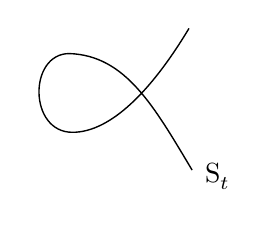
\begin{tikzpicture}[x=0.8cm,y=0.8cm,baseline=0pt]
\draw[line width=0.5pt]
 (1.05,1.05)
 .. controls (0.45,0.05) and (-0.20,-0.60) .. (-0.80,-0.60)
 .. controls (-1.50,-0.60) and (-1.50,0.65) .. (-0.85,0.65)
 .. controls (0.05,0.62) and (0.50,-0.20) .. (1.10,-1.20);
\node[anchor=west] at (1.15,-1.30) {\(\mathrm S_t\)};
\end{tikzpicture}
}
\&
{
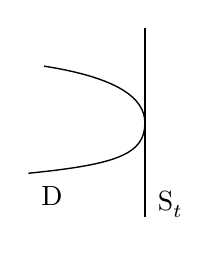
\begin{tikzpicture}[x=0.8cm,y=0.8cm,baseline=0pt]
\draw[line width=0.5pt] (0.60,-1.50)--(0.60,1.50);
\draw[line width=0.5pt]
 (-1.00,0.90)
 .. controls (0.15,0.72) and (0.60,0.40) .. (0.60,0)
 .. controls (0.60,-0.50) and (0.15,-0.66) .. (-1.25,-0.80);
\node[anchor=north west] at (-1.20,-0.85) {\(\mathrm D\)};
\node[anchor=west] at (0.65,-1.30) {\(\mathrm S_t\)};
\end{tikzpicture}
}
\&
{
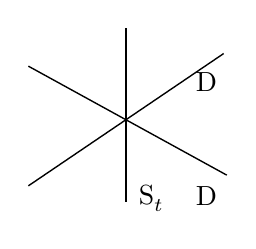
\begin{tikzpicture}[x=0.8cm,y=0.8cm,baseline=0pt]
\draw[line width=0.5pt] (0,-1.30)--(0,1.45);
\draw[line width=0.5pt] (-1.55,-1.05)--(1.55,1.05);
\draw[line width=0.5pt] (-1.55,0.85)--(1.60,-0.88);
\node[anchor=north east] at (1.60,0.90) {\(\mathrm D\)};
\node[anchor=north east] at (1.60,-0.90) {\(\mathrm D\)};
\node[anchor=west] at (0.05,-1.25) {\(\mathrm S_t\)};
\end{tikzpicture}
}
\\
{
\begin{array}{@{}ll@{}}
\text{\small\textit{a)}} & \text{\small curve with a double point}\\
 & \text{\small with distinct tangents;}
\end{array}
}
\&
{
\begin{array}{@{}ll@{}}
\text{\small\textit{b)}} & \text{\small tangency of \(\mathrm D\)}\\
 & \text{\small with \(\mathrm S_t\);}
\end{array}
}
\&
{
\begin{array}{@{}ll@{}}
\text{\small\textit{c)}} & \text{\small two branches of \(\mathrm D\)}\\
 & \text{\small intersect on \(\mathrm S_t\).}
\end{array}
}
\end{tikzcd}
\tag*{\textbf{(3.1.1.2)}}
\]

The cohomologies of \(\mathrm V\) and \(\widetilde{\mathrm V}\) are related by a canonical isomorphism:
\[
\mathrm H_c^*(\widetilde{\mathrm V},\pi^*\mathscr F)
\cong
\mathrm H_c^*(\mathrm V,\mathscr F)
\oplus
(\mathrm H^0(\mathrm V\cap\mathrm A,\mathscr F)(-1)
 \text{ placed in degree }2).
\tag*{\textbf{(3.1.1.3)}}
\]

For what follows, it would suffice to know the injectivity of:
\[
\pi^*:\mathrm H_c^*(\mathrm V,\mathscr F)
\hookrightarrow
\mathrm H_c^*(\widetilde{\mathrm V},\pi^*\mathscr F);
\tag*{\textbf{(3.1.1.4)}}
\]
the transpose under Poincaré duality of \(\pi^*:\mathrm H^*(\mathrm V,\mathscr F)\to\mathrm H^*(\widetilde{\mathrm V},\pi^*\mathscr F)\) is a retraction of (3.1.1.4).

To study the cohomology of \(\widetilde{\mathrm V}\), we shall use the Leray spectral sequence:
\[
\mathrm E_2^{pq}
=\mathrm H^p(\mathrm A^*,\mathrm R^qf_!\pi^*\mathscr F)
\Rightarrow
\mathrm H_c^{p+q}(\widetilde{\mathrm V},\pi^*\mathscr F).
\tag*{\textbf{(3.1.1.5)}}
\]

The sheaves \(\mathrm R^qf_!\pi^*\mathscr F=\mathrm R^qf_*(j_!\pi^*\mathscr F)\) are smooth, except at the exceptional values of \(f\).

Let \(t\) be an exceptional value of \(f\), \(\mathrm A^*_{(t)}\) the henselization of \(\mathrm A^*\) at \(t\) (a strictly henselian trait), and \(\bar{\eta}\) a geometric generic point of \(\mathrm A^*_{(t)}\). Let us apply the theory of vanishing cycles to the inverse image of \(\widetilde{\mathrm S}\), \(j_!\pi^*\mathscr F\), over \(\mathrm A^*_{(t)}\). The sheaves of vanishing cycles \(\Phi^q=\Phi^q(j_!\pi^*\mathscr F)\) are concentrated at the exceptional point \(x\) of \(\mathrm S_t\), and we obtain a long exact sequence:
\[
\ldots\xrightarrow{\partial}
(\mathrm R^qf_!\pi^*\mathscr F)_t
\to
(\mathrm R^qf_!\pi^*\mathscr F)_{\bar{\eta}}
\to\Phi_x^q\xrightarrow{\partial}\ldots
\tag*{\textbf{(3.1.1.6)}}
\]

\textbf{(3.1.2)} We propose to compute the \(\Phi_x^q\), or rather their associated graded object for a suitable filtration, under the following additional hypothesis.

(E) The local monodromy of \(\mathscr F\) around \(\mathrm D\) is unipotent.

Let \(d\in\mathrm D\), let \(\mathrm S_{(d)}\) be the strict localization of \(\mathrm S\) at \(d\), and let \(\mathrm V_{(d)}\) be the inverse image of \(\mathrm V\) in \(\mathrm S_{(d)}\). Hypothesis (E) ensures that the inverse image of \(\mathscr F\) on \(\mathrm V_{(d)}\) admits a finite filtration \(\mathrm F\) (by smooth subsheaves) such that the sheaves \(\operatorname{Gr}_{\mathrm F}^i(\mathscr F)\) are constant on \(\mathrm V_{(d)}\). We denote by \(\operatorname{Gr}_{\mathrm F}^i(\mathscr F)_d\) the stalk at \(d\) of the constant extension of \(\operatorname{Gr}_{\mathrm F}^i(\mathscr F)\) to \(\mathrm S_{(d)}\): it is \(\mathrm H^0(\mathrm V_{(d)},\operatorname{Gr}_{\mathrm F}^i(\mathscr F))\).

\Page{199}

We shall use the following notation: if \(\mathrm B\) is a two-element set, \(\varepsilon(\mathrm B)\) is a group equipped with two opposite isomorphisms with \(\mathbf Z\), indexed by \(\mathrm B\). For example, \(\bigwedge\limits^{2}\mathbf Z^{\mathrm B}\) or \(\mathbf Z^{\mathrm B}/(\mathbf Z\text{ diagonal})\).

Let us distinguish three cases, according to the nature of the exceptional point \(x\) of \(\mathrm S_t\) (3.1.1.2).

\textbf{(3.1.3)} \textit{Case} (a). — Since \(j_!\pi^*\mathscr F\) is smooth at \(x\), we have \(\Phi_x^*(j_!\pi^*\mathscr F)=\Phi_x^*(\overline{\mathbf Q}_\ell)\otimes\mathscr F_x\), and \(\Phi_x^*(\overline{\mathbf Q}_\ell)\) is given by Picard-Lefschetz theory (in relative dimension \(1\)): \(\Phi_x^q(\overline{\mathbf Q}_\ell)=0\) if \(q\ne1\), and if \(\mathrm B\) is the two-element set of branches of \(\widetilde{\mathrm S}_t\) at \(x\), we have \(\Phi_x^1(\overline{\mathbf Q}_\ell)=\overline{\mathbf Q}_\ell(-1)\otimes\varepsilon(\mathrm B)\). Altogether:
\[
\Phi_x^q(j_!\pi^*\mathscr F)=0
\qquad\text{for}\quad q\ne1
\quad\text{and}
\tag*{\textbf{(3.1.3.1)}}
\]
\[
\Phi_x^1(j_!\pi^*\mathscr F)
\cong\mathscr F_x(-1)\otimes\varepsilon(\mathrm B).
\tag*{\textbf{(3.1.3.2)}}
\]

The isomorphism (3.1.3.2) can be described as follows (we shall not use this description). If \(\mathrm W\) is the variety of vanishing cycles at \(x\), it arises from isomorphisms:
\[
\mathbf Z/\ell^n
\xrightarrow{\sim}
\mathrm H^1(\mathrm W,\mu_{\ell^n})
=\Phi_x^1(\mathbf Z/\ell^n(1));
\tag*{\textbf{(3.1.3.3)}}
\]
if \(u\) and \(v\) are local equations for the two branches of \(\mathrm S_t\) at \(x\), the canonical generator of \(\mathrm H^1(\mathrm W,\mu_{\ell^n})\) is defined by the Kummer covering \(\mathrm T^{\ell^n}=uv^{-1}\).

\textbf{(3.1.4)} \textit{Case} (b). — First suppose that \(\mathscr F\) is the constant sheaf \(\overline{\mathbf Q}_\ell\). Consider the short exact sequence:
\[
0\to j_!\overline{\mathbf Q}_\ell
\to\overline{\mathbf Q}_\ell
\to\overline{\mathbf Q}_{\ell\mathrm D}\to0.
\tag*{\textbf{(3.1.4.1)}}
\]

The groups of vanishing cycles \(\Phi_x^*\) vanish for the constant sheaf \(\overline{\mathbf Q}_\ell\), since \(f\) is smooth at \(x\). For \(\overline{\mathbf Q}_{\ell\mathrm D}\), they coincide with the analogous group computed on \(\mathrm D\), and the long exact sequence obtained from (3.1.4.1) by applying the cohomological functor \(\Phi_x^*\) gives isomorphisms:
\[
\Phi_x^q(j_!\overline{\mathbf Q}_\ell)
\cong\Phi_x^{q-1}(\mathrm D,\overline{\mathbf Q}_\ell).
\tag*{\textbf{(3.1.4.2)}}
\]

If \(\mathrm B\) is the set of the two points of the henselization \(\mathrm D_{(x)}\) above \(\bar{\eta}\), we therefore have:
\[
\Phi_x^q(j_!\overline{\mathbf Q}_\ell)=0
\qquad\text{for}\quad q\ne1
\quad\text{and}
\tag*{\textbf{(3.1.4.3)}}
\]
\[
\Phi_x^1(j_!\overline{\mathbf Q}_\ell)
=\overline{\mathbf Q}_\ell\otimes\varepsilon(\mathrm B).
\tag*{\textbf{(3.1.4.4)}}
\]

In the general case, let \(\mathrm F\) be a filtration as in (3.1.2). We find by dévissage that:
\[
\Phi_x^q(j_!\pi^*\mathscr F)=0
\qquad\text{for}\quad q\ne1
\tag*{\textbf{(3.1.4.5)}}
\]
and that \(\Phi_x^1(j_!\pi^*\mathscr F)\) admits a filtration \(\mathrm F\), for which:
\[
\operatorname{Gr}_{\mathrm F}^i\Phi_x^1(j_!\pi^*\mathscr F)
=\operatorname{Gr}_{\mathrm F}^i(\mathscr F)_x\otimes\varepsilon(\mathrm B).
\tag*{\textbf{(3.1.4.6)}}
\]

\Page{200}

\textbf{(3.1.5)} \textit{Case} (c). — Let \(\mathrm B\) be the two-element set of branches of \(\mathrm D\) through \(x\). Denoting by \(i\) the projection into \(\mathrm S\) or \(\widetilde{\mathrm S}\) from the normalization \(\mathrm D'\) of \(\mathrm D\), we have an exact sequence in a neighborhood of \(x\):
\[
0\to j_!\overline{\mathbf Q}_\ell
\to\overline{\mathbf Q}_\ell
\to i_*\overline{\mathbf Q}_\ell
\to\overline{\mathbf Q}_{\ell x}\otimes\varepsilon(\mathrm B)
\to0.
\tag*{\textbf{(3.1.5.1)}}
\]

Since \(f\) is smooth at \(x\), and \(f\circ i\) is smooth at the two points of \(\mathrm D'\) above \(x\), the sheaves \(\Phi_x^*\) vanish for \(\overline{\mathbf Q}_\ell\) and \(i_*\overline{\mathbf Q}_\ell\). We therefore obtain isomorphisms:
\[
\Phi_x^q(j_!\overline{\mathbf Q}_\ell)
=\Phi_x^{q-2}(x,\overline{\mathbf Q}_{\ell x}\otimes\varepsilon(\mathrm B)).
\tag*{\textbf{(3.1.5.2)}}
\]

The \(\Phi_x^q(x,\overline{\mathbf Q}_{\ell x}\otimes\varepsilon(\mathrm B))\) vanish for \(q\ne-1\), and \(\Phi_x^{-1}(x,\overline{\mathbf Q}_{\ell x}\otimes\varepsilon(\mathrm B))=\overline{\mathbf Q}_\ell\otimes\varepsilon(\mathrm B)\). This gives the value of the \(\Phi_x^q(j_!\overline{\mathbf Q}_\ell)\) and, by dévissage, that of \(\Phi_x^q(j_!\pi^*\mathscr F)\):
\[
\Phi_x^q(j_!\pi^*\mathscr F)=0
\qquad\text{for}\quad q\ne1,
\tag*{\textbf{(3.1.5.3)}}
\]
and, for \(\mathrm F\) as in (3.1.2):
\[
\operatorname{Gr}_{\mathrm F}^i\Phi_x^1(j_!\pi^*\mathscr F)
=\operatorname{Gr}_{\mathrm F}^i(\mathscr F)_x\otimes\varepsilon(\mathrm B).
\tag*{\textbf{(3.1.5.4)}}
\]

\section*{(3.2) — Dimension 1}

\textit{The conventions of \textup{(0.7)} are in force.}

\textit{Proposition} \textbf{(3.2.1)}. — \textit{Let \(\mathrm X_0\) be a smooth absolutely irreducible curve over \(\mathbf F_q\), and let \(\mathscr F_0\) be a smooth pointwise \(\iota\)-pure and \(\iota\)-real sheaf on \(\mathrm X_0\). Then the polynomials \(\iota\det(1-\mathrm F t,\mathrm H_c^i(\mathrm X,\mathscr F))\) have real coefficients.}

In Grothendieck’s formula, (1.4.7.1), the factors on the left-hand side are real polynomials by hypothesis, and the rational function on the right-hand side is real. Let \(\beta\) be the weight of \(\mathscr F_0\). By (1.4.4) and (2.2.10), the zeros of \(\iota\det(1-\mathrm F t,\mathrm H_c^2(\mathrm X,\mathscr F))\) (counted with multiplicity) are the poles of this rational function that have absolute value \(q^{-(\beta+2)/2}\). Their set is stable under complex conjugation, and the polynomial \(\iota\det(1-\mathrm F t,\mathrm H_c^2(\mathrm X,\mathscr F))\) is real. If \(\mathrm X_0\) is affine, \(\mathrm H_c^0\) vanishes. If \(\mathrm X_0\) is projective, it is the dual of \(\mathrm H_c^2(\mathrm X,\mathscr F^\vee(-1))\) (Poincaré duality), and since the polynomial \(\iota\det(1-\mathrm F t,\mathrm H^2(\mathrm X,\mathscr F^\vee(-1)))\) is real, we find in all cases that the polynomial \(\iota\det(1-\mathrm F t,\mathrm H_c^0(\mathrm X,\mathscr F))\) is real. The denominator on the right-hand side of (1.4.7.1) is therefore real, and the numerator \(\iota\det(1-\mathrm F t,\mathrm H_c^1(\mathrm X,\mathscr F))\) must be real as well.

\textit{Remark} \textbf{(3.2.2)}. — The arguments of (0.5) show that (3.2.1) holds without the hypothesis of absolute irreducibility.

\textit{Theorem} \textbf{(3.2.3)}. — \textit{Let \(\mathrm X_0\) be a smooth projective curve over \(\mathbf F_q\), \(j:\mathrm U_0\hookrightarrow\mathrm X_0\) a dense open subset of \(\mathrm X_0\), and \(\mathscr F_0\) a smooth pointwise \(\iota\)-pure sheaf of weight \(\beta\) on \(\mathrm U_0\). Then the eigenvalues \(\alpha\) of \(\mathrm F\) on \(\mathrm H^i(\mathrm X,j_*\mathscr F)\) satisfy \(w_q(\alpha)=\beta+i\).}

% ---- 201-208 ----
\Page{201}

For a description of the main lines of the proof, I refer to the introduction. For \(i=1\), the group \(\mathrm{H}^1(\mathrm{X},j_*\mathscr{F})\) is also the image of \(\mathrm{H}_c^1(\mathrm{U},\mathscr{F})\) in \(\mathrm{H}^1(\mathrm{U},\mathscr{F})\) (cf. the “parabolic” cohomology groups encountered in the study of modular forms).

We shall begin by proving by induction on \(k\) the following proposition, which, for \(k=0\), follows from (1.8.2).

\textit{Lemma} \textbf{(3.2.4)} \((k)\). — \textit{Let \(\mathrm{U}_0\) be a smooth curve over \(\mathbf{F}_q\) and \(\mathscr{F}_0\) a smooth pointwise \(\iota\)-pure sheaf of weight \(0\) on \(\mathrm{U}_0\). Then the eigenvalues \(\alpha\) of \(\mathrm{F}\) on \(\mathrm{H}_c^1(\mathrm{U},\mathscr{F})\) satisfy \(w_q(\alpha)\leq 1+2^{-k}\).}

\textbf{(3.2.5)} \((k)\) If \(\mathrm{U}_0\) is a dense open subset of a curve \(\mathrm{X}_0\): \(j:\mathrm{U}_0\hookrightarrow\mathrm{X}_0\), and \(\mathscr{G}_0\) is a sheaf on \(\mathrm{X}_0\), the long exact cohomology sequence defined by the short exact sequence \(0\to j_!j^*\mathscr{G}_0\to\mathscr{G}_0\to\mathscr{G}_0/j_!j^*\mathscr{G}_0\to0\) gives a surjection:
\[
\mathrm{H}_c^1(\mathrm{U},j^*\mathscr{G})
=\mathrm{H}_c^1(\mathrm{X},j_!j^*\mathscr{G})
\twoheadrightarrow\mathrm{H}_c^1(\mathrm{X},\mathscr{G}).
\]
If \(\mathrm{U}_0\) is smooth, and \(j^*\mathscr{G}_0\) is smooth and pointwise \(\iota\)-pure of weight \(\beta\), it therefore follows from (3.2.4) \((k)\) and a twisting argument (1.2.7) that the eigenvalues of \(\mathrm{F}\) on \(\mathrm{H}_c^1(\mathrm{X},\mathscr{G})\) satisfy \(w_q(\alpha)\leq\beta+1+2^{-k}\).

\textbf{(3.2.6)} Let \(k\geq0\). Assume (3.2.4) \((k)\) (and its corollary (3.2.5) \((k)\)) and let us prove (3.2.4) \((k+1)\). We shall first do so under hypotheses (A) to (C) below. Let \(\mathrm{X}_0\) be the smooth projective curve of which \(\mathrm{U}_0\) is a dense open subset.

(A) The sheaf \(\mathscr{F}\) on \(\mathrm{U}\) is tamely ramified, with unipotent local monodromy, at the points of \(\mathrm{X}-\mathrm{U}\).

Let \(\mathrm{S}_0=\mathrm{X}_0\times\mathrm{X}_0\), \(\mathrm{V}_0=\mathrm{U}_0\times\mathrm{U}_0\), and let \(\mathrm{D}_0\) be the divisor with normal crossings on \(\mathrm{S}_0\) whose complement is \(\mathrm{V}_0\); let us embed \(\mathrm{S}_0\) in a projective space \(\mathbf{P}_0\) and sweep out \(\mathrm{S}_0\) by a pencil of hyperplanes with axis \(\mathrm{A}_0\subset\mathbf{P}_0\). We assume that the embedding and the pencil can be chosen so that

(B) \(\mathrm{S}\), \(\mathrm{D}\), and the pencil of hyperplane sections with axis \(\mathrm{A}\) satisfy the general-position conditions (A) to (D) of (3.1.1).

Finally, we shall make the following hypothesis for convenience:

(C) The exceptional points (3.1.1) are defined over \(\mathbf{F}_q\).

The arrows of diagram (3.1.1.1) arise by extension of scalars from morphisms of \(\mathbf{F}_q\)-schemes, which we shall denote by the same letters \(f\), \(\pi\), \(j\). We shall denote by \(\mathrm{T}_0\) the finite set of exceptional values of \(f\), by \(\mathrm{W}_0\) the complement of \(\mathrm{T}_0\) in \(\mathrm{A}_0^*\), and by \(w\) the inclusion of \(\mathrm{W}_0\) in \(\mathrm{A}_0^*\).

Let \(\mathscr{G}_0=\mathscr{F}_0\boxtimes\mathscr{F}_0=\operatorname{pr}_1^*\mathscr{F}_0\otimes\operatorname{pr}_2^*\mathscr{F}_0\) be the external tensor product of \(\mathscr{F}_0\) with itself. We shall apply the theory (3.1) to the calculation of the cohomology of \(\mathscr{G}\). By hypothesis, the hypotheses (A) to (E) of (3.1) are satisfied by \((\mathrm{S},\mathrm{D},\mathscr{G})\) and the pencil with axis \(\mathrm{A}\).

\Page{202}

\textit{Lemma} \textbf{(3.2.7)}. — \textit{The smooth sheaf \(w^*\mathrm{R}^1f_!\pi^*\mathscr{G}_0\) on \(\mathrm{W}_0\) is a direct factor of an \(\iota\)-real sheaf.}

\textit{Proof.} — Since the sheaf \(\mathscr{G}\) is smooth and pointwise \(\iota\)-pure of weight \(0\), the sheaf \(\mathscr{H}_0=\mathscr{G}_0\oplus\mathscr{G}_0^\vee\) is pointwise \(\iota\)-pure and \(\iota\)-real, and it suffices to verify that the sheaf \(\mathrm{R}^1f_!\pi^*\mathscr{H}_0\) on \(\mathrm{W}_0\) is \(\iota\)-real. This is a consequence of (3.2.1): if \(x\in|\mathrm{W}_0|\), if \(\mathrm{Y}_1\) is the fiber of  \(f:\widetilde{\mathrm{V}}_0\to\mathrm{A}_0^*\) at \(x\) (a curve over \(k(x)\)), and if \(\mathrm{Y}\) is obtained from \(\mathrm{Y}_1\) by the extension of scalars from \(k(x)\) to \(\mathbf{F}\) defined by a geometric point \(\bar{x}\) localized at \(x\), we have:
\[
(\mathrm{R}^1f_!\pi^*\mathscr{H}_0)_{\bar{x}}
=\mathrm{H}_c^1(\mathrm{Y},\pi^*\mathscr{H})
\tag*{\textbf{(3.2.7.1)}}
\]
and we apply (3.2.2) for \(i=1\) and to the restriction of \(\pi^*\mathscr{H}\) to \(\mathrm{Y}_1\).

We shall prove Lemmas (3.2.8) and (3.2.9) below together.

\textit{Lemma} \textbf{(3.2.8)}. — \textit{The sheaf \(\mathrm{R}^1f_!\pi^*\mathscr{G}\) has no section supported in \(\mathrm{T}\).}

This lemma allows us to identify \(\mathrm{R}^1f_!\pi^*\mathscr{G}_0\) with a subsheaf of \(w_*w^*\mathrm{R}^1f_!\pi^*\mathscr{G}_0\). By (3.2.7) and (1.5.1), the sheaf \(w^*\mathrm{R}^1f_!\pi^*\mathscr{G}_0\) admits a finite filtration \(\mathrm{G}^\bullet\) with smooth pointwise \(\iota\)-pure successive quotients. We extend it to a finite filtration of \(\mathrm{R}^1f_!\pi^*\mathscr{G}_0\) by the formula:
\[
\mathrm{G}^i\mathrm{R}^1f_!\pi^*\mathscr{G}_0
=w_*\mathrm{G}^iw^*\mathrm{R}^1f_!\pi^*\mathscr{G}_0
\cap\mathrm{R}^1f_!\pi^*\mathscr{G}_0
\]
(intersection in \(w_*w^*\mathrm{R}^1f_!\pi^*\mathscr{G}_0\)).

\textit{Lemma} \textbf{(3.2.9)}. — \textit{If \(\operatorname{Gr}_{\mathrm{G}}^i\mathrm{R}^1f_!\pi^*\mathscr{G}_0\) does not become constant on \(\mathrm{A}^*\), its restriction to \(\mathrm{W}_0\) is pointwise \(\iota\)-pure of integral weight.}

Let \(\bar{x}\in\mathrm{X}-\mathrm{U}\), let \(x\) be its image in \(\mathrm{X}_0-\mathrm{U}_0\), let \(\eta\) be the generic point of \(\mathrm{X}_{0(x)}\), and let \(\bar{\eta}\) be a geometric point localized at the generic point of \(\mathrm{X}_{(\bar{x})}\). By (1.8.4), the representation \(\mathscr{F}_{0\bar{\eta}}\) of the Weil group \(\mathrm{W}(\bar{\eta}/\eta)\) admits a filtration with successive quotients that are \(\iota\)-pure of integral weights. Hypothesis (A) further implies that inertia acts trivially on these quotients. For \(x\in\mathrm{U}_0\), the same conclusion holds by hypothesis for the trivial filtration, with a single step.

Let \(x\in\mathrm{S}_0-\mathrm{V}_0\), let \(\bar{x}\) be a geometric point localized at \(x\), let \(\mathrm{S}_{0(x)}\) be the henselization of \(\mathrm{S}_0\) at \(x\), and let \(\mathrm{V}_{0(x)}\) be the inverse image of \(\mathrm{V}_0\) in \(\mathrm{S}_{0(x)}\). Taking the tensor product, we find that \(\mathscr{G}_0\) admits on \(\mathrm{V}_{0(x)}\) a finite filtration \(\mathrm{F}\), such that the \(\operatorname{Gr}_{\mathrm{F}}^i\mathscr{G}_0\) are constant on \(\mathrm{V}_{(x)}\) and the \(\operatorname{Gr}_{\mathrm{F}}^i(\mathscr{G}_0)_{\bar{x}}\) (notation (3.1.2)) are \(\iota\)-pure of integral weights. For \(x\in\mathrm{V}_0\), \(\mathscr{G}_{\bar{x}}\) itself is \(\iota\)-pure of integral weight (namely, \(0\)).

Let \(\bar{t}\in\mathrm{T}\), let \(x\in\widetilde{\mathrm{S}}\) be the exceptional point above it (3.1.1), let \(t\) and \(x\) be their images in \(\mathrm{T}_0\) and \(\mathrm{S}_0\), let \(\bar{\eta}\) be a geometric point localized at the generic point of \(\mathrm{A}_{(t)}^*\), and let \(\eta\) be the generic point of \(\mathrm{A}_{0(t)}^*\). Since the sheaves of vanishing cycles, computed in n\textsuperscript{o} (3.1), are concentrated at \(x\) and vanish for \(i\neq1\), we obtain a five-term exact sequence:
\[
0\to(\mathrm{R}^1f_!\pi^*\mathscr{G}_0)_{\bar{t}}
\to(\mathrm{R}^1f_!\pi^*\mathscr{G}_0)_{\bar{\eta}}
\to\Phi_{\bar{x}}^1
\to(\mathrm{R}^2f_!\pi^*\mathscr{G}_0)_{\bar{t}}
\to(\mathrm{R}^2f_!\pi^*\mathscr{G}_0)_{\bar{\eta}}\to0.
\tag*{\textbf{(3.2.9.1)}}
\]

\Page{203}

Injectivity on the left ensures that \(\mathrm{R}^1f_!\bar{u}_*\mathscr{G}\) has no section supported at \(t\). This proves (3.2.8). We also obtain short exact sequences:
\[
0\to\operatorname{Gr}_{\mathrm{G}}^i
(\mathrm{R}^1f_!\pi^*\mathscr{G}_0)_{\bar{t}}
\to\operatorname{Gr}_{\mathrm{G}}^i
(\mathrm{R}^1f_!\pi^*\mathscr{G}_0)_{\bar{\eta}}
\to\mathrm{A}_t^i\to0,
\]
where \(\mathrm{A}_t^i\) is a subquotient of \(\Phi_{\bar{x}}^1\). The calculation (3.1) ensures that \(\Phi_{\bar{x}}^1\), and hence \(\mathrm{A}_t^i\), admits a filtration with successive quotients that are \(\iota\)-pure of integral weight. By (1.8.4), if \(\mathrm{A}_t^i\neq0\), the \(\iota\)-pure sheaf \(w^*\operatorname{Gr}_{\mathrm{G}}^i(\mathrm{R}^1f_!\pi^*\mathscr{G}_0)\) is therefore of integral weight.

To conclude, note that if, for fixed \(i\), all the \(\mathrm{A}_t^i\) vanish, the sheaf \(\operatorname{Gr}_{\mathrm{G}}^i\mathrm{R}^1f_!\pi^*\mathscr{G}_0\) is smooth, hence constant on \(\mathrm{A}^*\), since the projective line \(\mathrm{A}^*\) is simply connected.

\textit{Lemma} \textbf{(3.2.10)}. — \textit{The constituents of \(w^*\mathrm{R}^1f_!\pi^*\mathscr{G}_0\) are pointwise \(\iota\)-pure of weights \(<2\).}

We know that the constituents are pointwise \(\iota\)-pure. It suffices to test the weights at one point. The lemma follows from (2.2.10) (cf. (3.2.7.1)).

\textit{Lemma} \textbf{(3.2.11)}. — \textit{The eigenvalues \(\alpha\) of \(\mathrm{F}\) on \(\mathrm{E}_2^{11}=\mathrm{H}^1(\mathrm{A}^*,\mathrm{R}^1f_!\pi^*\mathscr{G})\) satisfy \(w_q(\alpha)\leq2+2^{-k}\).}

It suffices to verify this for the eigenvalues of \(\mathrm{F}\) on each \(\mathrm{H}^1(\mathrm{A}^*,\operatorname{Gr}_{\mathrm{G}}^i\mathrm{R}^1f_!\pi^*\mathscr{G})\). If \(\operatorname{Gr}_{\mathrm{G}}^i\mathrm{R}^1f_!\pi^*\mathscr{G}\) is constant, this \(\mathrm{H}^1\) vanishes, since \(\mathrm{A}^*\) is a projective line. Otherwise, \(w^*\operatorname{Gr}_{\mathrm{G}}^i\mathrm{R}^1f_!\pi^*\mathscr{G}\) has integral weight \(<2\) ((3.2.9) and (3.2.10)), hence weight \(\leq1\), and we apply (3.2.5) \((k)\).

\textit{Lemma} \textbf{(3.2.12)}. — \textit{The eigenvalues \(\alpha\) of \(\mathrm{F}\) on \(\mathrm{E}_2^{02}=\mathrm{H}^0(\mathrm{A}^*,\mathrm{R}^2f_!\pi^*\mathscr{G})\) and on \(\mathrm{E}_2^{20}=\mathrm{H}^2(\mathrm{A}^*,\mathrm{R}^0f_!\pi^*\mathscr{G})\) satisfy \(w_q(\alpha)\leq2\).}

Formula (3.2.7.1), and two applications of (1.4.4), show that, for \(x\in|\mathrm{A}_0^*|\), the eigenvalues \(\alpha\) of \(\mathrm{F}_x\) on \(\mathrm{R}^if_!\pi^*\mathscr{G}_0\) \((i=0,2)\) satisfy \(w_{\mathrm{N}(x)}(\alpha)\leq i\), and then yield the assertion.

\textbf{(3.2.13)} \textit{Proof of} (3.2.4) \((k+1)\) \textit{under the hypotheses} (3.2.6).

It follows from (3.2.11), (3.2.12), and the spectral sequence (3.1.1.5) that the eigenvalues \(\alpha\) of \(\mathrm{F}\) on \(\mathrm{H}_c^2(\widetilde{\mathrm{V}},\pi^*\mathscr{G})\) satisfy \(w_q(\alpha)\leq2+2^{-k}\).

The same estimate holds \textit{a fortiori} for the eigenvalues of \(\mathrm{F}\) on:
\[
\mathrm{H}_c^1(\mathrm{U},\mathscr{F})\otimes
\mathrm{H}_c^1(\mathrm{U},\mathscr{F})
\subset\mathrm{H}_c^2(\mathrm{V},\mathscr{G})
\subset\mathrm{H}_c^2(\widetilde{\mathrm{V}},\pi^*\mathscr{G})
\]
(Künneth and (3.1.1.4)). In particular, if \(\alpha\) is an eigenvalue of \(\mathrm{F}\) on \(\mathrm{H}_c^1(\mathrm{U},\mathscr{F})\), we have \(w_q(\alpha^2)\leq2+2^{-k}\), hence \(w_q(\alpha)\leq1+2^{-(k+1)}\).

\textbf{(3.2.14)} \textit{End of the proof of} (3.2.4) \((k+1)\). — The validity of assertion (3.2.4) \((k+1)\) is invariant under a preliminary extension of the finite base field \(\mathbf{F}_q\) (cf. the proof of (2.2.10)). Since, over \(\mathbf{F}\), there exist embeddings and pencils satis-\Page{204}fying (B), such embeddings and pencils also exist over a finite extension of \(\mathbf{F}_q\). Over a larger finite extension, (C) will be satisfied. This proves (3.2.4) \((k+1)\) under hypothesis (A) alone.

The monodromy theorem ensures that there exists a finite surjective covering \(g:\mathrm{U}'_0\to\mathrm{U}_0\), with \(\mathrm{U}'_0\) smooth, such that \(g^*\mathscr{F}_0\) on \(\mathrm{U}'_0\) satisfies (A); we conclude by noting that the morphism \(g^*\) injects \(\mathrm{H}_c^*(\mathrm{U},\mathscr{F})\) into \(\mathrm{H}_c^*(\mathrm{U}',g^*\mathscr{F})\).

\textbf{(3.2.15)} \textit{Proof of} (3.2.3). — The assertion is trivial for \(i=0\) or \(2\) (1.4). For \(i=1\), the validity of (3.2.5) \((k)\) for every \(k_1\) ensures that \(w_q(\alpha)\leq\beta+1\). Let us apply this result to the sheaf \(\mathscr{F}_0^\vee(1)\). Since \(\mathrm{H}^1(\mathrm{X},j_*\mathscr{F})\) and \(\mathrm{H}^1(\mathrm{X},j_*\mathscr{F}^\vee(1))\) are in duality (SGA \(4\frac{1}{2}\) [duality] (1.3) and (2.1)), we find that \(w_q(\alpha^{-1})\leq(-\beta-2)+1\), i.e. that \(w_q(\alpha)\geq\beta+1\). The theorem follows.

\section*{(3.3) — The general case}

\textit{Theorem} \textbf{(3.3.1)}. — \textit{Let \(f:\mathrm{X}\to\mathrm{Y}\) be a morphism of schemes of finite type over \(\mathbf{Z}\), and \(\mathscr{F}\) a sheaf on \(\mathrm{X}\). If \(\mathscr{F}\) is mixed of weights \(\leq n\), then, for each \(i\), \(\mathrm{R}^if_!\mathscr{F}\) is mixed of weights \(\leq n+i\).}

The proof uses the following dévissages:

a) \textit{Dévissages in \(\mathscr{F}\)}: Let \(0\to\mathscr{F}'\to\mathscr{F}\to\mathscr{F}''\to0\) be an exact sequence. If the \(\mathrm{R}^if_!\mathscr{F}'\) and \(\mathrm{R}^if_!\mathscr{F}''\) are mixed of weights \(\leq n+i\), then the \(\mathrm{R}^if_!\mathscr{F}\) are as well. If the \(\mathrm{R}^if_!\mathscr{F}\) and \(\mathrm{R}^if_!\mathscr{F}''\) are mixed of weights \(\leq n+i\), then the \(\mathrm{R}^if_!\mathscr{F}'\) are as well (apply the long exact cohomology sequence). If the sequence splits and \(\mathrm{R}^if_!\mathscr{F}\) is mixed of weights \(\leq n+i\), then \(\mathrm{R}^if_!\mathscr{F}'\) is as well.

b) \textit{Dévissage in \(\mathrm{X}\)}: Let \(j:\mathrm{U}\hookrightarrow\mathrm{X}\) be an open subset of \(\mathrm{X}\), with complement \(i:\mathrm{S}\to\mathrm{X}\). If the \(\mathrm{R}^i(fj)_!j^*\mathscr{F}\) and the \(\mathrm{R}^i(fi)_!i^*\mathscr{F}\) are mixed of weights \(\leq n+i\), the \(\mathrm{R}^if_!\mathscr{F}\) are as well (apply (a) to the short exact sequence \(0\to j_!j^*\mathscr{F}\to\mathscr{F}\to i_*i^*\mathscr{F}\to0\)).

c) \textit{Dévissage in \(\mathrm{Y}\)}: Let \(j:\mathrm{V}\hookrightarrow\mathrm{Y}\) be an open subset of \(\mathrm{Y}\), with complement \(i:\mathrm{T}\to\mathrm{Y}\). If the conclusion of (3.3.1) becomes true after the base changes by \(i\) and \(j\), it is true to begin with (apply the base change theorem).

d) \textit{Transitivity}: If \(f=gh\), and the \(\mathrm{R}^ig_!\mathrm{R}^jh_!\mathscr{F}\) are mixed of weights \(\leq n+i+j\), then the \(\mathrm{R}^kf_!\mathscr{F}\) are mixed of weights \(\leq n+k\) (apply the Leray spectral sequence \(\mathrm{R}^pg_!\mathrm{R}^qh_!\Rightarrow\mathrm{R}^{p+q}f_!\)).

e) If \(\mathrm{Y}'\xrightarrow{g}\mathrm{Y}\) is a universal homeomorphism, it suffices to verify (3.3.1) after base change by \(g\) (étale cohomology does not “see” such a base change). Examples: \(\mathrm{Y}'=\mathrm{Y}_{\mathrm{red}}\), or \(\mathrm{Y}'=\) the normalization of \(\mathrm{Y}\), assumed normal and integral, in an inseparable extension of its function field.

f) If \(f\) has relative dimension \(0\), and \(\mathscr{F}\) is pointwise pure, then \(f_!\mathscr{F}=\mathrm{R}^0f_!\mathscr{F}\) is pointwise pure of the same weight, and the \(\mathrm{R}^if_!\mathscr{F}\) vanish for \(i\neq0\). For such an \(f\), we conclude by (a).

\Page{205}

The dévissages (b), (c), (d) reduce us to assuming that \(f\) has relative dimension \(1\), and then (a), (b) reduce us to assuming that \(\mathscr{F}\) is smooth and pointwise pure of weight \(n\).

Note that if \(\mathrm{C}\) is a curve over a field \(\mathrm{K}\), and \(\mathscr{F}\) is a smooth sheaf on \(\mathrm{C}\), the following assertions hold for \(\mathrm{K}\) perfect, hence in the general case after a finite purely inseparable extension of \(\mathrm{K}\): \((\alpha)\) There exists a finite subset of \(\mathrm{C}_{\mathrm{red}}\) whose complement \(\mathrm{C}'\) is smooth over \(\mathrm{K}\). \((\beta)\) There exists a finite surjective covering \(u:\mathrm{D}\to\mathrm{C}'\), where \(\mathrm{D}\) is the complement, in a smooth projective curve \(\overline{\mathrm{D}}\), of a divisor \(\mathrm{E}\) étale over \(\mathrm{K}\), such that \(u^*\mathscr{F}\) is tamely ramified along \(\mathrm{E}\); \(\mathscr{F}\) is a direct factor of \(u_*u^*\mathscr{F}=\mathrm{R}u_*u^*\mathscr{F}\). We shall apply this to the fiber of \(f\) at a generic point \(\eta\) of \(\mathrm{Y}\). The usual limit arguments show that \(\mathrm{C}'\), \(\mathrm{D}\)\dots{} exist, with the same properties, over a neighborhood of \(\eta\) in \(\mathrm{Y}_{\mathrm{red}}\). By (c), (e), we reduce to assuming that this neighborhood is all of \(\mathrm{Y}_{\mathrm{red}}\) and that \(\mathrm{Y}_{\mathrm{red}}\) is smooth, and then by (b), (f), (a), to assuming that \(\mathrm{X}\) is the complement, in \(\overline{\mathrm{X}}\), projective and smooth of pure relative dimension \(1\) over \(\mathrm{Y}\), of a divisor \(\mathrm{D}\) finite étale over \(\mathrm{Y}\), and that \(\mathscr{F}\) is tamely ramified along \(\mathrm{D}\).
\[
\begin{tikzcd}[ampersand replacement=\&,column sep=1.2em,row sep=1.5em]
\mathrm{X} \arrow[rr,hook,"j"] \arrow[dr,"f"']
\& \&
\overline{\mathrm{X}} \arrow[dl,"\bar f"]
\& \&
\mathrm{D} \arrow[ll,hook',"i"']
\\
\& \mathrm{Y} \& \& \&
\end{tikzcd}
\]
We have \(\mathrm{R}f_!\mathscr{F}=\mathrm{R}\bar{f}_*(j_!\mathscr{F})\). Consider the exact sequence:
\[
0\to j_!\mathscr{F}\to j_*\mathscr{F}
\to i_!i^*j_*\mathscr{F}\to0
\]
and the filtration induced by the local monodromy filtration \(\mathrm{M}\) on \(i_!i^*j_*\mathscr{F}\) ((1.8.6) to (1.8.8)). Formation of these sheaves and of \(\mathrm{M}\) is compatible with passage to the fibers. Theorem (3.2.3), applied to all isomorphisms \(\iota\), therefore ensures that \(\mathrm{R}^i\bar{f}_*j_*\mathscr{F}\) is pointwise pure of weight \(n+i\), and Theorem (1.8.4) (also for every \(\iota\)) ensures that \(\operatorname{Gr}_{\mathrm{M}}^k(i^*j_*\mathscr{F})\), zero for \(k>0\), is pure of weight \(n+k\) on \(\mathrm{D}\) (1.8.8). The morphism \(\bar{f}i\) is finite, and it remains only to apply (f), (a).

\textbf{(3.3.2)} To \textit{obtain lower bounds for} the weights, we can use the results of SGA 7 XXI 5 on the \(p\)-adic valuations of Frobenius eigenvalues. Let us say that a sheaf is \textit{integral} if the Frobenius eigenvalues are algebraic integers. The weights of an integral mixed sheaf are necessarily nonnegative: if an algebraic integer \(\alpha\) is pure of weight \(n\), relative to \(q\), and of degree \(d\), its norm is an ordinary integer whose absolute value is the product \(q^{nd/2}\) of the absolute values of its complex conjugates, so that \(n\geq0\).

\textit{Corollary} \textbf{(3.3.3)}. — \textit{Let \(f:\mathrm{X}\to\mathrm{Y}\) be a morphism of schemes of finite type over \(\mathbf{Z}\) and \(\mathscr{F}\) an integral sheaf on \(\mathrm{X}\). If \(\mathscr{F}\) is mixed of weights \(\leq n\), then, for each \(i\), \(\mathrm{R}^if_!\mathscr{F}\) is mixed of weights between \(0\) and \(n+i\). If \(i\) exceeds the maximum dimension \(d\) of the fibers, the weights lie between \(2(i-d)\) and \(n+i\).}

By SGA 7 XXI (5.2.2), applied to the fibers of \(f\), the sheaves \(\mathrm{R}^if_!\mathscr{F}\) and \(\mathrm{R}^if_!\mathscr{F}(i-d)\) are indeed integral.

\Page{206}

When \(\mathrm{X}\) and \(\mathrm{Y}\) have characteristic \(p>0\), we can replace étale sheaves by Weil sheaves. The most important case is that in which \(\mathrm{Y}=\operatorname{Spec}(\mathbf{F}_q)\). In this case, (3.3.1) and (3.3.3) mean the following — with the notation (0.7):

\textit{Corollary} \textbf{(3.3.4)}. — \textit{Let \(\mathrm{X}_0\) be a scheme of finite type over \(\mathbf{F}_q\) and \(\mathscr{F}_0\) a mixed sheaf of weights \(\leq n\) on \(\mathrm{X}_0\). Then \(\mathrm{H}_c^i(\mathrm{X},\mathscr{F})\) is mixed of weights \(\leq n+i\): for each \(i\) and each eigenvalue \(\alpha\) of \(\mathrm{F}\) on \(\mathrm{H}_c^i(\mathrm{X},\mathscr{F})\), \(\alpha\) is algebraic and there exists an integer \(w\leq n+i\) such that all the complex conjugates of \(\alpha\) have absolute value \(q^{w/2}\). If \(\mathscr{F}_0\) is integral, we have \(w\geq0\). If, in addition, \(i\) exceeds the dimension \(d\) of \(\mathrm{X}\), we have \(w\geq2(i-d)\).}

\textit{Corollary} \textbf{(3.3.5)}. — \textit{Let \(\mathrm{X}_0\) be smooth of finite type over \(\mathbf{F}_q\) and \(\mathscr{F}_0\) a smooth mixed sheaf of weights \(\geq n\) on \(\mathrm{X}_0\). Then \(\mathrm{H}^i(\mathrm{X},\mathscr{F})\) is mixed of weights \(\geq n+i\).}

We reduce to assuming that \(\mathrm{X}_0\) is of pure dimension \(\mathrm{N}\). Let \(\mathscr{F}_0^\vee\) be the dual sheaf of \(\mathscr{F}_0\). It is mixed of weights \(\leq-n\). By (3.3.3), the group \(\mathrm{H}_c^{2\mathrm{N}-i}(\mathrm{X},\mathscr{F}^\vee)(\mathrm{N})\) is mixed of weights \(\leq-n+(2\mathrm{N}-i)-2\mathrm{N}=-n-i\). Poincaré duality identifies \(\mathrm{H}^i(\mathrm{X},\mathscr{F})\) with its dual, mixed of weights \(\geq n+i\).

Combining the opposite inequalities of (3.3.4) and (3.3.5), we obtain the

\textit{Corollary} \textbf{(3.3.6)}. — \textit{Let \(\mathrm{X}_0\) be smooth of finite type over \(\mathbf{F}_q\) and \(\mathscr{F}_0\) a smooth pure sheaf of weight \(n\) on \(\mathrm{X}_0\). Then the image of \(\mathrm{H}_c^i(\mathrm{X},\mathscr{F})\) in \(\mathrm{H}^i(\mathrm{X},\mathscr{F})\) is pure of weight \(n+i\).}

In SGA \(4\frac{1}{2}\) [Trigonometric sums] I explain how these results make it possible to give upper bounds for certain trigonometric sums.

\textbf{(3.3.7)} Suppose \(\alpha\) is an algebraic number, pure of a weight \(n\), relative to \(q\), and let us normalize the \(p\)-adic valuations of \(\mathbf{Q}(\alpha)\) by requiring that \(v(q)=1\). To \(\alpha\), and to each valuation \(v\), let us attach the pair of rational numbers \((v(\alpha),v(q^n\alpha^{-1}))\), where \(q^n\alpha^{-1}=\bar{\alpha}\). If \(\alpha\) is integral, these numbers are \(\geq0\). Their sum is \(n\). For the constant sheaf \(\overline{\mathbf{Q}}_\ell\), (3.3.4) and the duality method (3.3.5) allow us to locate as follows the pairs \((r,s)\) attached to the Frobenius eigenvalues on an \(\mathrm{H}^i\).

\textit{Corollary} \textbf{(3.3.8)}. — \textit{Suppose \(\mathrm{X}\) has dimension \(\leq d\). In cohomology with compact support (or in ordinary cohomology for \(\mathrm{X}\) proper), \((r,s)\) lies in a lower triangle of the diagram below. In ordinary cohomology, and for \(\mathrm{X}\) smooth, \((r,s)\) lies in an upper triangle of the same diagram.}
\[
\begin{tikzcd}[
  ampersand replacement=\&,
  baseline=(current bounding box.south),
  row sep=0pt,
  column sep=0pt,
  cells={nodes={inner sep=0pt,outer sep=0pt,minimum size=0pt,text height=0pt,text depth=0pt}},
  arrows={shorten <=0pt,shorten >=0pt}
]
{} \&[1.8cm] {} \&[1.6cm] {}
\\[0.55cm]
{} \arrow[r,no head] \arrow[dr,no head]
\& {} \arrow[d,no head]
\& {}
\\[1.8cm]
{} \arrow[uu,"\textstyle s"{pos=.9,left}]
   \arrow[rr,"\textstyle r"{pos=.9,below}]
   \arrow[r,phantom,"\textstyle i"{pos=1,below}]
   \arrow[r,phantom,"\textstyle\text{if }i\leq d"{pos=1,below,yshift=-.55cm}]
   \arrow[ur,phantom,"\textstyle\mathrm{H}_c^i"{description,pos=.18}]
   \arrow[ur,phantom,"{\begin{gathered}\textstyle\mathrm{H}^i,\\[-.3ex]\textstyle\mathrm{X}\ \text{smooth}\end{gathered}}"{description,pos=.6,xshift=.25cm}]
\& {}
\& {}
\end{tikzcd}
\qquad
\begin{tikzcd}[
  ampersand replacement=\&,
  baseline=(current bounding box.south),
  row sep=0pt,
  column sep=0pt,
  cells={nodes={inner sep=0pt,outer sep=0pt,minimum size=0pt,text height=0pt,text depth=0pt}},
  arrows={shorten <=0pt,shorten >=0pt}
]
{} \&[.6cm] {} \&[1.8cm] {} \&[.6cm] {} \&[1.6cm] {}
\\[.6cm]
{} \arrow[r,no head]
\& {} \arrow[r,no head]
      \arrow[dr,no head,shorten <=-4mm,shorten >=-18mm]
\& {} \arrow[d,no head]
\& {}
\& {}
\\[1.8cm]
{}
\& {} \arrow[u,no head] \arrow[r,no head]
      \arrow[ur,phantom,"\textstyle\mathrm{H}_c^i"{description,pos=.18}]
      \arrow[ur,phantom,"{\begin{gathered}\textstyle\mathrm{H}^i,\\[-.3ex]\textstyle\mathrm{X}\ \text{smooth}\end{gathered}}"{description,pos=.65,xshift=.15cm}]
\& {} \arrow[d,no head]
\& {}
\& {}
\\[.6cm]
{} \arrow[uuu,"\textstyle s"{pos=.9,left}]
   \arrow[rrrr,"\textstyle r"{pos=.9,below}]
   \arrow[rr,phantom,"\textstyle d"{pos=1,below}]
   \arrow[rrr,phantom,"\textstyle i"{pos=1,below}]
   \arrow[rrr,phantom,"\textstyle\text{if }i\geq d"{pos=1,below,yshift=-.7cm}]
\& {}
\& {}
\& {}
\& {}
\end{tikzcd}
\]

\Page{207}

The verification is easy. One can show that, in ordinary cohomology, \((r,s)\) always lies in the square that is the union of the two indicated triangles.

Take \(\mathrm{X}_0\) proper and smooth. We find that \(\mathrm{H}^i(\mathrm{X},\mathbf{Q}_\ell)\) is pure of weight \(i\). Arguing as in I (proof of \((1.7)\Rightarrow(1.6)\)), we recover the main theorem (1.6) of I, with “projective” replaced by “proper”:

\textit{Corollary} \textbf{(3.3.9)}. — \textit{Let \(\mathrm{X}_0\) be a proper smooth variety over \(\mathbf{F}_q\). For each \(i\), the characteristic polynomial \(\det(t\cdot1-\mathrm{F}^*,\mathrm{H}^i(\mathrm{X},\mathbf{Q}_\ell))\) has integer coefficients, independent of \(\ell\) \((\ell\neq p)\). The complex roots \(\alpha\) of this polynomial (the complex conjugates of the eigenvalues of \(\mathrm{F}^*\)) have absolute value \(|\alpha|=q^{i/2}\).}

\textbf{(3.3.10)} Theorem (3.3.1) holds, with the same proof, with mixed replaced by \(\iota\)-mixed, and \(n\) replaced by \(\beta\in\mathbf{R}\). The only weights that can occur in \(\mathrm{R}^if_!\mathscr{F}\) are the numbers \(\leq\beta+i\) congruent mod \(\mathbf{Z}\) to one of the weights occurring in \(\mathscr{F}\).

The argument (3.3.2) for obtaining lower bounds for the weights no longer applies in this context. But (3.3.4) — except for what concerns integral sheaves — and (3.3.5), (3.3.6) hold as stated.

\textbf{(3.3.11)} In all this, the hypothesis “smooth” occurs only to justify Poincaré duality. This allows us to replace “smooth” by “rational homology manifold” — in the \(\ell\)-adic context: smooth of pure dimension \(n\) can be replaced by the condition:
\[
\text{if }a\text{ is the projection of }\mathrm{X}_0
\text{ onto }\mathbf{F}_q,\text{ we have }\quad
\mathrm{R}a^!\mathbf{Q}_\ell=\mathbf{Q}_\ell(n)[2n].
\tag*{(*)}
\]
For example, a scheme \(\mathrm{X}_0\) which, locally for the étale topology, is the quotient of a smooth scheme of dimension \(n\) by a finite group satisfies (*).

\section*{(3.4) — Application: the structure of mixed sheaves}

\textit{The notation} (0.7) \textit{is in force.}

\textit{Theorem} \textbf{(3.4.1)}. — \textit{Let \(\mathscr{F}_0\) be an \(\iota\)-mixed sheaf on a scheme \(\mathrm{X}_0\) of finite type over \(\mathbf{F}_q\).}

(i) \textit{\(\mathscr{F}_0\) admits a unique decomposition \(\mathscr{F}_0=\displaystyle\bigoplus_{b\in\mathbf{R}/\mathbf{Z}}\mathscr{F}_0(b)\), the \textup{decomposition by weight mod \(\mathbf{Z}\)}, in which the pointwise \(\iota\)-weights of \(\mathscr{F}_0(b)\) all lie in \(b\). This decomposition, in which the \(\mathscr{F}_0(b)\) are of course almost all zero, is functorial in \(\mathscr{F}_0\). Note that each \(\mathscr{F}_0(b)\) is obtained by twisting from an \(\iota\)-mixed sheaf of integral pointwise weights.}

(ii) \textit{If the pointwise weights of \(\mathscr{F}_0\) are integers and \(\mathscr{F}_0\) is smooth, \(\mathscr{F}_0\) admits a unique finite increasing filtration \(\mathrm{W}\) by smooth subsheaves, the \textup{pointwise weight filtration}, such that \(\operatorname{Gr}_i^{\mathrm{W}}(\mathscr{F}_0)\) is pointwise \(\iota\)-pure of weight \(i\). This filtration is functorial in \(\mathscr{F}_0\). More precisely, every morphism between smooth \(\iota\)-mixed sheaves of integral pointwise weights is strictly compatible with their pointwise weight filtrations.}

(iii) \textit{If \(\mathscr{F}_0\) is smooth and pointwise \(\iota\)-pure, and \(\mathrm{X}_0\) is normal, then the sheaf \(\mathscr{F}\) on \(\mathrm{X}\) is semisimple.}

\Page{208}

\textit{Lemma} \textbf{(3.4.2)}. — \textit{If \(\mathscr{F}_0\) and \(\mathscr{G}_0\) are two smooth sheaves on \(\mathrm{X}_0\), we have an exact sequence:}
\[
0\to\mathrm{H}^0(\mathrm{X},\mathscr{H}\!om(\mathscr{F},\mathscr{G}))_{\mathrm{F}}
\to\operatorname{Ext}^1(\mathscr{F}_0,\mathscr{G}_0)
\to\mathrm{H}^1(\mathrm{X},\mathscr{H}\!om(\mathscr{F},\mathscr{G}))^{\mathrm{F}}.
\]

In this lemma, \(\mathrm{F}\) as a superscript (resp. as a subscript) denotes the group of invariants (resp. coinvariants), for the action of \(\mathrm{W}(\bar{k}/\mathbf{F}_q)\). \(\operatorname{Ext}^1\) is the group of extension classes, in the abelian category of sheaves on \(\mathrm{X}_0\). The right-hand arrow is pullback to \(\mathrm{X}\): \(\operatorname{Ext}^1(\mathscr{F}_0,\mathscr{G}_0)\to\operatorname{Ext}^1(\mathscr{F},\mathscr{G})=\mathrm{H}^1(\mathrm{X},\mathscr{H}\!om(\mathscr{F},\mathscr{G}))\). Its image lies in the \(\mathrm{F}\)-invariant part. If an extension \(\mathscr{E}_0\) of \(\mathscr{F}_0\) by \(\mathscr{G}_0\) is geometrically trivial, it admits on \(\mathrm{X}\) a splitting \(\varphi:\mathscr{F}\to\mathscr{E}\). The other splittings are of the form \(\varphi-f\), with \(f\in\operatorname{Hom}(\mathscr{F},\mathscr{G})\). The extension is trivial on \(\mathrm{X}_0\) if and only if \(\varphi-f\) can be chosen invariant under \(\mathrm{F}\), i.e. if \(\mathrm{F}\varphi-\varphi\in\operatorname{Hom}(\mathscr{F},\mathscr{G})\) is of the form \(\mathrm{F}f-f\), i.e. has zero image in \(\operatorname{Hom}(\mathscr{F},\mathscr{G})_{\mathrm{F}}\), and the construction \(\mathscr{E}_0\mapsto(\mathrm{F}\varphi-\varphi)\) gives a bijection between classes of geometrically trivial extensions and \(\operatorname{Hom}(\mathscr{F},\mathscr{G})_{\mathrm{F}}=\mathrm{H}^0(\mathrm{X},\mathscr{H}\!om(\mathscr{F},\mathscr{G}))_{\mathrm{F}}\). The lemma follows.

\textit{Lemma} \textbf{(3.4.3)}. — \textit{If \(\mathscr{F}_0\) and \(\mathscr{G}_0\) are smooth on smooth \(\mathrm{X}_0\), and pointwise \(\iota\)-pure of weights \(\beta\) and \(\gamma\), then a geometrically nontrivial extension \(\mathscr{E}_0\) of \(\mathscr{F}_0\) by \(\mathscr{G}_0\) can exist only if \(\beta\equiv\gamma(\mathrm{mod}\,\mathbf{Z})\) and \(\beta>\gamma\).}

It suffices to verify that \(\mathrm{F}\), acting on \(\mathrm{H}^1(\mathrm{X},\mathscr{H}\!om(\mathscr{F},\mathscr{G}))\), does not have the eigenvalue \(1\). Indeed, the sheaf \(\mathscr{H}\!om(\mathscr{F},\mathscr{G})\) is smooth, of weight \(\gamma-\beta\), and by (3.3.5), amplified by (3.3.10), the only weights that can occur in its \(\mathrm{H}^1\) are of the form \(\gamma-\beta+1+n\), with \(n\) an integer \(\geq0\): weight \(0\) can occur only for \(\beta\equiv\gamma(\mathrm{mod}\,\mathbf{Z})\) and \(\beta>\gamma\).

The same proof gives:

\textit{Lemma} \textbf{(3.4.4)}. — \textit{If \(\mathscr{F}_0\) and \(\mathscr{G}_0\) are smooth on smooth \(\mathrm{X}_0\), and pointwise \(\iota\)-pure of weights \(\beta\) and \(\gamma\), then we can have \(\operatorname{Ext}^1(\mathscr{F}_0,\mathscr{G}_0)\neq0\) only if \(\beta\equiv\gamma(\mathrm{mod}\,\mathbf{Z})\) and \(\beta\geq\gamma\).}

\textbf{(3.4.5)} \textit{Proof of} (iii).

If \(\mathrm{U}_0\) is an open subset of \(\mathrm{X}_0\), and \(\bar{u}\) a geometric point of \(\mathrm{U}_0\), \(\pi_1(\mathrm{U}_0,\bar{u})\) maps onto \(\pi_1(\mathrm{X}_0,\bar{u})\). Replacing \(\mathrm{X}_0\) by \(\mathrm{U}_0\), this reduces us to assuming that \(\mathrm{X}_0\) is smooth.

Let \(\mathscr{F}'\) be the largest smooth semisimple subsheaf of \(\mathscr{F}\) (the sum of the irreducible subsheaves of \(\mathscr{F}\)). By transport of structure, it is stable under Frobenius, hence comes from a subsheaf \(\mathscr{F}'_0\) of \(\mathscr{F}_0\). Put \(\mathscr{F}''_0=\mathscr{F}_0/\mathscr{F}'_0\).

By (3.4.3), since \(\mathscr{F}'_0\) and \(\mathscr{F}''_0\) are \(\iota\)-pure of the same weight, the extension \(\mathscr{F}_0\) of \(\mathscr{F}''_0\) by \(\mathscr{F}'_0\) is geometrically trivial. If \(\mathscr{F}''\neq0\), this contradicts the maximality of \(\mathscr{F}'\) (lift to \(\mathscr{F}\) a simple subsheaf of \(\mathscr{F}''\)). Thus \(\mathscr{F}''=0\), and this proves (3.4.1) (iii).

% ---- 209-216 ----
\Page{209}
\textbf{(3.4.6)} \textit{Proof of uniqueness in} (i), (ii).

Let \(x\in|\mathrm X|\) lie above \(x_0\in|\mathrm X_0|\). For each \(\beta\in\mathbf R\), let \(\mathscr F_x(\beta)\) be the sum of the generalized eigenspaces of \(\mathrm F_{x_0}\) corresponding to the eigenvalues \(\alpha\) of \(\iota\)-weight \(\beta\), relative to \(q^{\deg(x_0)}\). We necessarily have:
\[
\mathscr F_0(b)_x=\bigoplus_{\beta\in b}\mathscr F_x(\beta)
\]
and if the pointwise weights are integers:
\[
(\mathrm W_i\mathscr F_0)_x=\bigoplus_{\beta\leq i}\mathscr F_x(\beta).
\]
This proves uniqueness and functoriality.

\textbf{(3.4.7)} Let us prove (i), (ii) under the additional hypotheses that \(\mathrm X_0\) is smooth and that \(\mathscr F_0\) is an iterated extension of smooth pointwise \(\iota\)-pure sheaves.

This is a formal consequence of (3.4.4) and of the half-exactness of the functor \(\operatorname{Ext}^1\). We proceed by induction on the number of extensions required to construct \(\mathscr F_0\). This allows us to assume that \(\mathscr F_0\) is an extension of a smooth sheaf \(\mathscr F''_0\), satisfying (i), (ii), by a smooth pointwise \(\iota\)-pure sheaf \(\mathscr F'_0\) of weight \(\beta\).

\textit{Proof of} (i). — Let \(b\) be the class of \(\beta\) in \(\mathbf R/\mathbf Z\). By (3.4.4), if \(b'\ne b\), the inverse image of \(\mathscr F''_0(b')\) in \(\mathscr F_0\) is a trivial extension of \(\mathscr F''_0(b')\) by \(\mathscr F'_0\). We take \(\mathscr F_0(b)\) to be the inverse image of \(\mathscr F''_0(b)\), and \(\mathscr F_0(b')\) (\(b'\ne b\)) to be a lifting in \(\mathscr F''_0(b')\).

\textit{Proof of} (ii). — Under the hypotheses of (ii), \(\beta\) is an integer. By (3.4.4), the inverse image of \(\mathrm W_{\beta-1}\mathscr F''_0\) in \(\mathscr F_0\) is a trivial extension of \(\mathrm W_{\beta-1}\mathscr F''_0\) by \(\mathscr F'_0\). For \(i<\beta\), we take \(\mathrm W_i\mathscr F_0\) to be a lifting of \(\mathrm W_i\mathscr F''_0\subset\mathrm W_{\beta-1}\mathscr F''_0\) in \(\mathscr F_0\). For \(i\geq\beta\), we take \(\mathrm W_i\mathscr F_0\) to be the inverse image of \(\mathrm W_i\mathscr F''_0\).

\textbf{(3.4.8)} \textit{Proof of} (i), (ii).

We proceed by induction on \(\dim\mathrm X_0\). After replacing \(\mathrm X_0\) by \(\mathrm X_{0\mathrm{red}}\) if necessary, there is a dense open subset \(j:\mathrm U_0\hookrightarrow\mathrm X_0\)  on which \(\mathscr F_0\) satisfies the additional hypotheses of (3.4.7). The induction hypothesis applies to the complement \(\mathrm F_0\). Finally, recall that the functor \(\mathscr F_0\mapsto(j^*\mathscr F_0,i^*\mathscr F_0,\text{specialization arrow})\) is an equivalence of the category of sheaves on \(\mathrm X_0\) with the category of triples \((\mathscr F'_0,\mathscr F''_0,s)\) consisting of a sheaf on \(\mathrm U_0\), a sheaf on \(\mathrm F_0\), and a morphism \(s:\mathscr F''_0\to i^*j_*\mathscr F'_0\).

\textit{Proof of} (i). — We have to show that the specialization morphism:
\[
s:i^*\mathscr F_0\to i^*j_*j^*\mathscr F_0
\]
maps \((i^*\mathscr F_0)(b)\) into \(i^*j_*((j^*\mathscr F_0)(b))\). Indeed, by twisting, we deduce from (1.8.9) that the pointwise weights of \(i^*j_*((j^*\mathscr F_0)(b))\) lie in \(b\), so that this sheaf coincides with \((i^*j_*j^*\mathscr F_0)(b)\).

\Page{210}
\textit{Proof of} (ii). — Since uniqueness is assured, we may assume by descent that \(\mathrm X_0\) is normal. We then have \(\mathscr F_0=j_*j^*\mathscr F_0\), and we take \(\mathrm W_i\mathscr F_0=j_*\mathrm W_i j^*\mathscr F_0\); this gives \(\operatorname{Gr}_i^{\mathrm W}\mathscr F_0=j_*\operatorname{Gr}_i^{\mathrm W}j^*\mathscr F_0\), and we apply (1.8.10).

\textit{Variant} \textbf{(3.4.9)}. — It follows at once from (3.4.1) that every smooth mixed sheaf admits a \textit{filtration by pointwise weight} by smooth subsheaves, and that every pure sheaf is geometrically semisimple.

\textbf{(3.4.10)} Let \(\mathrm P\) be a property of sheaves on schemes of finite type over a finite field (e.g. being mixed, being pointwise \(\iota\)-pure...). A sheaf \(\mathscr F\) on a scheme \(\mathrm X\) of finite type over an algebraically closed field \(k\) is said \textit{potentially} to have property \(\mathrm P\) if \((\mathrm X,\mathscr F)/k\) is obtained by a base change \(\bar x:\operatorname{Spec}(k)\to\mathrm S\) from a system \((\mathrm X_{\mathrm S},\mathscr F_{\mathrm S})\) over \(\mathrm S\) — with \(\mathrm X_{\mathrm S}\) of finite type over \(\mathrm S\), itself of finite type over \(\mathbf Z\) — such that the restrictions of \(\mathscr F_{\mathrm S}\) to the fibers of \(\mathrm X_{\mathrm S}/\mathrm S\) at the closed points of \(\mathrm S\) have property \(\mathrm P\).

\textit{Example} \textbf{(3.4.11)}. — If \(f:\mathrm Y\to\mathrm X\) is proper and smooth, the sheaves \(\mathrm R^if_*\mathbf Q_\ell\) are potentially pointwise pure. This follows from a standard limit argument to construct \(f_0:\mathrm Y_0\to\mathrm X_0/\mathrm S_0\) proper and smooth, and from (3.3.9) applied to the fibers of \(f_0\).

The specialization theorem (1.11.1), (1.11.5) allows us to generalize (3.4.1) (iii) as follows:

\textit{Corollary} \textbf{(3.4.12)}. — \textit{Let \(\mathrm X\) be a normal scheme of finite type over an algebraically closed field \(k\), and \(\mathscr F\) a smooth sheaf on \(\mathrm X\). If \(\mathscr F\) is potentially pointwise \(\iota\)-pure, it is semisimple.}

In particular, example (3.4.11) gives the

\textit{Corollary} \textbf{(3.4.13)}. — \textit{Let \(\mathrm S\) be a normal connected scheme over an algebraically closed field \(k\), and \(f:\mathrm X\to\mathrm S\) a proper and smooth morphism. Then the sheaves \(\mathrm R^if_*\mathbf Q_\ell\) are semisimple.}

\textit{Remark} \textbf{(3.4.14)}. — The key point in the proof of the hard Lefschetz theorem given in (4.1.1) is a special case of (3.4.13) in which \(f\) is projective and \(\mathrm S\) is a curve (an open subset of \(\mathbf P^1\)). To treat this case, it suffices to use (1.1.6) (to ensure the purity of \(\mathrm R^if_{0*}\mathbf Q_\ell\)), (1.11.1), for the specialization argument, and (2.2.10) (Hadamard-de la Vallée-Poussin), to exclude the eigenvalue \(1\) in the proof of (3.4.1).

\section*{(3.5) — Application: equidistribution theorems}

\textbf{(3.5.1)} Let us return to the notation and hypotheses of (2.2): we have:
\[
\begin{tikzcd}[column sep=large,row sep=large]
0 \arrow[r] &
\pi_1(\mathrm X,\bar x) \arrow[r] \arrow[d,hook] &
\mathrm W(\mathrm X_0,\bar x) \arrow[r] \arrow[d,hook] &
\mathbf Z \arrow[r] \arrow[d,equal] & 0 \\
0 \arrow[r] &
\mathrm G^0 \arrow[r] &
\mathrm G \arrow[r] &
\mathbf Z \arrow[r] & 0
\end{tikzcd}
\]
\Page{211}
where \(\mathrm X_0\) is normal, geometrically connected and of dimension \(\mathrm N\), and, by (2.2.8), for every irreducible representation \(\tau\) of \(\mathrm G_{\mathbf R}\), the corresponding sheaf \(\mathscr F(\tau_\ell)\) is pointwise \(\iota\)-pure of weight \(2\mathscr R(\tau)\). We denote by \(\mathrm G_{\mathbf R i}^{\natural}\) the space of degree \(i\) conjugacy classes of \(\mathrm G_{\mathbf R}^{\natural}\), and by \(\mu_0\) the measure on \(\mathrm G_{\mathbf R}^{\natural}\) defined in (2.1.10).

If \(\tau\in\widetilde{\mathrm G}\) is an irreducible complex representation of \(\mathrm G\), the product defining \(\mathrm L(\tau)\) converges for \(\mathscr R(\tau)>\mathrm N\). Formula (2.2.8.1), Grothendieck's cohomological interpretation of \(\mathrm L\)-functions (1.4.5.1), and (3.3.4) as modified by the second variation (3.3.10), show that \(\mathrm L(\tau)\) extends to a meromorphic function on \(\widetilde{\mathrm G}\), which has zeros or poles only when \(\mathscr R(\tau)\) is an integer or a half-integer, and that for \(\mathscr R(\tau)>\mathrm N-1/2\), \(\mathrm L(\tau)\) is holomorphic and invertible except for a simple pole at \(\tau=\omega_{\mathrm N}\). This allows us to apply the equidistribution results (2.1.10) to (2.1.12) (with \(\omega_1\) replaced by \(\omega_{\mathrm N}\), cf. (2.2.7)).

\textbf{(3.5.2)} For every integer \(n>0\), let \(\mathbf F_{q^n}\) be the extension of degree \(n\) of \(\mathbf F_q\) in \(\bar k\), and \(\mathrm X_{(n)}\) the scheme over \(\mathbf F_{q^n}\) obtained from \(\mathrm X_0\) by extension of scalars. The scheme \(\mathrm X_{(n)}\) is a covering of \(\mathrm X_0\); it corresponds to the subgroup of \(\mathrm W(\mathrm X_0,\bar x)\) consisting of elements of degree divisible by \(n\). Each point \(x\) of \(\mathrm X_0\) with coordinates in \(\mathbf F_{q^n}\) defines a rational point of \(\mathrm X_{(n)}\), hence a closed point of \(\mathrm X_{(n)}\). We write \(\mathrm F_x\) for a corresponding geometric Frobenius element, and for its image in \(\mathrm W(\mathrm X_0,\bar x)\). This image has degree \(n\). We again write \(\mathrm F_x\) for its image in \(\mathrm G\), and \((\iota\mathrm F_x)_s\) for the conjugacy class in \(\mathrm G_{\mathbf R}\) of the elements conjugate to the semisimple component of \(\iota\mathrm F_x\in\mathrm G_{\mathbf C}\) (2.2.4).

If a closed point \(x_0\) of \(\mathrm X_0\) is the image of a rational point of \(\mathrm X_{(n)}\), its degree \(d\) divides \(n\). Conversely, if \(d\mid n\), there are \(d\) rational points \(x\) of \(\mathrm X_{(n)}\) above \(x_0\), and for each of them \(\mathrm F_x=\mathrm F_{x_0}^{n/d}\) (up to conjugacy). On the space of conjugacy classes in \(\mathrm W(\mathrm X_0,x)\), we therefore have an identity between measures:
\[
\sum_{\substack{n>0\\x_0\in|\mathrm X_0|}}
\deg(x_0)\delta[\mathrm F_{x_0}^{n}]
=
\sum_{\substack{n>0\\x\in\mathrm X_0(\mathbf F_{q^n})}}
\delta[\mathrm F_x].
\tag*{\textbf{(3.5.2.1)}}
\]

Let us choose a central element \(z\), of degree \(d>0\), to identify the \(\mathrm G_{\mathbf R i}^{\natural}\) with one another as \(i\) ranges over an arithmetic progression with common difference \(d\). In view of (3.5.2.1), theorem (2.1.12) specializes to the following:

\textit{Theorem} \textbf{(3.5.3)}. — \textit{With the notation of (3.5.1), for every \(i\), the measure \(\displaystyle z^{-n}\bigl(q^{-\mathrm N(nd+i)}\sum_{x\in\mathrm X_0(\mathbf F_{q^{nd+i}})}\delta[(\iota\mathrm F_x)_s]\bigr)\) on \(\mathrm G_{\mathbf R i}^{\natural}\) converges vaguely to \(\mu_0^{\natural}\vert\mathrm G_{\mathbf R i}^{\natural}=z^{-n}(\mu_0^{\natural}\vert\mathrm G_{\mathbf R(nd+i)}^{\natural})\) as \(n\to\infty\).}

\textit{Example} \textbf{(3.5.4)}. — Let \(f:\mathrm E_0\to\mathrm X_0\) be a family of elliptic curves parametrized by \(\mathrm X_0\), and take \(\mathscr F_0=\mathrm R^1f_*\mathbf Q_\ell\). Set \(\mathrm V=\mathscr F_{0\bar x}\). We have a natural isomorphism \(\bigwedge\limits^{2}\mathrm V\sim\mathbf Q_\ell(-1)\), compatible with the action of \(\mathrm G\). Since \(\mathrm G\) acts on \(\mathbf Q_\ell(-1)\) through \(\omega_{-1}\), the elements of degree \(n\) of \(\mathrm G\) act on \(\mathrm V\) with determinant \(q^n\).

\textit{Lemma} \textbf{(3.5.5)}. — \textit{If the modular invariant \(j\) of \(\mathrm E/\mathrm X\) is nonconstant, the group \(\mathrm G^0\) is the whole group \(\operatorname{SL}(\mathrm V)\).}

\Page{212}
Let \(n\) be an integer greater than or equal to \(3\) and prime to \(p\), and \(\mathrm X'\) one of the connected components of the covering \(\mathscr I\mathit{som}(\mathrm E_n,(\mathbf Z/n)^2)\) of \(\mathrm X\): this is an étale Galois covering of \(\mathrm X\), with Galois group a subgroup of \(\operatorname{SL}(2,\mathbf Z/n)\), on which the sheaf \(\mathrm E_n\) is trivial: we have \(\alpha:\mathrm E_n\to(\mathbf Z/n)^2\). Let \(\bar x'\) be a base point above \(\bar x\). The pair \((\mathrm E,\alpha)\) defines a morphism \(u\) from \(\mathrm X'\) to the moduli scheme \(\mathrm M_n\) of elliptic curves equipped with a level \(n\) structure. The hypothesis on \(j\) ensures that the morphism \(u\) is dominant, hence that the image of \(u:\pi_1(\mathrm X',\bar x')\to\pi_1(\mathrm M_n,u(\bar x'))\) has finite index. It is known by transcendental methods that \(\pi_1(\mathrm M_n,\bar x')\) maps onto the subgroup of \(\operatorname{SL}(\mathrm H^1(\mathrm E_{\bar x},\mathbf Z_\ell))\) consisting of the elements \(\equiv1\bmod n\). The geometric monodromy group of \(\mathscr F/\mathrm X\) therefore contains a subgroup of finite index in \(\operatorname{SL}(\mathrm H^1(\mathrm E_{\bar x},\mathbf Z_\ell))\), and (3.5.5) follows.

\textbf{(3.5.6)} Assume that \(j\) is nonconstant. Lemma (3.5.5) then shows that \(\mathrm G_{\mathbf R}\) is none other than \(\operatorname{SU}(2)\times\mathbf Z\), acting on \(\iota\mathrm V\sim\mathbf C^2\) by \((g,n)\to q^{n/2}\cdot g\). Let us identify the set of conjugacy classes in \(\operatorname{SU}(2)\) with \([0,\pi]\), by:
\[
\text{class of }
\begin{pmatrix}
e^{i\theta}&0\\
0&e^{-i\theta}
\end{pmatrix}
\longmapsto\theta.
\]
We know that the pushforward of Haar measure on \(\operatorname{SU}(2)\) is the measure \(\displaystyle\frac{2}{\pi}\sin^2\theta\,d\theta\) on \([0,\pi]\).

For \(x\in\mathrm X_0(\mathbf F_{q^n})\), we define the Frobenius angle \(\theta(x)\in[0,\pi]\) by requiring that the eigenvalues of \(\iota\mathrm F_x\) be the numbers \(e^{\pm i\theta(x)}\cdot q^{n/2}\), i.e. by requiring that the curve \(\mathrm E_x\) over \(\mathbf F_{q^n}\) have \(1-2\cos\theta(x)\cdot q^{n/2}+q^n\) rational points. In \(\mathrm G_{\mathbf R}\sim\operatorname{SU}(2)\times\mathbf Z\), we have \((\iota\mathrm F_x)_s=(\theta(x),n)\). The theorem therefore gives, \textit{in equal characteristic}, the equidistribution theorem conjectured by Sato-Tate:

\textit{Proposition} \textbf{(3.5.7)}. — \textit{With the preceding notation (and with \(j\) nonconstant), as \(n\to\infty\), the measure \(\displaystyle\frac{1}{q^{n\mathrm N}}\sum_{x\in\mathrm X_0(\mathbf F_{q^n})}\delta[\theta(x)]\) converges vaguely to \(\displaystyle\frac{2}{\pi}\sin^2\theta\,d\theta\).}

This result had been obtained by H. Yoshida (On an analogue of the Sato conjecture, \textit{Inv. Math., 19}, 4 (1973), p. 261-277) for certain modular families of elliptic curves. It was originally to extend his result to the case of an arbitrary one-parameter family that I proved the theorem of Hadamard-de la Vallée-Poussin type in § 2.

\section*{(3.6) — Application: the local invariant cycle theorem}

Let \(k\) be an algebraically closed field, \(\mathrm S\) the spectrum of the henselization of \(k[\mathrm T]\) at the ideal \((\mathrm T)\), \(s\) the closed point of \(\mathrm S\), \(\eta\) the generic point and \(\bar\eta\) a geometric generic point. Let \(f:\mathrm X\to\mathrm S\) be a proper morphism. We then have a specialization morphism \(\operatorname{sp}^*:\mathrm H^*(\mathrm X_s)\to\mathrm H^*(\mathrm X_{\bar\eta})\); its image is contained in the invariants under the action of the inertia group \(\operatorname{Gal}(\bar\eta/\eta)\).

\Page{213}
\textit{Theorem} \textbf{(3.6.1)}. — \textit{Suppose that \(\mathrm X\) is essentially smooth over \(k\), and that \(\mathrm X_{\bar\eta}\) is smooth over \(\bar\eta\). Then, in \(\mathbf Q_\ell\)-cohomology, the morphism:}
\[
\operatorname{sp}^*:\mathrm H^*(\mathrm X_s)\to
\mathrm H^*(\mathrm X_{\bar\eta})^{\operatorname{Gal}(\bar\eta/\eta)}
\]
\textit{is surjective.}

To be able to speak of weights, we first reduce to an arithmetic situation. A limit argument first allows us to assume that \(\mathrm S\) is the henselization at a point \(s\) of a curve \(\mathrm S'\) smooth over \(k\), and that \(f\) is obtained by the base change \(g:(\mathrm S,s)\to(\mathrm S',s)\) from a proper morphism \(f':\mathrm X'\to\mathrm S'\), with \(\mathrm X'\) smooth over \(k\), and smooth over \(\mathrm S'\) except above \(s\). Using (1.11.3), we then reduce to the case where \(k\) is the algebraic closure of \(\mathbf F_q\). For \(\mathbf F_q\) sufficiently large, we may finally assume that \((f',\mathrm X',\mathrm S',s)\) over \(k\) is obtained by extension of scalars from \((f'_0,\mathrm X'_0,\mathrm S'_0,s_0)\) over \(\mathbf F_q\). Let \((\mathrm S_0,\eta_0,s_0)\) be the henselization of \(\mathrm S'_0\) at \(s_0\), and \(f_0:\mathrm X_0\to\mathrm S_0\) obtained from \(f'_0\) by the base change \(g_0:(\mathrm S_0,s_0)\to(\mathrm S'_0,s_0)\). We have:

\noindent — over \(\mathbf F_q\): \((f'_0,\mathrm X'_0,\mathrm S'_0,s_0)\) global, which localizes to \((f_0,\mathrm X_0,\mathrm S_0,s_0)\);

\noindent — over \(k=\mathbf F\): \((f',\mathrm X',\mathrm S',s)\) global, which localizes to \((f,\mathrm X,\mathrm S,s)\).

The Galois group \(\operatorname{Gal}(\bar\eta/\eta)\) is the inertia group of \(\operatorname{Gal}(\bar\eta/\eta_0)\); the latter acts on the cohomology of \(\mathrm X_{\bar\eta}\), and this allows us to speak of weights (cf. (1.7.4)).

Let us compute the \(\mathbf Z/\ell^n\) cohomology of \(\mathrm X_\eta\) using the Leray spectral sequence of \(\mathrm X_\eta\to\eta\), also called the Hochschild-Serre spectral sequence:
\[
\mathrm E_2^{pq}=\mathrm H^p(\mathrm I,\mathrm H^q(\mathrm X_{\bar\eta}))
\Rightarrow\mathrm H^{p+q}(\mathrm X_\eta).
\tag*{\textbf{(1)}}
\]
We know that \(\mathrm I\) is an extension of \(\mathbf Z_\ell(1)\) (the tame \(\ell\)-quotient of \(\mathrm I\)) by a profinite group \(\mathrm I'\) of order prime to \(\ell\). For every \(\mathbf Z/\ell^n[\mathrm I]\)-module \(\mathrm V\), we therefore have a spectral sequence:
\[
\mathrm E_2^{pq}=\mathrm H^p(\mathbf Z_\ell(1),\mathrm H^q(\mathrm I',\mathrm V))
\Rightarrow\mathrm H^{p+q}(\mathrm I,\mathrm V).
\tag*{\textbf{(2)}}
\]
The space \(\mathrm V^{\mathrm I'}\) of invariants of \(\mathrm I'\) in \(\mathrm V\) has a unique \(\mathrm I'\)-stable complement. On this complement, \(\mathrm I'\) has neither invariants nor coinvariants. This gives an isomorphism \(\mathrm V^{\mathrm I'}\sim\mathrm V_{\mathrm I'}\) between invariants and coinvariants. Moreover, \(\mathrm H^q(\mathrm I',\mathrm V)=0\) for \(q>0\), so that (2) reduces to:
\[
\mathrm H^p(\mathrm I,\mathrm V)
=\mathrm H^p(\mathbf Z_\ell(1),\mathrm V^{\mathrm I'})
=\mathrm H^p(\mathbf Z_\ell(1),\mathrm V_{\mathrm I'}).
\tag*{\textbf{(3)}}
\]
For every \(\ell\)-adic representation \(\mathrm V\) of \(\mathbf Z_\ell(1)\), we have:
\begin{align*}
\mathrm H^0(\mathbf Z_\ell(1),\mathrm V)&=\mathrm V^{\mathbf Z_\ell(1)},
\tag*{\textbf{(4)}}\\
\mathrm H^1(\mathbf Z_\ell(1),\mathrm V)&=\mathrm V_{\mathbf Z_\ell(1)}(-1),\\
\mathrm H^p(\mathbf Z_\ell(1),\mathrm V)&=0\quad\text{for}\quad p\geq2.
\end{align*}
Combining (1), (3), (4), we obtain exact sequences (analogous to the Wang exact sequences):
\[
0\to\mathrm H^{i-1}(\mathrm X_{\bar\eta})_{\mathrm I}(-1)
\to\mathrm H^i(\mathrm X_\eta)
\to\mathrm H^i(\mathrm X_{\bar\eta})^{\mathrm I}\to0.
\tag*{\textbf{(5)}}
\]
We have a long exact sequence of \(\mathbf Z/\ell^n\)-cohomology with support:
\[
\to\mathrm H^i_{\mathrm X_s}(\mathrm X)
\to\mathrm H^i(\mathrm X)
\to\mathrm H^i(\mathrm X_\eta)\to
\tag*{\textbf{(6)}}
\]

\Page{214}
The base change theorem for the proper morphism \(f\) gives an isomorphism \(\mathrm H^*(\mathrm X)\xrightarrow{\sim}\mathrm H^*(\mathrm X_s)\), and \(\operatorname{sp}^*\) is the composite:
\[
\operatorname{sp}^*:\mathrm H^*(\mathrm X_s)
\xleftarrow{\sim}\mathrm H^*(\mathrm X)
\to\mathrm H^*(\mathrm X_\eta)
\to\mathrm H^*(\mathrm X_{\bar\eta}).
\tag*{\textbf{(7)}}
\]
Since \(\mathrm X\) is essentially étale over \(\mathrm X'\), and \(\mathrm X_s\xrightarrow{\sim}\mathrm X'_s\), we have \(\mathrm H^i_{\mathrm X'_s}(\mathrm X')\xrightarrow{\sim}\mathrm H^i_{\mathrm X_s}(\mathrm X)\). Replacing \(\mathrm X'_0\) by one of its connected components, we may assume that \(\mathrm X'\) is of pure dimension \(\mathrm N\). The cohomology group \(\mathrm H^i_{\mathrm X'_s}(\mathrm X')\) can then be interpreted as a homology group of \(\mathrm X'_s\): if \(a\) is the projection of \(\mathrm X\) onto \(\operatorname{Spec}(k)\), the adjunction between \(\mathrm R a_!\) and \(\mathrm R a^!\) applied to \((\mathbf Z/\ell^n)_{\mathrm X'_s}\) and to the \(\mathbf Z/\ell^n[i]\) on \(\operatorname{Spec}(k)\) gives a perfect pairing with values in \(\mathbf Z/\ell^n(-\mathrm N)\) between \(\mathrm H^i_{\mathrm X'_s}(\mathrm X')\) and \(\mathrm H^{2\mathrm N-i}(\mathrm X'_s)\), i.e. between \(\mathrm H^i_{\mathrm X_s}(\mathrm X)\) and \(\mathrm H^{2\mathrm N-i}(\mathrm X_s)\). The sequences (5) and (6) therefore give us a cross of exact sequences:
\[
\begin{tikzcd}[column sep=small,row sep=large]
& & \mathrm H^{2\mathrm N-i-1}(\mathrm X_s)^{\vee}(-\mathrm N) & & \\
0 \arrow[r] &
\mathrm H^{i-1}(\mathrm X_{\bar\eta})_{\mathrm I}(-1) \arrow[r] &
\mathrm H^i(\mathrm X_\eta) \arrow[r] \arrow[u] &
\mathrm H^i(\mathrm X_{\bar\eta})^{\mathrm I} \arrow[r] & 0 \\
& & \mathrm H^i(\mathrm X_s) \arrow[u] \arrow[ur,"\operatorname{sp}^*"'] & &
\end{tikzcd}
\tag*{\textbf{(8)}}
\]

On passing to the limit, this cross persists in \(\mathbf Z_\ell\)-cohomology, with the group \(\varprojlim\mathrm H^{i+1}_{\mathrm X'_s}(\mathrm X',\mathbf Z/\ell^n)\) at the top. The possible presence of torsion complicates the interpretation of this group by duality, but this complication disappears on passing to \(\mathbf Q_\ell\)-cohomology, where the cross (8) is again valid. The arithmetic Galois group \(\operatorname{Gal}(\bar\eta/\eta_0)\) acts on this cross through its quotient \(\operatorname{Gal}(\mathbf F/\mathbf F_q)\). Let us compute the weights.

\textit{Lemma} \textbf{(3.6.2)}. — \textit{\(\mathrm H^i(\mathrm X_{\bar\eta})^{\mathrm I}\) is mixed of weights \(\leq i\).}

The group \(\mathrm H^i(\mathrm X_{\bar\eta})\) is the fiber at \(\bar\eta\) of the sheaf \(\mathrm R^if_{0*}\mathbf Q_\ell\) on \(\mathrm S_0\). By (3.3.9) applied to the fibers of \(f_0\), this sheaf is pure of weight \(i\), and we apply (1.8.8) (i).

\textit{Lemma} \textbf{(3.6.3)}. — \textit{\(\mathrm H^{2\mathrm N-i-1}(\mathrm X_s)^{\vee}(-\mathrm N)\) is mixed of weights \(\geq i+1\).}

This follows at once from (3.3.4).

Although we do not need it, note also that \(\mathrm H^i(\mathrm X_s)\) is mixed of weights \(\leq i\).

The functor \(\mathrm W_i\) (part of weight \(\leq i\)) is exact. Applying it to (8), we obtain an exact diagram:
\[
\begin{tikzcd}[column sep=large,row sep=large]
0 & & \\
\mathrm W_i\mathrm H^i(\mathrm X_\eta) \arrow[u] \arrow[r] &
\mathrm H^i(\mathrm X_{\bar\eta})^{\mathrm I} \arrow[r] & 0 \\
\mathrm H^i(\mathrm X_s) \arrow[u] & &
\end{tikzcd}
\]
from which the theorem follows.

\Page{215}
\textbf{(3.6.4)} Let \(\mathrm D\subset\mathbf C\) be the unit disc, \(f:\mathrm X\to\mathrm D\) a proper morphism, and assume that \(\mathrm X\) is smooth, and that \(f\) is smooth over \(\mathrm D^*:=\mathrm D-\{0\}\). If \(f\) factors through:
\[
\operatorname{pr}_2:\mathbf P^n(\mathbf C)\times\mathrm D\to\mathrm D,
\]
we have an analogue of (3.6.1): denoting by \(\mathrm X_0\) the special fiber \(f^{-1}(0)\), and by \(\mathrm X_t:=f^{-1}(t)\) another fiber (\(t\in\mathrm D^*\)), we have a surjective homomorphism:
\[
\mathrm H^*(\mathrm X_0,\mathbf Q)\twoheadrightarrow
\mathrm H^*(\mathrm X_t,\mathbf Q)^{\pi_1(\mathrm D^*,t)}.
\]
This is proved by an argument parallel to that of (3.6.1), with the weight filtration of mixed Hodge theory taking the place of that deduced from Frobenius. See J. Steenbrink, Mixed Hodge structure on the vanishing cohomology, \textit{Symp. in Math.}, Oslo, 1976.

\section*{(3.7) — Return to (I.8)}

The results of n\textsuperscript{os} (3.3) and (1.8) allow us to simplify the proofs of (I.8.2) and (I.8.4).

\textbf{(3.7.1)} Let \(\mathrm S_0\) be a smooth scheme over \(\mathbf F_q\), \(f:\mathrm E_0\to\mathrm S_0\) a family of elliptic curves parametrized by \(\mathrm S_0\), and set:
\[
{}^k\mathrm W:=\operatorname{Im}\bigl(
\mathrm H_c^1(\mathrm S,\operatorname{Sym}^k(\mathrm R^1f_*\mathbf Q_\ell))
\to\mathrm H^1(\mathrm S,\operatorname{Sym}^k(\mathrm R^1f_*\mathbf Q_\ell))
\bigr).
\]
When \(\mathrm S_0\) is a curve, with projective completion \(j:\mathrm S_0\hookrightarrow\overline{\mathrm S}_0\), \({}^k\mathrm W\) can also be described as \(\mathrm H^1(\overline{\mathrm S},j_*\operatorname{Sym}^k(\mathrm R^1f_*\mathbf Q_\ell))\). The sheaf \(\mathrm R^1f_*\mathbf Q_\ell\) is pointwise pure of weight \(1\). Its \(k\)-th symmetric power is therefore pure of weight \(k\), and by (3.3.6), \({}^k\mathrm W\) is pure of weight \(k+1\). Assertion (5.1) of [4] is a special case of this result. This makes unnecessary the arguments of \textit{loc. cit.} reducing [4] (5.1) to the Weil conjecture in its usual form (I.1.6). Recall that [4] (5.1) is one of the essential points in the proof of the Ramanujan-Petersson conjecture cited in (I.8.2).

\textbf{(3.7.2)} Here is a simplified version of the proof of (I.8.4). Let \(\Psi:\mathbf F_p\to\mathbf C^*\) be a nontrivial additive character of \(\mathbf F_p\). If \(\mathrm Q\in\mathbf F_q[\mathrm X_1,\ldots,\mathrm X_n]\) is a polynomial of degree \(d\) prime to \(p\), whose homogeneous part of degree \(d\), \(\mathrm Q_d\), defines a smooth projective hypersurface, we have to prove that:
\[
\left|
\sum_{x_1,\ldots,x_n\in\mathbf F_q}
\Psi\operatorname{Tr}_{\mathbf F_q/\mathbf F_p}\mathrm Q(x_1,\ldots,x_n)
\right|
\leq(d-1)^nq^{n/2}.
\tag*{\textbf{(3.7.2.1)}}
\]
We regard \(\Psi\) as taking \(\ell\)-adic rather than complex values, using \(\iota\), and, as in SGA \(4\frac{1}{2}\) [Sommes trigonométriques], we define a sheaf \(\mathscr F_0(\Psi\mathrm Q)\) on the affine space \(\mathrm A_0^n\) of dimension \(n\) over \(\mathbf F_q\), by means of \(\Psi\) and the Artin-Schreier covering \(\mathrm T^p-\mathrm T=\mathrm Q\) of \(\mathrm A_0^n\). We have:
\[
\sum_{x_1,\ldots,x_n\in\mathbf F_q}
\Psi\operatorname{Tr}_{\mathbf F_q/\mathbf F_p}\mathrm Q(x_1,\ldots,x_n)
=
\sum(-1)^i\operatorname{Tr}(\mathrm F,\mathrm H_c^i(\mathrm A^n,\mathscr F(\Psi\mathrm Q))),
\tag*{\textbf{(3.7.2.2)}}
\]
\Page{216}
and we shall prove the following result, more precise than (3.7.2.1):
\begin{align*}
&\mathrm H_c^i(\mathrm A^n,\mathscr F(\Psi\mathrm Q))=0
\quad\text{for}\quad i\ne n,
\tag*{\textbf{(3.7.2.3)}}\\
&\dim\mathrm H_c^n(\mathrm A^n,\mathscr F(\Psi\mathrm Q))=(d-1)^n,
\quad\text{and}\\
&\mathrm H_c^n(\mathrm A^n,\mathscr F(\Psi\mathrm Q))
\quad\text{is pure of weight }n.
\end{align*}

Let \(\mathrm S'_0\) be the affine space over \(\mathbf F_q\) parametrizing polynomials in \(n\) variables of degree \(\leq d\), and \(\mathrm S_0\) the open subset of \(\mathrm S'_0\) parametrizing those whose homogeneous part of degree \(d\) defines a nonsingular hypersurface (i.e. has discriminant \(\ne0\)). Let:
\[
\mathrm Q_{\mathrm S}\in
\mathrm H^0(\mathrm S_0,\mathscr O_{\mathrm S_0}[\mathrm X_1,\ldots,\mathrm X_n])
\]
be the universal polynomial on \(\mathrm S_0\); it is a section of the structure sheaf of \(\mathrm S_0\times\mathrm A_0^n\); it defines a sheaf \(\mathscr F_0(\Psi\mathrm Q_{\mathrm S})\) on \(\mathrm S_0\times\mathrm A_0^n\).

Let \(f\) be the projection of \(\mathrm S_0\times\mathrm A_0^n\) onto \(\mathrm S_0\). The polynomial \(\mathrm Q\) corresponds to a rational point of \(\mathrm S_0\), and \((\mathrm A_0^n,\mathscr F_0(\Psi\mathrm Q))\) is the fiber of \((\mathrm S_0\times\mathrm A_0^n,\mathscr F_0(\Psi\mathrm Q_{\mathrm S}))\) at this point.

\textit{Lemma} \textbf{(3.7.3)}. — \textit{The sheaves \(\mathrm R^if_!\mathscr F_0(\Psi\mathrm Q_{\mathrm S})\) on \(\mathrm S_0\) are smooth.}

Let \(\mathbf P_0^n\) be the projective space over \(\mathbf F_q\) obtained from the affine space \(\mathrm A_0^n\) by adjoining a hyperplane at infinity \(\mathrm H_0\), \(\bar f\) the projection of \(\mathrm S_0\times\mathbf P_0^n\) onto \(\mathrm S_0\) and \(j\) the inclusion of \(\mathrm S_0\times\mathrm A_0^n\) into \(\mathrm S_0\times\mathbf P_0^n\). Locally for the étale topology, the \(\mathrm S\)-scheme \(\mathrm S\times\mathbf P^n\) equipped with the sheaf \(j_!\mathscr F(\Psi\mathrm Q_{\mathrm S})\) is constant, i.e. isomorphic to the product with \(\mathrm S\) of a space equipped with a sheaf. This is clear on \(\mathrm S\times\mathrm A^n\), where \(j_!\mathscr F(\Psi\mathrm Q_{\mathrm S})\) is locally constant, and near a point \(h\) of \(\mathrm H\) at which \(\mathrm Q_{\mathrm S d}\) does not vanish (resp. vanishes), one can find local coordinates \(t\) (an étale \(\mathrm S\)-morphism from an étale neighborhood of \(h\) into \(\mathrm S\times\mathrm A^n\)) in which \(\mathrm Q_{\mathrm S}=t_1^{-d}\) (resp. \(\mathrm Q_{\mathrm S}=t_2\cdot t_1^{-d}\)). The pair \((\mathrm S\times\mathbf P^n,j_!\mathscr F(\Psi\mathrm Q_{\mathrm S}))\) is therefore locally acyclic over \(\mathrm S_0\) (SGA \(4\frac{1}{2}\) [Th. finitude], 2.16) and the sheaves:
\[
\mathrm R^if_!\mathscr F_0(\Psi\mathrm Q_{\mathrm S})
=
\mathrm R^i\bar f_!j_!\mathscr F_0(\Psi\mathrm Q_{\mathrm S})
=
\mathrm R^i\bar f_*j_!\mathscr F_0(\Psi\mathrm Q_{\mathrm S})
\]
are therefore smooth (\textit{loc. cit.}, A2).

\textbf{(3.7.4)} The scheme \(\mathrm S_0\) is connected, and the sheaves \(\mathrm R^if_!\mathscr F_0(\Psi\mathrm Q_{\mathrm S})\) are mixed. To prove (3.7.2.3), it therefore suffices, by (1.8.12), to do so for one particular polynomial \(\mathrm Q\). We take \(\mathrm Q=\sum\mathrm X_i^d\). For this choice, the sheaf \(\mathscr F_0(\Psi\mathrm Q)\) is the tensor product of the inverse images of analogous sheaves on the \(n\) factors \(\mathrm A_0^1\) of \(\mathrm A_0^n\), and the Künneth formula reduces (3.7.2.3) to the case where \(n=1\) and \(\mathrm Q=\mathrm X^d\). For this case, I refer to (I.8.11).

% ---- 217-224 ----
\Page{217}
\section*{IV. — LEFSCHETZ PENCILS}

In this section, except in n\textsuperscript{o}~5, we shall work over an algebraically closed field \(k\), of characteristic \(p\). Let \(\ell\) be a prime number distinct from \(p\). The cohomology groups considered will have coefficients in \(\mathbf{Z}_\ell\), \(\mathbf{Q}_\ell\) or \(\mathbf{Z}/m\), where \(m\) is a power of \(\ell\).

\section*{(4.1) The hard Lefschetz theorem}

In this subsection, we shall assume that an isomorphism over \(k\) between \(\mathbf{Z}_\ell\) and \(\mathbf{Z}_\ell(1)\) has been chosen. This will spare us from writing the Tate twists.

\textit{Theorem} \textbf{(4.1.1)}. — \textit{Let \(\mathrm{X}\) be a smooth projective variety over \(k\), \(\mathscr{L}\) an ample invertible sheaf on \(\mathrm{X}\) and \(\eta=c_1(\mathscr{L})\in\mathrm{H}^2(\mathrm{X},\mathbf{Q}_\ell)\). Assume that \(\mathrm{X}\) is of pure dimension \(n\). Then, for every \(i\geq0\), cup product with \(\eta^i\): \(\eta^i\cup:\mathrm{H}^{n-i}(\mathrm{X},\mathbf{Q}_\ell)\to\mathrm{H}^{n+i}(\mathrm{X},\mathbf{Q}_\ell)\) is an isomorphism.}

Let us prove the theorem by induction on \(n\). The case \(n=0\) is trivial, and we assume that \(n\geq1\). Since \(c_1(\mathscr{L}^{\otimes m})=mc_1(\mathscr{L})\), the assertion of the theorem for \(\mathscr{L}\) is equivalent to the same assertion for its tensor powers. This allows us to assume that \(\mathscr{L}\) is very ample. Let \(\mathrm{Y}\) be a smooth hyperplane section of \(\mathrm{X}\) (in the projective embedding defined by \(\mathscr{L}\)). We shall first deduce from the induction hypothesis that the theorem, for \(\mathrm{X}\) and \(\mathscr{L}\), is equivalent to the

\textit{Lemma} \textbf{(4.1.2)} (cf. SGA7 XVIII (5.2.4)). — \textit{The intersection form on \(\mathrm{H}^{n-1}(\mathrm{Y})\) is nondegenerate on the image of \(\mathrm{H}^{n-1}(\mathrm{X})\).}

For \(i=0\), the theorem is trivial. For \(i\geq1\), we interpret cup product with \(\eta=c\ell(\mathrm{Y})\) as the composite of the restriction morphism \(\mathrm{H}^*(\mathrm{X})\to\mathrm{H}^*(\mathrm{Y})\), and its transpose under Poincaré duality \(\mathrm{H}^*(\mathrm{Y})\to\mathrm{H}^{*+2}(\mathrm{X})\) (SGA \(4\,\frac12\)), to factor \(\eta^i\cup:\mathrm{H}^{n-i}(\mathrm{X})\to\mathrm{H}^{n+i}(\mathrm{X})\) as:
\[
\eta^i\cup:\mathrm{H}^{n-i}(\mathrm{X})
\to\mathrm{H}^{(n-1)-(i-1)}(\mathrm{Y})
\xrightarrow{\eta^{i-1}\cup}
\mathrm{H}^{(n-1)+(i-1)}(\mathrm{Y})
\to\mathrm{H}^{n+i}(\mathrm{X}).
\]
For \(i\geq2\), the outer arrows are isomorphisms, by the weak Lefschetz theorem recalled below, and the middle arrow is an isomorphism by the induction hypothesis, whence the theorem. For \(i=1\), the crucial case, weak Lefschetz says only that \(\mathrm{H}^{n-1}(\mathrm{X})\) injects into \(\mathrm{H}^{n-1}(\mathrm{Y})\). Its transpose \(\mathrm{H}^{n-1}(\mathrm{Y})\to\mathrm{H}^{n+1}(\mathrm{X})\) is therefore surjective, and for the composite to be bijective, it is necessary and sufficient that the assertion of the lemma be
\Page{218}true. Replacing \(\mathscr{L}\) by one of its tensor powers, we may assume that, in the projective embedding defined by \(\mathscr{L}\), \(\mathrm{X}\) admits a Lefschetz pencil of hyperplane sections (SGA7 XVII (2.5)). Take \(\mathrm{Y}\) in such a pencil \((\mathrm{Y}_t)_{t\in\mathbf{P}^1}:\mathrm{Y}=\mathrm{Y}_{t_0}\). We shall prove (4.1.2), for \(\mathrm{Y}\), by interpreting the image of \(\mathrm{H}^{n-1}(\mathrm{X})\) in \(\mathrm{H}^{n-1}(\mathrm{Y})\) in terms of monodromy.

Let \(\mathrm{S}\) be the set of values of \(t\) for which \(\mathrm{Y}_t\) is singular. The \(\mathrm{H}^i(\mathrm{Y}_t)\) (\(t\in\mathbf{P}^1-\mathrm{S}\)) are then the stalks of a smooth \(\mathbf{Q}_\ell\)-sheaf on \(\mathbf{P}^1-\mathrm{S}\), and \(\pi_1(\mathbf{P}^1-\mathrm{S},t_0)\) acts on \(\mathrm{H}^i(\mathrm{Y})\). We have

\textbf{(4.1.3)} The image of \(\mathrm{H}^{n-1}(\mathrm{X})\) in \(\mathrm{H}^{n-1}(\mathrm{Y})\) is the subspace \(\mathrm{H}^{n-1}(\mathrm{Y})^{\pi_1}\) of monodromy invariants.

This result is proved in SGA7 XVIII (5.6.10) (under the hypothesis that \(\mathrm{Y}\) satisfies the theorem — our induction hypothesis). Over \(\mathbf{C}\), and in integral cohomology, a direct proof is given in SGA7 XIX (4) (combine (4.3.1) there with the Picard-Lefschetz formula). In n\textsuperscript{o}~(4.3), we shall transpose the latter proof to the case of \(\mathbf{Z}_\ell\)-cohomology, over an arbitrary \(k\).

We also know (3.4.13) that \(\mathrm{H}^{n-1}(\mathrm{Y})\) is a completely reducible representation of \(\pi_1(\mathbf{P}^1-\mathrm{S},t_0)\) and it remains only to apply the following algebraic lemma.

\textit{Lemma} \textbf{(4.1.4)}. — \textit{Let \(\mathrm{V}\) be a completely reducible linear representation of a group \(\pi\), equipped with a bilinear form \(\Phi\), invariant under \(\pi\) and nondegenerate. Then the restriction of \(\Phi\) to \(\mathrm{V}^{\pi}\) is nondegenerate.}

By complete reducibility, we have \(\mathrm{V}=\mathrm{V}^{\pi}\oplus\mathrm{W}\), for a subrepresentation \(\mathrm{W}\) not containing the trivial representation as a quotient. The subspace \(\mathrm{W}\) is therefore \(\Phi\)-orthogonal to \(\mathrm{V}^{\pi}\): \(\Phi=(\Phi\mid\mathrm{V}^{\pi})\oplus(\Phi\mid\mathrm{W})\), and \(\Phi\mid\mathrm{V}^{\pi}\) is nondegenerate.

\textit{Corollary} \textbf{(4.1.5)}. — \textit{The Betti numbers of odd index of a nonsingular projective variety \(\mathrm{X}\) are even.}

We reduce to assuming that the variety is connected, of pure dimension \(n\). If \(\eta=c_1(\mathscr{L})\), with \(\mathscr{L}\) ample, the form \(\operatorname{Tr}(\eta^ixy)\) on \(\mathrm{H}^{n-i}(\mathrm{X})\) is nondegenerate, by (4.1.1) and Poincaré duality. If \(n-i\) is odd, it is alternating, so that \(b_{n-i}=b_{n+i}\) is even.

This result should hold without the projectivity hypothesis, but I do not know how to prove it in characteristic \(\neq0\).

\textbf{(4.1.6)} \textit{Weak Lefschetz.} — Let \(\mathrm{X}\) and \(\mathrm{Y}\) be as above, except that we assume \(\mathrm{X}\) to be of pure dimension \(n+1\) (hence \(\mathrm{Y}\) of pure dimension \(n\)). The key result is the one giving the cohomological dimension of affine varieties (SGA4 XIV (3.2)). It gives, in \(\mathbf{Z}/m\)-cohomology:
\[
\mathrm{H}^i(\mathrm{X}-\mathrm{Y})=0
\qquad\text{for}\qquad i>n+1.
\]

\Page{219}
Since \(\mathrm{X}-\mathrm{Y}\) is smooth, we also have, by Poincaré duality:
\[
\mathrm{H}_c^i(\mathrm{X}-\mathrm{Y})=0
\qquad\text{for}\qquad i\leq n.
\]
The long exact sequence of relative cohomology:
\[
\xrightarrow{\partial}\mathrm{H}_c^i(\mathrm{X}-\mathrm{Y})
\to\mathrm{H}^i(\mathrm{X})
\to\mathrm{H}^i(\mathrm{Y})\xrightarrow{\partial}
\]
allows us to deduce that:
\[
\mathrm{H}^i(\mathrm{X})\xrightarrow{\sim}\mathrm{H}^i(\mathrm{Y})
\qquad\text{for}\qquad i<n=\dim(\mathrm{Y})
\qquad\text{and that}\qquad
\mathrm{H}^n(\mathrm{X})\hookrightarrow\mathrm{H}^n(\mathrm{Y}).
\]
The Gysin maps, the transposes under Poincaré duality of the restriction morphisms, therefore satisfy:
\[
\mathrm{H}^i(\mathrm{Y})\xrightarrow{\sim}\mathrm{H}^{i+2}(\mathrm{X})
\qquad\text{for}\qquad i>n
\qquad\text{and}\qquad
\mathrm{H}^n(\mathrm{Y})\twoheadrightarrow\mathrm{H}^{n+2}(\mathrm{X}).
\]

On passing to the limit, these results remain true in \(\mathbf{Z}_\ell\)- and \(\mathbf{Q}_\ell\)-cohomology. In \(\mathbf{Z}_\ell\)-cohomology, the universal coefficient formula:
\[
\mathrm{H}_c^i(\mathrm{X}-\mathrm{Y},\mathbf{Z}/\ell)
=
\mathrm{H}_c^i(\mathrm{X}-\mathrm{Y},\mathbf{Z}_\ell)
\otimes\mathbf{Z}/\ell
\oplus
\operatorname{Tor}_1^{\mathbf{Z}_\ell}
\bigl(\mathrm{H}_c^{i+1}(\mathrm{X}-\mathrm{Y},\mathbf{Z}_\ell),\mathbf{Z}/\ell\bigr)
\]
provides the additional information that \(\mathrm{H}_c^{n+1}(\mathrm{X}-\mathrm{Y},\mathbf{Z}_\ell)\) is torsion-free. This implies that \(\mathrm{H}^n(\mathrm{Y},\mathbf{Z}_\ell)/\mathrm{H}^n(\mathrm{X},\mathbf{Z}_\ell)\) is torsion-free.

\section*{(4.2) Lefschetz pencils}

In (1.3), (1.4), I summarized the essential results of the theory of Lefschetz pencils, excluding the case where \(p=2\) and the hyperplane sections have even dimension. The purpose of this subsection is to remedy this omission in part and, in doing so, to supplement SGA7 XVIII: in the wild case, the theory holds for general Lefschetz pencils, and not only for generic ones.

\textbf{(4.2.1)} \textit{Local theory.} — Let \(f:\mathrm{X}\to\mathrm{S}\) be as in (1.4.2), of relative dimension \(n\). Put \(n=2n'\) or \(2n'+1\). Let \(\delta\in\mathrm{H}^n(\mathrm{X}_{\bar\eta})(n')\) be the vanishing cycle. It is well defined up to sign. In the case where \(n\) is even and \(p=2\), excluded in (1.4.3), the inertia group \(\mathrm{I}\) has several characters of order 2. For one of them, depending on the ordinary quadratic singularity of \(f\), the local monodromy is still given by the formula in \textit{loc. cit.} All these results hold equally in \(\mathbf{Z}/m\)-, \(\mathbf{Z}_\ell\)- or \(\mathbf{Q}_\ell\)-cohomology. The proof, in the case of \(\mathbf{Z}/m\)-cohomology, from which the others follow, is in SGA7. Note the

\textit{Corollary} \textbf{(4.2.2)}. — \textit{The image of \(\mathrm{H}^n(\mathrm{X}_s)\) in \(\mathrm{H}^n(\mathrm{X}_{\bar\eta})\) is the orthogonal complement of \(\delta\). In \(\mathbf{Z}_\ell\)- or \(\mathbf{Q}_\ell\)-cohomology, it is also the subspace of invariants under the inertia group \(\mathrm{I}\).}

The second assertion follows from the fact that the expression \((x,\delta)\delta\) occurring in the Picard-Lefschetz formula giving the action of \(\mathrm{I}\) is zero if and only if \((x,\delta)=0\): this is clear if \(\delta\) is not torsion, and if \(\delta\) is torsion, \((x,\delta)\) is identically zero.

\Page{220}
\textbf{(4.2.3)} \textit{Global theory.} — We return to the notation of (1.5.6); in particular \(\mathrm{X}\subset\mathbf{P}\) is a connected nonsingular projective variety of dimension \(n+1\), \((\mathrm{X}_t)_{t\in\mathrm{D}}\) is a Lefschetz pencil of hyperplane sections of \(\mathrm{X}\), \(\mathrm{S}\) is the set of exceptional values \(t\in\mathrm{D}\) for which the hyperplane section \(\mathrm{X}_t\) is singular, and \(j:\mathrm{U}\to\mathrm{D}\) is the inclusion of the complementary open subset. Put \(n=2n'\) or \(2n'+1\). Identify \(\mathrm{D}\) with a line in the dual projective space \(\mathbf{P}^{\vee}\), and denote by \(\mathrm{X}^{\vee}\subset\mathbf{P}^{\vee}\) the image of \(\mathrm{X}\) under the correspondence “the hyperplane \(\mathrm{H}\) is tangent to \(\mathrm{X}\) at \(x\)”. A Lefschetz pencil is called \textit{transverse} if \(\mathrm{D}\) is transverse to \(\mathrm{X}^{\vee}\) (in particular, \(\mathrm{D}\cap\mathrm{X}^{\vee}=\varnothing\) if \(\mathrm{X}^{\vee}\) is not a hypersurface). In the exceptional case, a Lefschetz pencil is not automatically transverse.

Recall (cf. SGA1 V (5.7)) that a \textit{path} between two geometric points \(\bar a\) and \(\bar b\) of a scheme \(\mathrm{S}\) is an isomorphism between the “fiber at \(\bar a\)” and “fiber at \(\bar b\)” functors, from the category of étale coverings of \(\mathrm{S}\) to (Sets). For every path \(c\), lying in \(\mathrm{U}\), from \(u\) to a geometric generic point \(\bar\eta_t\) of \(\mathrm{D}_{(t)}\), we have \(\mathrm{H}^n(\mathrm{X}_u,\mathbf{Z}_\ell)\xrightarrow{\sim}\mathrm{H}^n(\mathrm{X}_{\bar\eta_t},\mathbf{Z}_\ell)\), whence a vanishing cycle \(\pm\delta_c\) in  \(\mathrm{H}^n(\mathrm{X}_u,\mathbf{Z}_\ell)(n')\).

\textit{Definition} \textbf{(4.2.4)} (i) \textit{The set of \textup{vanishing cycles} is the set of these cycles \(\pm\delta_c\) for varying \(c\) and \(t\in\mathrm{S}\).}

(ii) \textit{The \textup{vanishing part} of \(\mathrm{H}^n(\mathrm{X}_u)\) is the subspace generated by the \(\lambda\delta\) (\(\lambda\in\mathbf{Z}_\ell(-n')\), \(\delta\) vanishing).}

\textbf{(4.2.5)} Since the projective line \(\mathrm{D}\) is simply connected, the fundamental group \(\pi_1(\mathrm{U},u)\) is topologically generated by the conjugates of the inertia groups \(\mathrm{I}_t\) for \(t\in\mathrm{S}\). The \textit{monodromy group}, the image of \(\pi_1(\mathrm{U},u)\) in \(\operatorname{GL}(\mathrm{H}^n(\mathrm{X}_u,\mathbf{Z}_\ell))\), is therefore topologically generated by the images of the conjugates of the \(\mathrm{I}_t\):
\begin{quote}
\(n\) odd: by the transvections \(x\mapsto x+\lambda(x\delta)\delta\), \(\lambda\in\mathbf{Z}_\ell(1)\), the \(\ell\)-primary quotient of the tame inertia group;

\(n\) even: by the reflections \(x\mapsto x-(-1)^{n'}(x\delta)\delta\) (we have \((\delta,\delta)=(-1)^{n'}\cdot2\)).
\end{quote}

It should follow from a theory — unwritten — of vanishing cycles over a base of dimension \(>1\) that, for a transverse Lefschetz pencil, the vanishing cycles taken up to sign \(\pm\delta\) are all conjugate under the monodromy group and that the geometry of the situation (in particular, the monodromy group) does not depend on the transverse Lefschetz pencil chosen. We shall content ourselves with weaker results (cf. SGA7 XVIII (6)):

\textit{Proposition} \textbf{(4.2.6)}. — \textit{For a generic Lefschetz pencil, the vanishing cycles, taken up to sign, are all conjugate under the monodromy group.}

If \(\mathrm{X}^{\vee}\) is not a hypersurface in \(\mathbf{P}^{\vee}\), then, for a general pencil, we have \(\mathrm{S}=\varnothing\). The assertion is trivial in this case. Thus assume that \(\mathrm{X}^{\vee}\) is a hypersurface. Since \(\mathrm{X}\) is assumed irreducible, \(\mathrm{X}^{\vee}\) is irreducible.

\Page{221}
Let \(\eta\) be the generic point of the Grassmannian of lines in \(\mathbf{P}^{\vee}\), \(\bar\eta\) a geometric generic point, \(\mathrm{D}_\eta\) the corresponding projective line over \(k(\eta)\), and \(\mathrm{D}_{\bar\eta}\) the one obtained from it by extension of scalars to \(k(\bar\eta)\). On \(\mathrm{D}_\eta\), the critical locus \(\mathrm{S}_\eta\) is the intersection of \(\mathrm{D}_\eta\) with \(\mathrm{X}^{\vee}\). The scheme \(\mathrm{S}_\eta\) maps to the generic point of \(\mathrm{X}^{\vee}\), with a connected geometric fiber. The scheme \(\mathrm{S}_\eta\) is therefore \textit{connected}.

Put \(\mathrm{U}_\eta=\mathrm{D}_\eta-\mathrm{S}_\eta\) and \(\mathrm{U}_{\bar\eta}=\mathrm{D}_{\bar\eta}-\mathrm{S}_{\bar\eta}\). For \(u\in\mathrm{U}_{\bar\eta}\), consider the fundamental groups:
\[
\pi_1(\mathrm{U}_{\bar\eta},u)
\to\pi_1(\mathrm{U}_\eta,u)
\to\pi_1(\mathbf{P}^{\vee}-\mathrm{X}^{\vee},u).
\]
Bertini’s theorem ensures that the composite map is surjective. Moreover, the action of \(\pi_1(\mathrm{U}_{\bar\eta},u)\) on the cohomology of the hyperplane section \(\mathrm{X}_u\) corresponding to \(u\) factors through \(\pi_1(\mathbf{P}^{\vee}-\mathrm{X}^{\vee},u)\). To prove conjugacy of the vanishing cycles under \(\pi_1(\mathrm{U}_{\bar\eta},u)\), it therefore suffices to prove conjugacy under \(\pi_1(\mathrm{U}_\eta,u)\). This group maps onto \(\operatorname{Gal}(\bar\eta/\eta)\), and conjugacy follows by transport of structure from the fact that \(\operatorname{Gal}(\bar\eta/\eta)\) acts transitively on \(\mathrm{S}_{\bar\eta}\) (connectedness of \(\mathrm{S}_\eta\)).

\textit{Corollary} \textbf{(4.2.7)}. — \textit{For \(p=2\), \(n\) even, we assume that the Lefschetz pencil \((\mathrm{X}_t)_{t\in\mathrm{D}}\) is sufficiently general (\(=\) with axis in a suitable open subset of the Grassmannian). Then:}

(i) \textit{\(n\) odd: the homomorphisms from \(\mathbf{Z}_\ell(1)\) to the monodromy group, given by the Picard-Lefschetz formulas \(x\mapsto x+\lambda(x\delta)\delta\), for \(\delta\) a vanishing cycle, are conjugate to one another;}

(ii) \textit{\(n\) even: the reflections \(x\mapsto x-(-1)^{n'}(x\delta)\delta\), for \(\delta\) a vanishing cycle, are conjugate to one another.}

For a generic pencil, this corollary follows from (4.2.6) and the Picard-Lefschetz formulas giving the action of the local inertia groups. One passes from there to the general case by (1.11).

\textit{Corollary} \textbf{(4.2.8)}. — \textit{Under the hypotheses of \((4.2.7)\) the vanishing cycles taken up to sign are all conjugate in \(\mathrm{H}^n(\mathrm{X}_u,\mathbf{Q}_\ell)\).}

If one disregards torsion, \(\pm\delta\) is indeed determined, up to sign, by the corresponding Picard-Lefschetz transformation.

\section*{(4.3) Supplement to SGA7 XIX (4)}

\textit{We assume that an isomorphism over \(k\) between \(\mathbf{Z}_\ell\) and \(\mathbf{Z}_\ell(1)\) has been chosen. This will spare us from writing the Tate twists.}

In this subsection, we give a direct proof of (4.1.3), generalizing SGA7 XIX (4) to the case of an arbitrary base field, for \(\mathbf{Z}_\ell\)-cohomology. The proof is a transposition of that in \textit{loc. cit.} which, although it is not logically necessary, the reader is invited to read beforehand.

\Page{222}
\textbf{(4.3.1)} Let \(\mathbf{P}\) be a projective space over \(k\), \(\mathrm{X}\subset\mathbf{P}\) projective and smooth, of pure dimension \(n+1\), \(\mathrm{A}\) a subspace of \(\mathbf{P}\) of codimension 2, meeting \(\mathrm{X}\) transversely, and assume that the hyperplanes through \(\mathrm{A}\) sweep out on \(\mathrm{X}\) a Lefschetz pencil of hyperplane sections (SGA7 XVII (2.2)). Let \(\Delta=\mathrm{X}\cap\mathrm{A}\), \(\widetilde{\mathrm{X}}\) be obtained from \(\mathrm{X}\) by blowing up \(\Delta\), and \(\widetilde{\Delta}\sim\Delta\times\mathbf{P}^1\) be the exceptional divisor. It is known that the hyperplane sections of the pencil are the fibers of a morphism \(f:\widetilde{\mathrm{X}}\to\mathbf{P}^1\) (SGA7 XVIII (4.1.1)). Let \(\mathrm{S}\) be the set of critical values of \(f\), and \(0\notin\mathrm{S}\) a rational point of \(\mathbf{P}^1\). Denote the fiber of \(f\) at \(t\) by \(\mathrm{Y}_t\), and put \(\mathrm{Y}=\mathrm{Y}_0\):
\[
\begin{tikzcd}[column sep=large,row sep=large]
\Delta \arrow[r,hook] \arrow[d,hook]
  & \widetilde{\Delta} \arrow[d,hook] & {} \\
\mathrm{Y} \arrow[r,hook] \arrow[d]
  & \widetilde{\mathrm{X}} \arrow[r] \arrow[d,"f"]
  & \mathrm{X} \\
0 \arrow[r,hook] & \mathbf{P}^1 & {}
\end{tikzcd}
\tag*{\textbf{(4.3.1.1)}}
\]

The vanishing part \(\operatorname{Ev}(\mathrm{Y})\) of \(\mathrm{H}^n(\mathrm{Y})\) was defined in (4.2.4). We shall denote by \(\operatorname{Ev}(\mathrm{Y})^\perp\) its orthogonal complement with respect to the form \((x,y)=\operatorname{Tr}(x\cup y)\).

\textit{Lemma} \textbf{(4.3.2)}. — \textit{In \(\mathbf{Z}/m\)-cohomology, we have \(\mathrm{H}^0(\mathbf{P}^1,\mathrm{R}^n f_!\mathbf{Z}/m)\xrightarrow{\sim}\operatorname{Ev}(\mathrm{Y})^\perp\subset\mathrm{H}^n(\mathrm{Y})\). In \(\mathbf{Z}_\ell\)- (or \(\mathbf{Q}_\ell\)-) cohomology, these groups also coincide with \(\mathrm{H}^n(\mathrm{Y})^{\pi_1(\mathbf{P}^1-\mathrm{S},0)}\).}

The sheaf \(\mathrm{R}^n f_!\mathbf{Z}/m\) has no sections supported at a point (injectivity of the specialization morphisms). Its \(\mathrm{H}^0\) therefore injects into \(\mathrm{H}^n(\mathrm{Y})\), and the image is the stalk at \(0\) of the largest constant subsheaf of \(\mathrm{R}^n f_!\mathbf{Z}/m\). Local theory also shows that \(\operatorname{Ev}(\mathrm{Y})^\perp\) is the stalk at \(0\) of the largest locally constant subsheaf of \(\mathrm{R}^n f_!\mathbf{Z}/m\). Since \(\mathbf{P}^1\) is simply connected, it is constant, whence the assertion. Finally, in \(\mathbf{Z}_\ell\)-cohomology, local theory shows that \(\mathrm{R}^n f_!\mathbf{Z}_\ell\) is the direct image of its restriction to \(\mathbf{P}^1-\mathrm{S}\), whence \(\mathrm{H}^0(\mathbf{P}^1,\mathrm{R}^n f_!\mathbf{Z}_\ell)=\mathrm{H}^0(\mathbf{P}^1-\mathrm{S},\mathrm{R}^n f_!\mathbf{Z}_\ell)=\mathrm{H}^n(\mathrm{Y})^{\pi_1(\mathbf{P}^1-\mathrm{S},0)}\).

Recall that, by weak Lefschetz, \(\mathrm{H}^n(\mathrm{X})\) injects into \(\mathrm{H}^n(\mathrm{Y})\). We have the

\textit{Proposition} \textbf{(4.3.3)}. — \textit{\(\operatorname{Ev}(\mathrm{Y})^\perp\) is also the image of \(\mathrm{H}^n(\mathrm{X})\) in \(\mathrm{H}^n(\mathrm{Y})\).}

The proof, for \(\mathbf{Z}/m\)-cohomology, will be given in (4.3.7). Before that, three preliminaries: a reduction to the case of \(\mathbf{Z}/m\)-cohomology, below; the formalism of relative cohomology, in (4.3.4); an argument that will take the place of Morse theory, for a growing ball in \(\mathbf{P}^1(\mathbf{C})\), in (4.3.5).

We can write (4.3.3) as an exact sequence \(\mathrm{H}^n(\mathrm{X})\to\mathrm{H}^n(\mathrm{Y})\to\operatorname{Ev}(\mathrm{Y})^*\). For \(\mathbf{Z}/m\)-modules, passage to the dual is exact; the transpose under Poincaré duality of the
\Page{223}restriction morphism is a Gysin map and, in \(\mathbf{Z}/m\)-cohomology, (4.3.3) gives a cross of exact sequences:
\[
\begin{tikzcd}[column sep=large,row sep=large]
{} & {} & \operatorname{Ev}(\mathrm{Y})^* & {} & {} \\
0 \arrow[r]
  & \operatorname{Ev}(\mathrm{Y}) \arrow[r]
  & \mathrm{H}^n(\mathrm{Y}) \arrow[r] \arrow[u,two heads]
  & \mathrm{H}^{n+2}(\mathrm{X}) \arrow[r]
  & 0 \\
{} & {}
  & \mathrm{H}^n(\mathrm{X}) \arrow[u,hook] \arrow[ur,"\eta\cup"']
  & {} & {}
\end{tikzcd}
\tag*{\textbf{(4.3.3.1)}}
\]
where the composite \(\mathrm{H}^n(\mathrm{X})\to\mathrm{H}^n(\mathrm{Y})\to\mathrm{H}^{n+2}(\mathrm{X})\) is cup product with \(\eta=c\ell(\mathrm{Y})\). One cannot deduce from this the same cross in \(\mathbf{Z}_\ell\)-cohomology by passing to the inverse limit, since the \(\operatorname{Ev}(\mathrm{Y})^*\), taken in \(\mathbf{Z}/\ell^j\)-cohomology, do not always form an inverse system. Nevertheless, the \(\operatorname{Ev}(\mathrm{Y})\) map \textit{onto} one another, and if the \(\delta_i\) (\(i\in\mathrm{B}\)) generate \(\operatorname{Ev}(\mathrm{Y})\) in \(\ell\)-adic cohomology, we can pass to the limit in the exact sequence:
\[
0\to\mathrm{H}^n(\mathrm{X})
\to\mathrm{H}^n(\mathrm{Y})
\to(\mathbf{Z}/\ell^j)^{\mathrm{B}}
\]
whence, in \(\mathbf{Z}_\ell\)-cohomology, a cross:
\[
\begin{tikzcd}[column sep=large,row sep=large]
{} & {} & \operatorname{Ev}(\mathrm{Y})^* & {} & {} \\
0 \arrow[r]
  & \operatorname{Ev}(\mathrm{Y}) \arrow[r]
  & \mathrm{H}^n(\mathrm{Y}) \arrow[r] \arrow[u]
  & \mathrm{H}^{n+2}(\mathrm{X}) \arrow[r]
  & 0. \\
{} & {}
  & \mathrm{H}^n(\mathrm{X}) \arrow[u,hook] \arrow[ur,"\eta\cup"']
  & {} & {}
\end{tikzcd}
\tag*{\textbf{(4.3.3.2)}}
\]
In \(\mathbf{Q}_\ell\)-cohomology, one recovers the surjectivity of the morphism \(\mathrm{H}^n(\mathrm{Y})\to\operatorname{Ev}(\mathrm{Y})^*\), the transpose of the inclusion of \(\operatorname{Ev}(\mathrm{Y})\) in \(\mathrm{H}^n(\mathrm{Y})\).

\textbf{(4.3.4)} \textit{Relative cohomology.} — Let \(u:\mathrm{T}'\to\mathrm{T}''\) be a morphism of topoi. The triples (\(\mathscr{F}'\) on \(\mathrm{T}'\), \(\mathscr{F}''\) on \(\mathrm{T}''\), \(\varphi:u^*\mathscr{F}''\to\mathscr{F}'\)) then form a new topos \(\mathrm{T}\).

If \(\mathscr{F}=(\mathscr{F}',\mathscr{F}'',\varphi)\) is an abelian sheaf on \(\mathrm{T}\), put:
\[
\mathrm{H}^0(\mathrm{T}''\mathbin{\mathrm{mod}}\mathrm{T}',\mathscr{F})
=
\operatorname{Ker}
\bigl(\mathrm{H}^0(\varphi):
\mathrm{H}^0(\mathrm{T}'',\mathscr{F}'')
\to\mathrm{H}^0(\mathrm{T}',\mathscr{F}')\bigr).
\]

By deriving this functor, one obtains the \textit{relative cohomology} of \(\mathrm{T}''\mathbin{\mathrm{mod}}\mathrm{T}'\). It can also be constructed by deriving the functor \(\mathscr{F}\mapsto(\mathrm{H}^0(\mathrm{T}'',\mathscr{F}'')\to\mathrm{H}^0(\mathrm{T}',\mathscr{F}'))\) from abelian sheaves on \(\mathrm{T}\) to complexes of sheaves concentrated in degrees 0 and 1. This amounts to the same thing, because every sheaf \(\mathscr{F}\) injects into a sheaf \(\mathscr{F}_1\) for which \(\mathrm{H}^0(\varphi)\) is surjective: a sum of sheaves \((0,\mathscr{F}'')\) and \((\mathscr{F}',u_*\mathscr{F}')\).

The second description shows that, for \(\mathrm{K}\) in \(\mathrm{D}^+(\mathrm{T})\), we have a triangle:
\[
\to\mathrm{R}\Gamma(\mathrm{T}''\mathbin{\mathrm{mod}}\mathrm{T}',\mathrm{K})
\to\mathrm{R}\Gamma(\mathrm{T}'',\mathrm{K}'')
\to\mathrm{R}\Gamma(\mathrm{T}',\mathrm{K}')
\to
\]
giving rise to a long exact cohomology sequence.

\Page{224}
\textbf{(4.3.5)} \textit{Sheaves on \(\mathbf{P}^1\).} — Let \(\mathrm{X}\) be a complete irreducible variety over \(k\), \(x,y\) two closed points of \(\mathrm{X}\), and \(\mathrm{K}\) in \(\mathrm{D}^+(\mathrm{X})\). Let \(\bar\eta_x\) and \(\bar\eta_y\) be geometric points lying over generic points \(\eta_x\) and \(\eta_y\) of the henselizations \(\mathrm{X}_{(x)}\) and \(\mathrm{X}_{(y)}\). We propose to associate, to an \(\mathrm{X}\)-isomorphism \(\sigma\) from \(\bar\eta_x\) to \(\bar\eta_y\), a morphism
\[
\mathbf{H}_c^*(\mathrm{X}-\{x\},\mathrm{K})
=
\mathbf{H}^*(\mathrm{X}\mathbin{\mathrm{mod}}\{x\},\mathrm{K})
\to
\mathbf{H}^*(\mathrm{X}_{(y)}\mathbin{\mathrm{mod}}\bar\eta_y,\mathrm{K}).
\tag*{\textbf{(4.3.5.1)}}
\]
This is done by following the diagram of spaces:
\[
\begin{tikzcd}[column sep=large,row sep=large]
\{x\} \arrow[r] \arrow[d]
  & \mathrm{X}_{(x)} \arrow[d]
  & \bar\eta_x \arrow[l] \arrow[r,leftrightarrow] \arrow[d]
  & \bar\eta_y \arrow[r,equal] \arrow[d]
  & \bar\eta_y \arrow[d] \\
\mathrm{X} \arrow[r,equal]
  & \mathrm{X} \arrow[r,equal]
  & \mathrm{X} \arrow[r,equal]
  & \mathrm{X} \arrow[r,leftarrow]
  & \mathrm{X}_{(y)}
\end{tikzcd}
\]
in which the first arrow can be traversed in reverse because \(\mathbf{H}^*(\mathrm{X}_{(x)},\mathrm{K})\xrightarrow{\sim}\mathbf{H}^*(\{x\},\mathrm{K})\).

\textit{Proposition} \textbf{(4.3.6)}. — \textit{Let \(t\in\mathbf{P}^1\), and let \(\mathrm{K}\) be in \(\mathrm{D}^b(\mathbf{P}^1)\) such that the \(\mathscr{H}^i\mathrm{K}\) are constructible and the support of \(\mathscr{H}^i(\mathrm{K})\) is finite if \(i<0\). Let \(\mathrm{S}\) be a finite subset of \(\mathbf{P}^1\) such that the \(\mathscr{H}^i\mathrm{K}\) are locally constant outside \(\mathrm{S}\). Then the product of the morphisms \((4.3.5.1)\), for \(\mathrm{X}=\mathbf{P}^1\), \(x=t\) and \(y\in\mathrm{S}\), is injective:}
\[
\mathbf{H}^1(\mathbf{P}^1\mathbin{\mathrm{mod}}t,\mathrm{K})
\hookrightarrow
\prod\mathbf{H}^1(\mathbf{P}^1_{(s)}\mathbin{\mathrm{mod}}\bar\eta_s,\mathrm{K}).
\]

In the application we shall make of (4.3.6), we shall have \(t\notin\mathrm{S}\).

Let \(\mathrm{K}'\) be the subcomplex of \(\mathrm{K}\) consisting of the \(\mathrm{K}^i\) for \(i<0\), and of the inverse image in \(\operatorname{Ker}(d)\subset\mathrm{K}^0\) of the largest subsheaf of \(\mathscr{H}^0(\mathrm{K})\) whose support is finite. The hypercohomology groups under consideration satisfy \(\mathrm{H}^i(\mathrm{K}')=0\) for \(i>0\), hence \(\mathrm{H}^1(\mathrm{K})\xrightarrow{\sim}\mathrm{H}^1(\mathrm{K}/\mathrm{K}')\). Replacing \(\mathrm{K}\) by \(\mathrm{K}/\mathrm{K}'\), this reduces us to assuming that \(\mathrm{K}^i=0\) for \(i<0\), and that \(\mathscr{H}^0\mathrm{K}\) has no sections supported at a point. We assume this.

The cohomology groups under consideration give rise to an exact sequence:
\[
0\to\mathrm{H}^1(\mathscr{H}^0\mathrm{K})
\to\mathbf{H}^1(\mathrm{K})
\to\mathrm{H}^0(\mathscr{H}^1\mathrm{K});
\]
it therefore suffices to verify that:
\[
\mathrm{H}^0(\mathbf{P}^1\mathbin{\mathrm{mod}}t,\mathscr{H}^1\mathrm{K})
\hookrightarrow
\prod\mathrm{H}^0(\mathbf{P}^1_{(s)}\mathbin{\mathrm{mod}}\bar\eta_{(s)},\mathscr{H}^1\mathrm{K})
\]
and
\[
\mathrm{H}^1(\mathbf{P}^1\mathbin{\mathrm{mod}}t,\mathscr{H}^0\mathrm{K})
\hookrightarrow
\prod\mathrm{H}^1(\mathbf{P}^1_{(s)}\mathbin{\mathrm{mod}}\bar\eta_{(s)},\mathscr{H}^0\mathrm{K}).
\]
The \(\mathrm{H}^0\) case is left to the reader (here, on the right, a product over \(\mathrm{S}\) would suffice). Put \(\mathscr{H}=\mathscr{H}^0\mathrm{K}\). It remains to verify that, for \(\mathscr{H}\) with no sections supported at a point, and locally constant outside \(\mathrm{S}\), we have:
\[
\mathrm{H}^1(\mathbf{P}^1\mathbin{\mathrm{mod}}t,\mathscr{H})
\hookrightarrow
\prod\mathrm{H}^1(\mathbf{P}^1_{(s)}\mathbin{\mathrm{mod}}\bar\eta_s,\mathscr{H}).
\]
The group on the left classifies principal homogeneous \(\mathscr{H}\)-spaces \(\mathrm{P}\) on \(\mathbf{P}^1\), trivialized at \(t\), hence on \(\mathbf{P}^1_{(t)}\). These principal homogeneous spaces have no automorphisms. They can be constructed as follows, in stages:

\noindent\textit{a)} on \(\mathbf{P}^1_{(t)}\), it is the trivial principal homogeneous space, with its natural trivialization;

\noindent\textit{b)} extending it to \(\mathbf{P}^1-(\mathrm{S}-\{t\})\) amounts to specifying a continuous action \(\ast\) of \(\pi_1(\mathbf{P}^1-\mathrm{S},\bar\eta_t)\) on its stalk \(\mathrm{P}_{\bar\eta_t}\sim\mathscr{H}_{\bar\eta_t}\) at \(\bar\eta_t\). This action must be such that \(\sigma\ast(h+p)=\sigma(h)+\sigma\ast p\);

% ---- 225-232 ----
\Page{225}
\noindent\textit{c)} extending it further over \(s\in\mathrm{S}-t\) amounts to extending to \(\mathbf{P}^1_{(s)}\) the principal homogeneous space already given on \(\eta_s\).

For every \(\sigma:\bar{\eta}_t\to\bar{\eta}_s\), the local monodromy group at \(s\), \(\operatorname{Gal}(\bar{\eta}_s/\eta_s)\), maps into \(\pi_1(\mathbf{P}^1-\mathrm{S},\bar{\eta}_t)\). The image (4.3.5.1) of \(\mathrm{P}\) in \(\mathbf{H}^1(\mathbf{P}^1_{(s)}\ \mathrm{mod}\ \bar{\eta},\mathscr{H})\) determines the \(*\)-action of the image group on \(\mathrm{P}_{\bar{\eta}_t}\), as well as the extension of the principal homogeneous space from \(\eta_s\) to \(\mathbf{P}^1_{(s)}\). We conclude by noting that, because \(\mathbf{P}^1\) is simply connected, the images of the local monodromy groups topologically generate \(\pi_1(\mathbf{P}^1-\mathrm{S},\bar{\eta}_t)\).

\textbf{(4.3.7)} \textit{Outline of the proof of} (4.3.3) (the notation is that of (4.3.1)).

The injection of \(\mathrm{H}^n(\mathrm{X})\) into \(\mathrm{H}^n(\mathrm{Y})\) factors through \(\mathrm{H}^0(\mathbf{P}^1,\mathrm{R}^nf_!\mathbf{Z}/m)\subset\mathrm{H}^n(\mathrm{Y})\), and we must verify that if \(\alpha\) lies in this \(\mathrm{H}^0\), the obstruction \(d\alpha\in\mathrm{H}_c^{n+1}(\mathrm{X}-\mathrm{Y})\) to extending \(\alpha\) from \(\mathrm{Y}\) to \(\mathrm{X}\) is zero. We have \(\mathrm{X}-\mathrm{Y}=\widetilde{\mathrm{X}}-\mathrm{Y}-\widetilde{\Delta}\), and if \(\varphi\) is the projection of \(\widetilde{\mathrm{X}}-\widetilde{\Delta}\) onto \(\mathbf{P}^1\), we have :
\[
\mathrm{H}_c^{n+1}(\mathrm{X}-\mathrm{Y})
=\mathbf{H}^1(\mathbf{P}^1\ \mathrm{mod}\ o,\mathrm{R}\varphi_!\mathbf{Z}/m[n]).
\]
If \(t\notin\mathrm{S}\), \(\varphi^{-1}(t)\) is a smooth affine variety of pure dimension \(n\). For \(i<n\), its \(\mathrm{H}_c^i\) therefore vanishes (weak Lefschetz theorem). The support of the sheaf \(\mathrm{R}^i\varphi_!\mathbf{Z}/m\) is therefore finite (\(\subset\mathrm{S}\)) for \(i<n\) (in fact, the sheaf itself is zero, but this is immaterial). This allows us to apply (4.3.6), and reduces us to computing local obstructions, which are none other than the \((\alpha,\delta_\sigma)\).

\textbf{(4.3.8)} \textit{Proof of} (4.3.3). — Let \(\alpha\in\mathrm{H}^n(\mathrm{Y})\), and let \(\widetilde{\alpha}\) be its inverse image on the inverse image \(\mathrm{Y}\cup\widetilde{\Delta}\) of \(\mathrm{Y}\subset\mathrm{X}\) in \(\widetilde{\mathrm{X}}\). The obstruction \(d\alpha\in\mathrm{H}_c^{n+1}(\mathrm{X}-\mathrm{Y})\) to extending \(\alpha\) to \(\mathrm{X}\) coincides with the obstruction to extending \(\widetilde{\alpha}\) to \(\widetilde{\mathrm{X}}\). To express it, we shall use the “derived category” version of the Leray spectral sequence of \(f\). Thus let \((\mathbf{Z}/m)^*\) be a flasque resolution of \(\mathbf{Z}/m\) on \(\widetilde{\mathrm{X}}\), \(\mathrm{K}=f_*(\mathbf{Z}/m)^*\) and \(\mathrm{L}=f_*((\mathbf{Z}/m)^*|\widetilde{\Delta})\). The cohomology groups that interest us can all be expressed in terms of the morphism of complexes \(u:\mathrm{K}\to\mathrm{L}\) on \(\mathbf{P}^1\). Thus the long exact sequence of relative cohomology for \(\widetilde{\mathrm{X}}\) and \(\mathrm{Y}\cup\widetilde{\Delta}\) arises from the short exact sequence of simple complexes associated with multiple complexes :
\[
\Gamma(\mathbf{P}^1,\mathrm{K})
\longleftarrow
\mathbf{s}\left(
\begin{tikzcd}[ampersand replacement=\&, column sep=1.5em, row sep=2.2em]
\Gamma(\mathbf{P}^1,\mathrm{K}) \arrow[r] \arrow[d]
  \& \Gamma(\mathbf{P}^1,\mathrm{L}) \arrow[d] \\
\mathrm{K}_o \arrow[r] \& \mathrm{L}_o
\end{tikzcd}
\right)
\longleftarrow
\mathbf{s}\left(
\begin{tikzcd}[ampersand replacement=\&, column sep=1.5em, row sep=2.2em]
0 \arrow[r] \arrow[d]
  \& \Gamma(\mathbf{P}^1,\mathrm{L}) \arrow[d] \\
\mathrm{K}_o \arrow[r] \& \mathrm{L}_o
\end{tikzcd}
\right)
\]
giving, respectively, the cohomology of \(\widetilde{\mathrm{X}}\), the cohomology with compact support of \(\mathrm{X}-\mathrm{Y}\), and that of \(\mathrm{Y}\cup\widetilde{\Delta}\).

In particular, the obstruction to extending \(\widetilde{\alpha}\) to \(\widetilde{\mathrm{X}}\) indeed appears as lying in \(\mathbf{H}^1(\mathbf{P}^1\ \mathrm{mod}\ t,\mathbf{s}(\mathrm{K}\to\mathrm{L})[n])\), where \(\mathbf{s}(\mathrm{K}\to\mathrm{L})\) represents \(\mathrm{R}\varphi_!\mathbf{Z}/m\). As explained in (4.3.7), the hypotheses of Proposition (4.3.6) are satisfied. Let us apply it. If we follow the
\Page{226}
definition (4.3.5), we find a new description of the image of \(\widetilde{\alpha}\) under (4.3.5.1) as an obstruction : we have a short exact sequence :
\[
\Gamma(\mathbf{P}^1_{(s)},\mathrm{K})
\longleftarrow
\mathbf{s}\left(
\begin{tikzcd}[ampersand replacement=\&, column sep=1.5em, row sep=2.2em]
\Gamma(\mathbf{P}^1_{(s)},\mathrm{K}) \arrow[r] \arrow[d]
  \& \Gamma(\mathbf{P}^1_{(s)},\mathrm{L}) \arrow[d] \\
\mathrm{K}_{\bar{\eta}_s} \arrow[r]
  \& \mathrm{L}_{\bar{\eta}_s}
\end{tikzcd}
\right)
\longleftarrow
\mathbf{s}\left(
\begin{tikzcd}[ampersand replacement=\&, column sep=1.5em, row sep=2.2em]
0 \arrow[r] \arrow[d]
  \& \Gamma(\mathbf{P}^1_{(s)},\mathrm{L}) \arrow[d] \\
\mathrm{K}_{\bar{\eta}_s} \arrow[r]
  \& \mathrm{L}_{\bar{\eta}_s}
\end{tikzcd}
\right)
\]
a class \(\widetilde{\alpha}'\) on the right, which induces in \(\mathrm{H}^n(\mathrm{K}_{\bar{\eta}_s})=\mathrm{H}^n(\mathrm{Y}_{\bar{\eta}_s})\) a class transported from \(\alpha\in\mathrm{H}^n(\mathrm{Y})\), and we seek the obstruction to lifting \(\widetilde{\alpha}'\) to \(\mathrm{R}^n\Gamma(\mathbf{P}^1_{(s)},\mathrm{K})=\mathrm{H}^n(\widetilde{\mathrm{X}}_{\mathbf{P}^1_{(s)}},\mathbf{Z}/m)\). Since \(\widetilde{\Delta}\) is smooth over \(\mathbf{P}^1\), the sheaves \(\mathscr{H}^i(\mathrm{L})\) are constant, and \(\mathrm{R}\Gamma(\mathbf{P}^1_{(s)},\mathrm{L})\to\mathrm{L}_{\bar{\eta}_s}\) is a quasi-isomorphism. This allows us to replace the short exact sequence above by its quasi-isomorphic image :
\[
\Gamma(\mathbf{P}^1_{(s)},\mathrm{K})
\longleftarrow
\mathbf{s}\left(
\begin{tikzcd}[ampersand replacement=\&, row sep=1.8em]
\Gamma(\mathbf{P}^1_{(s)},\mathrm{K}) \arrow[d] \\
\mathrm{K}_{\bar{\eta}_s}
\end{tikzcd}
\right)
\longleftarrow
\mathbf{s}\left(
\begin{tikzcd}[ampersand replacement=\&, row sep=1.8em]
0 \arrow[d] \\
\mathrm{K}_{\bar{\eta}_s}
\end{tikzcd}
\right).
\]
The obstruction sought becomes that to extending \(\alpha_\sigma\in\mathrm{H}^n(\mathrm{Y}_{\bar{\eta}_s})\) over the inverse image of \(\mathbf{P}^1_{(s)}\) in \(\widetilde{\mathrm{X}}\). These obstructions vanish if \(\alpha\) comes from \(\mathrm{H}^0(\mathbf{P}^1,\mathrm{R}^nf_!\mathbf{Z}/m)\).

\textit{Corollary} \textbf{(4.3.9)}. — \textit{In \(\mathbf{Q}_\ell\)-cohomology, we have an orthogonal direct sum decomposition (with respect to the intersection form \(\operatorname{Tr}(x\cup y)\)) :}
\[
\mathrm{H}^n(\mathrm{Y})=\mathrm{H}^n(\mathrm{X})\oplus\operatorname{Ev}(\mathrm{Y}).
\]

This reformulation of the hard Lefschetz theorem follows from (4.3.3) and (4.1.2).

\textbf{(4.3.10)} In \(\mathbf{Z}_\ell\)-cohomology, the cross (4.3.3.2) shows that the intersection of the vanishing part \(\operatorname{Ev}(\mathrm{Y})\) of \(\mathrm{H}^n(\mathrm{Y})\) and the fixed part \(\mathrm{H}^n(\mathrm{X})=\mathrm{H}^n(\mathrm{Y})^{\pi_1(\mathbf{P}^1-\mathrm{S},o)}\) is the subgroup :
\[
\operatorname{Ker}(\eta\cup:\mathrm{H}^n(\mathrm{X})\to\mathrm{H}^{n+2}(\mathrm{X})).
\]
In \(\mathbf{Q}_\ell\)-cohomology, this kernel is zero (this is the hard Lefschetz theorem for \(\mathrm{X}\)), and we recover what Lefschetz calls his fundamental lemma : “a cycle that is both invariant and vanishing is zero”. However, as J. Morgan pointed out to me, this kernel can be nonzero in \(\mathbf{Z}_\ell\)-cohomology (hence, over \(\mathbf{C}\), in integral cohomology) : if we replace \(\eta\) by a multiple (by changing the projective embedding), we can arrange for it to coincide with the entire torsion subgroup of \(\mathrm{H}^n(\mathrm{X})\). Lefschetz’s “fundamental lemma” is therefore false in \(\mathbf{Z}_\ell\)-cohomology (and, over \(\mathbf{C}\), in integral cohomology). This, together with the fact that no one has understood it recently, gives grounds for doubting the proof that Lefschetz believed he had.

\Page{227}
\section*{(4.4) The monodromy of Lefschetz pencils}

The notation is that of (4.3.1).

Let us work in \(\mathbf{Q}_\ell\)-cohomology, and let \(\mathrm{G}\) be the group of automorphisms of \(\operatorname{Ev}(\mathrm{Y})\), equipped with the intersection form \((,)\), which is nondegenerate by the hard Lefschetz theorem (4.3.9). The group \(\pi_1(\mathbf{P}^1-\mathrm{S},o)\) acts on \(\mathrm{Y}\) preserving the form \((,)\). Denote its image in \(\mathrm{G}\) by \(\mathrm{M}\).

\textit{Theorem} \textbf{(4.4.1)}. — \textit{Assume that \(\mathrm{X}\) is irreducible. If \(p=2\) and \(n\) is even, assume in addition that the pencil is sufficiently general (\(=\)with axis in a suitable open subset of a Grassmannian). Then one of the following holds :}
\par\noindent a) \textit{\(\mathrm{M}\) is open in \(\mathrm{G}\).}
\par\noindent b) \textit{\(n\) is even, and \(\mathrm{M}\) is finite.}

For \(p=2\), and \(n\) even, “sufficiently general” means : such that (4.2.8) is applicable.

The group \(\mathrm{G}\) is a semisimple algebraic group over \(\mathbf{Q}_\ell\). For the compact subgroup \(\mathrm{M}\) of \(\mathrm{G}\) to be open, it therefore suffices that it be Zariski-dense. Since Zariski density can be checked after extension of scalars from \(\mathbf{Q}_\ell\) to \(\overline{\mathbf{Q}}_\ell\), we are reduced to applying the algebraic lemmas (4.4.2\textsuperscript{a}) (for \(n\) odd) and (4.4.2\textsuperscript{s}) (for \(n\) even) to the Zariski closure of \(\mathrm{M}\) in \(\mathrm{G}(\overline{\mathbf{Q}}_\ell)\) and to the conjugacy class of the Picard-Lefschetz transformations. Their hypotheses are satisfied by (4.2.5) and (4.2.8). In these lemmas, we have surreptitiously replaced \(\overline{\mathbf{Q}}_\ell\) by the isomorphic field \(\mathbf{C}\), to feel more at ease.

\textit{Lemma} \textbf{(4.4.2\textsuperscript{a})}. — \textit{Let \(\mathrm{V}\) be a finite-dimensional \(\mathbf{C}\)-vector space equipped with a nondegenerate alternating form \((,)\), \(\mathrm{M}\) an algebraic subgroup of \(\operatorname{Sp}(\mathrm{V})\), and \(\mathrm{R}\) an orbit of \(\mathrm{M}\) in \(\mathrm{V}\) that spans \(\mathrm{V}\). Assume that \(\mathrm{M}\) is the smallest algebraic subgroup of \(\operatorname{Sp}(\mathrm{V})\) containing the transvections \(x\mapsto x+(x\delta)\delta\) \((\delta\in\mathrm{R})\). In other words, assume that \(\mathrm{M}\) is generated by the one-parameter subgroups of transvections \(\mathrm{U}_\delta=\{x\mapsto x+\lambda(x\delta)\delta\mid\lambda\in\mathbf{C}\}\) for \(\delta\in\mathrm{R}\). Then \(\mathrm{M}=\operatorname{Sp}(\mathrm{V})\).}

\textit{Lemma} \textbf{(4.4.3\textsuperscript{a})}. — \textit{Let \(\delta',\delta''\in\mathrm{R}\) be nonorthogonal. Then the nonzero linear combinations of \(\delta'\) and \(\delta''\) lie in \(\mathrm{R}\).}

The subgroup of \(\mathrm{G}\) generated by \(\mathrm{U}_{\delta'}\) and \(\mathrm{U}_{\delta''}\) is the group \(\operatorname{SL}(2)\) of the plane spanned by \(\delta'\) and \(\delta''\). It lies in \(\mathrm{M}\), and the nonzero vectors of this plane form a single orbit under \(\operatorname{SL}(2)\).

\textbf{(4.4.4\textsuperscript{a})} Let us prove (4.4.2\textsuperscript{a}). The case \(\mathrm{R}=\{0\}\) is trivial. Let us exclude it. If \(\delta\in\mathrm{R}\), we then have \(\delta\neq0\), and there exists \(\delta'\in\mathrm{R}\) such that \((\delta,\delta')\neq0\) (since \(\mathrm{R}\) spans \(\mathrm{V}\) and \((,)\) is nondegenerate). By (4.4.3\textsuperscript{a}), the nonzero multiples of \(\delta\) therefore lie in \(\mathrm{R}\). Let \(\mathrm{W}\) be a maximal subspace of \(\mathrm{V}\) such that \(\mathrm{R}\cap\mathrm{W}\)  is dense in \(\mathrm{W}\). We have \(\mathrm{W}\neq0\). If there exists \(\delta\in\mathrm{R}-\mathrm{W}\) that is not orthogonal to \(\mathrm{W}\), it follows from (4.4.3\textsuperscript{a}) that \(\mathrm{R}\) is dense
\Page{228}
in \(\mathrm{W}\oplus\mathbf{C}.\delta\). This contradicts the maximality of \(\mathrm{W}\). Thus \(\mathrm{R}=(\mathrm{R}\cap\mathrm{W})\cup(\mathrm{R}\cap\mathrm{W}^{\perp})\). Since \(\mathrm{R}\) spans \(\mathrm{V}\), we have \(\mathrm{V}=\mathrm{W}+\mathrm{W}^{\perp}\), and \(\mathrm{W}\) is nonisotropic. The group \(\mathrm{M}\) is generated by the \(\mathrm{U}_\delta\) \((\delta\in\mathrm{R})\), hence is contained in \(\operatorname{Sp}(\mathrm{W})\times\operatorname{Sp}(\mathrm{W}^{\perp})\). Since \(\mathrm{R}\) is a single orbit of \(\mathrm{M}\), we have \(\mathrm{R}\subset\mathrm{W}\) and \(\mathrm{W}=\mathrm{V}\) : \(\mathrm{R}\) is dense in \(\mathrm{V}\), the \(\mathrm{U}_\delta\) \((\delta\in\mathrm{V})\) all lie in \(\mathrm{M}\), and \(\mathrm{M}=\operatorname{Sp}(\mathrm{V})\).

\textit{Lemma} \textbf{(4.4.2\textsuperscript{s})}. — \textit{Let \(\mathrm{V}\) be a finite-dimensional \(\mathbf{C}\)-vector space equipped with a nondegenerate symmetric bilinear form \((,)\), \(\mathrm{M}\) an algebraic subgroup of \(\mathrm{O}(\mathrm{V})\), and \(\mathrm{R}\) an orbit of \(\mathrm{M}\) in \(\mathrm{V}\) that spans \(\mathrm{V}\). Assume that the elements of \(\mathrm{R}\) satisfy \((\delta,\delta)=2\), and that \(\mathrm{M}\) is the smallest algebraic subgroup of \(\mathrm{O}(\mathrm{V})\) containing the reflections \(s_\delta:x\mapsto x-(x\delta)\delta\) for \(\delta\in\mathrm{R}\). Then \(\mathrm{M}\) is finite or \(\mathrm{M}=\mathrm{O}(\mathrm{V})\).}

\textit{Lemma} \textbf{(4.4.3\textsuperscript{s})}. — \textit{Let \(\delta',\delta''\in\mathrm{R}\). If \((\delta',\delta'')\) is not of the form \(2\cos\theta\), with \(\theta\) a rational multiple of \(2\pi\), the linear combinations \(\delta\) of \(\delta'\) and \(\delta''\) such that \((\delta,\delta)=2\) lie in \(\mathrm{R}\). The same conclusion holds if \((\delta',\delta'')=\pm2\) (but we shall not need it).}

In the first case, the form \((,)\) is nondegenerate on the plane spanned by \(\delta'\) and \(\delta''\), and \(s_{\delta'}s_{\delta''}\) is a rotation of infinite order in this plane. The smallest algebraic subgroup containing \(s_{\delta'}s_{\delta''}\) is therefore the group \(\operatorname{SO}\) of this plane (of dimension 1), and we conclude as in (4.4.3\textsuperscript{a}). In the second case, we reduce to assuming that \((\delta',\delta'')=2\), replacing \(\delta'\), if necessary, by \(s_{\delta'}(\delta')=-\delta'\). We may also assume that \(\delta'\neq\delta''\). The restriction of \((,)\) to the plane spanned by \(\delta'\) and \(\delta''\) then has kernel \(\mathbf{C}(\delta''-\delta')\), and in this plane \(s_{\delta'}s_{\delta''}\) is a nonzero transvection parallel to this kernel. Here the algebraic envelope is the group of all these transvections, and we conclude as before.

\textbf{(4.4.4\textsuperscript{s})} Let us prove (4.4.2\textsuperscript{s}). As in (4.4.2\textsuperscript{a}), let \(\mathrm{W}\) be a subspace of \(\mathrm{V}\) that is not totally isotropic, maximal among those such that \(\mathrm{R}\cap\mathrm{W}\) is dense in the sphere \((\delta,\delta)=2\) of \(\mathrm{W}\). If \(\delta\in\mathrm{R}-\mathrm{W}\), and the linear form \((\delta,x)\) is not locally constant on the sphere \((x,x)=2\) of \(\mathrm{W}\), it will take values not excluded in (4.4.3\textsuperscript{s}) on a topologically dense subset of \(\mathrm{R}\cap\mathrm{W}\) (since \(\mathrm{R}\cap\mathrm{W}\) is locally closed and Zariski-dense in that sphere). As in (4.4.4\textsuperscript{a}), this contradicts the maximality of \(\mathrm{W}\). The form \((\delta,x)\) is therefore locally constant on the sphere \((x,x)=2\) of \(\mathrm{W}\). This can happen only in the following cases :
\par\noindent\textit{a)} \(\mathrm{W}\) has dimension 1;
\par\noindent\textit{b)} \(\delta\perp\mathrm{W}\);
\par\noindent\textit{c)} \(\mathrm{W}\) is isotropic, \(\mathrm{W}\cap\mathrm{W}^{\perp}\) has codimension 1 in \(\mathrm{W}\), and \(\delta\perp(\mathrm{W}\cap\mathrm{W}^{\perp})\).

If \(\mathrm{W}\cap\mathrm{W}^{\perp}\neq\{0\}\), we must be in case \textit{b)} or \textit{c)}, and \(\mathrm{R}\subset(\mathrm{W}\cap\mathrm{W}^{\perp})^{\perp}\); this contradicts the hypothesis that \(\mathrm{R}\) spans \(\mathrm{V}\). If \(\dim\mathrm{W}\neq1\), we must therefore be in case \textit{b)}, and \(\mathrm{R}\subset\mathrm{W}\cup\mathrm{W}^{\perp}\). As in (4.4.4\textsuperscript{a}), we deduce that \(\mathrm{W}=\mathrm{V}\) and \(\mathrm{M}=\mathrm{O}(\mathrm{V})\). There remains the case where \(\mathrm{W}\) is always of dimension 1. By (4.4.3\textsuperscript{s}), the scalar products \((\delta',\delta'')\) \((\delta',\delta''\in\mathrm{R})\) are then all of the form \(2\cos\theta\) with \(\theta\) a rational multiple
\Page{229}
of \(2\pi\). Since \(\mathrm{R}\) is algebraic, this is possible only if \((\delta',\delta'')\) takes only finitely many values. If the \(\delta_i\in\mathrm{R}\) form a basis of \(\mathrm{V}\), there are only finitely many possibilities for the \((\delta_i,\delta)\), \((\delta\in\mathrm{R})\), and \(\mathrm{R}\) is therefore finite. The group \(\mathrm{M}\), which injects into the group of permutations of \(\mathrm{R}\), is also finite.

We shall study in more detail the case where the group \(\mathrm{M}\) is finite.

\textit{Proposition} \textbf{(4.4.5)}. — \textit{If \(\mathrm{M}\) is finite, the analogous group in \(\ell'\)-adic cohomology is also finite, for every \(\ell'\neq p\). As a quotient of \(\pi_1(\mathbf{P}^1-\mathrm{S},o)\), it is independent of \(\ell'\), and the character of its representation on \(\operatorname{Ev}(\mathrm{Y},\mathbf{Q}_{\ell'})\) has integer values independent of \(\ell'\).}

For every \(\ell'\), the fundamental group \(\pi_1=\pi_1(\mathbf{P}^1-\mathrm{S},o)\) acts trivially on \(\mathrm{H}^i(\mathrm{Y})\), for \(i\neq n\), and \(\mathrm{H}^n(\mathrm{Y})\) is the direct sum of a subspace on which it acts trivially and the vanishing part. The representation of \(\pi_1\) on the vanishing part is semisimple and disjoint from the trivial representation. We therefore recover the representation of \(\pi_1\) on \(\operatorname{Ev}(\mathrm{Y})\) by removing the trivial factors from the virtual representation of \(\pi_1\) on \(\Sigma(-1)^i\mathrm{H}^i(\mathrm{Y})\) : it suffices to verify that the character of this virtual representation has rational values independent of \(\ell'\).

An easy specialization argument (using (1.11)) reduces us to assuming that \(k\) is the algebraic closure of a finite field. The variety \(\mathrm{X}\subset\mathbf{P}\), \(\mathrm{Y}\), the Lefschetz pencil, and hence the morphism \(f:\widetilde{\mathrm{X}}\to\mathbf{P}^1\) are then defined over a finite field \(\mathbf{F}_q\), and, with the notation (0.7), the virtual representation of \(\pi_1(\mathbf{P}^1-\mathrm{S},o)\) on \(\Sigma(-1)^i\mathrm{H}^i(\mathrm{Y})\) is induced by a virtual representation of \(\pi_1(\mathbf{P}^1_0-\mathrm{S}_0,o)\) (the arithmetic fundamental group). For every point \(x\) of \(\mathbf{P}^1_0-\mathrm{S}_0\), rational over \(\mathbf{F}_{q^m}\), the value of its character at \(\mathrm{F}_x\) is an integer and independent of \(\ell'\) : by the Lefschetz trace formula, it is the number of \(\mathbf{F}_{q^m}\)-rational points of the fiber of \(\widetilde{\mathrm{X}}\) at \(x\). The proposition therefore follows from the following lemma.

\textit{Lemma} \textbf{(4.4.6)}. — \textit{Let \(\mathrm{U}_0\) be a normal and geometrically connected algebraic variety over \(\mathbf{F}_q\), equipped with a base point \(u\), \(\mathrm{G}\) the quotient of \(\mathrm{W}(\mathrm{U}_0,u)\) by a subgroup of finite index in \(\pi_1(\mathrm{U},u)\), and \(\mathrm{V}\) a virtual \(\ell\)-adic representation of \(\mathrm{G}\). Let \(\mathrm{V}'\) also be a virtual \(\ell'\)-adic representation of \(\mathrm{W}(\mathrm{U}_0,u)\). Assume that, on the powers of the Frobenius elements \(\mathrm{F}_x\in\mathrm{W}(\mathrm{U}_0,u)\) \((x\in|\mathrm{U}_0|)\), the characters of \(\mathrm{V}\) and \(\mathrm{V}'\) take rational values and coincide. Then \(\mathrm{V}'\) is obtained by inflation from a virtual representation of \(\mathrm{G}\), and the characters of \(\mathrm{V}\) and \(\mathrm{V}'\) are rational-valued and equal.}

\textit{Proof} : By \v{C}ebotarev, every element of \(\mathrm{G}\) of sufficiently large degree is of the form \(\mathrm{F}_x\) (cf. (3.5.3)). A character of \(\mathrm{G}\) is uniquely determined by its restriction to elements of sufficiently large degree : for \(g\) central of degree \(>0\), and \(h\in\mathrm{G}\), the function of \(n:n\mapsto\chi(g^nh)\) is indeed a linear combination of functions \(n\mapsto\lambda^n\), and the nonvanishing of a Vandermonde determinant shows that, for every \(\mathrm{N}\), the restrictions of these functions to \(n\geqq\mathrm{N}\) are linearly independent. It therefore follows from the hypotheses that the character of \(\mathrm{V}\) is rational (compare it with one of its conjugates under \(\operatorname{Aut}(\mathbf{C}/\mathbf{Q})\)).
\Page{230}
The virtual representation \(\mathrm{V}\) can therefore be realized over a number field (splitting a few simple algebras), and there exists a virtual \(\ell'\)-adic representation \(\mathrm{V}_1\) of \(\mathrm{G}\) with the same character. Replacing \(\mathrm{V}\) by \(\mathrm{V}_1\), we may assume that \(\ell=\ell'\). In this case, more generally, we have :

\textit{Lemma} \textbf{(4.4.7)}. — \textit{Let \(\mathrm{V}'\) and \(\mathrm{V}''\) be two virtual \(\ell\)-adic representations of \(\mathrm{W}(\mathrm{U}_0,u)\). If their characters coincide on the powers of Frobenius elements, they coincide.}

Let \(\mathrm{V}\) be the sum of the constituents of \(\mathrm{V}'\) and \(\mathrm{V}''\), \(\mathrm{G}^0\) the Zariski closure of the image of \(\pi_1(\mathrm{U},u)\) in \(\operatorname{GL}(\mathrm{V})\), and \(\mathrm{G}\) defined as in (1.3.7). The virtual representations \(\mathrm{V}'\) and \(\mathrm{V}''\) are defined by virtual representations of \(\mathrm{G}\). Let \(g\) be a central element of \(\mathrm{G}\) of degree \(d>0\), and decompose \(\mathrm{V}'\) and \(\mathrm{V}''\) according to the \(\ell\)-adic valuations \(v\) of the eigenvalues of \(g\). The characteristic polynomial of \(\mathrm{F}_x\) acting on \(\mathrm{V}'\) determines the characteristic polynomial of \(\mathrm{F}_x\) acting on each piece \(\mathrm{V}'_v\) : among the eigenvalues of \(\mathrm{F}_x\), counted with their multiplicities, retain only those of valuation \(\dfrac{\deg(x)}{\deg(g)}.v\) (cf. (1.3.14)). Since the characteristic polynomial depends only on the traces of the powers :
\[
\log\det(1-\mathrm{F}t,\mathrm{V}')
=-\Sigma\operatorname{Tr}(\mathrm{F}^n,\mathrm{V}')\frac{t^n}{n},
\]
\(\mathrm{V}'_v\) and \(\mathrm{V}''_v\) have the same character on the powers of Frobenius elements. By twisting (1.2.7), this reduces us to the case where \(\mathrm{V}'_v\) and \(\mathrm{V}''_v\) arise from representations of \(\pi_1(\mathrm{U}_0,u)\). Finally, we apply the theorem of \v{C}ebotarev, according to which the Frobenius elements are dense in this group.

\textbf{(4.4.8)} Assume the hypotheses of (4.4.1), and suppose in addition that \(n\) is even, \(n=2n_1\), \(\mathrm{M}\) is finite, and \(\operatorname{Ev}(\mathrm{Y})\) is nonzero (i.e. \(\mathrm{S}\neq\varnothing\)). The form \((,)\) on \(\operatorname{Ev}(\mathrm{Y})\) takes values in \(\mathbf{Q}_\ell(-n)\). It corresponds to a form, again denoted \((,)\), on \(\operatorname{Ev}(\mathrm{Y})(n_1)\), with values in \(\mathbf{Q}_\ell\). The vanishing cycles \(\delta\) are elements of \(\operatorname{Ev}(\mathrm{Y})(n_1)\). They satisfy \((\delta,\delta)=(-1)^{n_1}.2\).

\textit{Theorem} \textbf{(4.4.9)}. — \textit{Under the hypotheses of \textup{(4.4.8)} :}

a) \textit{The \(\mathbf{Z}\)-module \(\mathrm{L}\) generated by the vanishing cycles \(\delta\) is such that \(\mathrm{L}\otimes\mathbf{Q}_\ell\xrightarrow{\sim}\operatorname{Ev}(\mathrm{Y})(n_1)\); the form \((,)\) takes integer values on \(\mathrm{L}\).}

b) \textit{The vanishing cycles \(\pm\delta\) form in \(\mathrm{L}\) a root system \(\mathrm{R}\) of type \(\mathrm{A}\), \(\mathrm{D}\) or \(\mathrm{E}\). The group \(\mathrm{M}\) is the corresponding Weyl group.}

In \(\mathrm{M}\), the reflections of the form \(s_\delta\) are characterized, independently of \(\ell\), as being conjugate to a nontrivial element of an inertia group at some \(s\in\mathrm{S}\). Thus let \(s_\delta\) and \(s_{\delta'}\) be two reflections. We have :
\[
\operatorname{Tr}(s_\delta s_{\delta'})
=(\dim\operatorname{Ev}(\mathrm{Y})-4)+(\delta,\delta')^2.
\]
\Page{231}
The integer \(\operatorname{Tr}(s_\delta s_{\delta'})-\dim\operatorname{Ev}(\mathrm{Y})+4\) therefore has a square root in \(\mathbf{Q}_\ell\) for every \(\ell\neq p\). It is therefore the square of an integer, and \((\delta,\delta')\in\mathbf{Z}\). If the \(\delta_i\in\mathrm{R}\) form a \(\mathbf{Q}_\ell\)-basis of \(\operatorname{Ev}(\mathrm{Y})(n_1)\), we therefore have \((\delta_i,\delta)\in\mathbf{Z}\) for every \(\delta\in\mathrm{R}\), and \(\delta\) is a linear combination of the \(\delta_i\) with rational coefficients. Assertion a) follows.

The \(s_\delta\) form a single conjugacy class in \(\mathrm{M}\), and \(\mathrm{M}\) is finite, generated by the reflections \(s_\delta\) of \(\mathrm{L}\). It follows that \(\mathrm{R}\) is an irreducible root system all of whose roots have the same length (hence of type \(\mathrm{A}\), \(\mathrm{D}\) or \(\mathrm{E}\)), and \(\mathrm{M}\) is its Weyl group.

\section*{(4.5) Application : the gcd theorem}

\textit{The notation \textup{(0.7)} is in force.}

The following theorem is used by Katz and Messing [7] to compare \(\ell\)-adic and crystalline cohomology.

\textit{Theorem} \textbf{(4.5.1)}. — \textit{Let \(\mathrm{X}_0\) be a smooth projective, absolutely irreducible variety of dimension \(n+1\) over \(\mathbf{F}_q\), and let \((\mathrm{X}_t)_{t\in\mathbf{P}^1}\) be a Lefschetz pencil of hyperplane sections of \(\mathrm{X}\), defined over \(\mathbf{F}_q\). For \(p=2\) and \(n\) even, assume that it is sufficiently general. Let \(\mathrm{S}\subset\mathbf{P}^1\) be the set of \(t\) for which \(\mathrm{X}_t\) is singular. Then the polynomial \(\det(1-\mathrm{F}t,\mathrm{H}^n(\mathrm{X}))\) is the lcm of the polynomials \(f(\mathrm{T})=\prod(1-\alpha_i\mathrm{T})\) having the following property :}

\((*)\) \textit{For \(t\) a point of \(\mathbf{P}^1-\mathrm{S}\) defined over \(\mathbf{F}_{q^k}\), and \(\mathrm{F}\) the Frobenius endomorphism of \(\mathrm{X}_t\), relative to its natural \(\mathbf{F}_{q^k}\)-structure, we have :}
\[
\textstyle
\prod(1-\alpha_i^k\mathrm{T})
\quad\text{\textit{divides}}\quad
\det(1-\mathrm{F}\mathrm{T},\mathrm{H}^n(\mathrm{X}_t)).
\]

Write \(\mathrm{H}^n(\mathrm{X}_t)=\mathrm{H}^n(\mathrm{X})+\operatorname{Ev}(\mathrm{X}_t)\) (4.3.9). If the \(\beta_i\) are the eigenvalues of Frobenius on \(\mathrm{H}^n(\mathrm{X})\) (counted with multiplicity), this decomposition gives, for \(t\) defined over \(\mathbf{F}_{q^k}\) :
\[
\textstyle
\det(1-\mathrm{F}\mathrm{T},\mathrm{H}^n(\mathrm{X}_t))
=\prod(1-\beta_i^k\mathrm{T}).\det(1-\mathrm{F}\mathrm{T},\operatorname{Ev}(\mathrm{X}_t)),
\]
so that the polynomial \(\prod(1-\beta_i\mathrm{T})=\det(1-\mathrm{F}\mathrm{T},\mathrm{H}^n(\mathrm{X}))\) satisfies \((*)\). It remains to show that every polynomial satisfying \((*)\) divides it. More precisely, we shall prove :

\textit{Lemma} \textbf{(4.5.2)}. — \textit{For any polynomials :}
\[
\textstyle
\mathrm{P}(\mathrm{T})=\prod(1-\gamma_i\mathrm{T})
\qquad\text{\textit{and}}\qquad
\mathrm{Q}(\mathrm{T})=\prod(1-\delta_j\mathrm{T})
\]
\textit{(the \(\gamma_i\) and \(\delta_j\) are assumed to be \(\neq0\)), if for every point \(t\in\mathbf{P}^1-\mathrm{S}\), defined over \(\mathbf{F}_{q^k}\), we have :}
\[
\textstyle
\prod(1-\gamma_i^k\mathrm{T})
\mid
\prod(1-\delta_j^k\mathrm{T}).\det(1-\mathrm{F}\mathrm{T},\operatorname{Ev}(\mathrm{X}_t)),
\]
\textit{then \(\mathrm{P}\mid\mathrm{Q}\).}

Let us deduce Lemma (4.5.2) from its special case where \(\mathrm{P}\) has degree 1 : \(\mathrm{P}=(1-\gamma t)\). We proceed by induction on \(\deg\mathrm{P}\). If \(\deg\mathrm{P}>0\) (the only nontrivial case), and \(\gamma\) is
\Page{232}
one of the \(\gamma_i\), the lemma for \(\mathrm{P}=1-\gamma t\) shows that \(\gamma\) coincides with one of the \(\delta_i\), and we apply the induction hypothesis to \(\mathrm{P}/(1-\gamma\mathrm{T})\) and \(\mathrm{Q}/(1-\gamma\mathrm{T})\).

It remains to prove (4.5.2) for \(\mathrm{P}=(1-\gamma\mathrm{T})\). Let us argue by contradiction, and suppose that \(\gamma\) is distinct from all the \(\delta_j\). For each \(j\), let \(k_j\) be the generator of the ideal of integers \(k\) such that \(\gamma^k=\delta_j^k\), and let \(\mathrm{N}\) be the product of the nonzero \(k_j\). The hypothesis ensures that, for \(k\equiv1(\mathrm{N})\), we have \(\gamma^k\neq\delta_j^k\), and hence :
\[
1-\gamma^k\mathrm{T}
\mid\det(1-\mathrm{F}\mathrm{T},\operatorname{Ev}(\mathrm{X}_t))
\qquad
(t\text{ over }\mathbf{F}_{q^k},\ k\equiv1(\mathrm{N})).
\tag*{\textbf{(4.5.3)}}
\]
In particular, \(\gamma\) is an \(\ell\)-adic unit.

Let \(u\) be a geometric point of \(\mathbf{P}^1-\mathrm{S}\). The group \(\pi_1((\mathbf{P}^1-\mathrm{S})_0,u)\) acts on \(\mathrm{E}=\operatorname{Ev}(\mathrm{X}_u)\). Moreover, it maps into \(\pi_1(\operatorname{Spec}(\mathbf{F}_q))=\operatorname{Gal}(\mathbf{F}/\mathbf{F}_q)=\widehat{\mathbf{Z}}\). Let \(\mathrm{G}\) be the image of \(\pi_1((\mathbf{P}^1-\mathrm{S})_0,u)\) under the diagonal map into \(\operatorname{GL}(\mathrm{E})\times\widehat{\mathbf{Z}}\). It is an extension of \(\widehat{\mathbf{Z}}\) by the geometric monodromy group \(\mathrm{M}\) determined in the preceding section. Denote by \(\rho\) its projection into \(\operatorname{GL}(\mathrm{E})\), and by \(\deg\) its projection into \(\widehat{\mathbf{Z}}\). For \(t\in(\mathbf{P}^1-\mathrm{S})_0(\mathbf{F}_{q^k})\), and \(\mathrm{F}_t\) the image in \(\mathrm{G}\) of the corresponding Frobenius, we have :
\[
\deg(\mathrm{F}_t)=k
\qquad\text{and}\qquad
\det(1-\mathrm{F}\mathrm{T},\operatorname{Ev}(\mathrm{X}_t))
=\det(1-\rho(\mathrm{F}_t)\mathrm{T}).
\]
Since the \(\mathrm{F}_t\) are dense in \(\mathrm{G}\) (\v{C}ebotarev), it follows by continuity from (4.5.3) that

\textbf{(4.5.4)} For \(g\in\mathrm{G}\), with \(\deg(g)\equiv1(\mathrm{N})\), \(\gamma^{\deg(g)}\) is an eigenvalue of \(\rho(g)\). We shall see that this is absurd, even if we restrict ourselves to the \(g\) such that \(\deg(g)=1\). Since \(\rho(g)\) normalizes \(\mathrm{M}\), and the \(\rho(g)\) — for \(\deg(g)=1\) — form a coset of \(\mathrm{M}\), it suffices to verify the

\textit{Lemma} \textbf{(4.5.5)}. — \textit{If \(g\in\operatorname{GL}(\mathrm{E})\) normalizes the geometric monodromy group \(\mathrm{M}\), the \(gm\) for \(m\in\mathrm{M}\) have no common eigenvalue.}

In this statement, we may replace \(\mathrm{M}\) by its closure \(\mathrm{M}^{-}\) in the Zariski topology. This is either the symplectic group of a nondegenerate alternating form on \(\mathrm{E}\), or the orthogonal group of a nondegenerate quadratic form on \(\mathrm{E}\), or a Weyl group of type \(\mathrm{A}\), \(\mathrm{D}\) or \(\mathrm{E}\). According to the case, the element \(g\) is a symplectic similitude, an orthogonal similitude, or a scalar multiple of an automorphism of the root system. We may replace \(g\) by a \(gm\) \((m\in\mathrm{M}^{-})\), and multiply it by a scalar \(\lambda\) (which multiplies all eigenvalues by \(\lambda\)). In the first two cases, this reduces us to showing that the elements of the symplectic (resp. orthogonal) group have no common eigenvalue. We observe that \(\mathrm{Id}\) and \(-\mathrm{Id}\) already have none in common. In the case of a Weyl group, we reduce to assuming that \(g\) is an automorphism of the root system, and only its class mod \(\mathrm{W}\) matters, i.e. the corresponding automorphism \(\bar{g}\) of the Dynkin diagram.

If \(\bar{g}\) is trivial, we must prove that the elements of \(\mathrm{W}\) have no common eigenvalue, i.e. (since \(e\in\mathrm{W}\)) find an element that does not have the eigenvalue 1. We may take a Coxeter transformation. The case where \(\bar{g}\) is the involution

% ---- 233-240 ----
\Page{233}
of opposition (trivial for \(\mathrm{A}_1,\mathrm{D}_{2k},\mathrm{E}_7,\mathrm{E}_8\), of order \(2\) for \(\mathrm{A}_k\) \((k>1)\), \(\mathrm{D}_{2k+1},\mathrm{E}_6\)) reduces to the preceding case by replacing \(g\) by \(-g\). It remains to treat the cases \(\mathrm{D}_{2k}\), \(\bar g\) of order \(2\), and \(\mathrm{D}_4\), \(\bar g\) of order \(3\).

\textit{Case \(\mathrm{D}_{2k}\), \(\bar g\) of order \(2\)}: the root system is the set of vectors \(\pm e_i\pm e_j\) \((i\ne j)\) in \(\mathbf{Z}^{2k}\), \(\mathrm{W}\cup g\mathrm{W}\) is the group of permutations of the \(e_i\), with possible changes of sign, and \(\mathrm{W}\) is the subgroup of permutations with an even number of changes of sign. The elements:
\[
\left(
\begin{array}{l}
e_1,\ldots,e_{2k-1},e_{2k}\\
e_1,\ldots,e_{2k-1},-e_{2k}
\end{array}
\right)
\qquad\text{and}\qquad
\left(
\begin{array}{l}
e_1,\ldots,e_{2k-1},e_{2k}\\
e_2,\ldots,e_{2k},-e_1
\end{array}
\right)
\]
have as eigenvalues, respectively, \(\pm1\) and the \((2k)^{\text{th}}\) roots of \(-1\), and thus have no eigenvalue in common.

\textit{Case \(\mathrm{D}_4\), \(\bar g\) of order \(3\)}: the root system is the set of integral Hurwitz quaternions of norm \(2\), and one may take \(g\) to be multiplication by \(\frac{1}{2}(1+i+j+k)\). Its eigenvalues are the numbers \(\frac{1}{2}(1\pm\sqrt{-3})\), and \(g\) and \(-g\) have no eigenvalue in common — hence the result, since \(-1\) belongs to the Weyl group.

\Page{234}
\section*{\normalfont V. — APPLICATION TO THE \(\mathbf{Q}_{\ell}\)-HOMOTOPY TYPE}

The purpose of this section is to justify some of the results announced in [3]. The aim is to attach to each algebraic variety \(\mathrm{X}\) over an algebraically closed field \(k\) a differential graded \(\mathbf{Q}_{\ell}\)-algebra \(\mathrm{A}(\mathrm{X})\), well defined up to quasi-isomorphism, functorial in \(\mathrm{X}\), which “is” the \(\mathbf{Q}_{\ell}\)-homotopy type of \(\mathrm{X}\). In particular, one wants \(\mathrm{H}^*\mathrm{A}(\mathrm{X})=\mathrm{H}^*(\mathrm{X},\mathbf{Q}_{\ell})\). One also wants, if \(k=\mathbf{C}\), the minimal model of \(\mathrm{A}(\mathrm{X})\) to be obtained from Sullivan's minimal model [6] of the rational homotopy type of \(\mathrm{X}(\mathbf{C})\) by extending scalars from \(\mathbf{Q}\) to \(\mathbf{Q}_{\ell}\).

The method I had in mind for constructing \(\mathrm{A}(\mathrm{X})\), when I was writing [3], has evaporated. The one I use here makes essential use of a construction due independently to Grothendieck and to Miller [8], described in N\textsuperscript{o} \(1\).

\section*{(5.1) The \(\mathbf{Z}\{t\}\)-de Rham complex, after Grothendieck and Miller}

\textbf{(5.1.1)} \textit{The algebra of divided-power polynomials} over \(\mathbf{Z}\) is the subring \(\mathbf{Z}\{t\}\) of \(\mathbf{Q}[t]\) with \(\mathbf{Z}\)-basis the \(\frac{t^n}{n!}\). The \textit{\(t\)-grading} of \(\mathbf{Z}\{t\}\) is the one for which \(\frac{t^n}{n!}\) has degree \(n\).

\textbf{(5.1.2)} We shall abbreviate \textit{differential graded} as DG, and DG algebras will always be assumed to be commutative, in the sense of the Koszul rule (a typical example of a DG algebra: exterior differential forms on a manifold).

\textbf{(5.1.3)} Let \(\mathrm{A}\) be a commutative ring, and put \(\mathrm{A}\{t\}=\mathrm{A}\otimes\mathbf{Z}\{t\}\). For \(\mathrm{A}=\mathbf{Q}\), one obtains simply the polynomial ring \(\mathbf{Q}[t]\). A DG \(\mathrm{A}\{t\}\)\textit{-algebra with a \(t\)-grading} is a DG \(\mathrm{A}\{t\}\)-algebra each of whose homogeneous components is equipped with a grading, the \textit{\(t\)-grading}, making it a graded \(\mathrm{A}\{t\}\)-module, and such that the product and the differential \(d\) are homogeneous of \(t\)-degree \(0\).

\textbf{(5.1.4)} The “\(\mathbf{Z}\{t\}\)-de Rham complex” construction, to be defined below, is a contravariant functor which assigns to each simplicial set \(\mathrm{X}\) a \(t\)-graded DG \(\mathbf{Z}\{t\}\)-algebra: \(\mathrm{X}\mapsto\Omega(\mathrm{X})\). We denote by \(\Omega^p(\mathrm{X})\) the part of degree \(p\) for the DG structure (exterior degree).

The \(t\)-degree and exterior degree of a bihomogeneous element satisfy:
\[
0\leq\text{exterior degree}\leq t\text{-degree}.
\tag*{\textbf{(5.1.4.1)}}
\]

\Page{235}
There is moreover a functorial morphism of bigraded \(\mathbf{Z}\{t\}\)-algebras:
\[
\mathrm{H}^*\Omega(\mathrm{X})
\longrightarrow
\mathrm{H}^*(\mathrm{X},\mathbf{Z})\otimes\mathbf{Z}\{t\}
\tag*{\textbf{(5.1.4.2)}}
\]
which identifies the cohomology of \(\Omega(\mathrm{X})\) with the sum of the \(\mathrm{H}^p(\mathrm{X},\mathbf{Z})\otimes\frac{t^n}{n!}\) for \(p\leq n\).

\textbf{(5.1.5)} More generally, for every commutative ring \(\mathrm{A}\) (the cases of interest to us are \(\mathrm{A}=\mathbf{Z},\mathbf{Z}/\ell^n,\mathbf{Q}\)), there is an “\(\mathrm{A}\{t\}\)-de Rham complex” functor \(\Omega(\mathrm{X},\mathrm{A})\) satisfying the formalism (5.1.4), with \(\mathbf{Z}\) replaced by \(\mathrm{A}\). It is covariant in \(\mathrm{A}\), and the isomorphism \((5.1.4.2)_{\mathrm{A}}\) is functorial in \(\mathrm{A}\). For \(\mathrm{A}=\mathbf{Q}\), there is a morphism from \(\Omega(\mathrm{X},\mathbf{Q})\) to the \(t\)-graded DG \(\mathbf{Q}[t]\)-algebra obtained from the de Rham-Sullivan complex \(\Omega_{\mathrm{DRS}}(\mathrm{X})\) of \(\mathrm{X}\) by extension of scalars from \(\mathbf{Q}\) to \(\mathbf{Q}[t]\). This isomorphism is compatible with (5.1.4.2). It identifies the part of \(t\)-degree \(n\) of \(\Omega(\mathrm{X},\mathbf{Q})\) with \(t^n\otimes\)(the subcomplex of \(\Omega_{\mathrm{DRS}}(\mathrm{X})\) consisting of the forms of degree \(\leq n\) in the barycentric coordinates of each simplex).

If \(\mathrm{B}\) is a quotient of \(\mathrm{A}\), the natural morphism from \(\Omega^p(\mathrm{X},\mathrm{A})\otimes_{\mathrm{A}}\mathrm{B}\) to \(\Omega^p(\mathrm{X},\mathrm{B})\) is an isomorphism, except in the component of \(t\)-degree \(p\).

\textbf{(5.1.6)} Some preliminaries, before giving the idea of the construction, and then the construction itself.

\textbf{(5.1.6.1)} If \(\sigma\) is a finite set, we shall denote by \(\mathbf{Z}\{(x_i)_{i\in\sigma}\}\) the subring of \(\mathbf{Q}[(x_i)_{i\in\sigma}]\) with \(\mathbf{Z}\)-basis the monomials \(\prod\limits_{i\in\sigma}\frac{x_i^{n_i}}{n_i!}\). Let \(\Omega'(\sigma)\) be the corresponding de Rham complex: it is the subcomplex of the de Rham complex of \(\mathbf{Q}[(x_i)_{i\in\sigma}]\) with \(\mathbf{Z}\{(x_i)_{i\in\sigma}\}\)-basis the products of \(dx_i\) (take \textit{one} product for each finite subset of \(\sigma\)). Put \(t=\sum x_i\), and finally let \(\Omega(\sigma)\) be the quotient of \(\Omega'(\sigma)\) by the ideal generated by \(dt\). It is a \(t\)-graded DG \(\mathbf{Z}\{t\}\)-algebra if we take the \(t\)-grading to be the grading for which \(x_i\) and \(dx_i\) have \(t\)-degree \(1\). It is called the DG \(\mathbf{Z}\{t\}\)\textit{-algebra with a \(t\)-grading} \textit{of relative differential forms (rel. to \(t\)), polynomial and integral with divided powers}, on \(\mathbf{R}^{\sigma}\).

\textbf{(5.1.6.2)} For any ring \(\mathrm{A}\), we similarly put \(\Omega(\sigma,\mathrm{A})=\Omega(\sigma)\otimes\mathrm{A}\).

\textbf{(5.1.6.3)} A more intrinsic construction is as follows.

\textit{a)} If \(\mathrm{L}\) is a free \(\mathrm{A}\)-module, consider \(\Omega(\mathrm{L})=\Gamma^*(\mathrm{L})\otimes\bigwedge\limits^{*}\mathrm{L}\); the exterior degree is that of the exterior power, and the \(t\)-degree is the sum of the exterior and symmetric degrees; the differential, compatible with divided powers, is characterized by \(d(x\otimes1)=1\otimes x\).

\textit{b)} If \(\mathrm{M}\) is a free quotient of \(\mathrm{L}\), consider the quotient \(\Omega(\mathrm{L},\mathrm{M}):=\Gamma^*(\mathrm{L})\otimes\bigwedge\limits^{*}\mathrm{M}\) of \(\Omega(\mathrm{L})\).

\textit{c)} We take \(\Omega(\sigma,\mathrm{A})=\Omega(\mathrm{A}^{\sigma},\mathrm{A}^{\sigma}\text{ modulo }\mathrm{A}\text{ embedded diagonally})\).

\Page{236}
\textbf{(5.1.6.4)} The \(t\)-graded DG \(\mathbf{Z}\{t\}\)-algebra \(\Omega(\sigma)\) is a contravariant functor of \(\sigma\). This is clear from (5.1.6.3), since the pair \((\mathbf{Z}^{\sigma},\mathbf{Z}\text{ embedded diagonally})\) is a contravariant functor in \(\sigma\). More concretely, to \(\varphi:\tau\to\sigma\) we associate \(\varphi^*\), which sends \(x_i\) to \(\sum\limits_{\varphi j=i}x_j\). For example, for \(\tau\subset\sigma\) and \(\varphi\) the inclusion morphism, \(\varphi^*\) is obtained by setting \(x_i=0\) for \(i\notin\tau\).

\textbf{(5.1.7)} Here is the idea of the construction in the parallel setting of Godement's “simplicial schemes”: one starts with a set \(\mathrm{S}\), and a set \(\mathcal{S}\) of nonempty finite subsets of \(\mathrm{S}\), the simplices. We assume that each \(1\)-element subset of \(\mathrm{S}\) is a simplex, and that every nonempty subset of a simplex is a simplex. For \(\sigma\in\mathcal{S}\), we denote by \(|\sigma|\) the (usual) simplex in \(\mathbf{R}^{(\mathrm{S})}\) spanned by the basis vectors \(e_i\), \(i\in\sigma\), and take as the space \(\mathrm{X}\) the union of the \(|\sigma|\) for \(\sigma\in\mathcal{S}\). Let \(\widehat{\mathrm{X}}\) be the cone on \(\mathrm{X}\), the union of the cones with vertex \(\mathrm{O}\) spanned by the \(|\sigma|\).

It will be more convenient for us to consider the homotopy-equivalent spaces \(\mathrm{X}'\), the union of the affine spaces \(\sigma'\) spanned by the \(|\sigma|\), and \(\widehat{\mathrm{X}}'\), the union of the vector spaces \(\hat{\sigma}'\) spanned by the \(|\sigma|\). Let \(t:\mathbf{R}^{(\mathrm{S})}\to\mathbf{R}\) be the “sum of the coordinates” function. The space \(\mathrm{X}'\) is the fiber at \(t=1\) of the restriction \(\widehat{\mathrm{X}}'\to\mathbf{R}\) of \(t\) to \(\widehat{\mathrm{X}}'\).

For each \(\sigma\), let \(\Omega(\sigma)\) be the DG \(\mathbf{Z}\{t\}\)-algebra of relative differential forms, rel. to \(t\), polynomial and integral with divided powers, on \(\hat{\sigma}'\). By definition, a \(p\)-form \(\alpha\in\Omega^p(\mathrm{X})\) is a family \(\alpha_{\sigma}\in\Omega^p(\sigma)\) \((\sigma\in\mathcal{S})\) of \(p\)-forms such that, for \(\tau\subset\sigma\), \(\alpha_{\tau}\) is the restriction of \(\alpha_{\sigma}\in\Omega^p(\sigma)\) to \(\Omega^p(\tau)\).

\textbf{(5.1.8)} Here is the formal definition. Restrict the functor \(\Omega(\sigma)\) ((5.1.6.4)) to the finite sets \(\Delta_n=[0,n]\) and the order-preserving maps between them. We obtain a simplicial \(t\)-graded DG \(\mathbf{Z}\{t\}\)-algebra \(\Omega\).

Put:
\[
\Omega(\mathrm{X},\mathrm{A})=\operatorname{Hom}(\mathrm{X},\Omega\otimes\mathrm{A})
\]
(the sum over \(i,p\) of the groups of morphisms of simplicial sets from \(\mathrm{X}\) to the \((i,p)\)-bihomogeneous component of \(\Omega\otimes\mathrm{A}\)).

\textbf{(5.1.9)} For the proof of the fundamental properties of this construction, I refer to [8]. Let us only note that:

\textit{a)} The morphism (5.1.5) to \(\Omega_{\mathrm{DRS}}(\mathrm{X})\otimes\mathbf{Q}[t]\) is obtained by sending \(x_i\) to (barycentric coordinate \(x_i\))\(\otimes t\).

\textit{b)} The key point is the calculation of the homology groups (should one say homotopy groups?) of the simplicial group \(\Omega\): each \(\mathrm{H}_i\) is isomorphic to \(\mathbf{Z}\), and is placed in exterior degree and \(t\)-degree \(i\). This calculation follows easily from (5.1.6.3), if one recalls that the simplicial group \(\sigma\mapsto\mathrm{A}^{\sigma}\) is homotopic to \(0\) (its normalized complex is reduced to \(\mathrm{A}\xrightarrow{\sim}\mathrm{A}\) in homo-\Page{237}logical degrees \(0\) and \(1\)): one has \(\Gamma^*(\mathrm{A}^{\sigma})\sim\Gamma^*(0)=(\sigma\mapsto\mathrm{A})\), and \(\bigwedge\limits^{*}(\mathrm{A}^{\sigma}\text{ modulo }\mathrm{A}\text{ embedded diagonally})\) is computed by Quillen's décalage theorems: its normalized complex is the symmetric algebra of the \(\mathrm{A}\)-module \(\mathrm{A}\), with \(\operatorname{Sym}^n\) placed in homological degree \(n\).

\section*{(5.2) The \(\mathbf{Q}_{\ell}\)-homotopy type}

\textbf{(5.2.1)} Let \(\mathbf{X}\) be a filtered projective system of simplicial sets \(\mathrm{X}^{\alpha}\). Put:
\[
\mathrm{H}^i(\mathbf{X},\mathbf{Z}/\ell^n)
=\mathop{\mathrm{lim}\,\mathrm{ind}}\mathrm{H}^i(\mathrm{X}^{\alpha},\mathbf{Z}/\ell^n).
\tag*{\textbf{(5.2.1.1)}}
\]
The relation (5.1.4.2) still holds between these groups and the \(t\)-graded DG \(\mathbf{Z}/\ell^n\{t\}\)-algebra:
\[
\Omega(\mathbf{X},\mathbf{Z}/\ell^n)
=\mathop{\mathrm{lim}\,\mathrm{ind}}\Omega(\mathrm{X}^{\alpha},\mathbf{Z}/\ell^n)
\tag*{\textbf{(5.2.1.2)}}
\]
(exactness of inductive limits).

Let us now make the hypothesis:
\[
\text{\textit{the }}\mathrm{H}^i(\mathbf{X},\mathbf{Z}/\ell)
\text{\textit{ are finite groups.}}
\tag*{(F)}
\]
The arguments of SGA5 V (5.3.1) apply and show that each:
\[
\mathrm{H}^i(\mathbf{X},\mathbf{Z}_{\ell})
=\mathop{\mathrm{lim}\,\mathrm{proj}}\mathrm{H}^i(\mathrm{X},\mathbf{Z}/\ell^n)
\tag*{\textbf{(5.2.1.3)}}
\]
is a finitely generated \(\mathbf{Z}_{\ell}\)-module, and that one has the usual exact sequences:
\[
0\longrightarrow
\mathrm{H}^i(\mathbf{X},\mathbf{Z}_{\ell})\otimes\mathbf{Z}/\ell^n
\longrightarrow
\mathrm{H}^i(\mathbf{X},\mathbf{Z}/\ell^n)
\longrightarrow
\operatorname{Tor}_{1}^{\mathbf{Z}_{\ell}}
(\mathrm{H}^{i+1}(\mathbf{X},\mathbf{Z}_{\ell}),\mathbf{Z}/\ell^n)
\longrightarrow0
\]
(universal coefficients). Put
\[
\Omega(\mathbf{X},\mathbf{Z}_{\ell})
=\lim_{n}\mathrm{proj}\,\Omega(\mathbf{X},\mathbf{Z}/\ell^n)
\tag*{\textbf{(5.2.1.4)}}
\]
(bigraded projective limit); it is a \(t\)-graded DG \(\mathbf{Z}_{\ell}\{t\}\)-algebra. One has:

\textit{a)} the \(\mathrm{H}^i(\mathbf{X},\mathbf{Z}/\ell^n)\) are finite; their projective system therefore satisfies the Mittag-Leffler condition ML;

\textit{b)} in each bidegree \((i,p)\), except for \(i=p\), the transition morphisms between the \({}_i\Omega^p(\mathbf{X},\mathbf{Z}/\ell^n)\) are surjective ((5.1.5)), and the ML condition holds; for \(i=p\), one has an exact sequence:
\[
{}_p\Omega^{p-1}(\mathbf{X},\mathbf{Z}/\ell^n)
\xrightarrow{d}
{}_p\Omega^p(\mathbf{X},\mathbf{Z}/\ell^n)
\longrightarrow
\mathrm{H}^p(\mathbf{X},\mathbf{Z}/\ell^n)
\longrightarrow0,
\]
hence ML, since the cohomology satisfies ML.

By \textit{a)}, \textit{b)}, passage to the projective limit (5.2.1.4) is exact, whence a morphism:
\[
\mathrm{H}^*\Omega(\mathbf{X},\mathbf{Z}_{\ell})
\longrightarrow
\mathrm{H}^*(\mathbf{X},\mathbf{Z}_{\ell})
\otimes_{\mathbf{Z}_{\ell}}\mathbf{Z}_{\ell}\{t\}
\tag*{\textbf{(5.2.1.5)}}
\]
which identifies the cohomology of \(\Omega(\mathbf{X},\mathbf{Z}_{\ell})\) with the sum of the \(\mathrm{H}^p(\mathbf{X},\mathbf{Z}_{\ell})\otimes\frac{t^n}{n!}\) for \(p\leq n\).

It is essential in this construction that the inductive limit, over \(\alpha\), precede the projective limit, over \(n\).

\Page{238}
For every \(t\)-graded module over \(\mathbf{Q}[t]\) (for example over \(\mathbf{Q}_{\ell}[t]\)), write \(\lim\nolimits_t\mathrm{M}\) for the inductive limit of the inductive system of homogeneous components \(\mathrm{M}_k\) of \(\mathrm{M}\), with transition morphism from \(\mathrm{M}_n\) to \(\mathrm{M}_{n+m}\) given by multiplication by \(t^m\).

Put:
\[
\mathrm{H}^*(\mathbf{X},\mathbf{Q}_{\ell})
=\mathrm{H}^*(\mathbf{X},\mathbf{Z}_{\ell})
\otimes_{\mathbf{Z}_{\ell}}\mathbf{Q}_{\ell}
\tag*{\textbf{(5.2.1.6)}}
\]
and
\[
\mathrm{A}(\mathbf{X})
=\lim\nolimits_t\mathbf{Q}_{\ell}\otimes\Omega(\mathbf{X},\mathbf{Z}_{\ell}).
\tag*{\textbf{(5.2.1.7)}}
\]
By passing to the limit in (5.2.1.5), we obtain an isomorphism:
\[
\mathrm{H}^*\mathrm{A}(\mathbf{X})=\mathrm{H}^*(\mathbf{X},\mathbf{Q}_{\ell}).
\tag*{\textbf{(5.2.1.8)}}
\]

\textbf{(5.2.2)} Let \(\mathrm{X}\) be an algebraic variety over an algebraically closed field \(k\). It can be defined over a countable algebraically closed subfield \(k_1\) of \(k\). Thus let \(\mathrm{X}_1\) over \(k_1\) be such that \(\mathrm{X}\) is obtained from it by extension of scalars.

Because \(k\) is countable, one can find a countable projective system, indexed by the integers, of étale and surjective morphisms \(\varphi_{\alpha}:\mathrm{X}_1^{\alpha}\to\mathrm{X}_1\), such that for every étale and surjective morphism \(\varphi:\mathrm{U}\to\mathrm{X}_1\), there exist \(\alpha\) and a factorization of \(\varphi_{\alpha}\) through \(\varphi\). For each \(\alpha\), and each finite set \(\sigma\), let \((\mathrm{X}_1^{\alpha}/\mathrm{X}_1)^{\sigma}\) be the fiber product over \(\mathrm{X}_1\) of a family indexed by \(\sigma\) of copies of \(\mathrm{X}_{\alpha}^{1}\). As \(\sigma\) ranges over the finite sets \(\Delta_n=[0,n]\), these fiber products form a simplicial scheme. Put:
\[
\mathbf{X}=(\pi_0((\mathrm{X}_{\alpha}^{1}/\mathrm{X}_1)^{\Delta_n}))_{\alpha}
\tag*{\textbf{(5.2.2.1)}}
\]
and
\[
\mathrm{A}(\mathrm{X})=\mathrm{A}(\mathbf{X}).
\tag*{\textbf{(5.2.2.2)}}
\]

It would have been more natural to take, rather than the \((\mathrm{X}_1^{\alpha}/\mathrm{X}_1)^{\Delta_n}\), a cofinal projective system of étale hypercoverings of \(\mathrm{X}_1\); according to Artin, this amounts essentially to the same thing.

By the definition of étale cohomology, if one had considered hypercoverings, and by Artin with the chosen definition, one has:
\[
\mathrm{H}^*(\mathbf{X},\mathbf{Z}/\ell^n)
=\mathrm{H}^*(\mathrm{X}_1,\mathbf{Z}/\ell^n).
\]
Moreover, one knows that \(\mathrm{H}^*(\mathrm{X}_1,\mathbf{Z}/\ell^n)\xrightarrow{\sim}\mathrm{H}^*(\mathrm{X},\mathbf{Z}/\ell^n)\). Condition (F) holds by SGA4\(\frac{1}{2}\) [Finiteness theorem] (1.1).

By the definition of \(\ell\)-adic cohomology, there is therefore an isomorphism:
\[
\mathrm{H}^*\mathrm{A}(\mathrm{X})
\xrightarrow{\sim}
\mathrm{H}^*(\mathrm{X},\mathbf{Q}_{\ell}).
\]

\textbf{(5.2.3)} Suppose that \(\mathrm{X}\) is defined over a countable subfield \(k_0\) of \(k\), and take \(k_1\) to be the algebraic closure of \(k_0\) in \(k\). One can then choose the projective system of the \(\mathrm{X}_1^{\alpha}\) to be defined over \(k_0\). The Galois group \(\operatorname{Gal}(k_1/k_0)\) then acts on \(\mathbf{X}\), hence, by transport of structure, on \(\mathrm{A}(\mathrm{X})\). This action is compatible with the Galois action on the \(\ell\)-adic cohomology of \(\mathrm{X}\).

\Page{239}
One should bear in mind that \(\mathrm{A}(\mathrm{X})\) is enormous — this was the price to pay for making it depend canonically on \(\mathbf{X}\) — so that one can scarcely speak of continuity for the Galois action. One can only say that Galois acts continuously on the \(\Omega(\mathbf{X},\mathbf{Z}/\ell^n)\) (equipped with the discrete topology), for every \(n\).

\textbf{(5.2.4)} Take \(k=\mathbf{C}\), and let \(\mathrm{X}_1^{\alpha}\) be a projective system as in (5.2.2). One can then find a projective system of spaces \(\mathrm{X}^{\alpha}\) over \(\mathrm{X}(\mathbf{C})\) and of morphisms \(a_{\alpha}:\mathrm{X}^{\alpha}\to\mathrm{X}_1^{\alpha}(\mathbf{C})\), such that each \(\mathrm{X}^{\alpha}\) is the disjoint union of the open sets of an open covering of \(\mathrm{X}\), the intersections of these open sets taken \(p\) by \(p\) being empty or contractible (for every \(p\geq1\)).

Let \(\mathbf{X}(\mathbf{C})\) be the projective system of nerves \(\mathrm{N}_{\alpha}=\pi_0(\mathrm{X}^{\alpha}/\mathrm{X}(\mathbf{C})^{\Delta_n})\) of the coverings \(\mathrm{X}^{\alpha}\). Each of these nerves has the homotopy type of \(\mathrm{X}\). The projective system of the \(a_{\alpha}\) gives a morphism from \(\mathbf{X}(\mathbf{C})\) to \(\mathbf{X}\).

We shall now deduce from the comparison theorem SGA4 XVI (4.1).

\textit{Construction} \textbf{(5.2.5)}. — \textit{Construction of isomorphisms between the minimal models of the \textup{DG} \(\mathbf{Q}_{\ell}\)-algebra \(\mathrm{A}(\mathrm{X})\) and the tensor product with \(\mathbf{Q}_{\ell}\) of Sullivan's minimal models \(\mathcal{M}(\mathrm{X}(\mathbf{C}))\) \textup{[6]} of the rational homotopy type of the topological space \(\mathrm{X}(\mathbf{C})\).}

By SGA4 XVI (4.1), the morphism:
\[
\Omega(\mathbf{X},\mathbf{Z}/\ell^n)
\xrightarrow{a}
\Omega(\mathbf{X}(\mathbf{C}),\mathbf{Z}/\ell^n)
\]
is a quasi-isomorphism: on cohomology it induces isomorphisms obtained from the comparison isomorphisms:
\[
\mathrm{H}^i(\mathrm{X},\mathbf{Z}/\ell^n)
\xrightarrow{\sim}
\mathrm{H}^i(\mathrm{X}(\mathbf{C}),\mathbf{Z}/\ell^n).
\]
There are also quasi-isomorphisms:
\[
\Omega(\mathrm{N}_{\alpha},\mathbf{Z}/\ell^n)
\longrightarrow
\Omega(\mathbf{X}(\mathbf{C}),\mathbf{Z}/\ell^n).
\]
Passing to the limit gives quasi-isomorphisms:
\[
\Omega(\mathbf{X},\mathbf{Z}_{\ell})
\longrightarrow
\Omega(\mathbf{X}(\mathbf{C}),\mathbf{Z}_{\ell})
\longleftarrow
\Omega(\mathrm{N}_{\alpha},\mathbf{Z}_{\ell}).
\]
There are moreover quasi-isomorphisms:
\[
\Omega(\mathrm{N}_{\alpha},\mathbf{Z})\otimes\mathbf{Z}_{\ell}
\longrightarrow
\Omega(\mathrm{N}_{\alpha},\mathbf{Z}_{\ell}),
\]
and
\[
\lim\nolimits_t\Omega(\mathrm{N}_{\alpha},\mathbf{Z})\otimes\mathbf{Q}
\longrightarrow
\Omega_{\mathrm{DRS}}(\mathrm{N}_{\alpha})
\sim
\Omega_{\mathrm{DRS}}(\mathrm{X}(\mathbf{C})),
\]
hence a chain of quasi-isomorphisms:
\[
\begin{aligned}
&\mathrm{A}(\mathbf{X})
\longrightarrow
\mathrm{A}(\mathbf{X}(\mathbf{C}))
\longleftarrow
(\varinjlim\nolimits_t\Omega(\mathrm{N}_{\alpha},\mathbf{Z})\otimes\mathbf{Q})
\otimes\mathbf{Q}_{\ell}\\
&\qquad\qquad\qquad
\longrightarrow
\Omega_{\mathrm{DRS}}(\mathrm{N}_{\alpha})\otimes\mathbf{Q}_{\ell}
\sim
\Omega_{\mathrm{DRS}}(\mathrm{X}_{\mathbf{C}})\otimes\mathbf{Q}_{\ell}.
\end{aligned}
\]
Passing to the minimal model replaces these quasi-isomorphisms by isomorphisms.

\Page{240}
\section*{(5.3) Weight gradings.}

\textbf{(5.3.1)} Let \(\mathrm{A}\) be a DG algebra over a field \(\mathrm{K}\) of characteristic \(0\). For us, \(\mathrm{K}\) will be \(\mathbf{Q}\) or \(\mathbf{Q}_{\ell}\). We assume that \(\mathrm{H}^0(\mathrm{A})=\mathrm{K}\) and that the \(\mathrm{H}^i(\mathrm{A})\) are finite-dimensional. For the definition of minimal models \(\mathcal{M}\to\mathrm{A}\) of \(\mathrm{A}\), I refer to [6]. It follows easily from the inductive construction of \(\mathcal{M}\) that there exists an increasing exhaustive filtration of \(\mathcal{M}\) by subalgebras of finite type \(\mathcal{M}_n\) \((n\geq0)\) such that

\((*)\) Every automorphism of \(\mathcal{M}\) is homotopic to an automorphism of \(\mathcal{M}\) that preserves each \(\mathcal{M}_n\).

If the automorphism \(\sigma\) of \(\mathcal{M}\) preserves the filtration by the \(\mathcal{M}_n\), it makes sense to speak of the eigenvalues of \(\sigma\), and of the grading of \(\mathcal{M}\) by generalized eigenspaces: after extension of scalars to an algebraic closure \(\bar{\mathrm{K}}\) of \(\mathrm{K}\), \(\mathcal{M}\otimes\bar{\mathrm{K}}\) is the direct sum of the \(\mathcal{M}(a)=\bigcup\limits_m\operatorname{Ker}(\sigma-a)^m\) \((a\in\bar{k}^*)\), and these form a grading of \(\mathcal{M}\otimes\bar{k}\) of type \(\bar{\mathrm{K}}^*\).

It follows easily from the inductive construction of \(\mathcal{M}\) that every eigenvalue of \(\sigma\) on \(\mathcal{M}\otimes\bar{\mathrm{K}}\) is a product of eigenvalues of \(\sigma\) on the \(\mathrm{H}^i(\mathrm{A})\otimes\bar{\mathrm{K}}\), indeed even on the spherical quotients of the \(\mathrm{H}^i(\mathrm{A})\otimes\bar{\mathrm{K}}\). More precisely, an eigenvalue of \(\sigma\) on \(\mathcal{M}^n\otimes\bar{\mathrm{K}}\) is a product \(\prod\alpha_i\) of eigenvalues \(\alpha_i\) of \(\sigma\) on \(\mathrm{H}^{n(i)}\), with \(\sum n(i)\geq n\).

Let \(\Gamma\) be the subgroup of the multiplicative group \(\bar{\mathrm{K}}^*\) generated by the eigenvalues of \(\sigma\). If \(v:\Gamma\to\mathbf{Z}\) is a homomorphism, the \(\mathcal{M}(n)=\bigoplus\limits_{v(a)=n}\mathcal{M}(a)\) form a grading (of type \(\mathbf{Z}\)) of \(\mathcal{M}\otimes\bar{\mathrm{K}}\). If for every eigenvalue \(\alpha\) of \(\sigma\) on \(\mathrm{H}^*(\mathrm{A})\), one has \(v(\alpha)\geq0\), this grading is in degrees \(\geq0\). If for every eigenvalue \(\alpha\) of \(\sigma\) on \(\mathrm{H}^i(\mathrm{A})\), one has \(v(\alpha)\geq i\) (and this for every \(i\)), then \(\mathcal{M}^n\otimes\bar{\mathrm{K}}\) lies entirely in degrees \(\geq n\). If \(\Gamma\) is contained in \(\Gamma'\), stable under \(\operatorname{Gal}(\bar{\mathrm{K}}/\mathrm{K})\), and \(v\) extends to a Galois-invariant \(v':\Gamma'\to\mathbf{Z}\), this grading of \(\mathcal{M}\otimes\bar{\mathrm{K}}\) is defined over \(\mathrm{K}\), i.e. comes from a grading of \(\mathcal{M}\).

\textbf{(5.3.2)} The case of interest to us is the one where \(\mathrm{K}=\mathbf{Q}_{\ell}\), and where, for a suitable integer \(q>1\), a power of a prime, one may take \(\Gamma'\) to be the set of algebraic numbers \(\alpha\) all of whose complex conjugates have the same absolute value, this being of the form \(q^{n(\alpha)/2}\) (an integral power of \(q^{1/2}\)). We take \(v'(\alpha)=n(\alpha)\).

The \(\ell\)-adic weight gradings mentioned in [3] are obtained by this method, with \(\sigma\) a Frobenius. Here are some examples.

\textbf{(5.3.3)} Let \(\mathrm{X}\) be a complex algebraic variety. It can be defined over a subfield \(k_0\) of \(\mathbf{C}\), of finite type over \(\mathbf{Q}\), i.e. it is obtained from \(\mathrm{X}_0/k_0\) by extension of scalars. This allows \(\operatorname{Gal}(\bar{k}_0/k_0)\) to act on \(\mathrm{A}(\mathrm{X})\), defined as in (5.2). Let \(\mathcal{M}\) be Sullivan's minimal model of the rational homotopy type of the topological space \(\mathrm{X}(\mathbf{C})\). By (5.2.5), \(\mathcal{M}\otimes\mathbf{Q}_{\ell}\) is a minimal model of \(\mathrm{A}(\mathrm{X})\). More precisely, there is a natural homotopy class of quasi-isomorphisms \(\varphi\) from \(\mathcal{M}\otimes\mathbf{Q}_{\ell}\) to \(\mathrm{A}(\mathrm{X})\);

% ---- 241-248 ----
\Page{241}
these induce on cohomology the natural isomorphisms from
\(\mathrm{H}^*(\mathrm{X}(\mathbf{C}),\mathbf{Q})\otimes\mathbf{Q}_\ell\)
to \(\mathrm{H}^*(\mathrm{X},\mathbf{Q}_\ell)\). For every automorphism
\(\sigma\) of \(\mathrm{A}(\mathrm{X})\), there is therefore an automorphism
\(\widetilde{\sigma}\) of \(\mathscr{M}\otimes\mathbf{Q}_\ell\), uniquely determined
up to homotopy, such that \(\varphi\widetilde{\sigma}\) is homotopic to
\(\sigma\varphi\). One can choose \(\widetilde{\sigma}\) so as to preserve
a filtration as in (5.3.1). This applies in particular to
\(\sigma\in\operatorname{Gal}(\bar{k}_0/k_0)\). If one takes \(\sigma\)
to be a Frobenius as in [3], the hypotheses of (5.3.2) are satisfied by
\(\widetilde{\sigma}\), and the corresponding grading of
\(\mathscr{M}\otimes\mathbf{Q}_\ell\) induces on cohomology a grading
that splits the tensor product with \(\mathbf{Q}_\ell\) of the
Hodge-theoretic weight filtration on
\(\mathrm{H}^*(\mathrm{X}(\mathbf{C}),\mathbf{Q})\)
\textit{(loc. cit.)}. An argument of Sullivan then shows the existence
of a grading of \(\mathscr{M}\) having the same properties. More
precisely :

\textit{Theorem} \textbf{(5.3.4)}. — \textit{There exist gradings
\(\mathscr{W}\) of \(\mathscr{M}\) compatible with the weight filtration
on the \(\mathrm{H}^i(\mathscr{M})=\mathrm{H}^i(\mathrm{X}(\mathbf{C}),\mathbf{Q})\),
in the sense that
\(\mathrm{W}_m\mathrm{H}^i(\mathrm{X}(\mathbf{C}),\mathbf{Q})
=\bigoplus\limits_{j\leq m}\mathscr{W}_j\mathrm{H}^i(\mathscr{M})\).
Any two such gradings are conjugate by an automorphism of
\(\mathscr{M}\) inducing the identity on
\(\operatorname{Gr}^{\mathrm{W}}\mathrm{H}^*(\mathrm{X}(\mathbf{C}),\mathbf{Q})\).}

Choose a filtration \((\mathscr{M}_n)\) of \(\mathscr{M}\) as in
(5.3.1). The gradings of \(\mathscr{M}\) compatible with the filtration
by the \((\mathscr{M}_n)\) can then be interpreted as homomorphisms
from \(\mathbf{G}_m\) to the proalgebraic group
\(\mathrm{G}_1=\operatorname{Aut}((\mathscr{M},\mathscr{M}_n))
=\operatorname{lim\,proj}\operatorname{Aut}((\mathscr{M}_k))_{k\leq n}\)
of automorphisms of \(\mathscr{M}\) that preserve the filtration of
\(\mathscr{M}\) by the \(\mathscr{M}_n\). Let \(\mathrm{G}_2\) be the
subgroup of \(\mathrm{G}_1\times\mathbf{G}_m\) consisting of pairs
\((g,\lambda)\) such that :

\((*)\) \(g\) preserves the weight filtration on the
\(\mathrm{H}^i(\mathrm{X}(\mathbf{C}),\mathbf{Q})\); on
\(\operatorname{Gr}^{\mathrm{W}}_j\mathrm{H}^i\), it acts by
multiplication by \(\lambda^j\).

One checks that the kernel of the homomorphism
\((g,\lambda)\mapsto\lambda\) is unipotent :
\[
\begin{tikzcd}[column sep=small]
0 \arrow[r] &
\mathrm{U} \arrow[r] &
\mathrm{G}_2 \arrow[r,"\alpha"] &
\mathbf{G}_m .
\end{tikzcd}
\]
After extension of scalars to \(\mathbf{Q}_\ell\), the morphism
\(\alpha\) admits a section. This is the existence of the gradings (5.3.3).
It is therefore surjective, as a morphism of schemes, over \(\mathbf{Q}\).
The proalgebraic group \(\mathrm{G}_2\) is thus, over \(\mathbf{Q}\),
an extension of \(\mathbf{G}_m\) by \(\mathrm{U}\). It is known that such an
extension is always trivial, and that any two sections are always
\(\mathrm{U}\)-conjugate. This proves existence, and uniqueness when
one considers only gradings inducing a grading on each
\(\mathscr{M}_n\).

To conclude, it would remain to prove the following technical lemma, whose
somewhat tedious verification is left to the reader.

\textit{Lemma} \textbf{(5.3.5)}. — \textit{For every finite set
of automorphisms of \(\mathscr{M}\), there exists a filtration
\textup{(5.3.1)} of \(\mathscr{M}\) stable under all these automorphisms.}

\textbf{(5.3.6)} For \(\mathrm{X}\) an algebraic variety over an
arbitrary algebraically closed field, one can still define a weight
filtration on \(\mathrm{H}^*(\mathrm{X},\mathbf{Q}_\ell)\), in terms
of the generalized eigenspaces of suitable Frobenius
automorphisms, and the preceding constructions provide
gradings of the minimal model of \(\mathrm{A}(\mathrm{X})\), inducing
on cohomology a grading that splits the weight filtration.

\Page{242}
\textit{Corollary} \textbf{(5.3.7)}. — \textit{For \(\mathrm{X}\)
proper and smooth, a minimal model of \(\mathrm{A}(\mathrm{X})\) is a
minimal model of \(\mathrm{H}^*(\mathrm{X},\mathbf{Q}_\ell)\), equipped with
the \(\mathrm{DG}\) structure for which \(d=0\).}

Let \(\mathrm{W}\) be a weight grading of a minimal model
\(\mathscr{M}\) of \(\mathrm{A}(\mathrm{X})\). Since the group
\(\mathrm{H}^i(\mathrm{X},\mathbf{Q}_\ell)\) is pure of weight
\(i\), \(\mathscr{M}^n\) lies entirely in degrees \(\geq n\)
((5.3.1)). We therefore have
\(d\mathrm{W}_n(\mathscr{M}^n)\subset
\mathrm{W}_n(\mathscr{M}^{n+1})=0\); since
\(\mathrm{W}_n(\mathscr{M}^n)\) consists of cycles, there is a
natural projection from \(\mathrm{W}_n(\mathscr{M}^n)\) to
\(\mathrm{H}^n(\mathrm{X},\mathbf{Q}_\ell)\). It is surjective,
since \(\mathrm{H}^n\) is pure of weight \(n\). Let
\(\varphi_n:\mathscr{M}^n\to\mathrm{H}^n(\mathrm{X},\mathbf{Q}_\ell)\)
be the composite of this projection with the projection of \(\mathscr{M}^n\)
onto \(\mathrm{W}_n(\mathscr{M}^n)\) that annihilates the
\(\mathrm{W}_i(\mathscr{M}^n)\), for \(i>n\). One easily checks
that \(\varphi=(\varphi_n)\) is a quasi-isomorphism of
\(\mathrm{DG}\) algebras, whence the corollary.

\textbf{(5.3.8)} For \(\mathrm{X}\) normal, one similarly obtains a
theorem analogous to Morgan’s theorem on the system of quotients
of \(\pi_1(\mathrm{X})\) that are unipotent \(\ell\)-adic Lie groups,
cf. [9].

Let us point out a few questions passed over in silence.

\textbf{(5.3.9)} For \(\mathscr{M}\) a minimal model, and
\((\mathscr{M}_n)\) a filtration as in (5.3.1), let \(\mathrm{G}\)
be the proalgebraic group of automorphisms of \(\mathscr{M}\) that
preserve the \(\mathscr{M}_n\), and \(\mathrm{H}\) the subgroup of
those that are homotopic to the identity. Put
\(\operatorname{Aut}h(\mathscr{M})=\mathrm{G}/\mathrm{H}\).
This is a proalgebraic group.

If \(\mathrm{X}\) is an algebraic variety over an algebraically closed
field \(k\), obtained by extension of scalars from \(\mathrm{X}_0/k_0\)
with countable base field, the natural action of \(\operatorname{Gal}(\bar{k}_0/k_0)\)
on \(\mathrm{A}(\mathrm{X})\) gives a group homomorphism :
\[
\tag*{\textbf{(5.3.9.1)}}
\operatorname{Gal}(\bar{k}_0/k_0)
\to\operatorname{Aut}h(\mathscr{M})(\mathbf{Q}_\ell).
\]
It would be necessary to verify that this homomorphism is \textit{continuous}, i.e.
that for every algebraic (\(=\)of finite type) quotient \(\mathrm{Q}\)
of \(\operatorname{Aut}h(\mathscr{M})\), the homomorphism from
\(\operatorname{Gal}(\bar{k}_0/k_0)\) to \(\mathrm{Q}(\mathbf{Q}_\ell)\)
deduced from (5.3.9.1) is continuous, if \(\mathrm{Q}(\mathbf{Q}_\ell)\)
is equipped with its usual topology.

One may hope for more precise results, but I believe that there is
\textit{no} reason to expect a reasonable action of
\(\operatorname{Gal}(\bar{k}_0/k_0)\) on \(\mathscr{M}\).

\textbf{(5.3.10)} It would be necessary to verify that the increasing filtrations
attached to the weight gradings of (5.3.3) or (5.3.6) are
all conjugate to one another under the group of automorphisms of
\(\mathscr{M}\) (the \(\ell\)-adic minimal model) homotopic to the identity.

In the setting (5.3.3), where \(\mathscr{M}\) is the \(\ell\)-adification of
Sullivan’s rational minimal model \(\mathscr{M}_{\mathbf{Q}}\),
their conjugacy class should be defined over \(\mathbf{Q}\)
(or, equivalently, be the orbit of a filtration obtained
by extension of scalars from a filtration of
\(\mathscr{M}_{\mathbf{Q}}\)).

\Page{243}
\section*{VI. — THE FORMALISM OF MIXED SHEAVES}

\section*{(6.1) Stability}

\textbf{(6.1.1)} In this section, we establish in the following
contexts that the category of mixed sheaves is stable under all
the usual operations.

a) \textit{Equal characteristic \(p\)} : we consider only
schemes of finite type over \(\mathbf{F}_p\); \textit{sheaf} means
Weil sheaf.

b) \textit{Equal characteristic \(0\)} : more precisely, we consider
schemes of finite type over \(\mathbf{Z}\), and
sheaves (meaning : constructible \(\overline{\mathbf{Q}}_\ell\)-sheaves),
allowing ourselves at every stage the right to replace
\(\mathrm{X}\) by \(\mathrm{X}[1/n]\).

As regards schemes, this amounts to considering schemes
of finite type over \(\mathbf{Q}\) : their category is the inductive
2-limit of the categories of schemes of finite type over the
\(\mathbf{Z}[1/n]\). The same is not true for sheaves :
if \(\mathrm{X}\) is of finite type over \(\mathbf{Z}\), I do not know whether a
constructible sheaf on \(\mathrm{X}_{\mathbf{Q}}\) always comes
from a constructible sheaf on some \(\mathrm{X}[1/n]\). If
\(\mathscr{F}\) and \(\mathscr{G}\) are two constructible sheaves
on \(\mathrm{X}\), however, we have :
\[
\operatorname{Hom}\text{ on }\mathrm{X}_{\mathbf{Q}}(\mathscr{F},\mathscr{G})
=\operatorname{lim\,ind}\operatorname{Hom}\text{ on }
\mathrm{X}[1/n](\mathscr{F},\mathscr{G}).
\]
In other words, the inductive 2-limit of the categories of sheaves
on the \(\mathrm{X}[1/n]\) is identified with a full subcategory
of that of sheaves on \(\mathrm{X}_{\mathbf{Q}}\).

The following terminology makes it possible to give uniform statements in
contexts a) and b) : for \(\mathrm{X}_{\mathbf{Q}}\) a scheme
of finite type over \(\mathbf{Q}\), obtained by base change from
\(\mathrm{X}\) of finite type over \(\mathbf{Z}\), and
\(\mathscr{F}_{\mathbf{Q}}\) a sheaf on \(\mathrm{X}_{\mathbf{Q}}\),
we shall say that \(\mathscr{F}_{\mathbf{Q}}\) is mixed, pure, ... if
\(\mathscr{F}_{\mathbf{Q}}\) is obtained from a sheaf \(\mathscr{F}\)
on some \(\mathrm{X}[1/n]\), and the restriction of \(\mathscr{F}\)
to \(\mathrm{X}[1/nm]\) is mixed, pure..., for a suitable \(m\).

The results obtained in context b) will be presented in the
form of variants of those obtained in context a). One could
also give potential variants ((3.4.10)); we shall not
spell them out.

\textit{Theorem} \textbf{(6.1.2)}. — \textit{Let
\(f:\mathrm{X}\to\mathrm{Y}\) be a morphism of schemes of finite type
over \(\mathbf{F}_p\) (resp. \(\mathbf{Q}\)), and \(\mathscr{F}\) a
mixed sheaf on \(\mathrm{X}\). Then, the sheaves
\(\mathrm{R}^if_*\mathscr{F}\) are mixed.}

In view of the generic base change theorem
(SGA4\(\frac{1}{2}\) [Finiteness theorem] (1.9)), this statement follows from the
following one :

\Page{244}
\textit{Lemma} \textbf{(6.1.3)}. — \textit{Let \(\mathrm{S}\)
be a scheme of finite type over \(\mathbf{Z}[1/\ell]\),
\(f:\mathrm{X}\to\mathrm{Y}\) a morphism of \(\mathrm{S}\)-schemes
of finite type, and \(\mathscr{F}\) a mixed sheaf on \(\mathrm{X}\).
Then, there exists a dense open \(\mathrm{U}\) of \(\mathrm{S}\)
over which the sheaves \(\mathrm{R}^if_*\mathscr{F}\) are
mixed.}

Let us return to the proof of SGA4\(\frac{1}{2}\) [Finiteness theorem]
(2.1) through (2.8).

\textbf{(6.1.4)} \textit{The case where \(\mathrm{X}\) is smooth over
\(\mathrm{Y}=\mathrm{S}\), where \(\mathscr{F}\) is smooth, and where the
\(\mathrm{R}^if_!\mathscr{F}\) are smooth.} In this case, the
\(\mathrm{R}^if_*\mathscr{F}\) are obtained by Poincaré duality
from the \(\mathrm{R}^if_!\mathscr{F}\), to which (3.3.1) applies.

\textbf{(6.1.5)} \textit{The case where \(\mathrm{X}\) is smooth over
\(\mathrm{Y}=\mathrm{S}\) and where \(\mathscr{F}\) is smooth.}

We reduce to (6.1.4) by replacing \(\mathrm{S}\) by a suitable
dense open.

\textbf{(6.1.6)} Let us prove by induction on \(n\) the assertion :

\((*)_n\) The conclusion of (6.1.3) holds if \(\mathrm{S}\) is
integral, with generic point \(\eta\), \(f\) is an open
immersion with dense image, and \(\dim\mathrm{X}_\eta\leq n\).

For \(n=0\), after shrinking \(\mathrm{S}\) if necessary, we have
\(\mathrm{X}=\mathrm{Y}\) : \((*)_0\) is obvious. Assume
\((*)_{n-1}\), and let us prove \((*)_n\). In \((*)_{n-1}\), we may
replace “open immersion” by “immersion”, as is seen
by factoring into an open immersion and a closed immersion.

\textit{Lemma} \textbf{(6.1.7)}. — \textit{After shrinking
\(\mathrm{S}\) if necessary, the conclusion of \textup{(6.1.3)} holds on
\(\mathrm{Y}'\subset\mathrm{Y}\), the complement \(\mathrm{Y}_1\)
of \(\mathrm{Y}'\) being finite over \(\mathrm{S}\).}

The assertion is local on \(\mathrm{Y}\), which we may assume
affine : \(\mathrm{Y}\subset\mathbf{A}_{\mathrm{S}}^n\).
The induction hypothesis \((*)_{n-1}\) applies to :
\[
\begin{tikzcd}[column sep=small,row sep=small]
\mathrm{X} \arrow[rr,"f"] \arrow[dr] &&
\mathrm{Y} \arrow[dl,"\mathrm{pr}_i"] \\
& \mathbf{A}_{\mathrm{S}}^1 &
\end{tikzcd}
\]
Thus for each \(i\) there exists a dense open \(\mathrm{U}_i\)
of \(\mathrm{A}_{\mathrm{S}}^1\) such that the conclusion of (6.1.3)
holds over \(\mathit{pr}_i^{-1}(\mathrm{U}_i)\); it holds
over the union of the \(\mathit{pr}_i^{-1}(\mathrm{U}_i)\),
and (6.1.7) follows.

\textbf{(6.1.8)} Let us prove \((*)_n\) for \(\mathrm{X}\) smooth over
\(\mathrm{S}\) and \(\mathscr{F}\) smooth. Since the problem is local
on \(\mathrm{Y}\), we may assume \(\mathrm{Y}\) affine, and then
projective (replace \(\mathrm{Y}\) by its closure in a projective
space). Let \(i:\mathrm{Y}_1\hookrightarrow\mathrm{Y}\) and
\(j:\mathrm{Y}'\hookrightarrow\mathrm{Y}\) be supplied by (6.1.7)
(after shrinking \(\mathrm{S}\)).
\[
\begin{tikzcd}[column sep=small,row sep=small]
\mathrm{X} \arrow[r,hook,"f"] \arrow[dr] &
\mathrm{Y} \arrow[d,"b"] &
\mathrm{Y}_1 \arrow[l,"i"'] \arrow[dl] \\
& \mathrm{S} &
\end{tikzcd}
\]

\Page{245}
The following argument, in which a derived category
of \(\ell\)-adic sheaves formally appears, will be justified below.
Apply \(\mathrm{R}b_*\) to the triangle defined by the exact sequence :
\[
\tag*{(1)}
0\to j_!j^*\mathrm{R}f_*\mathscr{F}
\to\mathrm{R}f_*\mathscr{F}
\to i_!i^*\mathrm{R}f_*\mathscr{F}\to0
\]
we obtain a triangle :
\[
\tag*{(2)}
\to\mathrm{R}b_*j_!j^*\mathrm{R}f_*\mathscr{F}
\to\mathrm{R}a_*\mathscr{F}
\to b_{1*}i^*\mathrm{R}f_*\mathscr{F}\to
\]
in which the cohomology sheaves of the first two terms
are mixed over a dense open of \(\mathrm{S}\), by (3.3.1)
for the first (\(b\) is proper) and (6.1.5) for the second.
The cohomology sheaves of \(b_{1*}i^*\mathrm{R}f_*\mathscr{F}\)
are therefore mixed, and we deduce that those of
\(i^*\mathrm{R}f_*\mathscr{F}\), and then those of
\(\mathrm{R}f_*\mathscr{F}\), are mixed as well.

To justify this, we write \(\mathscr{F}\) as obtained from a
projective limit of a projective system of locally constant sheaves
of free \(\mathrm{R}/m^n\)-modules, obtained from one another
by reduction, as in (1.1.1), consider the
corresponding projective system of triangles (1) and (2), and
repeat the argument.

\textbf{(6.1.9)} Let us prove \((*)_n\) in general. The use that will be made
of a derived category is justified as above.

We begin by reducing to the case where \(\mathrm{X}\) contains
a dense open \(\mathrm{V}\) smooth over \(\mathrm{S}\). For
\(\mathrm{S}\) the spectrum of a perfect field, it suffices to replace
\(\mathrm{X}\) by \(\mathrm{X}_{\mathrm{red}}\) (and \(\mathrm{Y}\)
by \(\mathrm{Y}_{\mathrm{red}}\)). In general, we must shrink
\(\mathrm{S}\), make a finite radicial surjective base change
\(\mathrm{S}'\to\mathrm{S}\), and replace \(\mathrm{X}\)
and \(\mathrm{Y}\) by \(\mathrm{X}_{\mathrm{red}}\) and
\(\mathrm{Y}_{\mathrm{red}}\). Since the étale topology is insensitive
to finite radicial surjective morphisms, this is harmless.
After shrinking \(\mathrm{V}\) if necessary, we may assume \(\mathscr{F}\)
smooth on \(\mathrm{V}\) :
\[
\begin{tikzcd}[column sep=small]
\mathrm{V} \arrow[r,hook,"j"] &
\mathrm{X} \arrow[r,"f"] &
\mathrm{Y}.
\end{tikzcd}
\]
This makes it possible to apply (6.1.8) to \(j\) and \(fj\). Define
\(\Delta\) by the triangle :
\[
\tag*{(1)}
\to\mathscr{F}\to\mathrm{R}j_*j^*\mathscr{F}\to\Delta\to.
\]
The cohomology sheaves of \(\Delta\) are supported in
\(\mathrm{X}-\mathrm{V}\), and
\(\dim(\mathrm{X}-\mathrm{V})_\eta<n\). The induction hypothesis
therefore allows us to assume that \(\mathrm{R}f_*\Delta\) is mixed.
Apply \(\mathrm{R}f_*\) to the triangle (1); we find a triangle :
\[
\to\mathrm{R}f_*\mathscr{F}
\to\mathrm{R}(fj)_*j^*\mathscr{F}
\to\mathrm{R}f_*\Delta\to
\]
in which two of the vertices are mixed. The third is therefore
mixed as well.

\textbf{(6.1.10)} Let us prove (6.1.2). The problem is local on
\(\mathrm{Y}\), which we may assume affine. Taking an affine
covering of \(\mathrm{X}\) and invoking its Leray spectral sequence,
we reduce to the case where \(\mathrm{X}\) is also affine. We may then
factor \(f\) into an open immersion followed by a proper morphism :
\(f=gj\), whence \(\mathrm{R}f_*=\mathrm{R}g_*\mathrm{R}j_*\).
The open immersion is handled by some \((*)_n\), the proper
morphism by (3.3.1).

\Page{246}
We have, as a formal consequence of (6.1.2)
(cf. SGA4\(\frac{1}{2}\) [Finiteness theorem] (1.5)) :

\textit{Corollary} \textbf{(6.1.11)}. — \textit{The four operations
\(\mathrm{R}^if_*\), \(\mathrm{R}^if_!\), \(f^*\) and
\(\mathrm{R}^if^!\) carry mixed sheaves to mixed sheaves.}

The same stability holds for the local \(\operatorname{Ext}\) functors.

\textbf{(6.1.12)} We shall now deduce from (6.1.2) an
analogous stability for the sheaves of vanishing cycles.
Thus let \(\mathrm{S}\) be a smooth curve over \(\mathbf{F}_q\)
(resp. \(\mathbf{Q}\)), \(s\) a closed point of \(\mathrm{S}\),
\(\mathrm{X}\) an \(\mathrm{S}\)-scheme of finite type and \(\mathscr{F}\)
a sheaf on \(\mathrm{X}\). Making the base change
\(\mathrm{S}_{(s)}\to\mathrm{S}\), we obtain
\((\mathrm{X}',\mathscr{F}')\) over the henselian trait
\(\mathrm{S}_{(s)}\). Let \(\eta\) be the generic point of
\(\mathrm{S}_{(s)}\), \(\bar{s}\) a geometric point above
\(s\) and \(\bar{\eta}\) a geometric generic point of the strict
localization \(\mathrm{S}_{(\bar{s})}\). The \textit{sheaves of vanishing
cycles} \(\mathrm{R}^i\Psi(\mathscr{F}')\) are sheaves
on \(\mathrm{X}_{\bar{s}}\), equipped with a continuous action of
\(\operatorname{Gal}(\bar{\eta},\eta)\), lying over its action on
\(\mathrm{X}_{\bar{s}}\) (via \(\operatorname{Gal}(\bar{s}/s)\)).
The restriction of this action to the inertia group is
automatically quasi-unipotent.

Let us define, for a sheaf \(\mathscr{G}\) equipped with such an
action \(\rho\) of \(\operatorname{Gal}(\bar{\eta}/\eta)\), what it
means to be \textit{mixed} :

\textit{a)} A sheaf on \(\mathrm{X}_{\bar{s}}\) equipped with a continuous
action of \(\operatorname{Gal}(\bar{s}/s)\) is identified with a
sheaf on \(\mathrm{X}_s\) (SGA7 XIII (1.1.3)). If the action
\(\rho\) factors through \(\operatorname{Gal}(\bar{s}/s)\), we say
that \((\mathscr{G},\rho)\) is mixed if the corresponding sheaf
on \(\mathrm{X}_s\) is.

\textit{b)} If \((\mathscr{G},\rho)\) admits a finite filtration
\(\mathrm{F}\) such that \(\operatorname{Gr}_{\mathrm{F}}(\rho)\)
factors through \(\operatorname{Gal}(\bar{s}/s)\) (the unipotent case),
we say that \((\mathscr{G},\rho)\) is mixed if
\(\operatorname{Gr}_{\mathrm{F}}(\mathscr{G})\) is, in the sense of
\textit{a)}.

\textit{c)} Hypothesis \textit{b)} becomes true after replacing
\(\operatorname{Gal}(\bar{\eta}/\eta)\) by a subgroup of finite
index (quasi-unipotence). Geometrically, this amounts to replacing
\(\mathrm{S}_{(s)}\) by a trait finite over \(\mathrm{S}_{(s)}\).
We say that \((\mathscr{G},\rho)\) is mixed if it becomes so — in
the sense of \textit{b)} — after such a change of trait.

\textit{Theorem} \textbf{(6.1.13)}. — \textit{With the notation
above, if \(\mathscr{F}\) is mixed, the sheaves of vanishing
cycles are mixed as well.}

By the monodromy theorem, after replacing
\(\mathrm{S}_{(s)}\) by a suitable finite covering if necessary, we may
assume that the inertia group \(\mathrm{I}\) acts
unipotently, via its quotient \(\mathbf{Z}_\ell(1)\). We may then
apply the constructions of sections (1.6.1), (1.6.14).
The formulas (1.6.14) show that it suffices to verify that the
sheaves \((\mathrm{R}^i\Psi\mathscr{F}')^{\mathrm{I}}\) are
mixed. Let \(u\) be the inclusion of \(\mathrm{X}_s\) in
\(\mathrm{X}\), and \(v\) that of the complementary open.
Proceeding as in (3.6.1), we see that these sheaves are quotients
of the sheaves \(u^*\mathrm{R}^iv_*(v^*\mathscr{F})\), and we apply
(6.1.11).

\Page{247}
\section*{(6.2) Pure complexes}

In this section, we work in the setting (6.1.1) \textit{a)}.

\textbf{(6.2.1)} For every scheme \(\mathrm{X}\) of finite type over
\(\mathbf{F}_p\) : \(a:\mathrm{X}\to\operatorname{Spec}(\mathbf{F}_p)\),
we put \(\mathrm{K}_{\mathrm{X}}=\mathrm{R}a^!\overline{\mathbf{Q}}_\ell\).
This is the \textit{dualizing complex}.

\textit{Example} : if \(\mathrm{X}\) is smooth of pure dimension
\(n\), \(\mathrm{K}_{\mathrm{X}}\) consists of the sheaf
\(\overline{\mathbf{Q}}_\ell(n)\) placed in degree \(-2n\) :
\(\mathrm{K}_{\mathrm{X}}=\overline{\mathbf{Q}}_\ell(n)[2n]\).

We denote by \(\mathrm{D}\) the contravariant functor “dual with values
in the dualizing complex” :
\[
\mathrm{D}:\mathrm{D}_c^b(\mathrm{X})\to\mathrm{D}_c^b(\mathrm{X}):
\quad \mathrm{K}\to\mathrm{R}\,\mathit{Hom}(\mathrm{K},\mathrm{K}_{\mathrm{X}}).
\]
This functor is involutive. For every morphism
\(f:\mathrm{X}\to\mathrm{Y}\), it exchanges the functors
\(\mathrm{R}f^!\) and \(f^*\), as well as the functors
\(\mathrm{R}f_!\) and \(\mathrm{R}f_*\). We also have :
\[
\mathrm{D}(\mathrm{K}\otimes\mathrm{L})
=\mathrm{R}\,\mathit{Hom}(\mathrm{K},\mathrm{D}\mathrm{L}).
\]

\textit{Definition} \textbf{(6.2.2)}. — \textit{A complex
\(\mathrm{K}\)} is mixed of weights \(\leq n\) \textit{if for every
\(i\), the sheaf \(\mathscr{H}^i\mathrm{K}\) is mixed of pointwise
weights \(\leq i+n\).}

With this definition, the fundamental theorem (3.3.1) gives the

\textit{Variant} \textbf{(6.2.3)}. — \textit{Let
\(f:\mathrm{X}\to\mathrm{Y}\) be a morphism of schemes of finite type
over \(\mathbf{F}_p\). If
\(\mathrm{K}\in\operatorname{Ob}\mathrm{D}_c^b(\mathrm{X})\) is
mixed of weights \(\leq n\), then \(\mathrm{R}f_!\mathrm{K}\) is
mixed of weights \(\leq n\).}

Indeed, consider the spectral sequence :
\[
\mathrm{E}_1^{pq}=\mathrm{R}^pf_!\mathscr{H}^q\mathrm{K}
\Rightarrow\mathscr{H}^{p+q}\mathrm{R}f_!\mathrm{K}.
\]
By (3.3.1), the term \(\mathrm{E}_1^{pq}\) is mixed of pointwise
weights \(\leq p+(q+n)\).

The abutment \(\mathscr{H}^{p+q}\mathrm{R}f_!\mathrm{K}\) is
therefore mixed of pointwise weights \(\leq(p+q)+n\).

\textit{Definition} \textbf{(6.2.4)}. — \textit{A complex
\(\mathrm{K}\)} is pure of weight \(n\) \textit{if it is mixed of
weights \(\leq n\), and \(\mathrm{D}\mathrm{K}\) is mixed of
weights \(\leq-n\). A sheaf \(\mathscr{F}\) is pure of weight
\(n\) if the complex consisting of \(\mathscr{F}\) in degree \(0\) is so.}

\textit{Examples} \textbf{(6.2.5)}. — \textit{a)} For any
\(\mathrm{N}\), a complex \(\mathrm{K}\) is mixed of weights
\(\leq n\) if and only if \(\mathrm{K}(\mathrm{N})[2\mathrm{N}]\)
is. In the definition (6.2.4) of purity, we may therefore replace
the dualizing complex \(\mathrm{K}_{\mathrm{X}}\) by a complex
locally of the form \(\mathrm{K}_{\mathrm{X}}(\mathrm{N})[2\mathrm{N}]\),
and \(\mathrm{D}\mathrm{K}\) by
\(\mathrm{D}\mathrm{K}(\mathrm{N})[2\mathrm{N}]\).

\textit{b)} In particular, for \(\mathrm{X}\) smooth, we may
replace the condition on \(\mathrm{D}\mathrm{K}\) by :
“\(\mathrm{R}\,\mathit{Hom}(\mathrm{K},\overline{\mathbf{Q}}_\ell)\)
is mixed of weights \(\leq-n\)”. If the cohomology sheaves of
\(\mathrm{K}\in\operatorname{Ob}\mathrm{D}_c^b(\mathrm{X})\) are
smooth, the complex \(\mathrm{K}\) is pure of weight \(n\) if and
only if each \(\mathscr{H}^i\mathrm{K}\) is pointwise
pure of weight \(i+n\).

\Page{248}
\textit{c)} Let \(\mathrm{X}\) be a smooth curve, and
\(j:\mathrm{U}\hookrightarrow\mathrm{X}\) a dense open of
\(\mathrm{X}\). If \(\mathscr{F}\) is a sheaf pure of weight
\(n\) on \(\mathrm{U}\), then \(j_*\mathscr{F}\) is pure of weight
\(n\) (apply (1.8.8.1) and the formula
\(\mathrm{R}\,\mathit{Hom}(j_*\mathscr{F},\mathbf{Q}_\ell)
=j_*\,\mathit{Hom}(\mathscr{F},\mathbf{Q}_\ell)\)).

\textit{d)} For \(\mathrm{X}\) smooth,
\(j:\mathrm{U}\hookrightarrow\mathrm{X}\) the complement of a
smooth divisor \(\mathrm{D}\), and \(\mathscr{F}\) a smooth sheaf
pointwise pure of weight \(n\) on \(\mathrm{U}\), tamely
ramified along \(\mathrm{D}\), the sheaf \(j_*\mathscr{F}\)
is again pure of weight \(n\) (same argument).

\textit{Proposition} \textbf{(6.2.6)}. — \textit{If
\(f:\mathrm{X}\to\mathrm{Y}\) is proper, and
\(\mathrm{K}\in\operatorname{Ob}\mathrm{D}_c^b(\mathrm{X})\) is
pure, then \(\mathrm{R}f_*\mathrm{K}\) is pure of the same weight.}

We apply (6.2.3) to \(\mathrm{K}\) and to \(\mathrm{D}\mathrm{K}\),
taking into account the fact that
\(\mathrm{D}\mathrm{R}f_*\mathrm{K}
=\mathrm{R}f_*\mathrm{D}\mathrm{K}\) since \(f\) is proper.

\textit{Variant} \textbf{(6.2.7)}. — For every scheme \(\mathrm{X}\)
of finite type over \(\mathbf{Z}[1/\ell]\) :
\[
a:\mathrm{X}\to\operatorname{Spec}(\mathbf{Z}[1/\ell]),
\]
put \(\mathrm{K}'_{\mathrm{X}}=\mathrm{R}a^!\overline{\mathbf{Q}}_\ell\).
We again have a duality functor
\(\mathrm{D}'\mathrm{K}
=\mathrm{R}\operatorname{Hom}(\mathrm{K},\mathrm{K}'_{\mathrm{X}})\),
and a definition of purity parallel to (6.2.4). If
\(\mathrm{X}\) is of finite type over \(\mathbf{F}_p\), we have
\(\mathrm{K}'_{\mathrm{X}}=\mathrm{K}_{\mathrm{X}}(-1)[-2]\) :
the functors \(\mathrm{D}\) and \(\mathrm{D}'\) are obtained from one
another by a shift and a twist and, by (6.2.5) \textit{a)},
the above definition of “pure of weight \(n\)” generalizes
(6.2.4). Proposition (6.2.6) remains true.

\textbf{(6.2.8)} Let \(k\) be an algebraically closed field,
\(\mathrm{S}\) the spectrum of the henselization of \(k[\mathrm{T}]\) at
\((\mathrm{T})\), \(s\) the closed point of \(\mathrm{S}\), \(\eta\)
the generic point and \(\bar{\eta}\) a geometric generic point.
Let \(f:\mathrm{X}\to\mathrm{S}\) be a proper morphism.

A complex \(\mathrm{K}\in\operatorname{Ob}\mathrm{D}_c^b(\mathrm{X})\)
is said to be \textit{potentially pure} if
\((\mathrm{X}/\mathrm{S},\mathrm{K})\) comes from an arithmetic
situation of the following type :

\textit{a)} \(\operatorname{Spec}(k)\) is a geometric generic
point of an integral scheme \(\mathrm{A}_0\), of finite type over
\(\mathbf{Z}[1/\ell]\);

\textit{b)} \(\mathrm{S}\) is obtained by extension of scalars to
\(k\), and henselization, from a smooth curve \(\mathrm{S}_0\) over
\(\mathrm{A}_0\) equipped with a section;

\textit{c)} \(f\) comes from a proper morphism
\(f_0:\mathrm{X}_0\to\mathrm{S}_0\);

\textit{d)} \(\mathrm{K}\) comes from a pure complex
\(\mathrm{K}_0\in\operatorname{Ob}\mathrm{D}_c^b(\mathrm{X}_0)\).

The following theorem generalizes (3.6.1) :

\textit{Theorem} \textbf{(6.2.9)}
\textit{(local invariant cycle theorem, for pure complexes)}.
— \textit{With the notation above, let \(\mathrm{K}\) be a
potentially pure complex, on \(\mathrm{X}\). Then, the specialization
morphism :}
\[
\mathit{sp}^*:\mathrm{H}^*(\mathrm{X}_s,\mathrm{K})
\to\mathrm{H}^*(\mathrm{X}_{\bar{\eta}},\mathrm{K})^{
\operatorname{Gal}(\bar{\eta}/\eta)}
\]
\textit{is surjective.}

% ---- 249-252 ----
\Page{249}
The proof is parallel to that of (3.6.1). We have a cross (3.6.1) (8)
\[
\begin{tikzcd}[column sep=1.3em, row sep=1.5em]
& & \mathrm{H}^{i+1}_{\mathrm{X}_s}(\mathrm{X},\mathrm{K}) & & \\
0 \arrow[r]
& \mathrm{H}^{i-1}(\mathrm{X}_{\bar{\eta}},\mathrm{K})_{\mathrm{I}}(-1) \arrow[r]
& \mathrm{H}^{i}(\mathrm{X}_{\eta},\mathrm{K}) \arrow[u] \arrow[r]
& \mathrm{H}^{i}(\mathrm{X}_{\bar{\eta}},\mathrm{K})^{\mathrm{I}} \arrow[r]
& 0 \\
& & \mathrm{H}^{i}(\mathrm{X}_s,\mathrm{K})
    \arrow[u]
    \arrow[ur, dashed, "\mathrm{sp}^{*}"']
& &
\end{tikzcd}
\]
and \(\mathrm{H}^{i+1}_{\mathrm{X}_s}(\mathrm{X},\mathrm{K})
=[\mathrm{H}^{-i-1}(\mathrm{X}_s,\mathrm{DK})]^{\vee}\).
This expresses the fact that \(\mathrm{D}\) interchanges the functors \(\mathrm{R}i^!\) and \(i^*\), for \(i\) the inclusion of \(\mathrm{X}_s\) in \(\mathrm{X}\), and commutes with \(\mathrm{R}\Gamma(\mathrm{X}_s,\ )\). The analogue of (3.6.2) (resp. (3.6.3)) is proved by replacing the reference to (3.3.9) (resp. (3.3.4)) by a reference to (6.2.6) (resp. (6.2.3)), and we conclude as in (3.6).

\textbf{(6.2.10)} In the remainder of this section, our arguments will be geometric, apart from one reference to (6.2.9) and one reference to (3.4).

Let \(k\) therefore be an algebraically closed field. For every scheme \(\mathrm{X}\) of finite type over \(k\): \(a:\mathrm{X}\to\operatorname{Spec}(k)\), we define, as in (6.2.1), \(\mathrm{K}_{\mathrm{X}}=\mathrm{R}a^!\overline{\mathbf{Q}}_{\ell}\) and \(\mathrm{D}(\mathrm{K})=\mathrm{R}\,\mathit{Hom}(\mathrm{K},\mathrm{K}_{\mathrm{X}})\). We have the same formalism as in (6.2.1).

Let \(\mathrm{X}\subset\mathbf{P}\) be a projective variety. The hyperplane sections of \(\mathrm{X}\) are parametrized by the points of the dual projective space \(\check{\mathbf{P}}\), and each line in \(\check{\mathbf{P}}\) parametrizes a pencil of hyperplane sections:
\[
\begin{tikzcd}[column sep=1.5em, row sep=1.5em]
\mathrm{X}
& \mathrm{Z} \arrow[l, "q"'] \arrow[d, "f"]
& \widetilde{\mathrm{X}} \arrow[l, hook', "i"'] \arrow[d, "f"] \\
& \check{\mathbf{P}}
& \mathrm{D} \arrow[l, hook', "i"']
\end{tikzcd}
\tag*{\textbf{(6.2.10.1)}}
\]
For \(\mathrm{K}\) in \(\mathrm{D}_c^b(\mathrm{X})\), the \(\mathrm{R}^if_*q^*\mathrm{K}\) are smooth on a dense open subset \(\mathrm{U}\) of \(\check{\mathbf{P}}\). A hyperplane section \(\mathrm{Y}_u\) corresponding to \(u\in\mathrm{U}\) will be called \textit{general}. The fundamental group \(\pi_1(\mathrm{U},u)\) acts on \(\mathrm{H}^*(\mathrm{Y}_u,\mathrm{K})\). If \(\mathrm{D}\) is sufficiently general, and \(u\in\mathrm{V}=\mathrm{U}\cap\mathrm{D}\), the image of \(\pi_1(\mathrm{V},u)\) in \(\mathrm{GL}\,\mathrm{H}^*(\mathrm{Y}_u,\mathrm{K})\) coincides with that of \(\pi_1(\mathrm{U},u)\). In particular, we have:
\[
\mathrm{H}^*(\mathrm{Y}_u,\mathrm{K})^{\pi_1(\mathrm{U},u)}
=
\mathrm{H}^*(\mathrm{Y}_u,\mathrm{K})^{\pi_1(\mathrm{V},u)}
\qquad
\text{(\(\mathrm{D}\) sufficiently general).}
\tag*{\textbf{(6.2.10.2)}}
\]

\medskip
\textit{Proposition} \textbf{(6.2.11)}. — \textit{With the preceding notation, let \(n\) be an integer (in good cases, the dimension of \(\mathrm{Y}_u\)), and suppose that for every \(i\), the support of \(\mathscr{H}^i(\mathrm{DK}[-2n-2])\) has dimension \(\leq n+1-i\). Then:}

(i) \textit{For every hyperplane section \(\mathrm{Y}\), we have:}
\begin{align*}
& \mathrm{H}^i(\mathrm{X},\mathrm{K})
  \xrightarrow{\sim}
  \mathrm{H}^i(\mathrm{Y},\mathrm{K})
  \qquad \text{\textit{for}} \qquad i<n \\
\text{\textit{and}}\qquad
& \mathrm{H}^n(\mathrm{X},\mathrm{K})
  \hookrightarrow
  \mathrm{H}^n(\mathrm{Y},\mathrm{K}).
\end{align*}

(ii) \textit{For \(\mathrm{D}\) a general pencil, and \(u\in\mathrm{D}\), the image of \(\mathrm{H}^n(\mathrm{X},\mathrm{K})\) in \(\mathrm{H}^n(\mathrm{Y}_u,\mathrm{K})\) coincides with the image of \(\mathrm{H}^0(\mathrm{D},\mathrm{R}^nf_*(i^*q^*\mathrm{K}))\).}

\Page{250}
The proof is parallel to that of (4.1.6). We first verify the weak Lefschetz theorem \(\mathrm{H}_c^i(\mathrm{X}-\mathrm{Y},\mathrm{K})=0\) for \(i\leq n\). By duality, this vanishing reduces to that of \(\mathrm{H}^{-i}(\mathrm{X}-\mathrm{Y},\mathrm{DK})\) for \(-i\geq -n\), which we have taken as a hypothesis. Assertion (i) follows, by the long exact cohomology sequence.

For \(\mathrm{Y}\) a sufficiently general hyperplane section, the restriction of \(\mathrm{K}\) to \(\mathrm{Y}\) satisfies the hypothesis, with \(n\) replaced by \(n-1\). This follows from the generic acyclicity theorem SGA4\(\frac{1}{2}\) [Th. finitude] for \(\mathrm{Z}/\check{\mathbf{P}}\) and \(q^*\mathrm{K}\): we have \(\mathrm{D}(\mathrm{K}|\mathrm{Y})=((\mathrm{DK})|\mathrm{Y})(-1)[-2]\). This allows us to apply (4.3.7) as in (4.3.8), and to conclude as in (4.3.9).

\medskip
\textit{Corollary} \textbf{(6.2.12)} \textit{(global invariant cycle theorem, for pure complexes).} — \textit{Under the hypotheses of \textup{(6.2.11)}, if \(\mathrm{K}\) is potentially pure, then, for \(\mathrm{Y}_u\) a general hyperplane section of \(\mathrm{X}\), \(\mathrm{H}^n(\mathrm{X},\mathrm{K})\) is identified with the subgroup \(\mathrm{H}^n(\mathrm{Y}_u,\mathrm{K})^{\pi_1(\mathrm{U},u)}\) of monodromy invariants in \(\mathrm{H}^n(\mathrm{Y}_u,\mathrm{K})\).}

\medskip
It suffices to verify this for a sufficiently general hyperplane section. For a sufficiently general pencil \(\mathrm{D}\), \(i^*q^*\mathrm{K}\) on \(\widetilde{\mathrm{X}}\) is potentially pure (we have \(\mathrm{D}i^*q^*\mathrm{K}=i^*q^*\mathrm{DK}\)). We can therefore apply (6.2.9) at each point of \(\mathrm{D}-\mathrm{V}\), and we find that:
\[
\mathrm{H}^0(\mathrm{D},\mathrm{R}^nf_*(i^*q^*\mathrm{K}))
\twoheadrightarrow
\mathrm{H}^n(\mathrm{Y}_u,\mathrm{K})^{\pi_1(\mathrm{V},u)}.
\]
By (6.2.11), \(\mathrm{H}^n(\mathrm{X},\mathrm{K})\) therefore maps onto \(\mathrm{H}^n(\mathrm{Y}_u,\mathrm{K})^{\pi_1(\mathrm{V},u)}
\supset
\mathrm{H}^n(\mathrm{Y}_u,\mathrm{K})^{\pi_1(\mathrm{U},u)}\).

\medskip
\textit{Theorem} \textbf{(6.2.13)}. — \textit{Let \(\mathrm{X}\subset\mathbf{P}\) be a projective scheme, let \(\eta\) be the first Chern class of \(\mathcal{O}(1)\), and let \(\mathrm{K}\in\operatorname{Ob}\mathrm{D}_c^b(\mathrm{X})\) be a potentially pure complex. We identify \(\mathbf{Z}_{\ell}\) with \(\mathbf{Z}_{\ell}(1)\), over \(k\), so that we can regard \(\eta\) as lying in \(\mathrm{H}^2(\mathrm{X},\mathbf{Z}_{\ell})\).}

\textit{Let \(n\) be an integer, and suppose that \(\mathrm{K}\) and \(\mathrm{DK}[-2n]\) satisfy the following condition: for every \(i\), the dimension of the support of the sheaf \(\mathscr{H}^i\) is \(\leq n-i\) (by convention, we set \(\dim\varnothing=-\infty\)).}

\textit{Then, for every \(i\geq0\), the iterated cup product}
\[
\eta^i:\mathrm{H}^{n-i}(\mathrm{X},\mathrm{K})
\to
\mathrm{H}^{n+i}(\mathrm{X},\mathrm{K})
\]
\textit{is an isomorphism.}

\medskip
The proof is parallel to that of (4.1.1). It proceeds by induction on the dimension of \(\mathrm{X}\).

If \(\mathrm{X}\) has dimension \(0\), and \(\mathscr{H}^i\mathrm{K}\neq0\), the hypothesis gives \(0\leq n-i\) and \(0\leq n-(-i+2n)=i-n\), that is, \(i=n\). The group \(\mathrm{H}^i\mathrm{K}\) therefore vanishes for \(i\neq n\), and the assertion follows.

If \(\mathrm{Y}\) is a sufficiently general hyperplane section of \(\mathrm{X}\), the restriction of \(\mathrm{K}\) to \(\mathrm{Y}\) again satisfies the hypotheses, with \(n\) replaced by \(n-1\). As in (4.1.1), this allows us to consider only the map:
\[
\eta:\mathrm{H}^{n-1}(\mathrm{X},\mathrm{K})
\to
\mathrm{H}^{n-1}(\mathrm{Y},\mathrm{K})
\to
\mathrm{H}^{n+1}(\mathrm{X},\mathrm{K}).
\]
\Page{251}
The second arrow is the transpose of the restriction morphism
\[
\mathrm{H}^{n-1}(\mathrm{X},\mathrm{DK}[-2n])
\to
\mathrm{H}^{n-1}(\mathrm{Y},\mathrm{DK}[-2n]).
\]
We must therefore verify that the perfect pairing between \(\mathrm{H}^{n-1}(\mathrm{Y},\mathrm{K})\) and \(\mathrm{H}^{n-1}(\mathrm{Y},\mathrm{DK}[-2n])\) (where \(\mathrm{DK}[-2n]=(\mathrm{D}(\mathrm{K}|\mathrm{Y}))[-2(n-1)]\)) induces a perfect pairing between the invariant parts ((6.2.12)). This follows from (4.1.4), since the representation of \(\pi_1(\mathrm{U},u)\) on \(\mathrm{H}^*(\mathrm{Y}_u,\mathrm{K})\) is semisimple ((6.2.6) and (3.4.1) (iii)).

\medskip
\textit{Added in proof:} Let \(\mathrm{X}\) be a complex algebraic variety, which we assume to be irreducible and normal. It is known that the Mac Pherson and Goresky intersection cohomology of \(\mathrm{X}\) can be defined as the hypercohomology of \(\mathrm{X}\) with coefficients in a certain complex of sheaves \(\mathrm{I}_{\mathrm{X}}\). The construction of \(\mathrm{I}_{\mathrm{X}}\) has an analogue in étale cohomology, over an arbitrary base field. O. Gabber has just proved the purity of \(\mathrm{I}_{\mathrm{X}}\). His theorem allows the results of this section to be applied to Mac Pherson - Goresky cohomology.

\section*{BIBLIOGRAPHY}

{\small
\noindent\hangindent=2em
[1] P. \textsc{Deligne}, The Weil conjecture, I, \textit{Publ. Math. IHES}, \textbf{43} (1974), 273-308.

\noindent\hangindent=2em
[2] P. \textsc{Deligne}, Hodge theory, I, \textit{Proc. ICM}, Nice, Gauthier-Villars, 1970, vol. I, 425-430; II, \textit{Publ. Math. IHES}, \textbf{40} (1971), 5-58; III, \textit{Publ. Math. IHES}, \textbf{44} (1974), 5-77.

\noindent\hangindent=2em
[3] P. \textsc{Deligne}, Weights in the cohomology of algebraic varieties, \textit{Proc. ICM}, Vancouver, 1974, 79-85.

\noindent\hangindent=2em
[4] P. \textsc{Deligne}, Modular forms and \(\ell\)-adic representations, \textit{Bourb. Sem.} 355 (Feb. 1969), in \textit{LN}, \textbf{179} (Springer Verlag).

\noindent\hangindent=2em
[5] P. \textsc{Deligne}, The constants in the functional equations of L-functions, in \textit{Proc. Antwerpen conf.}, vol. 2, \textit{LN}, \textbf{349} (Springer Verlag), 501-595.

\noindent\hangindent=2em
[6] P. \textsc{Deligne}, P. \textsc{Griffiths}, J. \textsc{Morgan} and D. \textsc{Sullivan}, Real homotopy theory of Kähler manifolds, \textit{Inv. Math.}, \textbf{29} (1975), 245-274.

\noindent\hangindent=2em
[7] N. \textsc{Katz} and W. \textsc{Messing}, Some consequences of the Riemann Hypothesis for Varieties over Finite Fields, \textit{Inv. Math.}, \textbf{23} (1974), 73-77.

\noindent\hangindent=2em
[8] E. \textsc{Miller}, De Rham cohomology with arbitrary coefficients, \textit{Topology}, \textbf{17} (2) (1978), 193-203.

\noindent\hangindent=2em
[9] J. \textsc{Morgan}, The algebraic topology of smooth algebraic manifolds, \textit{Publ. Math. IHES}, \textbf{48} (1978), 137-204.

\noindent\hangindent=2em
[10] J.-P. \textsc{Serre}, \textit{Local fields}, Publ. Math. Nancago, Hermann, 1962.

\noindent\hangindent=2em
[11] J.-P. \textsc{Serre}, \textit{Abelian \(\ell\)-adic representations and elliptic curves}, Benjamin, 1968.

\noindent\hangindent=2em
[12] J. \textsc{Steenbrink}, Limits of Hodge structures, \textit{Inv. Math.}, \textbf{31} (1976), 229-257.

\noindent\hangindent=2em
[13] D. \textsc{Sullivan}, Infinitesimal calculations in topology, \textit{Publ. Math. IHES}, \textbf{47} (1977), 269-331.
\par}

\section*{ABBREVIATIONS}

{\small
\noindent\hangindent=4em
\makebox[4em][l]{EGA}Elements of algebraic geometry, by A. Grothendieck and J. Dieudonné, published in \textit{Publ. Math. IHES} (I = 4, II = 8, III = 11, 17, IV = 20, 24, 28, 32).

\noindent\hangindent=4em
\makebox[4em][l]{SGA}\textit{Algebraic geometry seminar at Bois-Marie.} The complete list of the SGA volumes appears in SGA5; we have only had to cite:

\noindent\hangindent=4em
\makebox[4em][l]{SGA1}Étale coverings and fundamental group, by A. Grothendieck, \textit{Lecture Notes in Mathematics}, \textbf{224}, Springer-Verlag, 1971.

\Page{252}
\noindent\hangindent=4em
\makebox[4em][l]{SGA4}Theory of topoi and étale cohomology of schemes, by M. Artin, A. Grothendieck, J.-L. Verdier, \textit{Lecture Notes in Math.}, \textbf{269}, \textbf{270}, \textbf{305}, Springer-Verlag, 1972-1973.

\noindent\hangindent=4em
\makebox[4em][l]{SGA4\(\frac{1}{2}\)}Étale cohomology, by P. Deligne, \textit{Lecture Notes in Mathematics}, \textbf{569}, Springer-Verlag, 1977.

\noindent\hangindent=4em
\makebox[4em][l]{SGA5}\(\ell\)-adic cohomology and L-functions, by A. Grothendieck, \textit{Lecture Notes in Math.}, \textbf{589}, Springer-Verlag, 1977.

\noindent\hangindent=4em
\makebox[4em][l]{SGA7}Monodromy groups in algebraic geometry, I by A. Grothendieck, II by P. Deligne and N. Katz, \textit{Lecture Notes in Mathematics}, \textbf{288}, \textbf{340}, Springer-Verlag, 1972, 1973.
\par}

\bigskip
{\leftskip=2em
\noindent Institut des Hautes Études Scientifiques,\\
35, route de Chartres,\\
91440 Bures-sur-Yvette,\\
France.
\par}

\bigskip
\begin{flushright}
\textit{Manuscript received on 1\textsuperscript{\textup{st}} June 1979.}
\end{flushright}

\end{document}
